% Options for packages loaded elsewhere
% Options for packages loaded elsewhere
\PassOptionsToPackage{unicode}{hyperref}
\PassOptionsToPackage{hyphens}{url}
\PassOptionsToPackage{dvipsnames,svgnames,x11names}{xcolor}
%
\documentclass[
  a4paper,
  openany]{book}
\usepackage{xcolor}
\usepackage{amsmath,amssymb}
\setcounter{secnumdepth}{3}
\usepackage{iftex}
\ifPDFTeX
  \usepackage[T1]{fontenc}
  \usepackage[utf8]{inputenc}
  \usepackage{textcomp} % provide euro and other symbols
\else % if luatex or xetex
  \usepackage{unicode-math} % this also loads fontspec
  \defaultfontfeatures{Scale=MatchLowercase}
  \defaultfontfeatures[\rmfamily]{Ligatures=TeX,Scale=1}
\fi
\usepackage{lmodern}
\ifPDFTeX\else
  % xetex/luatex font selection
  \setmainfont[]{Times New Roman}
  \setsansfont[]{Arial}
  \setmonofont[]{Courier New}
\fi
% Use upquote if available, for straight quotes in verbatim environments
\IfFileExists{upquote.sty}{\usepackage{upquote}}{}
\IfFileExists{microtype.sty}{% use microtype if available
  \usepackage[]{microtype}
  \UseMicrotypeSet[protrusion]{basicmath} % disable protrusion for tt fonts
}{}
\makeatletter
\@ifundefined{KOMAClassName}{% if non-KOMA class
  \IfFileExists{parskip.sty}{%
    \usepackage{parskip}
  }{% else
    \setlength{\parindent}{0pt}
    \setlength{\parskip}{6pt plus 2pt minus 1pt}}
}{% if KOMA class
  \KOMAoptions{parskip=half}}
\makeatother
% Make \paragraph and \subparagraph free-standing
\makeatletter
\ifx\paragraph\undefined\else
  \let\oldparagraph\paragraph
  \renewcommand{\paragraph}{
    \@ifstar
      \xxxParagraphStar
      \xxxParagraphNoStar
  }
  \newcommand{\xxxParagraphStar}[1]{\oldparagraph*{#1}\mbox{}}
  \newcommand{\xxxParagraphNoStar}[1]{\oldparagraph{#1}\mbox{}}
\fi
\ifx\subparagraph\undefined\else
  \let\oldsubparagraph\subparagraph
  \renewcommand{\subparagraph}{
    \@ifstar
      \xxxSubParagraphStar
      \xxxSubParagraphNoStar
  }
  \newcommand{\xxxSubParagraphStar}[1]{\oldsubparagraph*{#1}\mbox{}}
  \newcommand{\xxxSubParagraphNoStar}[1]{\oldsubparagraph{#1}\mbox{}}
\fi
\makeatother


\usepackage{longtable,booktabs,array}
\usepackage{calc} % for calculating minipage widths
% Correct order of tables after \paragraph or \subparagraph
\usepackage{etoolbox}
\makeatletter
\patchcmd\longtable{\par}{\if@noskipsec\mbox{}\fi\par}{}{}
\makeatother
% Allow footnotes in longtable head/foot
\IfFileExists{footnotehyper.sty}{\usepackage{footnotehyper}}{\usepackage{footnote}}
\makesavenoteenv{longtable}
\usepackage{graphicx}
\makeatletter
\newsavebox\pandoc@box
\newcommand*\pandocbounded[1]{% scales image to fit in text height/width
  \sbox\pandoc@box{#1}%
  \Gscale@div\@tempa{\textheight}{\dimexpr\ht\pandoc@box+\dp\pandoc@box\relax}%
  \Gscale@div\@tempb{\linewidth}{\wd\pandoc@box}%
  \ifdim\@tempb\p@<\@tempa\p@\let\@tempa\@tempb\fi% select the smaller of both
  \ifdim\@tempa\p@<\p@\scalebox{\@tempa}{\usebox\pandoc@box}%
  \else\usebox{\pandoc@box}%
  \fi%
}
% Set default figure placement to htbp
\def\fps@figure{htbp}
\makeatother


% definitions for citeproc citations
\NewDocumentCommand\citeproctext{}{}
\NewDocumentCommand\citeproc{mm}{%
  \begingroup\def\citeproctext{#2}\cite{#1}\endgroup}
\makeatletter
 % allow citations to break across lines
 \let\@cite@ofmt\@firstofone
 % avoid brackets around text for \cite:
 \def\@biblabel#1{}
 \def\@cite#1#2{{#1\if@tempswa , #2\fi}}
\makeatother
\newlength{\cslhangindent}
\setlength{\cslhangindent}{1.5em}
\newlength{\csllabelwidth}
\setlength{\csllabelwidth}{3em}
\newenvironment{CSLReferences}[2] % #1 hanging-indent, #2 entry-spacing
 {\begin{list}{}{%
  \setlength{\itemindent}{0pt}
  \setlength{\leftmargin}{0pt}
  \setlength{\parsep}{0pt}
  % turn on hanging indent if param 1 is 1
  \ifodd #1
   \setlength{\leftmargin}{\cslhangindent}
   \setlength{\itemindent}{-1\cslhangindent}
  \fi
  % set entry spacing
  \setlength{\itemsep}{#2\baselineskip}}}
 {\end{list}}
\usepackage{calc}
\newcommand{\CSLBlock}[1]{\hfill\break\parbox[t]{\linewidth}{\strut\ignorespaces#1\strut}}
\newcommand{\CSLLeftMargin}[1]{\parbox[t]{\csllabelwidth}{\strut#1\strut}}
\newcommand{\CSLRightInline}[1]{\parbox[t]{\linewidth - \csllabelwidth}{\strut#1\strut}}
\newcommand{\CSLIndent}[1]{\hspace{\cslhangindent}#1}



\setlength{\emergencystretch}{3em} % prevent overfull lines

\providecommand{\tightlist}{%
  \setlength{\itemsep}{0pt}\setlength{\parskip}{0pt}}



 


\makeatletter
\@ifpackageloaded{tcolorbox}{}{\usepackage[skins,breakable]{tcolorbox}}
\@ifpackageloaded{fontawesome5}{}{\usepackage{fontawesome5}}
\definecolor{quarto-callout-color}{HTML}{909090}
\definecolor{quarto-callout-note-color}{HTML}{0758E5}
\definecolor{quarto-callout-important-color}{HTML}{CC1914}
\definecolor{quarto-callout-warning-color}{HTML}{EB9113}
\definecolor{quarto-callout-tip-color}{HTML}{00A047}
\definecolor{quarto-callout-caution-color}{HTML}{FC5300}
\definecolor{quarto-callout-color-frame}{HTML}{acacac}
\definecolor{quarto-callout-note-color-frame}{HTML}{4582ec}
\definecolor{quarto-callout-important-color-frame}{HTML}{d9534f}
\definecolor{quarto-callout-warning-color-frame}{HTML}{f0ad4e}
\definecolor{quarto-callout-tip-color-frame}{HTML}{02b875}
\definecolor{quarto-callout-caution-color-frame}{HTML}{fd7e14}
\makeatother
\makeatletter
\@ifpackageloaded{bookmark}{}{\usepackage{bookmark}}
\makeatother
\makeatletter
\@ifpackageloaded{caption}{}{\usepackage{caption}}
\AtBeginDocument{%
\ifdefined\contentsname
  \renewcommand*\contentsname{Table of contents}
\else
  \newcommand\contentsname{Table of contents}
\fi
\ifdefined\listfigurename
  \renewcommand*\listfigurename{List of Figures}
\else
  \newcommand\listfigurename{List of Figures}
\fi
\ifdefined\listtablename
  \renewcommand*\listtablename{List of Tables}
\else
  \newcommand\listtablename{List of Tables}
\fi
\ifdefined\figurename
  \renewcommand*\figurename{Figure}
\else
  \newcommand\figurename{Figure}
\fi
\ifdefined\tablename
  \renewcommand*\tablename{Table}
\else
  \newcommand\tablename{Table}
\fi
}
\@ifpackageloaded{float}{}{\usepackage{float}}
\floatstyle{ruled}
\@ifundefined{c@chapter}{\newfloat{codelisting}{h}{lop}}{\newfloat{codelisting}{h}{lop}[chapter]}
\floatname{codelisting}{Listing}
\newcommand*\listoflistings{\listof{codelisting}{List of Listings}}
\makeatother
\makeatletter
\makeatother
\makeatletter
\@ifpackageloaded{caption}{}{\usepackage{caption}}
\@ifpackageloaded{subcaption}{}{\usepackage{subcaption}}
\makeatother
\newcounter{quartocallouttipno}
\newcommand{\quartocallouttip}[1]{\refstepcounter{quartocallouttipno}\label{#1}}
\usepackage{bookmark}
\IfFileExists{xurl.sty}{\usepackage{xurl}}{} % add URL line breaks if available
\urlstyle{same}
\hypersetup{
  pdftitle={Basics of sustainability},
  colorlinks=true,
  linkcolor={Maroon},
  filecolor={Maroon},
  citecolor={Blue},
  urlcolor={blue},
  pdfcreator={LaTeX via pandoc}}


\title{Basics of sustainability}
\usepackage{etoolbox}
\makeatletter
\providecommand{\subtitle}[1]{% add subtitle to \maketitle
  \apptocmd{\@title}{\par {\large #1 \par}}{}{}
}
\makeatother
\subtitle{Foundations and Challenges of sustainability}
\author{}
\date{}
\begin{document}
\frontmatter
\maketitle

\renewcommand*\contentsname{Table of contents}
{
\hypersetup{linkcolor=}
\setcounter{tocdepth}{2}
\tableofcontents
}

\mainmatter
\bookmarksetup{startatroot}

\chapter*{Preface}\label{preface}
\addcontentsline{toc}{chapter}{Preface}

\markboth{Preface}{Preface}

This introduction to the foundations and challenges of sustainable
development is aimed at students and lecturers who deal with the most
pressing issues of our time from different disciplinary perspectives. It
arose from the desire to promote a common understanding - across
disciplinary boundaries, in teaching, research and social practice.

The world as we know it today is characterised by a multitude of
interwoven crises: Climate change, loss of biodiversity, social
inequalities, economic instability and political polarisation - in
short, a polycrisis. These challenges are neither linear nor easy to
solve. They call for a profound rethink of our economic, social and
ecological systems, our actions and our idea of development and
progress.

Against this background, this textbook sees itself as a shared learning
space: it offers systematic access to central concepts, scientific
perspectives, normative questions and specific fields of action for
sustainable development. The aim is not only to impart knowledge, but
also to promote the ability to reflect, think critically and be
creative.

This book was written in the context of the study programmes of the
Centre for Development and Environment (CDE) at the University of Bern.
It reflects the many years of experience in research and teaching on
sustainable development and brings together contributions from various
disciplines - from environmental sciences, geography and economics to
sociology, ethics and law.

Special thanks go to all the authors who have contributed to the
creation of this book with their expertise, passion and commitment. We
would also like to thank the students, whose critical questions and
perspectives are a key driver for the further development of the
content. After all, sustainable development is not only a scientific
project, but above all a social project - and this begins with
education.

We hope that this book will provide a sound basis for your own
engagement with sustainability - and encourage you to take
responsibility and play an active role in shaping a fair and sustainable
world.

\section*{About the book}\label{about-the-book}
\addcontentsline{toc}{section}{About the book}

\markright{About the book}

To contribute to sustainable development, we need to analyse the causes
of symptoms such as biodiversity loss or global warming, and learn to
understand how they are connected and how they interact. We will
therefore look at current problems and challenges such as global
warming, pollution, biodiversity loss, social inequality, and economic
disparities, to understand how they can be tackled at both the local and
the global level. The aim of this textbook is to encourage readers to
think critically about the role of individuals, communities, businesses,
and governments in the context of sustainable development -- and thus to
identify and pursue approaches to support sustainable development. In
addition, we want to develop visions of the future, especially in the
Master's study programmes, that make it possible to imagine a high
quality of life in a sustainable modern age, and that make changing the
present seem attractive rather than daunting. We want to envision a
different food culture, a different economic system, a different type of
land use, and a different way of building and living. To make progress
towards sustainability, it will be critical to engage stakeholders and
foster collaboration across sectors and disciplines. As this textbook
will emphasize, education, communication, and participation will also be
indispensable in shaping a more sustainable future. With Christo's
Wrapped Globe in mind, and Daly's understanding of the empty and the
full world as a foundation, we will embark on a journey through the many
aspects of sustainable development. We hope that you will find this
journey both informative and inspiring, and that it will give you an
understanding of both the urgency and the opportunities for sustainable
development.

Finally, we hope that our study programmes will inspire students to
reflect on their own roles and responsibilities in relation to
sustainability, and that it will equip you to make a difference to
ensure that the Earth remains a place worth living in for future
generations. Only together can we bring about the changes needed to
create a sustainable, just, and environmentally friendly world.

\section*{How to cite}\label{how-to-cite}
\addcontentsline{toc}{section}{How to cite}

\markright{How to cite}

Bader, C. (Ed.). (2025). Basics of Sustainability (Version 1.0)
{[}Online book{]}. CDE, University of Bern. Retrieved from
https://cdeteaching.github.io/Basics-of-sustainability/

\textbf{Citing specific chapters:}

Chapter 1:

Bader, C. (2025). Understanding and concepts of sustainability. In C.
Bader (Ed.), Basics of Sustainability (Version 1.0) {[}Online book{]}.
CDE, University of Bern. Retrieved from
https://cdeteaching.github.io/Basics-of-sustainability/

Chapter 2:

Bader, C. (2025). Approaches to sustainability. In C. Bader (Ed.),
Basics of Sustainability (Version 1.0) {[}Online book{]}. CDE,
University of Bern. Retrieved from
https://cdeteaching.github.io/Basics-of-sustainability/

Chapter 3:

Fitz, J., \& Bader, C. (2025). Environmental Sustainability. In C. Bader
(Ed.), Basics of Sustainability (Version 1.0) {[}Online book{]}. CDE,
University of Bern. Retrieved from
https://cdeteaching.github.io/Basics-of-sustainability/

Chapter 4:

Poelsma, F., \& Bader, C. (2025). Social Sustainability. In C. Bader
(Ed.), Basics of Sustainability (Version 1.0) {[}Online book{]}. CDE,
University of Bern. Retrieved from
https://cdeteaching.github.io/Basics-of-sustainability/

Chapter 5:

Bader, C., \& Bezzola, N. (2025). Economic Sustainability. In C. Bader
(Ed.), Basics of Sustainability (Version 1.0) {[}Online book{]}. CDE,
University of Bern. Retrieved from
https://cdeteaching.github.io/Basics-of-sustainability/

\section*{Reading guide}\label{reading-guide}
\addcontentsline{toc}{section}{Reading guide}

\markright{Reading guide}

\begin{tcolorbox}[enhanced jigsaw, left=2mm, arc=.35mm, titlerule=0mm, opacityback=0, leftrule=.75mm, title={Definitions and further readings}, breakable, bottomtitle=1mm, rightrule=.15mm, coltitle=black, toptitle=1mm, bottomrule=.15mm, colback=white, opacitybacktitle=0.6, colbacktitle=quarto-callout-note-color!10!white, toprule=.15mm, colframe=quarto-callout-note-color-frame]

\end{tcolorbox}

\begin{tcolorbox}[enhanced jigsaw, left=2mm, arc=.35mm, titlerule=0mm, opacityback=0, leftrule=.75mm, title={Examples and reflections}, breakable, bottomtitle=1mm, rightrule=.15mm, coltitle=black, toptitle=1mm, bottomrule=.15mm, colback=white, opacitybacktitle=0.6, colbacktitle=quarto-callout-tip-color!10!white, toprule=.15mm, colframe=quarto-callout-tip-color-frame]

\end{tcolorbox}

\begin{tcolorbox}[enhanced jigsaw, left=2mm, arc=.35mm, titlerule=0mm, opacityback=0, leftrule=.75mm, title={Exercises and links to ILIAS}, breakable, bottomtitle=1mm, rightrule=.15mm, coltitle=black, toptitle=1mm, bottomrule=.15mm, colback=white, opacitybacktitle=0.6, colbacktitle=quarto-callout-caution-color!10!white, toprule=.15mm, colframe=quarto-callout-caution-color-frame]

\end{tcolorbox}

\bookmarksetup{startatroot}

\chapter*{Introduction}\label{introduction}
\addcontentsline{toc}{chapter}{Introduction}

\markboth{Introduction}{Introduction}

\begin{figure}

\begin{minipage}{0.50\linewidth}

\begin{figure}[H]

\centering{

\pandocbounded{
\includegraphics[keepaspectratio]{images/Intro1a_cristo.png}}

}

\caption{\label{fig-christo}``Wrapped Globe (Eurasian Hemisphere)'' by
Christo (2019)}

\end{figure}%

\end{minipage}%
%
\begin{minipage}{0.50\linewidth}

\begin{figure}[H]

\centering{

\pandocbounded{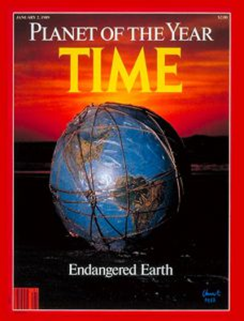
\includegraphics[keepaspectratio]{images/Intro2a_times.png}}

}

\caption{\label{fig-times}``Planet of the Year'' Times Magazine Cover
(1989)}

\end{figure}%

\end{minipage}%

\end{figure}%

Amid the mounting challenges of sustainable development, Christo and
Jeanne-Claude's ``Wrapped Globe'' is a powerful symbol of humanity's
responsibility towards our planet and its resources. The artwork depicts
a globe wrapped in transparent plastic and a filigree net. Meanwhile, in
real life, the world is facing a ``polycrisis'' -- the word used to
describe the many serious crises our Earth is facing, including
ecological crises, growing inequality, excessive national debt, and the
effects of the Covid-19 pandemic, to name but a few. In a polycrisis,
crises are increasingly intertwined and mutually reinforcing (Tooze
2022), and they are mainly caused by a structural dependence on growth
(as measured by gross domestic product, GDP) (Hickel et al., 2022;
Sennholz, 2021); a vicious circle of ever-increasing concentration of
economic and political power in the hands of a few (Piketty, 2014); and
persistent inequalities between and within countries (Chancel et al.,
2021; Milanovic, 2016). And yet, we keep striving for GDP growth in our
society and our economy, in order to maintain and create jobs, finance
our social security systems, secure tax revenues, and fulfil the needs
of companies and industries that depend on growth to exist. As these
expectations become increasingly unrealistic, the idea of decoupling
economic growth from resource consumption has gained traction. However,
there is no empirical evidence that doing so will achieve anywhere near
the scale required to halt multidimensional ecological collapse
(Parrique et al., 2019; Hickel and Kallis, 2020; Wiedmann et al., 2020).

\section*{Full and empty world}\label{full-and-empty-world}
\addcontentsline{toc}{section}{Full and empty world}

\markright{Full and empty world}

The plastic cover and the net wrapped around Christo's globe thus
represent the interconnectedness and interdependence of the Earth's
various elements, and emphasize the need to maintain and preserve these
relationships. A similar idea was described by the economist Herman Daly
(2015), who put forth a concept of the ``empty'' and the ``full'' world.
The empty world describes a situation in which human activities and
resource use have only a minor impact on the environment. In this world,
natural systems are still intact and untouched, and resources are
sufficient to meet human needs. This contrasts with the full world, in
which human activities and resource use overload the ecosystem and
pollute the environment. Since at least the Second World War, we have
pursued an industrialized society and a growth economy. As a result, we
now live in a ``full'' world, where natural resources are scarce and the
balance of ecosystems is under threat. Daly's epiphany came in 1962 upon
reading Rachel Carson's book, Silent Spring, which called for a life in
harmony with nature. Daly was already sceptical about the
hyper-individualism of economic models, and Carson's work highlighted
the conflict between a growing economy and a fragile environment.
Following a lecture by the economist Nicholas Georgescu-Roegen on his
magnum opus, The Entropy Law and the Economic Process (1971), Daly
adopted the idea that the economy was more like an hourglass than a
pendulum, with valuable resources turning into waste and thus largely
irreversibly lost. There is no master plan to counter the polycrisis and
make our economic and social system more sustainable.

\part{Foundations}

\chapter{Understandings and concepts of
sustainability}\label{understandings-and-concepts-of-sustainability}

Where do the concept, mission statement, and guiding principles of
sustainable development come from? How did the concept emerge, how did
it evolve -- and why? The following explanations provide an overview of
the history of sustainability, the political background, and key
conferences and documents. In short, what has made sustainability what
it is today. It's about seeing the big picture. Because only those who
know the past can assess the future.

Sustainability has been the buzzword of recent years, from science to
politics and business to the media. Initially, the term has a positive
connotation because it is associated with the long term, the durable,
and many things are sustainable today: coffee, corporate philosophy,
even tuna pizzas. These are the demands of a consumer society with an
inconsiderate appetite for abundance. First thing in the morning, the
shampoo removes our dandruff ``sustainably''. Then we drive to work at a
company that prides itself on its ``sustainable corporate philosophy'',
and over lunch we discuss sustainable investments. At home, we stick a
tuna pizza in the oven -- sustainably sourced and produced, of course,
as it says on the box.

Today, the term ``sustainability'' is everywhere: it's used in
connection with energy, mobility, building renovation, nutrition,
population development, corporate environmental management, and climate
protection. It's also used in art, culture, design, and advertising.

\begin{figure}[H]

\centering{

\pandocbounded{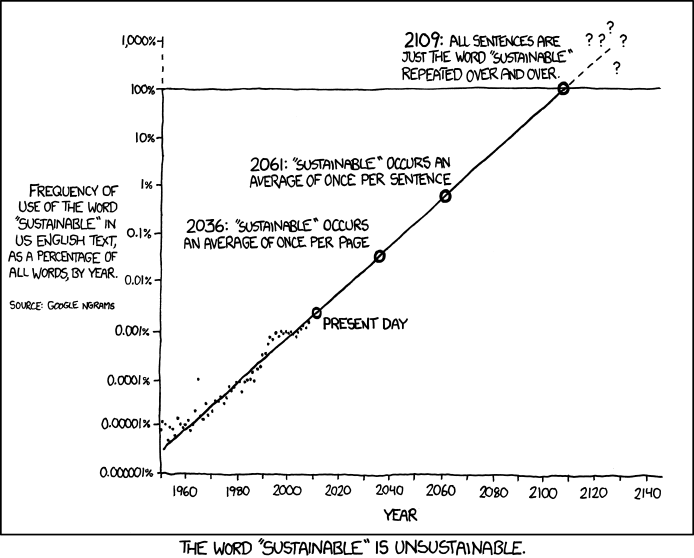
\includegraphics[keepaspectratio]{1_understanding/images/word_sustainable.png}}

}

\caption{\label{fig-word-sustainable}Frequency of use of the word
``sustainable'' in US English texts, as a percentage of all words per
year, based on data from Google Ngrams. Source: https://xkcd.com/1007/}

\end{figure}%

Is the term ``sustainability'' so overused as to slowly become
meaningless? Even if this is the case, we shouldn't abandon key terms
like this lightly. For example, it's still important for companies to
have a sustainability strategy, even if many such strategies are
inadequate or amount to greenwashing. We need to clarify the meaning of
``sustainability'' and hold those who use it to account. And we should
base our interpretation on science and historical developments. The
historical precursors to the sustainability model explained in this
textbook are:

\begin{itemize}
\item
  Start of the discussion about sustainability: Carlowitz's forest
  management principle of 1713
\item
  Clash of economy and ecology First and second UN Development Decades
  (1960s and 1970s)
\item
  The Limits to Growth (1972)
\item
  Brundtland Report (1987)
\item
  Rio Earth Summit 1992 Agenda 21 UN Millennium Development Goals (MDGs)
  (2000--2015)
\item
  2030 Agenda with the Sustainable Development Goals (SDGs) (2015--2030)
\end{itemize}

\section{A normative concept}\label{a-normative-concept}

\begin{figure}[H]

\centering{

\pandocbounded{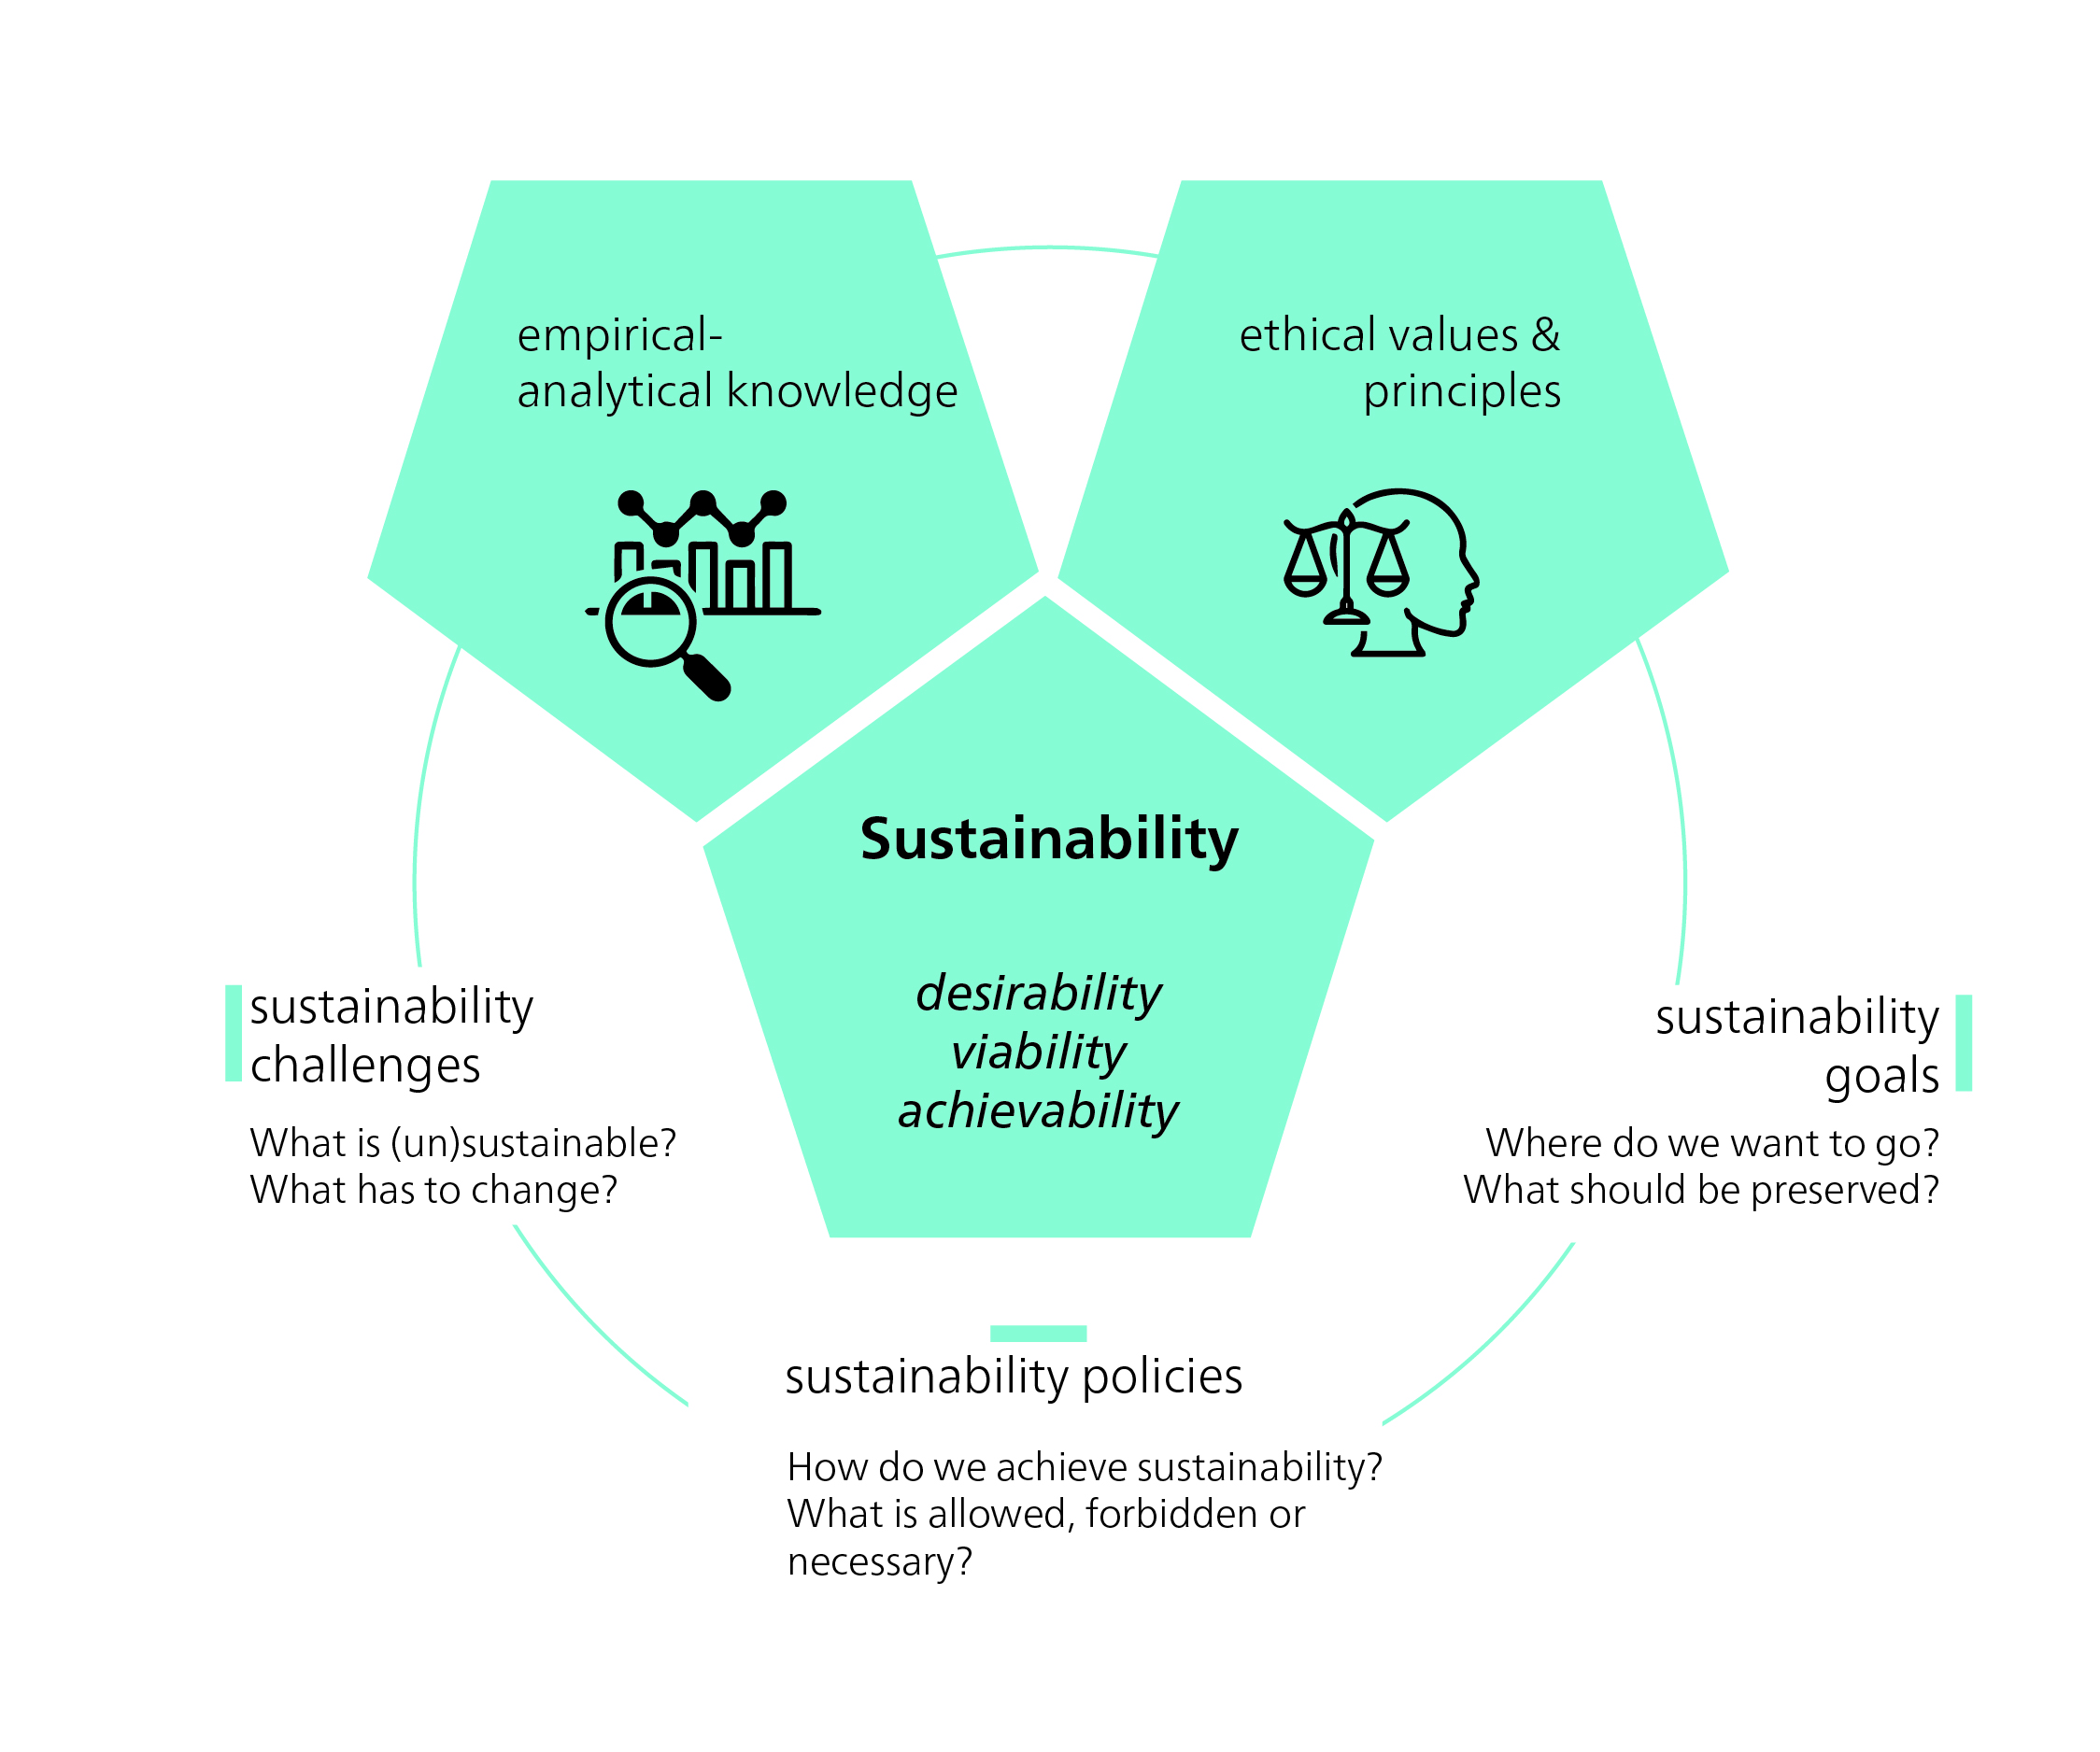
\includegraphics[keepaspectratio]{1_understanding/images/SD_normative.jpg}}

}

\caption{\label{fig-sd-normative}Sustainable Development as a normative
concept (Own illustration).}

\end{figure}%

To achieve sustainability, we need \textbf{sustainable development}: a
strategic process that requires changes in our socio-ecological systems
and institutions. ``Development'' implies controlled improvement, and
the ethical question of what exactly ``better'' means is key. The use of
the term ``development'' has been criticized by some (e.g.~Lang et
al.~2014; Kothari et al.~2019), as it is often equated with unbridled
growth. Unbridled growth of the ``ecological footprint'' -- the
proportion of the biosphere used for human production, consumption, and
waste -- is unsustainable in the long term. Nonetheless, there are
different interpretations of ``development'', ranging from economic
growth to improving quality of life. Sustainable development therefore
remains a stimulating and controversial concept. Sustainability and
sustainable development play a key role in today's political discourse.
The term ``unsustainability'' refers to conditions or developments that
are considered negative, while ``sustainability'' represents a positive
state.

The concept of sustainable development commits us to certain values and
norms that define ethical goals and rules of behaviour. These values and
norms shape our ideas of what we consider a desirable or ``positive''
change. A neutral point of view is not possible, as our perceptions are
shaped by a variety of influences. Our personal experiences, upbringing,
social environment, and cultural background all influence how we see and
interpret the world, including our perceptions of what ``should be'' and
what actions ``should be taken''. Ethics play a key role in determining
how the current situation can be improved to achieve sustainability, by
defining normative goals and limits. Sustainable development is
therefore a conceptual framework that is strongly driven by ethical
considerations.

Sustainability challenges such as poverty reduction and climate change
are therefore ethical challenges. The identification of situations as
sustainability problems (and therefore as ``negative'') and the choice
of solutions are based on ethical values. Sustainability goals are also
based on ethical values, as well as on knowledge of cause-and-effect
relationships. Sustainability issues are often referred to as ``wicked
problems'', because of their complex and pluralistic nature. Global
warming, in particular, has been described as a ``super wicked
problem'', as finding solutions is urgent, political institutions are
often inadequate, and decision-making processes suffer from
short-sightedness.

\section{Global challenges as wicked
problems}\label{global-challenges-as-wicked-problems}

Mike Hulme, author of \emph{Why We Disagree About Climate Change}
(2009), suggests that we view climate change as a ``wicked problem'' of
enormous scale and likely longevity. This approach helps us see climate
change not as a problem that needs to be solved, but as a condition in
which we are directly involved. The categorization of problems as
``wicked'', i.e.~those that do not lend themselves to clear-cut
solutions, originated with the planning theorists Horst Rittl and Melvin
Webber (1973). They argued that planners have to deal with unpredictable
human behaviour, and that some problems are too complicated to be solved
completely. Some ``wicked problems'' may never be fully solved, but we
can learn to cope with them and not let them dominate us.

\begin{figure}[H]

\centering{

\pandocbounded{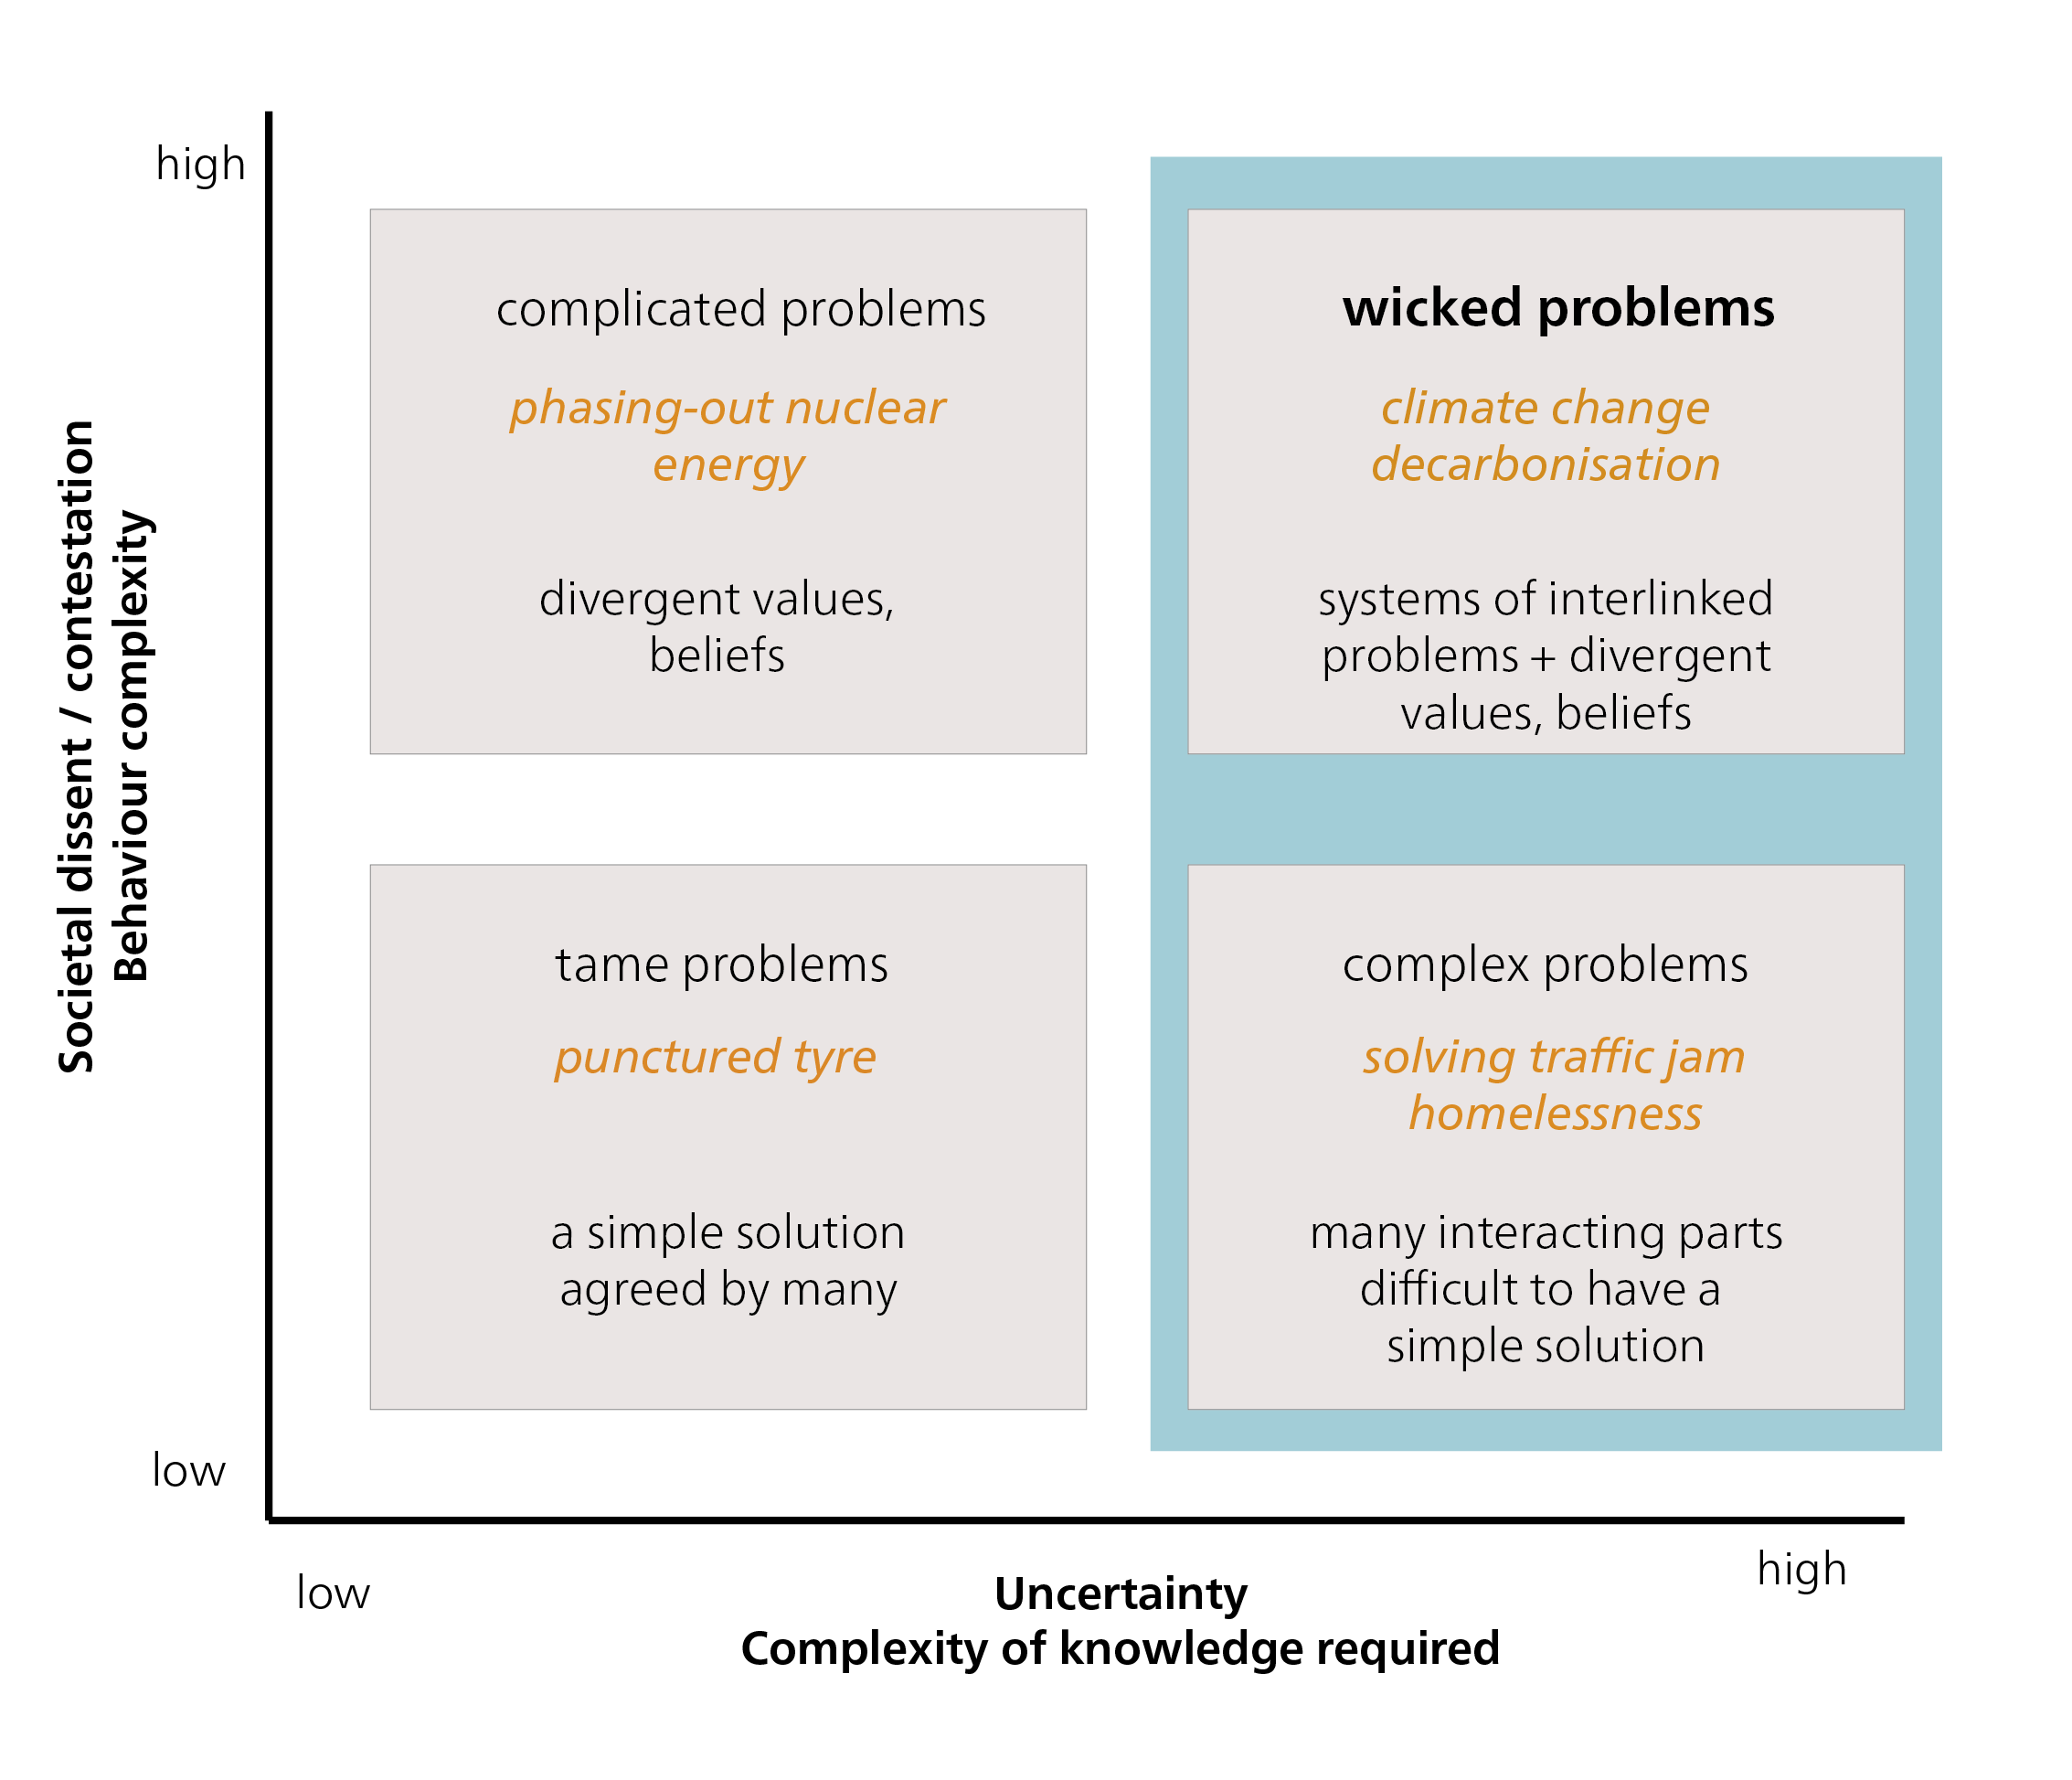
\includegraphics[keepaspectratio]{1_understanding/images/Fig1_3_WickedProblems.png}}

}

\caption{\label{fig-WickedProblems}Sustainability challenges as wicked
problems. Source: Own illustration based on Roth, G. L., \& Senge, P. M.
(1996)}

\end{figure}%

\begin{tcolorbox}[enhanced jigsaw, breakable, left=2mm, arc=.35mm, rightrule=.15mm, opacityback=0, leftrule=.75mm, bottomrule=.15mm, colback=white, toprule=.15mm, colframe=quarto-callout-note-color-frame]

\vspace{-3mm}\textbf{Wicked problems}\vspace{3mm}

According to Bannink and Trommel (2019), wicked problems arise at the
intersection of factual uncertainty and a heterogeneity of preferences
and interests. Wicked problems are characterized by (Rittel \& Weber,
1973; Alford, 2017; Sediri, 2020):

\begin{itemize}
\item
  \textbf{Complexity}: Wicked problems are characterized by many
  interrelated factors and interactions. There are no clear
  cause-and-effect relationships, and changes in one area can have
  unforeseen effects in other areas.
\item
  \textbf{Normative conflicts}: Wicked problems are perceived and
  interpreted differently by different stakeholders and interest groups.
  There is no clear definition or consensus on what exactly the problem
  is, or how it should be solved.
\item
  \textbf{Interdisciplinarity}: Wicked problems require an
  interdisciplinary approach as they involve different topics,
  perspectives, and stakeholders. Finding a solution often requires the
  cooperation and coordination of different disciplines and experts.
  Uncertainty: Incorrect, missing, or inaccessible information about the
  problem situation and about the continuity of the values of the
  variables involved.
\item
  \textbf{No definitive solution}: Wicked problems defy clear-cut
  solutions. They are dynamic, change over time, and require continuous
  adjustment and iterations.
\end{itemize}

Examples of wicked problems include climate change, poverty alleviation,
global health, and sustainability. The complexity and interaction of
different factors in these areas make it difficult to find simple and
clear-cut solutions. Dealing with wicked problems requires a high degree
of reflection, collaboration, and the use of systemic thinking methods.

\end{tcolorbox}

How have we manoeuvred ourselves into the current situation, where
wicked problems pose such a challenge to sustainable development? In
this textbook, we will analyse and learn to understand three key global
challenges:

\begin{itemize}
\item
  the emergence of human-induced global warming;
\item
  the persistence of global poverty and rising inequalities;
\item
  and the threat of species extinction and overexploitation of natural
  resources.
\end{itemize}

The debate about human influence on global warming and climate change
has intensified since the publications of the Intergovernmental Panel on
Climate Change (IPCC). The driving force behind global warming is our
dependence on oil and other fossil fuels for transport, (electricity)
generation, agriculture, and many everyday products. Another wicked
problem is global poverty. Although there have been global efforts to
reduce poverty for decades, the globalized market economy often leads to
increased poverty in certain regions, and the gap between rich and poor
seems to be widening overall (Chancel et al., 2021). High-income
countries have maintained their prosperity and living standards at the
expense of others. These are ``externalized costs'', and they include
environmental degradation. For example, the wealth and living standards
of high-income countries are largely responsible for the threat of
species extinction and the overuse of natural resources (Lessenich,
2018). In addition to the above mentioned ``big three'' -- climate
change, poverty, and biodiversity loss -- there are many other global
sustainability challenges, such as deforestation, desertification,
declining soil fertility, dwindling fish stocks, pollution, wars,
conflicts, and increasing migration.

In analysing these comprehensive challenges we must also consider the
temporal dimension. In 2004, graphs depicting socio-economic and Earth
system trends from 1750 to 2000 were first published, revealing a
dramatic upsurge and aptly termed ``The Great Acceleration'' (Steffen et
al., 2004).

\begin{figure}[H]

\begin{minipage}{0.50\linewidth}
\pandocbounded{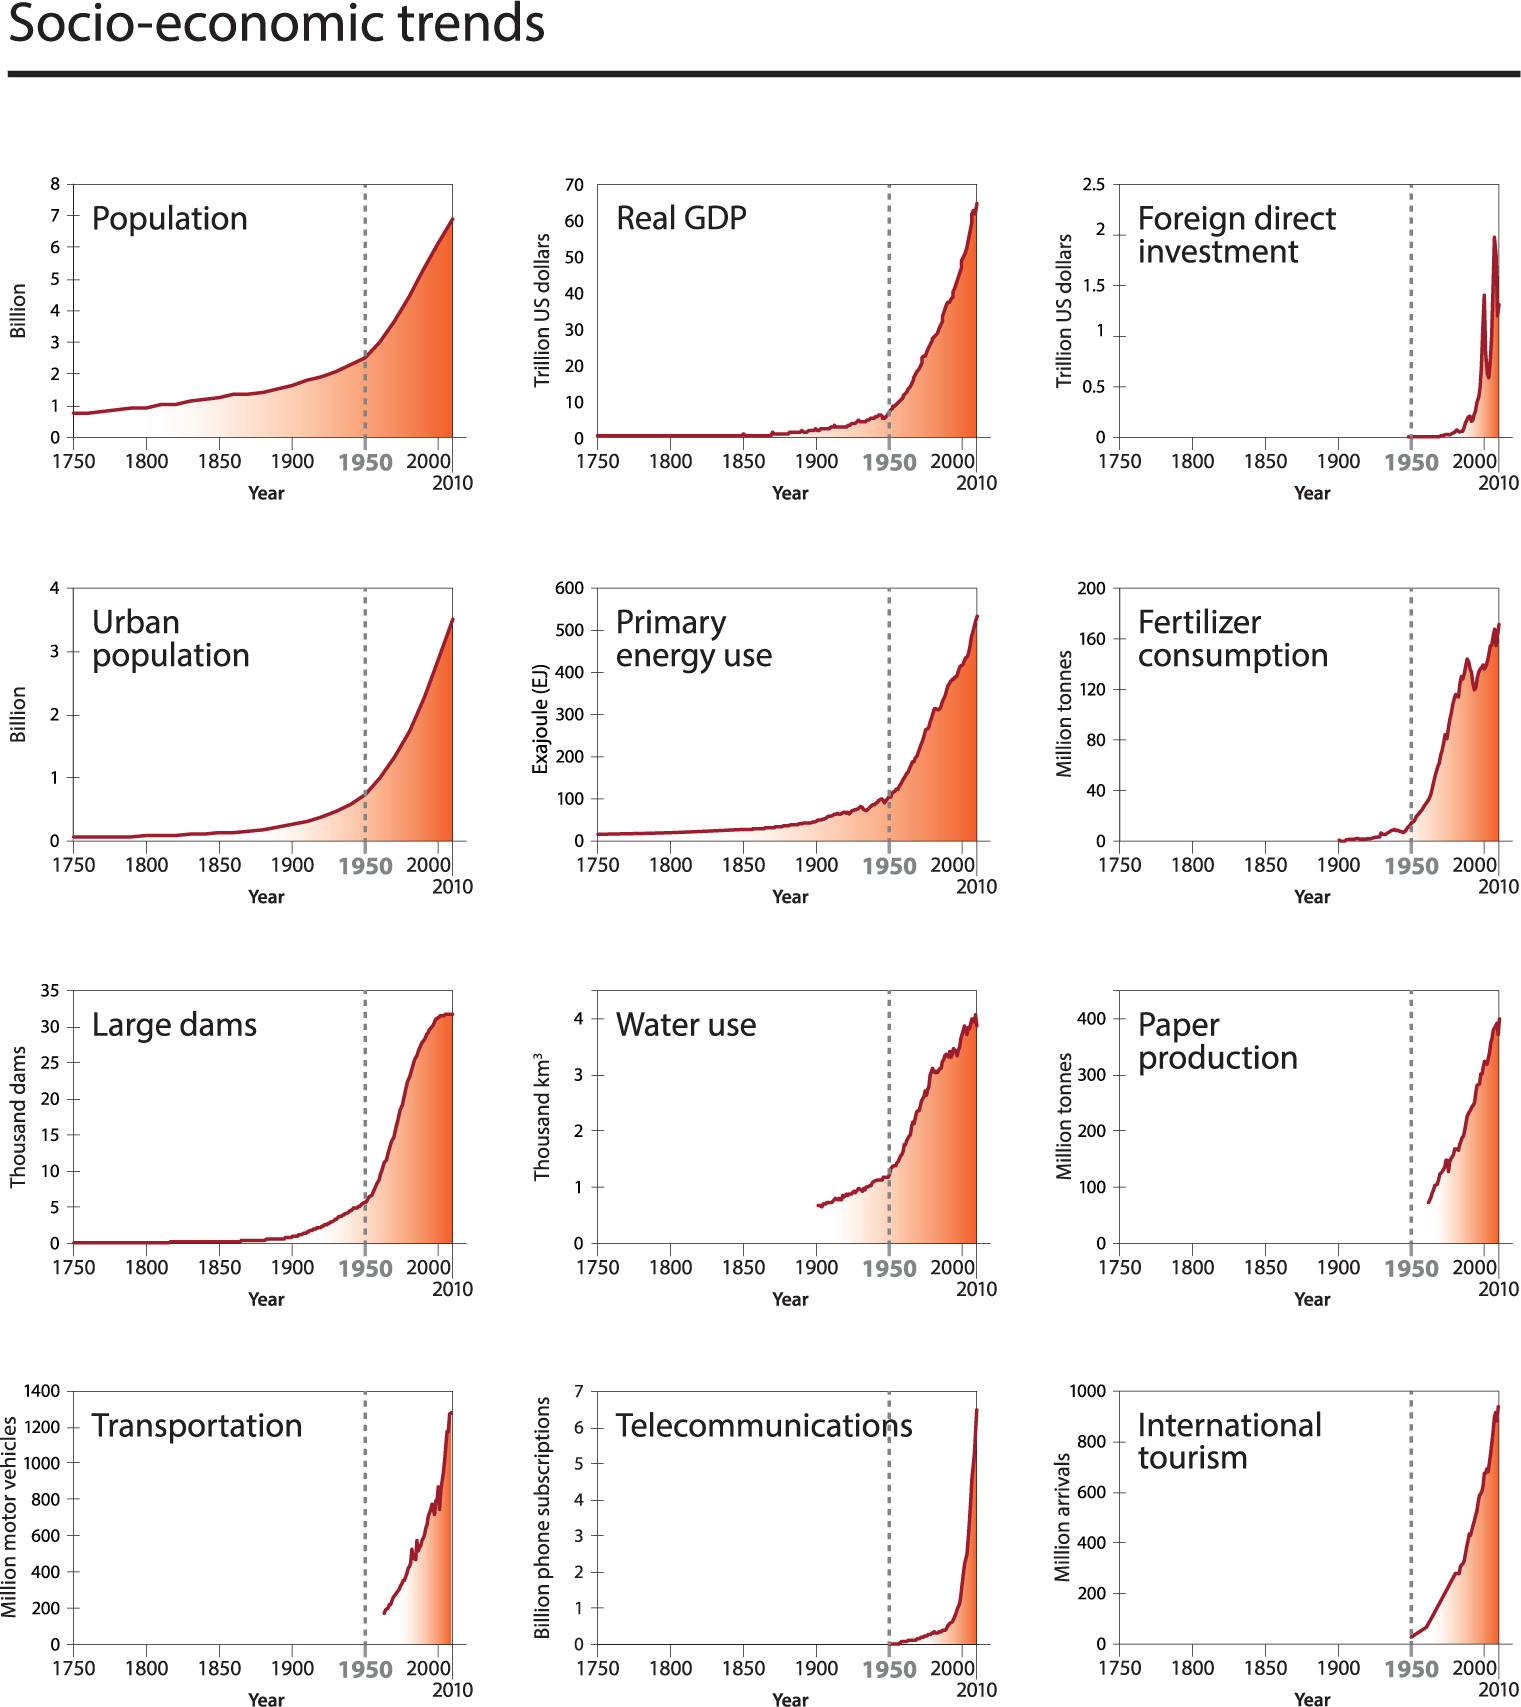
\includegraphics[keepaspectratio]{1_understanding/images/Great-Acceleration_socio-economic_trends.jpg}}\end{minipage}%
%
\begin{minipage}{0.50\linewidth}
\pandocbounded{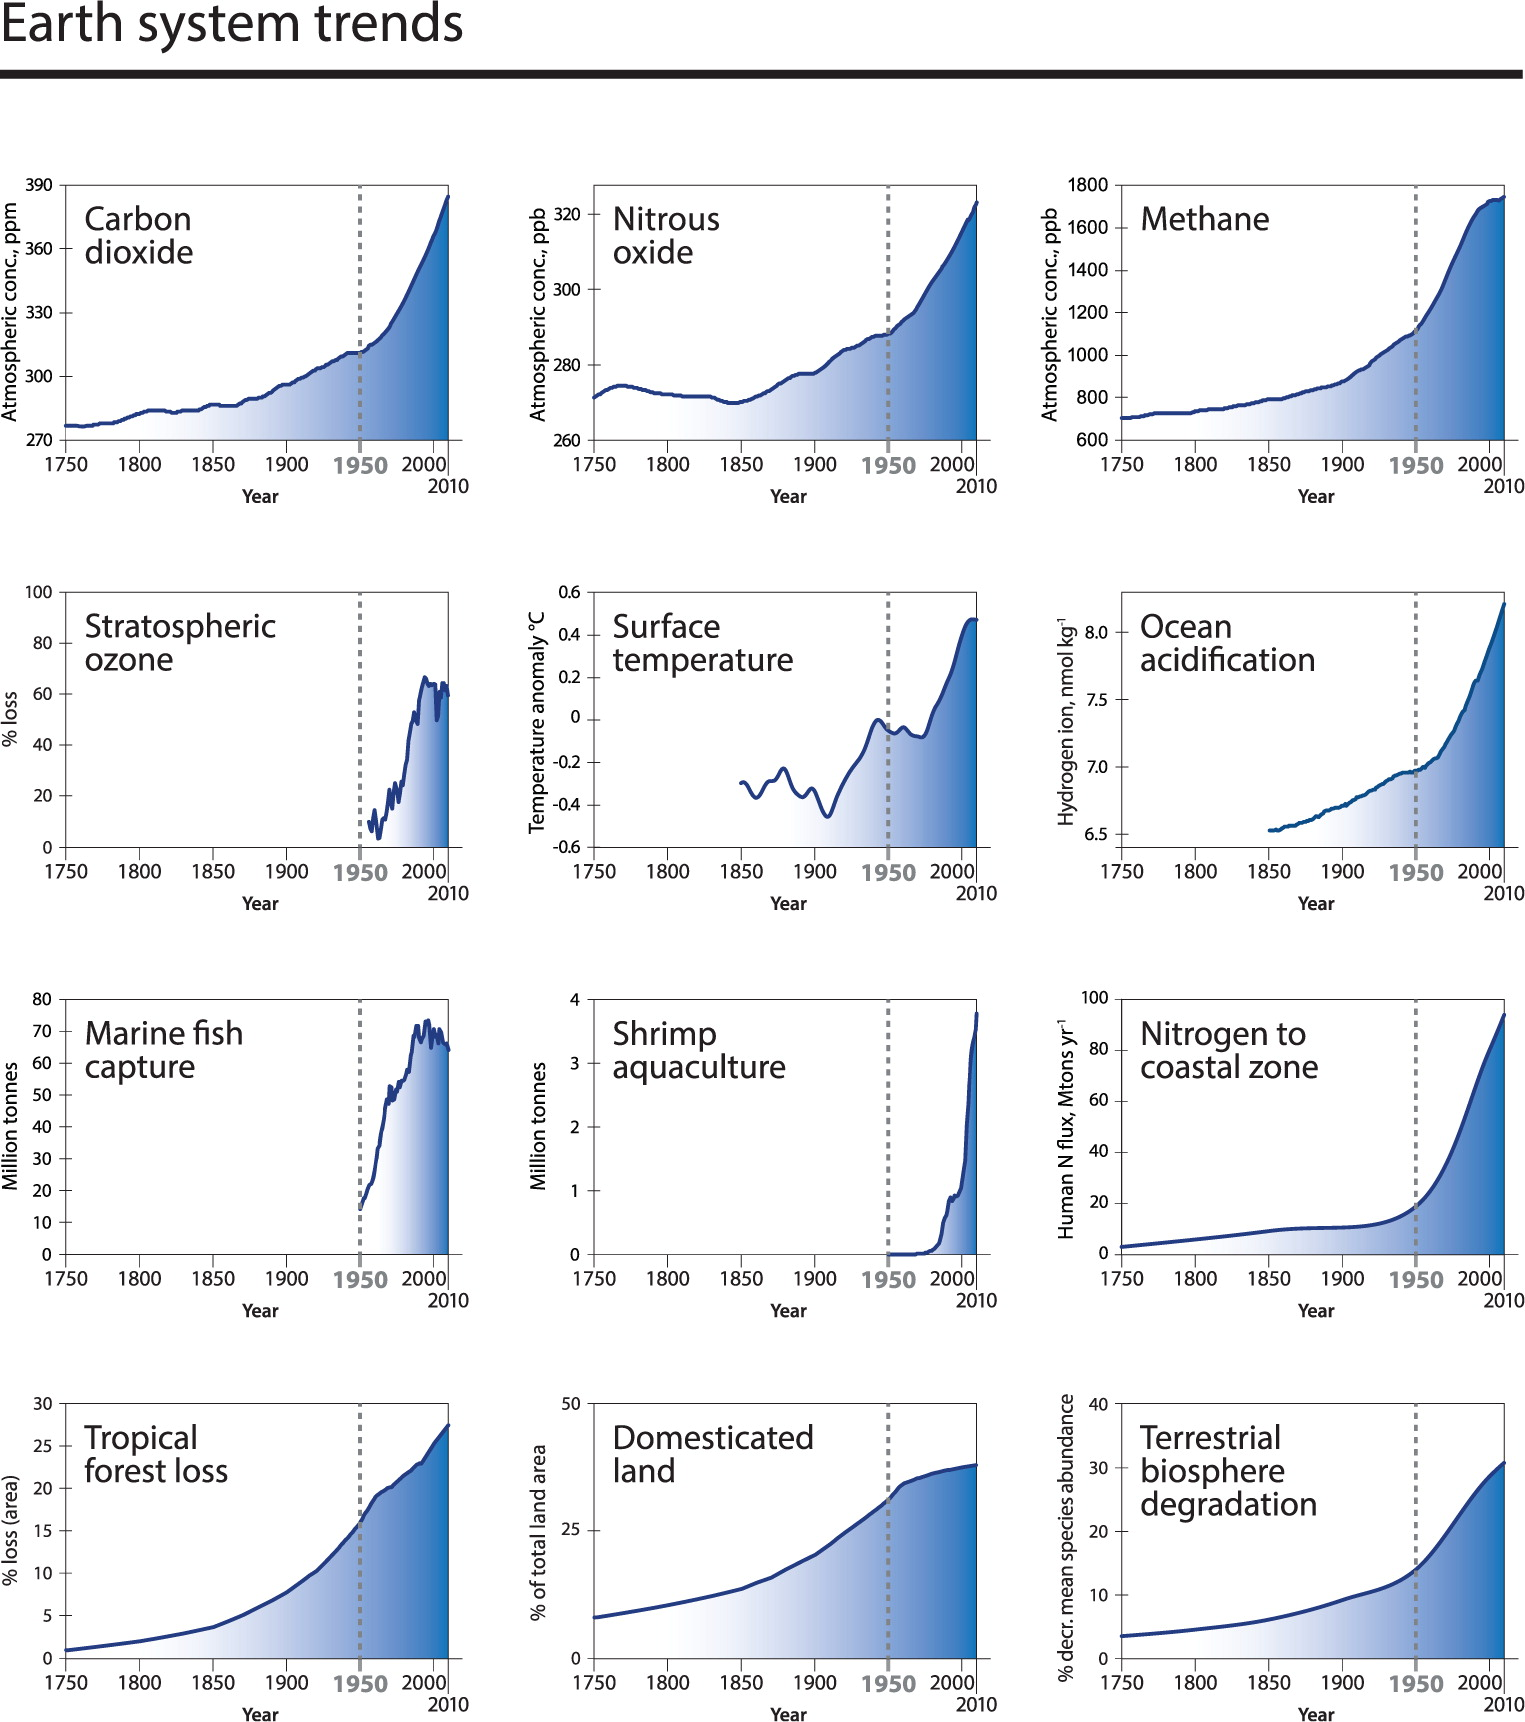
\includegraphics[keepaspectratio]{1_understanding/images/Great-Acceleration_earth-system_trends.jpg}}\end{minipage}%

\caption{\label{fig-acceleration-trends}12 socio-economic and 12 Earth
system trends from 1750 to today are a strong indication that the Earth
system has entered a new state. Source:
\url{https://futureearth.org/2015/01/16/the-great-acceleration/}.}

\end{figure}%

The Great Acceleration described the exponential growth dynamics that
occurred as a result of the Industrial Revolution, which led to a surge
in productivity in the mode of production and a significant increase in
material wealth. At the same time, but to a much lesser extent, there
was a massive increase in natural resource consumption and emissions.
Socio-economic growth went hand in hand with the acceleration of
biophysical trends. Figure~\ref{fig-acceleration-trends} describes some
examples of important biophysical and socio-economic indicators, all of
which start to increase with the Industrial Revolution. From the middle
of the 20th century, the trend towards exponential growth becomes
apparent.

\begin{tcolorbox}[enhanced jigsaw, left=2mm, arc=.35mm, titlerule=0mm, opacityback=0, leftrule=.75mm, title={The Wheat and Chessboard Problem: an illustration of exponential growth}, breakable, bottomtitle=1mm, rightrule=.15mm, coltitle=black, toptitle=1mm, bottomrule=.15mm, colback=white, opacitybacktitle=0.6, colbacktitle=quarto-callout-tip-color!10!white, toprule=.15mm, colframe=quarto-callout-tip-color-frame]

The Wheat and Chessboard Problem is a mathematical problem often used to
illustrate the concept of exponential growth. In the story, a servant
asks the king to fill every square on a chessboard with grains of wheat,
doubling the number on each square. Growth starts slowly, but with each
doubling, the number of grains increases exponentially. By the 50th
square, the number of rice grains would be large enough to cover
Berlin's 365-metre-high television tower on Alexanderplatz. This story
illustrates the immense power of exponential growth and its impressive
results. Understanding the concept of exponential growth is crucial to
analysing phenomena such as population growth, technological progress,
environmental change, and the spread of disease. It illustrates how even
small changes or developments in a system can have a significant impact.
History reminds us that we need to think carefully about how we manage
such growth and the long-term consequences it can have.

\end{tcolorbox}

Resource extraction has increased significantly in recent decades, from
22 billion tonnes in 1970 to 70 billion tonnes in 2010 (UNEP, 2016).
Global warming is another pressing issue. The latest IPCC report (IPCC,
2023) predicts an increase in global average temperature of between 1.5
and 5.8 degrees Celsius, depending on the scenario and future emissions.
Another alarming phenomenon is deforestation. Every two seconds, an area
of forest the size of a football field is cut down -- an area the size
of New York City every day. And then there is the decline in
biodiversity, marked by the extinction of animal and plant species,
which threatens the ecological diversity of our planet.

The Great Acceleration (Figure~\ref{fig-acceleration-trends}) describes
the observable and measurable (negative) developments of key
socio-economic and biophysical indicators since 1950. The causes of
these negative developments can be far removed from the place where the
problems arise or become most evident. For example, job losses in one
country may be caused by a multinational company's decision to relocate
part of its operations to another country, in order to maximize profits.
We cannot hope to fix such issues unless we understand how the system --
in this case, the globalized economy -- works. Similarly, we need to
understand the Earth's global climate systems to imagine what the
consequences of global warming might be in a particular area or region.

This is why many of the methods and concepts of sustainability science
require systemic thinking. A systemic thinking approach often begins
with brainstorming to create a ``rich picture'' of all the factors you
need to consider in order to understand the current behaviour of the
system in question. For example, in the case of a multinational company
closing a particular business unit, these would be the factors that
might influence the decision to continue, expand, or close certain
business units. While an initial mapping might look overly complex or
even messy, creating a linear flowchart can help clarify the flows of
inputs and influences. This kind of mapping may already reveal
opportunities to reassess the relevant influences and redesign the
system to avoid unwanted outcomes. However, further work may be required
to develop ``conceptual models'' of the system that identify unforeseen
opportunities for improvement.

Incorporating systemic thinking into the methods and concepts of
sustainability science enables us to tackle the complexity of problems
and develop sound strategies for sustainable development. Systemic
thinking thus provides an important basis for understanding and shaping
the different understandings and concepts of sustainable development, as
the next chapter discusses in more detail.

\section{Sustainability: When did we start talking about
it?}\label{sustainability-when-did-we-start-talking-about-it}

In 1713, Saxony's chief mining officer, Hans Carl von Carlowitz,
demonstrated the necessity and possibility of ``sustainable forestry''
in a book entitled \emph{Sylvicultura oeconomica, oder hauswirthliche
Nachricht und Naturmässige Anweisung zur wilden Baum-Zucht (Sylvicultura
oeconomica, A Guide to the Cultivation of Native Wild Trees)}. Another
sustainability pioneer was Duchess Anna Amalia, the mother of Duke Carl
August. In the late 1700s, she initiated the world's first forestry
reform, which was aimed at ensuring a continuous and steady supply of
timber. At that time, Europe had an insatiable appetite for materia
prima, or raw materials needed for building ships and houses, and for
cooking and heating. This demand threatened to deplete resources and
endanger their long-term survival.

In the 18th century, scholars in Germany as well as in other parts of
Europe addressed the finite nature of natural resources. Unlike von
Carlowitz, however, no one spoke about sustainability. One important
aspect was the provision of food for a growing population. Before
industrialization, economic growth was largely determined by nature as a
factor of production, such as the number of mines or ships built, or the
amount of land available for farming. However, Thomas Robert Malthus, a
British economist, warned that food production would not be able to keep
up with the rapid population growth following the Industrial Revolution.
Malthus believed that the population would grow at a exponential rate,
while food production would increase at a linear rate. Although
Malthus's thesis did not come true in the dramatic way he predicted, his
work is often regarded as the first systematic treatise on the limits to
growth in a finite world.

For a time, Malthus's ideas fell out of favour, as unlimited growth
seemed possible due to the Industrial Revolution and the rise of
capitalism. Talk of natural limits didn't resurface until the mid-20th
century, when a ``neo-Malthusian'' perspective re-emerged in the context
of the Club of Rome (founded in 1968), debates on planetary boundaries,
and critiques of growth. While Malthusianism traditionally focuses on
external, physical limits to growth, the ecological economist, Giorgos
Kallis, proposes a different approach. Kallis (2019) advocates personal
moderation and voluntary restraint, an approach to life that has deep
roots in Romanticism and ancient Greek philosophy. He argues for an
inner limit to our wants, to free us from the economic assumption of
scarcity and the associated obsession with growth. While acknowledging
the reality of external limits, Kallis believes they should not dominate
the environmental argument against limitless growth. Kallis therefore
asks whether it makes sense to frame climate change primarily as a
problem of external limits, of scarcity, or of a finite atmosphere that
cannot absorb any more of our emissions.

In the Malthusian logic, we would have to ever increase our production
to meet the needs of a world with limits. As long as this mindset
persists, the focus is on how we can exceed those limits, and how we can
push the capacity of the climate to absorb a growing population and its
demands.

\subsection{The clash of economy and
ecology}\label{the-clash-of-economy-and-ecology}

Originally, sustainability was a principle of resource economics that
combined the economic goal of maximizing long-term forest use with
ecological conditions for regrowth. In the 19th century, the concept of
an `eternal forest' emerged with the aim of putting an end to
overexploitation and ensuring a long-term supply of wood, a vital raw
material. Forestry scientists such as Heinrich Cotta developed
mathematical methods for calculating timber stocks and growth. Over
time, however, the focus shifted towards the pure yield theory, which
focused on short rotation periods, high-yield monocultures and
maximizing financial benefits. The focus was suddenly on the highest
possible direct cash yield instead of a steady high timber yield.
Natural cycles were replaced by capitalist dynamics; exchange value took
precedence over utility value. This devalued the guiding principle of
sustainability, and it took over a hundred years, until the 1960s and
70s, for the scientific disciplines of ecology and sustainability to
regain prominence.

\subsection{Club of Rome and The Limits to
Growth}\label{club-of-rome-and-the-limits-to-growth}

\begin{quote}
``If the present growth trends in world population, industrialization,
pollution, food production, and resource depletion continue unchanged,
the limits to growth on this planet will be reached sometime within the
next one hundred years.'' Meadows et al.~(1972), p.~23
\end{quote}

\begin{figure}[H]

\centering{

\pandocbounded{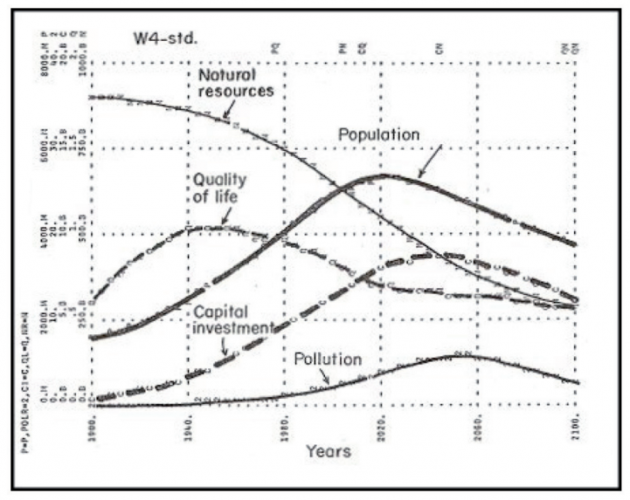
\includegraphics[keepaspectratio]{1_understanding/images/Basic-model.png}}

}

\caption{\label{fig-basic-model}The ``Basic model'' of the simulation
carried out at MIT, published in the autumn of 1970. Source:
\url{https://donellameadows.org/}.}

\end{figure}%

In 1972, the Club of Rome published a report, \emph{The Limits to
Growth}, which introduced a much broader understanding of
``sustainability''. Scientists begin to call for a global state of
equilibrium, or homeostasis, that would only be possible through
coordinated international action. They integrate economic, ecological,
and social aspects of sustainability and use the model of the dynamics
of complex systems (``system dynamics'') to understand the world. They
take into account the interactions between population density, food
resources, energy, materials, capital, environmental degradation, and
land use. Computer simulations of different scenarios show similar
results: a catastrophic decline in the world's population and living
standards within 50 to 100 years, if current trends continue. The
problem with the resource- and emission-intensive industrialized
societies is that growth is not linear but exponential. In the long run,
this kind of growth leads to collapse. And ecological collapse can only
be prevented through a course correction, argued the report.

The \emph{Meadows Report}, as it is also known, was heavily criticized
for its predictions and methods. Some critics argued that the system
dynamics model was too simplistic and failed to consider important
factors such as technology and innovation. Others said insufficient
account was taken of human adaptability and the possibility of political
solutions and change. Others yet criticized what they called a
Malthusian outlook and a pessimistic view of the future. Despite these
criticisms, however, the report sparked an important debate about
sustainability and the need to protect the environment.

A year later, E.F. Schumacher published \emph{Small is Beautiful:
Economics as if People Mattered} (1973). Schumacher challenged the
prevailing notion of limitless economic growth and technological
progress. Instead, he advocated for a sustainable, human-centred economy
that respects local communities and the environment. Schumacher argued
that a decentralized economy, based on human values, not just profit,
would create a better future for all. He also emphasized the importance
of education and cultural development in creating a sustainable society.

\section{From the development debate to the sustainability
debate}\label{from-the-development-debate-to-the-sustainability-debate}

Worsening air and water pollution helped raise the profile of
environmental issues in politics and the media. Greenpeace was founded
in 1971. In the 1960s and 1970s, Paul Crutzen and his research team
studied the impact of nitrogen oxides on the ozone layer, predicting
that this layer would be greatly depleted by human-made CFCs. The use of
CFCs in refrigerators and air conditioners was subsequently banned. In
response to the growing importance of environmental issues, the United
Nations organized the first ever major environmental conference in
Stockholm in 1972. The United Nations Conference on the Human
Environment, as it was called, led to the creation of the United Nations
Environment Programme (UNEP) and independent environment ministries in
many countries.

\begin{figure}[H]

\centering{

\pandocbounded{\includegraphics[keepaspectratio]{1_understanding/images/Demonstration_air-pollution_Zürich.png}}

}

\caption{\label{fig-demo-air-poll}Demonstration against air pollution,
Zurich, December 1986. Source: Schweizerisches Sozialarchiv/Gertrud
Vogler.}

\end{figure}%

The emergence of environmental problems in the 1970s and 1980s coincided
with the first ``development crises'' after the Second World War. In
those days we still spoke of ``underdeveloped countries''. Following the
success of the Marshall Plan in rebuilding Europe after World War II, it
was assumed that similar programmes, such as a Marshall Plan for Africa,
would lead to a rapid catch-up in socio-economic development of the poor
countries of the Global South. But the 70s and 80s proved otherwise.
Even exemplary countries such as Mexico and Brazil succumbed to debt
crises, demonstrating that achieving socio-economic development and
overcoming poverty were far more complex challenges.

From then on, it was clear that issues related to development and the
environment had to be considered together at the intergovernmental
level. In 1983, the United Nations set up a World Commission on
Environment and Development, chaired by the Norwegian Prime Minister,
Gro Harlem Brundtland.

\subsection{Brundtland Commission}\label{brundtland-commission}

Gro Harlem Brundtland appointed 22 commission members, ¾ of whom were
from the Global South. During this time, the Soviet Union, facing
economic stagnation, was beginning to change political course. As the
arms race with the US had contributed to a substantial budget deficit,
Mikhail Gorbachev, the newly appointed General Secretary of the
Communist Party of the Soviet Union, introduced major reforms. At the
same time, a new world view and global consciousness were starting to
emerge. It was against this background that the Brundtland Commission
was tasked with drawing up a report on the perspective of global,
sustainable, environmentally friendly development up to and beyond the
year 2000. The report presented in 1987 was entitled \emph{Our Common
Future}, but it's often referred to as the \emph{Brundtland Report}.

The Brundtland Report found that global environmental problems were
mainly due to unsustainable consumption and production patterns in the
North and severe poverty in the South. The overexploitation of nature
and depletion of natural resources were exacerbating inequalities (of
income and wealth), increasing absolute poverty, and posing a threat to
peace and security. The Report sought to develop a fair and just
definition of sustainability:

\begin{quote}
``Sustainable development is development that meets the needs of the
present without compromising the ability of future generations to meet
their own needs.'' (WCED 1987)
\end{quote}

This definition introduced an ethical perspective into the
sustainability debate, placing the principle of responsibility at the
centre for both present and future generations. By focusing on human
needs, the Brundtland Commission adopted an anthropocentric position.
The Brundtland Commission identified three key principles for analysing
problems and guiding action: a global perspective, the
interconnectedness of environment and development, and the pursuit of
justice, or equity. The concept of justice/equity was further divided
into two distinct perspectives:

\begin{enumerate}
\def\labelenumi{\arabic{enumi}.}
\tightlist
\item
  The intergenerational perspective: Responsibility for future
  generations.
\item
  The intragenerational perspective: Responsibility for people living
  today, particularly in developing countries, and ensuring equity
  within countries.
\end{enumerate}

\begin{tcolorbox}[enhanced jigsaw, left=2mm, arc=.35mm, titlerule=0mm, opacityback=0, leftrule=.75mm, title={Sustainability and sustainable development}, breakable, bottomtitle=1mm, rightrule=.15mm, coltitle=black, toptitle=1mm, bottomrule=.15mm, colback=white, opacitybacktitle=0.6, colbacktitle=quarto-callout-note-color!10!white, toprule=.15mm, colframe=quarto-callout-note-color-frame]

The concepts of ``sustainability'' and ``sustainable development''
differ in focus. Sustainability is static; it emphasizes a consistent
state, while sustainable development is the dynamic process of achieving
that state, implying movement and referring to something that is
emerging.

\end{tcolorbox}

\section{From Rio 1992 to today}\label{from-rio-1992-to-today}

After the Brundtland Report's call for international action, the focus
turned to translating demands and proposals into binding treaties and
conventions. The UN chose a conference as an instrument for this, and it
was held exactly 20 years after 1972 Stockholm Conference, the first
global environmental conference. The UN Conference on Environment and
Development held in Rio de Janeiro, Brazil, in June 1992 -- also known
as the Earth Summit -- was the largest international conference to date,
with delegates from over 170 nations.

The Rio Earth Summit adopted the following five documents:

\begin{itemize}
\tightlist
\item
  A Forest Declaration, aimed at the ecological management and
  protection of the world's forests;
\item
  A Climate Protection Convention committing states to reducing
  greenhouse gas emissions worldwide to 1990 levels;
\item
  A Biodiversity Convention to combat the decline in biodiversity
  through steps that are binding under international law;
\item
  The Rio Declaration on Environment and Development; and • Agenda 21,
  the best known of the five agreements, according to which national
  governments are responsible for implementing the sustainability model
  in their countries.
\end{itemize}

The Rio Declaration on Environment and Development emphasizes that
long-term economic progress is only possible using an ecosystem
approach. This, in turn, requires a new and equitable global partnership
among governments, people, and key societal groups. To achieve this,
international agreements are necessary to protect the environment and
the development system. The Rio Declaration established key principles
of sustainable development, including precaution and polluter pays. For
example, Principle 15 states: ``In order to protect the environment, the
precautionary approach shall be widely applied by States according to
their capabilities. Where there are threats of serious or irreversible
damage, lack of full scientific certainty shall not be used as a reason
for postponing cost-effective measures to prevent environmental
degradation''. (UN 1992)

In December 1992, the Commission on Sustainable Development (CSD) was
established to ensure effective follow-up of the Summit.

\subsection{Agenda 21: Think globally -- act
locally}\label{agenda-21-think-globally-act-locally}

Agenda 21, which contains 40 chapters, addresses all critical policy
areas and actions for sustainable development. According to the
Preamble, ``\ldots integration of environment and development concerns
and greater attention to them will lead to the fulfilment of basic
needs, improved living standards for all, better protected and managed
ecosystems and a safer, more prosperous future. No nation can achieve
this on its own; but together we can -- in a global partnership for
sustainable development.'' (UN CSD, 1992)

\subsection{The Millenium Development Goals
(MDGs)}\label{the-millenium-development-goals-mdgs}

The core principles of Agenda 21 -- empowering women, protecting the
environment, and promoting an equitable and inclusive society -- laid
the foundation for the Millennium Development Goals (MDGs) . Adopted by
the UN in 2000, the MDGs comprised eight specific goals to be achieved
by 2015. Although not all of these goals were met, the MDGs raised
significant awareness of the need for sustainable development. The MDGs
were succeeded by the Sustainable Development Goals (SDGs), which were
adopted by the UN in 2015.

\subsection{Rio+20}\label{rio20}

The UN Conference on Sustainable Development, or Rio+20, was held in Rio
de Janeiro in 2012, 20 years after the historic 1992 Earth Summit that
adopted Agenda 21. The main objective of Rio+20 was to reaffirm global
political commitment to sustainable development. Participants, including
government leaders and NGO and private sector representatives, discussed
a wide range of issues, including poverty eradication , environmental
protection, sustainable energy, food security, and resource management.
The Summit's key outcome was the adoption of a declaration entitled
``The Future We Want''. This declaration renewed the international
community's commitment to sustainable development and to the Rio
Principles and past action plans , and outlined further measures to
achieve these goals. In addition, Rio +20 paved the way for a universal
development framework to define global sustainability goals and
priorities beyond 2015.

\subsection{The 2030 Agenda and the Sustainable Development Goals
(SDGs)}\label{the-2030-agenda-and-the-sustainable-development-goals-sdgs}

\begin{quote}
``We are the first generation that can put an end to poverty and we are
the last generation that can put an end to climate change, so we
{[}must{]} address climate change.'' Ban-Ki Moon, UN Secretary General
2007--2016, on the 2030 Agenda
\end{quote}

Rio +20 laid the foundation for the 2030 Agenda, which the UN adopted in
2015. The 2030 Agenda builds on the results of Rio+20 and sets out a
comprehensive framework for sustainable development. The 2030 Agenda is
based on five key principles or pillars (the 5 Ps) and introduces the 17
Sustainable Development Goals (SDGs), which aim to create a sustainable
and just world by 2030.

\begin{tcolorbox}[enhanced jigsaw, left=2mm, arc=.35mm, titlerule=0mm, opacityback=0, leftrule=.75mm, title={The 5 Ps of the SDGs}, breakable, bottomtitle=1mm, rightrule=.15mm, coltitle=black, toptitle=1mm, bottomrule=.15mm, colback=white, opacitybacktitle=0.6, colbacktitle=quarto-callout-note-color!10!white, toprule=.15mm, colframe=quarto-callout-note-color-frame]

The 5 Ps represent five key principles of sustainability : People,
Planet, Prosperity, Peace, and Partnership.

\textbf{People}: This P stands for the aim to promote social justice,
equal opportunities, good health, and education for all people. It also
seeks to end poverty, promote gender equality, and improve people's
well-being.

\textbf{Planet}: The aim of this P is to protect natural resources and
to use them sustainably, to preserve biodiversity, to protect the
climate, and to reduce pollution. Overall, it seeks to preserve our
planet and promote sustainable environmental practices.

\textbf{Prosperity}: This refers to economic growth, sustainable
production and consumption patterns, and the creation of jobs and
economic prosperity for all. This P aims to promote a strong and
sustainable economy that benefits all people.

\textbf{Peace}: This is about promoting peace, justice, good governance,
and strong institutions. It's also about preventing conflict, reducing
violence, and building inclusive societies.

\textbf{Partnership}: This refers to the importance of global
cooperation, partnerships, and solidarity among all stakeholders. It's
about working together to implement the 2030 Agenda, and sharing
resources, experience, and knowledge.

\end{tcolorbox}

\subsection{2015 Paris Climate Agreement}\label{paris-climate-agreement}

The Paris Climate Agreement of 2015 is a landmark international
agreement adopted at the 21st Conference of the Parties (COP 21) to the
UN Framework Convention on Climate Change (UNFCCC) in Paris. The
Agreement aims to limit the global temperature rise to well below 2
degrees Celsius compared to pre-industrial levels, and to endeavour to
limit it to 1.5 degrees Celsius. The Paris Agreement is based on the
principle of common but differentiated responsibilities and respect for
national circumstances. It encourages all countries to take action to
reduce their greenhouse gas emissions and to set themselves voluntary
climate targets, known as Nationally Determined Contributions (NDCs).

The 2015 Paris Climate Agreement applies to every country that has
ratified it, including Switzerland . As a Party to the Agreement,
Switzerland has committed to contributing to the global reduction of
greenhouse gas emissions and to implementing the Agreement's objectives.

\subsection{Conclusion -- there is progress, but it's too
slow}\label{conclusion-there-is-progress-but-its-too-slow}

While there has been some progress in institutionalizing and
disseminating sustainability approaches in business, policymaking, and
other areas, a large number of studies show that the world as a whole is
on an unsustainable course (see the
\href{https://www.sdgital2030.ch/countryreport}{Voluntary National
Review of Switzerland 2022}). A similar picture is painted by various
studies on the global environmental situation, such as UNEP's Global
Environment Outlook 5 (GEO-5) published in 2012, the 2010 Millennium
Development Goals Report (MDGs Report 2010), and reports on the 2030
Agenda and climate change (IPCC 2022). As these studies show, the
international community is a long way from sustainable,
intergenerationally equitable ecological, social, and economic
development.

For example, international climate policies have not stopped the rise in
CO2 emissions, the main cause of human-induced climate change, which
have risen by around 50\% since 1990. Species loss continues to
accelerate in many places. The global fight against poverty falls short
of the desired goals, and economic globalization over the past three
decades has worsened socio-economic inequality in many countries, often
linked to sociopolitical and sociocultural disparities.

\section{The guiding principle of sustainable development as a normative
concept}\label{the-guiding-principle-of-sustainable-development-as-a-normative-concept}

Turning the concept of sustainability into action and developing
implementation strategies is a major challenge for our society. There
are different understandings and concepts of sustainability and
sustainable development, with no consensus on how to achieve
sustainability and which measures to prioritize. Some of these
understandings are presented below. The diversity of approaches reflects
the different perspectives and interests of different stakeholders. To
navigate this complexity, we need to reconcile economic, social, and
environmental considerations. This requires an integrative approach. The
challenge is to define common goals and develop strategies to achieve
sustainability at all levels -- global, national, regional, and local.
We need broad societal participation and dialogue and cooperation
between governments, business, civil society, and research institutions,
to find solutions and drive the necessary change.

\begin{quote}
``When powerful metaphors become fashionable buzzwords, we risk that
diversity is accompanied by vagueness, i.e.~the phenomenon of a term
that has several meanings that `have so much in common that it is
difficult to separate them'\,'' (Strunz 2012: 113 as cited in Feola
2015: 377).
\end{quote}

The concept of sustainability usually has a positive connotation, but it
can be viewed from different perspectives. In order to function as a
guiding principle (in an ecological, social, and economic sense), it
requires clear criteria. But what grounds can we use to define these
criteria?

According to Hirsch Hadorn \& Brun (2007), ``sustainable development''
should:

\begin{itemize}
\tightlist
\item
  Fulfil \emph{needs}\ldots{}
\item
  \ldots in a \emph{just} way,
\item
  \ldots with a view to people living today and in the future, and
\item
  taking into account the diversity of values and the limits to which
  nature can be used.
\end{itemize}

The guiding principle of sustainable development is therefore not only
the result of scientific research, but is first and foremost a
normative, ethically based concept. It brings together ``ethical and
analytical ideas'' and formulates ``norms that express what is desirable
and what should happen'' (Renn et al.~2007: 39). As a result,
sustainable development is a social process of negotiation and
decision-making -- of searching, learning, and gaining experience --
that is guided by ethical considerations. Accordingly, sustainability
research must always be aware of its involvement in social processes of
perception and evaluation.

\subsection{What values and norms should we be guided by, and
why?}\label{what-values-and-norms-should-we-be-guided-by-and-why}

Moving from the concept of sustainable development to its
implementation, ethics come into play. Ethics provide evaluation
criteria, methodological procedures, or principles for ``justifying and
criticizing rules of action or normative statements about how we should
act'' (Fenner 2008, p.~5). Ethics also help to structure and justify
complex decisions that arise in dilemma situations. In contrast to
problems with single solutions, a dilemma is more complex and involves
trade-offs and the weighing up of different options for action. Ethics
provide orientation and decision-making structures that provide a
framework for finding a suitable course of action in such situations.
The core function of ethics is therefore not to solve monocausal
problems, but to structure and categorize complex dilemmas.

Put simply, ``morality'' refers to personal or social beliefs about
right and wrong, while ``ethics'' is the philosophical study of these
beliefs. Ethics studies the rules and principles that ``ought'' to
govern human behaviour. Ethics can be divided into general and applied
ethics (Figure~\ref{fig-branches-ethics}).

\begin{figure}[H]

\centering{

\pandocbounded{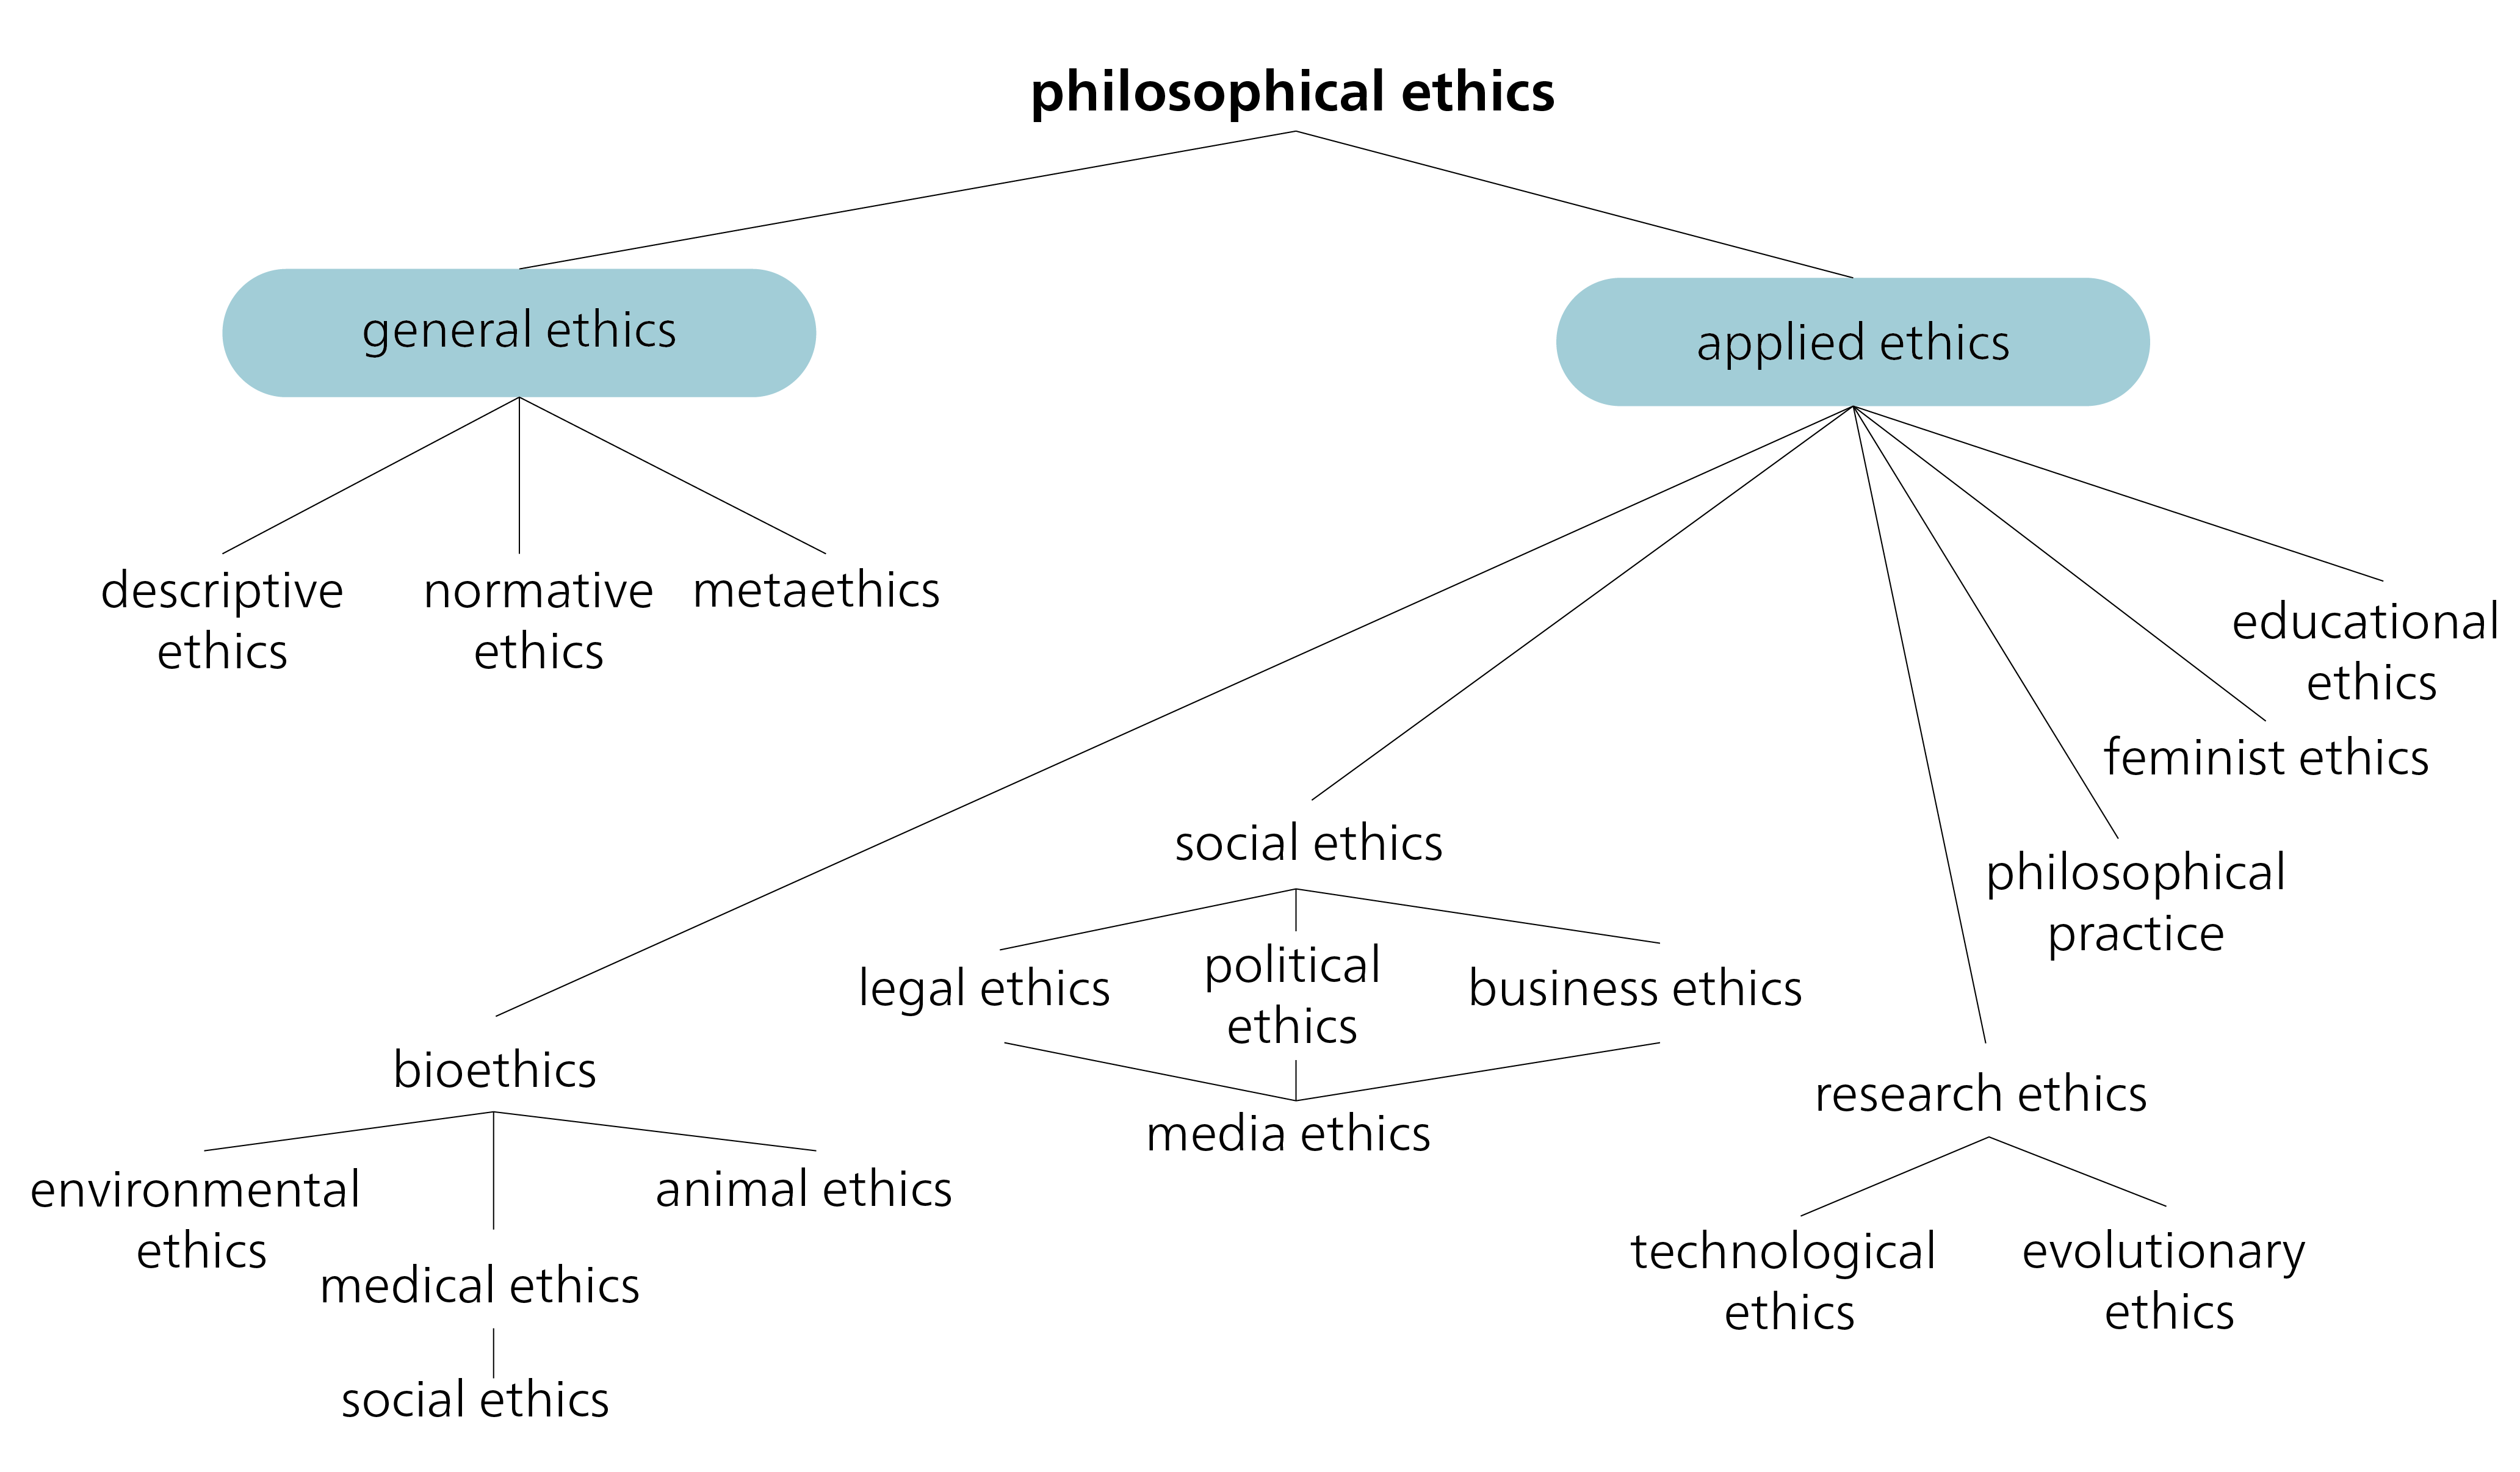
\includegraphics[keepaspectratio]{1_understanding/images/Fig1_7_EthicsBranches.png}}

}

\caption{\label{fig-branches-ethics}The different branches of
philosophical ethics. Source: Own illustration based on Pieper and
Thurnherr 1998: 9.}

\end{figure}%

General ethics provides us with methods and concepts to discuss
fundamental moral problems. It consists of three branches: normative
ethics, descriptive ethics, and metaethics. Normative ethics focuses on
determining what is morally right or wrong. For example, questions about
what constitutes a good life can have different answers, depending on
people's individual values.

For this reason, normative ethics is further divided into teleological
and deontological approaches. Teleological ethics (rooted in telos, the
Greek word for ``end'', ``purpose'', or ``goal'') evaluates actions
based on the good they produce. Utilitarianism, for example, is a
teleological theory that evaluates actions based on the resulting
utility or happiness. One of the first systematic elaborations of
utilitarianism is Jeremy Bentham's (1748--1832) An Introduction to the
Principles of Morals and Legislation (1780). Deontological ethics, on
the other hand, evaluates actions on the basis of their characteristics
rather than their consequences. Its root is deon, Greek for ``duty''. An
example of a deontological ethical theory is Kantian ethics, developed
by the German philosopher Immanuel Kant.

The distinction between teleological and deontological approaches is
often discussed using the ``trolley problem'' (see Sandel {[}2009;
2013{]} for further reading).

\begin{tcolorbox}[enhanced jigsaw, left=2mm, arc=.35mm, titlerule=0mm, opacityback=0, leftrule=.75mm, title={Further reading}, breakable, bottomtitle=1mm, rightrule=.15mm, coltitle=black, toptitle=1mm, bottomrule=.15mm, colback=white, opacitybacktitle=0.6, colbacktitle=quarto-callout-note-color!10!white, toprule=.15mm, colframe=quarto-callout-note-color-frame]

\emph{Justice: What's The Right Thing To Do? Episode 01 ``THE MORAL SIDE
OF MURDER.''} 2009. With Michael Sandel. The Moral Side of Murder.
\url{https://www.youtube.com/watch?v=kBdfcR-8hEY}.

Sandel, Michael. 2013. \emph{Gerechtigkeit.} Ullstein.

\end{tcolorbox}

\subsection{The imperative of responsibility -- Hans
Jonas}\label{the-imperative-of-responsibility-hans-jonas}

Hans Jonas's ``imperative of responsibility'' (1979) offers an important
contribution to the sustainability debate by emphasizing our ethical
responsibility for future generations and for nature. Jonas's approach,
which has been described as a kind of ``ethics of the future'', aims to
address the new challenges posed specifically by a technological
civilization. The link to sustainability ethics lies in his
understanding of the concept of ethical responsibility towards future
generations, which he views as an asymmetric, non-reciprocal
relationship (Jonas 1987a, p.~177). The asymmetry is derived from the
power of a ``moral subject'' over someone or something that requires
care; Jonas describes the vulnerability of life (ontological
vulnerability) and responsibility as our duty of care to protect other
beings from harm (Jonas 1987a, p.~391).

Jonas's approach differs from other ethical theories in that it doesn't
take the existence of humanity for granted, and instead includes duties
towards future generations as well as to nature. Jonas argues that the
first duty of ethics of the future consists in recognizing the distant
effects of human action (Jonas 1987a, p.~64). Given the uncertainty
about the long-term consequences of human action, he proposes a
decision-making principle based on the Latin term, in dubio pro malo,
which he interprets to mean: ``{[}\ldots{]} when in doubt, give the
worse prognosis precedence over the better, as the stakes have become
too high for the game'' (Jonas 1987b, p.~67). Jonas thus develops a new
categorical imperative, emphasizing the need to preserve both nature and
humanity. It is based on the idea that nature has inherent value and
purpose: ``Act in such a way that the effects of your action are
contractual with the permanence of genuine human life on earth'', or
``Act in such a way that the effects of your action are not destructive
to the future possibilities of such life'' (Jonas 1987a, p.~36).

Already in the late 1970s, therefore, Hans Jonas articulated a
fundamental uncertainty about the risks and harm that could arise for
future generations from the technologies that were being used, such as
nuclear energy. Decision-making around issues such as new technologies
requires a continuous evaluation of risks and opportunities, often amid
incomplete information and uncertain future forecasts. These choices not
only impact the environment, but also raise ethical questions about our
obligation to ensure sustainability for future generations. Jonas's
imperative of responsibility emphasizes the link between responsibility
and duty as key concepts in the sustainability debate. According to
Jonas, current generations have a forward-looking responsibility to
future generations. He leaves open, however, the extent of this duty,
and whether future generations are entitled to absolute or comparative
standards.

Jonas's imperative of responsibility can be considered in connection
with various areas of responsibility that represent different ethical
approaches: anthropocentrism, pathocentrism, biocentrism, and
physiocentrism.

\begin{figure}[H]

\centering{

\pandocbounded{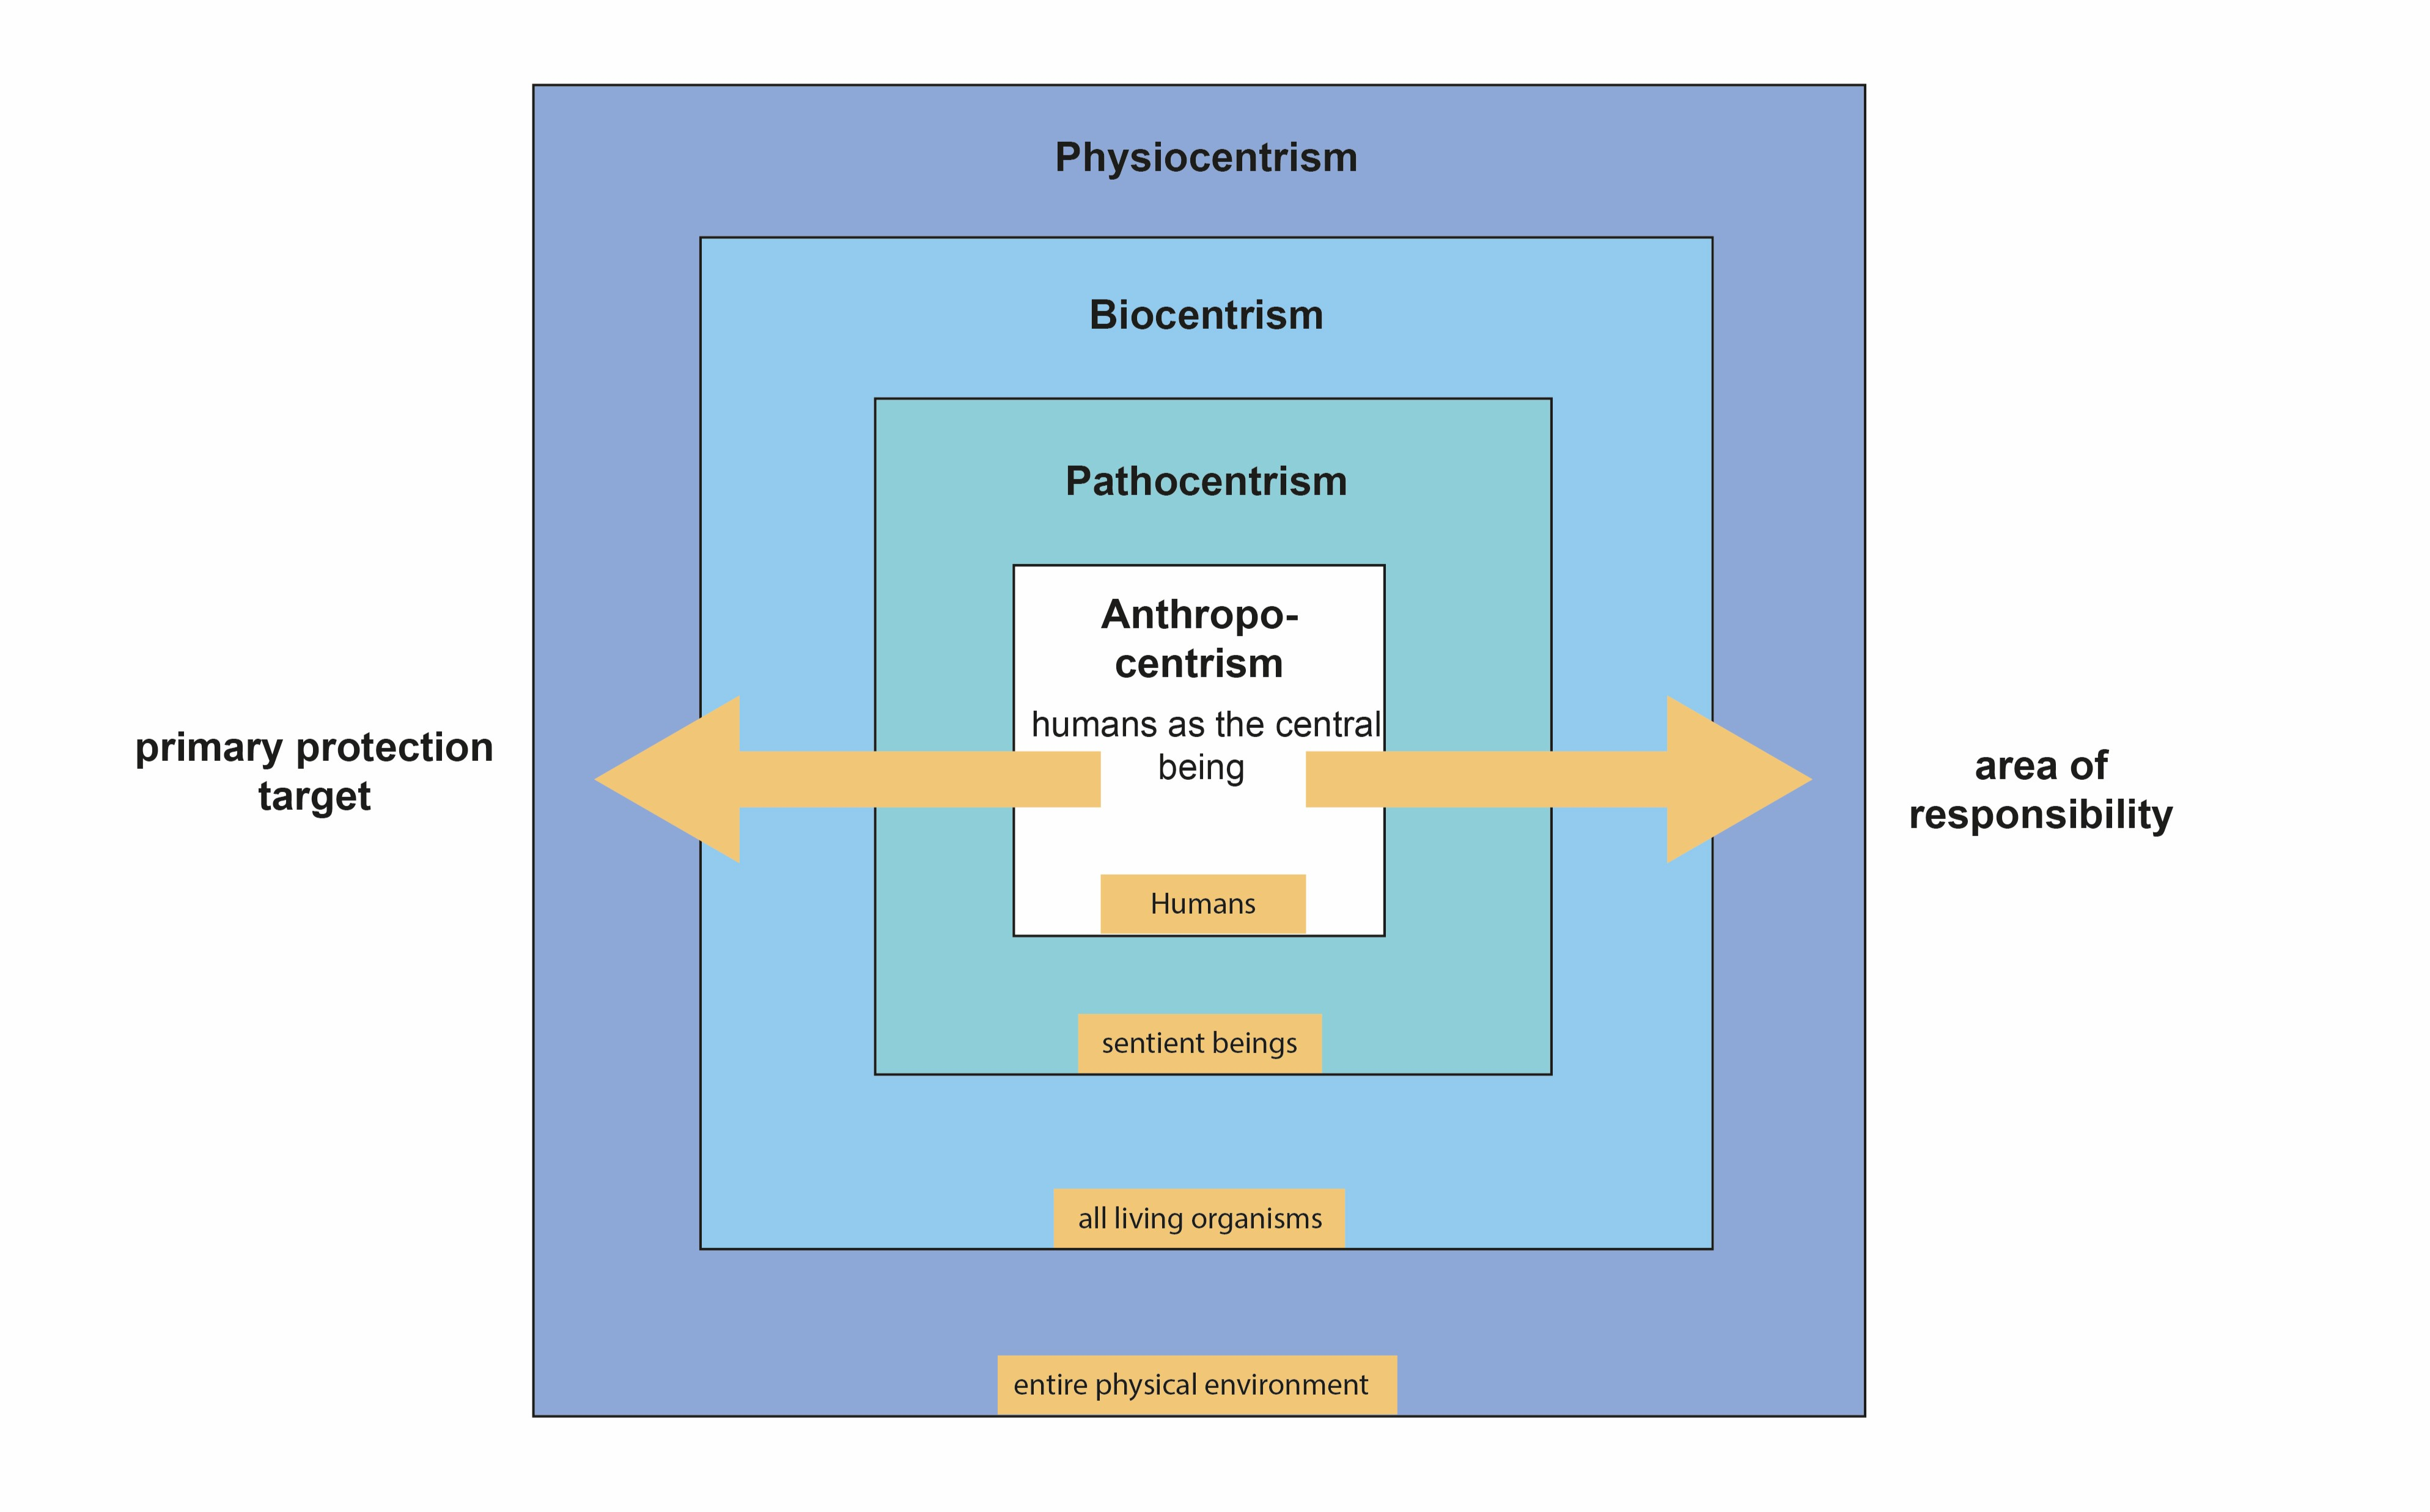
\includegraphics[keepaspectratio]{1_understanding/images/Anthropocentrism.jpg}}

}

\caption{\label{fig-anthropocentrism}Different ethical approaches.
Source: Own illustration based on Carnau 2011: 143.}

\end{figure}%

Anthropocentrism views humans as the central beings, emphasizing
responsibility towards human society and its well-being. This includes
considering the needs and interests of both present and future
generations. Pathocentrism, on the other hand, emphasizes responsibility
towards sentient beings and their well-being. It recognizes that not
only humans, but also animals and other living beings, have the right to
be free from suffering and harm. Biocentrism, in turn, recognizes the
intrinsic value of all living organisms and focuses on the protection
and preservation of biodiversity. It emphasizes the importance of
respecting the natural environment and promoting sustainable practices.
Finally, physiocentrism focuses on the responsibility towards the entire
physical environment, including inanimate nature and ecosystems. It
recognizes the intrinsic value of nature and emphasizes the complex
interactions between all components of the ecosystem.

Hans Jonas's imperative of responsibility reconciles all of these
different areas of responsibility. It urges us to take responsibility
for people as well as for other living beings, nature, and the
environment. In doing so, it is important to adopt a balanced and
comprehensive perspective that takes into account long-term effects and
the well-being of all.

By integrating these different areas of responsibility, we can cultivate
a holistic and sustainable ethic that takes due account of the needs and
interests of all aspects of life and nature.

\section{Sustainable Development in the context of development
debates}\label{sustainable-development-in-the-context-of-development-debates}

Is ``sustainable development'' a development theory? Yes and no. No,
because sustainable development is a broader social model and acts as an
overarching framework that encompasses various development theories.
Yes, because sustainable development is a normative theory that de facto
competes in scientific and social practice with other theories of social
and, in particular, socio-economic development.

Development theories analyse social development, either retrospectively
or prospectively, and either as a whole or through specific aspects
(e.g.~economic development). The retrospective study of social
development seeks to explain past or current social developments and to
draw lessons for future planning and development policy. The prospective
study of social development aims to inform social development management
and policy. Development theories can be categorized into different
types: normative, strategic, and explanatory theories. Each type focuses
on different aspects and objectives of development research.

Normative theories focus on the question of what development should look
like, and what normative goals it should achieve. They examine values
and goals associated with development, often referring to concepts such
as social justice, sustainability, or poverty alleviation. Normative
theories emphasize the definition of criteria for good development, and
provide a normative framework for policy decisions and measures.
Examples include the theory of sustainable development, John Rawls's
theory of social justice, or Amartya Sens's Capability approach.

Strategic theories investigate which strategies and measures are needed
to achieve desired development outcomes. They focus on questions of
policy design, resource allocation, and the implementation of measures,
analysing how specific approaches, such as neoclassical growth theory,
can promote development.

Explanatory theories aim to explain the causes and mechanisms of
development. They analyse factors that drive development processes in
societies and study the links between the different variables. This
involves examining economic, social, political, or cultural factors to
identify patterns and connections. Examples include modernization theory
and dependency theory.

Note: All theories are based on normative foundations -- i.e.~underlying
values and beliefs -- and therefore imply, even unintentionally, certain
ideas about how society should develop.

\begin{longtable}[]{@{}
  >{\raggedright\arraybackslash}p{(\linewidth - 10\tabcolsep) * \real{0.0215}}
  >{\raggedright\arraybackslash}p{(\linewidth - 10\tabcolsep) * \real{0.2432}}
  >{\raggedright\arraybackslash}p{(\linewidth - 10\tabcolsep) * \real{0.0995}}
  >{\raggedright\arraybackslash}p{(\linewidth - 10\tabcolsep) * \real{0.2081}}
  >{\raggedright\arraybackslash}p{(\linewidth - 10\tabcolsep) * \real{0.2161}}
  >{\raggedright\arraybackslash}p{(\linewidth - 10\tabcolsep) * \real{0.2070}}@{}}
\caption{Overview of Development Debates. Source: Extended table based
on Egli et al.~(2022),
p.~378}\label{tbl-development-debates}\tabularnewline
\toprule\noalign{}
\begin{minipage}[b]{\linewidth}\raggedright
\end{minipage} & \begin{minipage}[b]{\linewidth}\raggedright
\textbf{1950s/60s}
\end{minipage} & \begin{minipage}[b]{\linewidth}\raggedright
\textbf{1970s}
\end{minipage} & \begin{minipage}[b]{\linewidth}\raggedright
\textbf{1980s}
\end{minipage} & \begin{minipage}[b]{\linewidth}\raggedright
\textbf{1990s}
\end{minipage} & \begin{minipage}[b]{\linewidth}\raggedright
\textbf{Since 2008}
\end{minipage} \\
\midrule\noalign{}
\endfirsthead
\toprule\noalign{}
\begin{minipage}[b]{\linewidth}\raggedright
\end{minipage} & \begin{minipage}[b]{\linewidth}\raggedright
\textbf{1950s/60s}
\end{minipage} & \begin{minipage}[b]{\linewidth}\raggedright
\textbf{1970s}
\end{minipage} & \begin{minipage}[b]{\linewidth}\raggedright
\textbf{1980s}
\end{minipage} & \begin{minipage}[b]{\linewidth}\raggedright
\textbf{1990s}
\end{minipage} & \begin{minipage}[b]{\linewidth}\raggedright
\textbf{Since 2008}
\end{minipage} \\
\midrule\noalign{}
\endhead
\bottomrule\noalign{}
\endlastfoot
\textbf{Narrative} & Economic growth, modernization, and integration
into the world economy & Fight against extreme poverty and inequality &
Lost decade: collapse of commodity prices; increase in debt &
Sustainable development; decade of hope & Polycrisis \\
\textbf{Basic idea} & Catch-up development through industrialization and
large-scale projects & Satisfaction of basic needs, growth, and
effective distribution & Overcoming the debt crisis through structural
adjustment measures, reduction of state services & Global and
sustainable environmental policy, economic growth, peacekeeping,
continuing basic needs strategy, participation & Bringing together
various crisis phenomena (financial crisis, climate change, biodiversity
crisis, etc.) and examining their complex interrelations; search for
integrated solutions \\
\textbf{Theories} & Modernization theories (stage theories) & Dependency
theories versus modernization theories & Market liberalism and
neoliberalism & - Theories of sustainable development - Neoclassical
growth theory - Postcolonial theories - Capability approach -
Post-development theories & Additional resilience theories, post-growth
theories \\
\textbf{Goals} & Geopolitical classification of the ``Third World'';
containment of communism, modernization of agriculture, rapid
industrialization and technological progress, opening up of new markets
& Aid for self-help, appropriate technologies, rural development,
promotion of women & Increase in exports, balanced state budgets &
Paradigm shift in development aid towards development cooperation,
environmental and social compatibility of development, ensuring access
to resources and infrastructure for all & \\
\textbf{Consequences} & Economic dependence and indebtedness increase,
income disparities widen, poverty rises, ecological damage due to
overuse and inappropriate technologies, undemocratic regimes are
supported for geopolitical reasons & Selective progress in education and
health, problems of debt and environmental damage & Living standards of
the poorest population groups deteriorate severely, environmental
exploitation, debt spiral, increase of dependency of the Global South on
Global North countries & Focus shifts from purely economic development
to human development; industrialized countries are obliged to implement
sustainable development; emergence of a global development partnership
& \\
\end{longtable}

\begin{tcolorbox}[enhanced jigsaw, left=2mm, arc=.35mm, titlerule=0mm, opacityback=0, leftrule=.75mm, title={Development theories}, breakable, bottomtitle=1mm, rightrule=.15mm, coltitle=black, toptitle=1mm, bottomrule=.15mm, colback=white, opacitybacktitle=0.6, colbacktitle=quarto-callout-note-color!10!white, toprule=.15mm, colframe=quarto-callout-note-color-frame]

\textbf{Modernization theory} (1950s--1980s) emphasizes the transition
from traditional societies to modern, industrialized societies as the
basis for development. For proponents of modernization theory, the
countries of the Global South are developing in the same direction as
industrialized countries, but at a much slower pace. Modernization
theory values economic growth, technological progress, and institutional
adjustments. It is often associated with stage theories, which emerged
in the 1950s and 1960s. Stage theories view development as a gradual
process characterized by clearly defined stages or phases of
development, with emphasis on economic growth and modernization.
Prominent proponents include Walt Rostow, who identified five stages of
development in his work, The Stages of Economic Growth: A Non-Communist
Manifesto (i.e.~traditional society, preconditions for take-off,
take-off, drive to maturity, and mass consumption).

\textbf{Dependency theory} (1970s and 1980s) emphasizes the structural
dependence and inequality between developed and developing countries. It
argues that developing countries are trapped in an unjust global
economic system and remain dependent on developed countries.

\textbf{Neoclassical growth theory} (as of the 1990s) focuses on the
connection between capital accumulation, technological progress, and
economic growth. It emphasizes free markets, trade, and investment as
drivers of development.

\textbf{Postcolonial theories} (as of the 1990s) emphasize the
historical and structural inequality between former colonial powers and
colonies. They argue that development can only be achieved through a
critical examination of the legacy of colonialism.

\textbf{Sen's Capability approach} (as of the 1990s) emphasizes the
importance of freedom, social justice, and human development. It
emphasizes the necessity to improve the opportunities and capabilities
of people in order to achieve development.

\textbf{Post-development theories} (as of the 1990s) criticize linear
development models that impose Western ideas of progress, emphasizing
instead local practices and values. Prominent thinkers in this field
include Arturo Escobar, who critically reflects on the idea of
development in his work Encountering Development: The Making and
Unmaking of the Third World, and Vandana Shiva, whose Decolonizing the
North calls for a sustainable and fairer development policy in the
Global South that reduces the influence of the Global North.

\end{tcolorbox}

\section{Sustainability models}\label{sustainability-models}

\subsection{Three dimensions of
sustainability}\label{three-dimensions-of-sustainability}

The established three-sector model of sustainability, introduced in the
1987 Brundtland Report, s eeks to balance environmental, economic, and
social concerns. This model, which later also became known as the
``triple bottom line'' model, emphasized that economic development
should be profitable while ensuring that environmental and social
impacts remain neutral. On closer inspection, however, the model --
initially depicted as a building with three pillars -- has a major
weakness. While it was intended to suggest that if any one pillar was
weak, the system as a whole would be unsustainable - it could be argued
that removing one of the pillars -- or even the two outer pillars --
would not make the building collapse if the remaining pillar(s) were
strong enough. Despite its widespread use and overall success, the model
struggles with transparency and equity. For example, measuring economic
success requires quantitative indicators, while it's hard to find
similar metrics for social well-being, especially emotional aspects.
Some critics argue that the model prioritizes conventional economic
thinking, neglecting important social aspects. An overemphasis on human
economic systems can also prevent us from seeing our dependence on
non-human ecological systems.

\subsection{Sustainability as an
intersection}\label{sustainability-as-an-intersection}

\begin{figure}[H]

\centering{

\pandocbounded{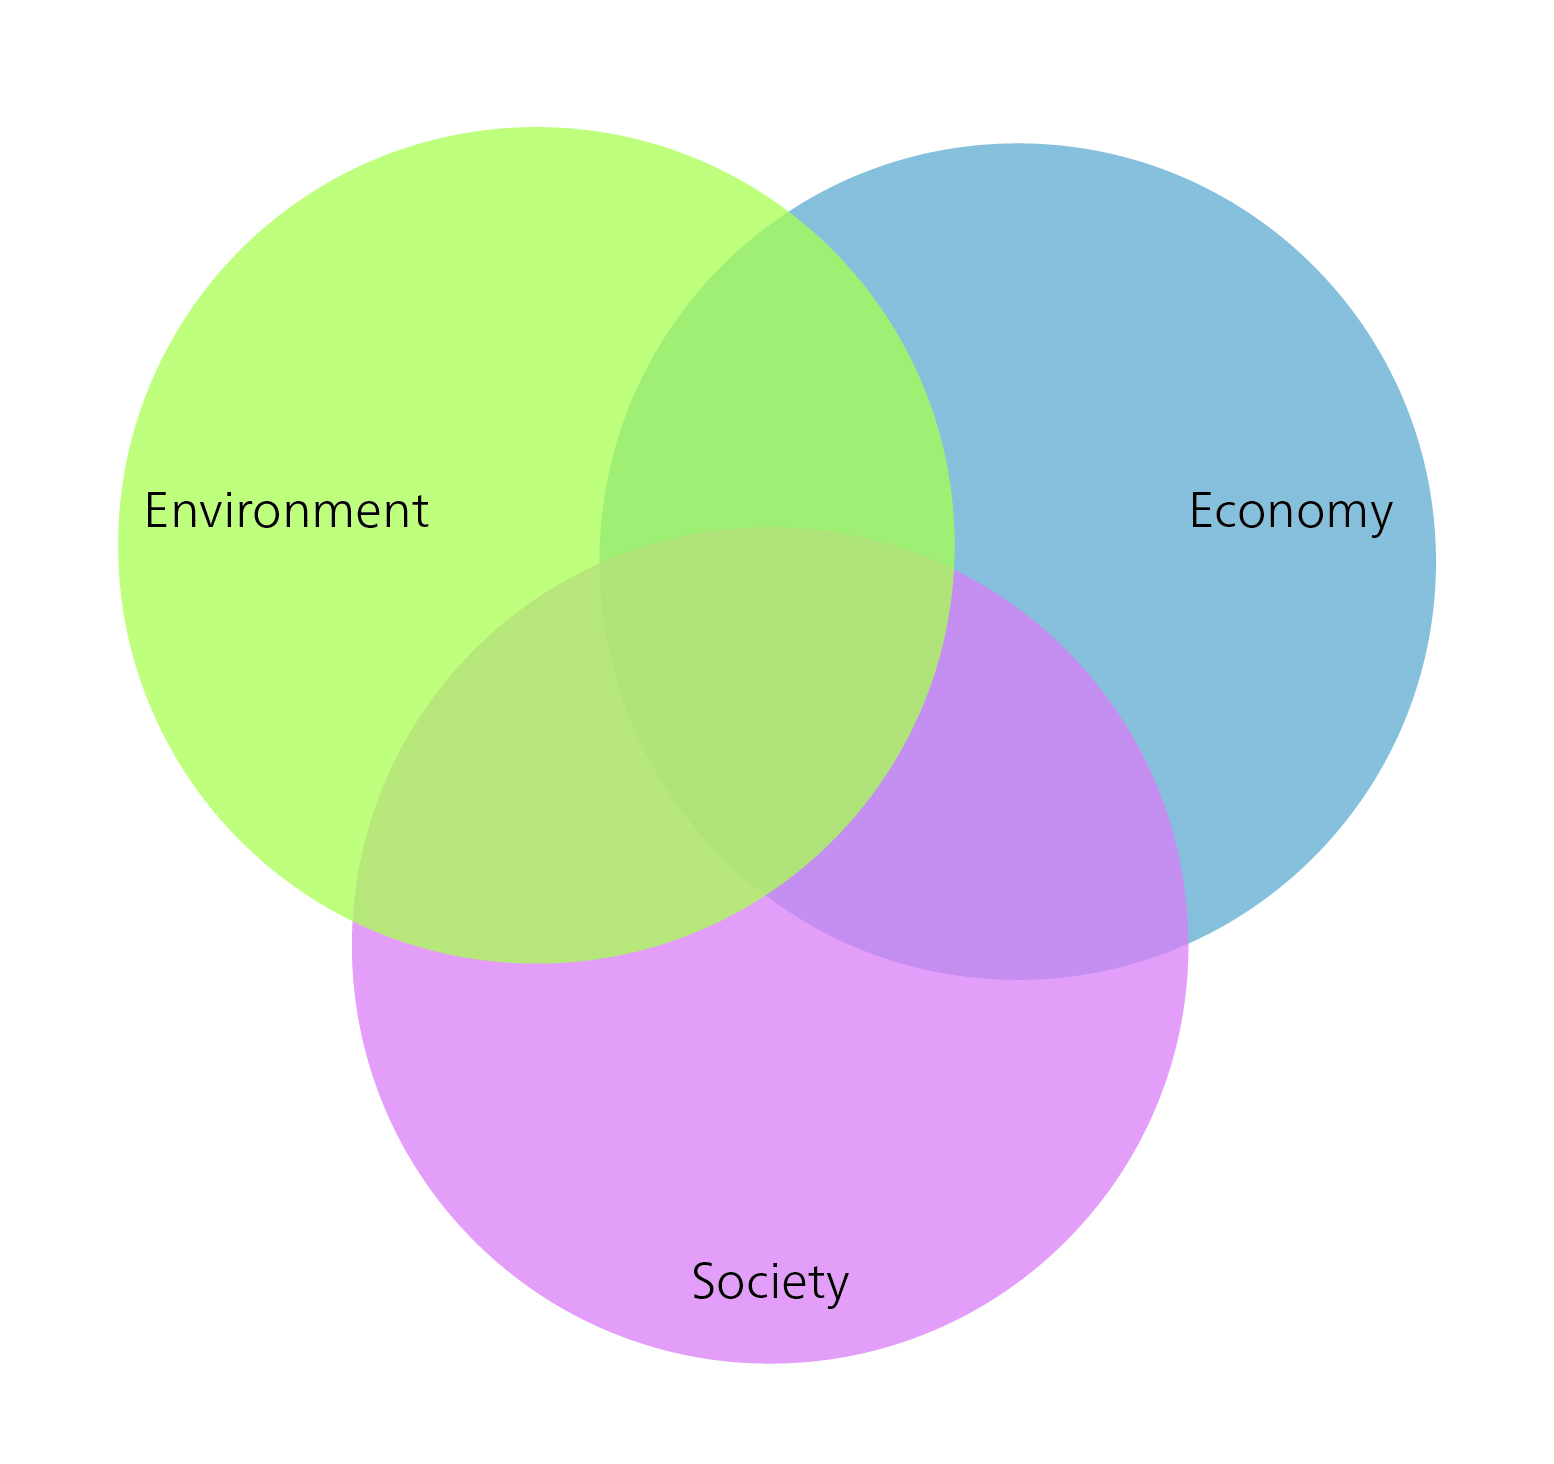
\includegraphics[keepaspectratio]{1_understanding/images/sustainability-intersection.jpg}}

}

\caption{\label{fig-sustainability-intersection}Sustainability as an
intersection. Source: Own illustration.}

\end{figure}%

A model displaying the three sectors as a Venn diagram (overlapping
rings or circles, sometimes known as the intersection or triad model)
offers an alternative to the separate pillars, emphasizing the
interconnectedness of the three dimensions. This model illustrates that
there can be a closer connection between two areas, and that the
boundaries are fluid.

\subsection{Nested sustainable
development}\label{nested-sustainable-development}

Giddings et al.~(2002) challenge the idea of separate spheres for the
economy, society, and environment. They propose a ``nested'' model,
where the economy is seen as part of society, which in turn is embedded
in the environment. This model, they argue, ensures that economic
decisions are always constrained by social and environmental factors.
Global ecosystems form the basis for social systems (i.e.~society).
Embedded therein is the economy, which serves society's needs. A
potential drawback of this model, however, is that if the economy is the
starting point for all sustainability considerations, there's a risk of
prioritizing it over social and environmental considerations.¨

\begin{figure}[H]

\centering{

\pandocbounded{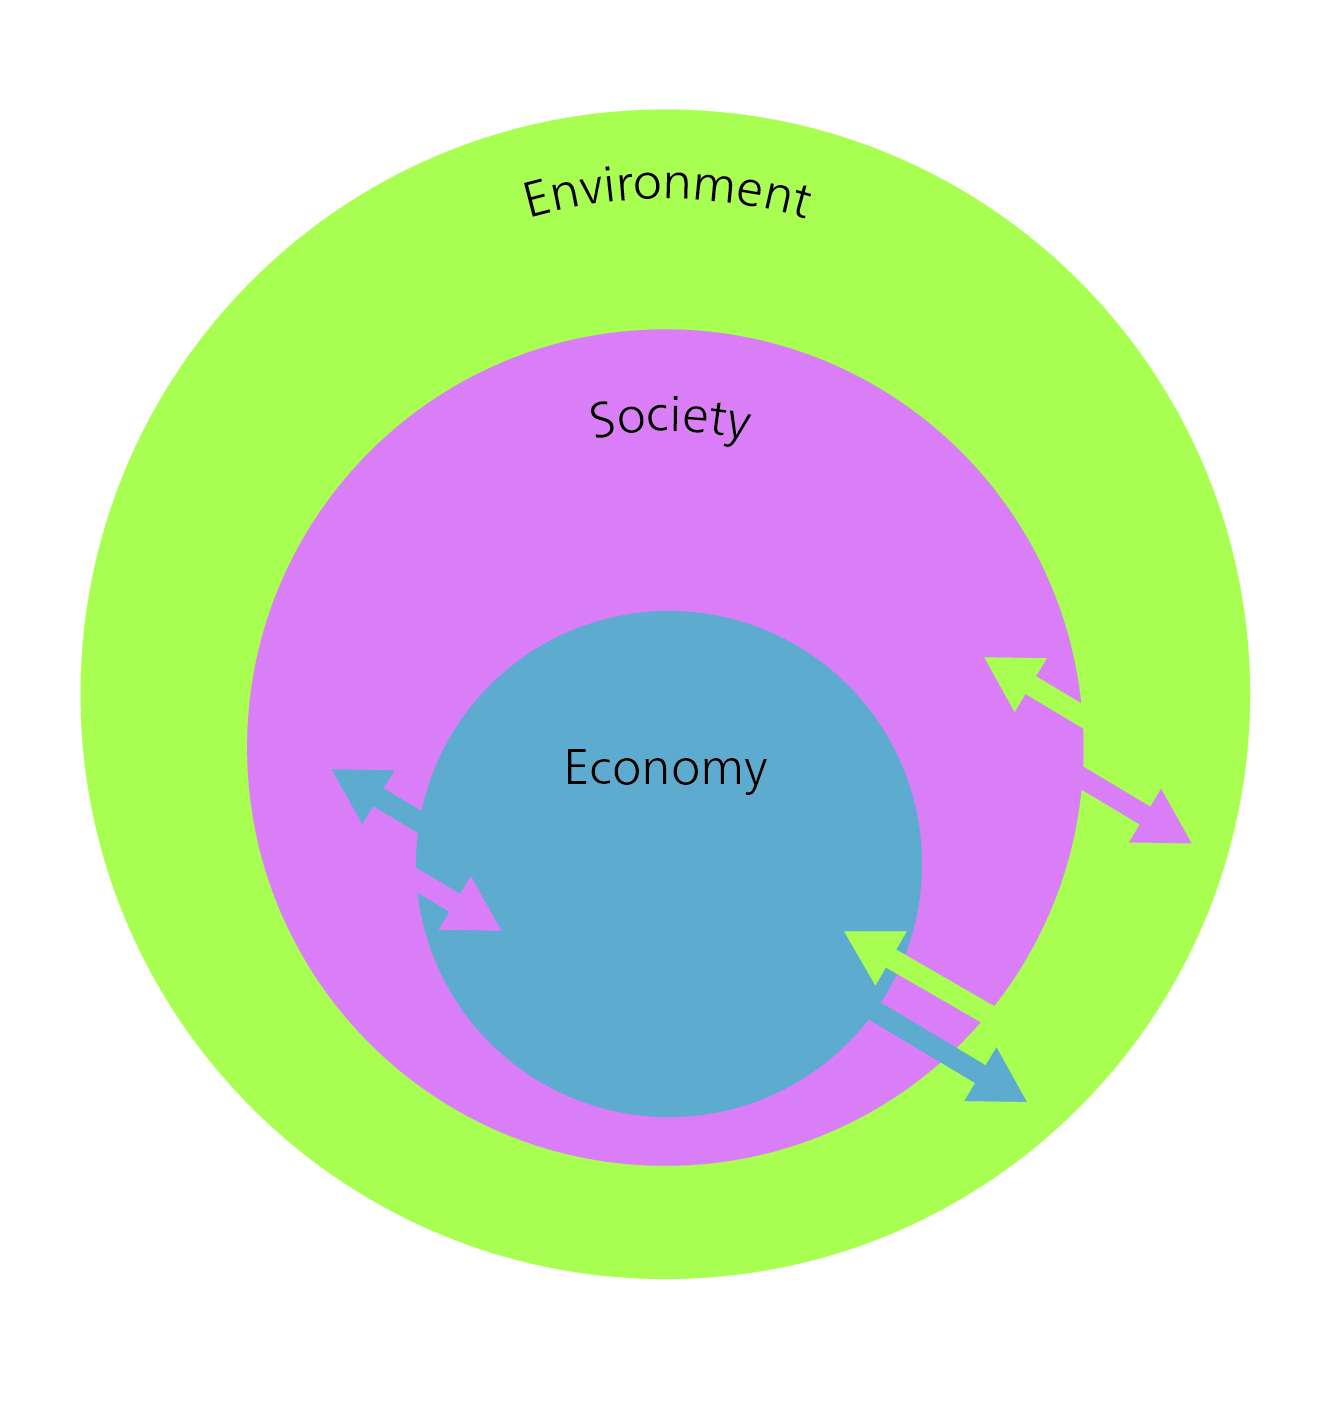
\includegraphics[keepaspectratio]{1_understanding/images/sustainability-nested.jpg}}

}

\caption{\label{fig-sustainability-nested}The nested model of
sustainability. Source: Own illustration adapted from Giddings (2002:
192).}

\end{figure}%

\subsection{A four-dimensional model of
sustainability}\label{a-four-dimensional-model-of-sustainability}

One problem with the three-sector model of sustainability is that that
it's unclear what falls within the broad ``social'' sphere. It has
therefore been suggested that a fourth dimension be added, to emphasize
certain aspects that might otherwise remain hidden in the social sector.
For example, Jon Hawkes, an Australian cultural commentator , has
suggested adding ``cultural vitality'' as a fourth pillar of
sustainability, in addition to environmental, economic, and social
concerns.

\begin{figure}[H]

\centering{

\pandocbounded{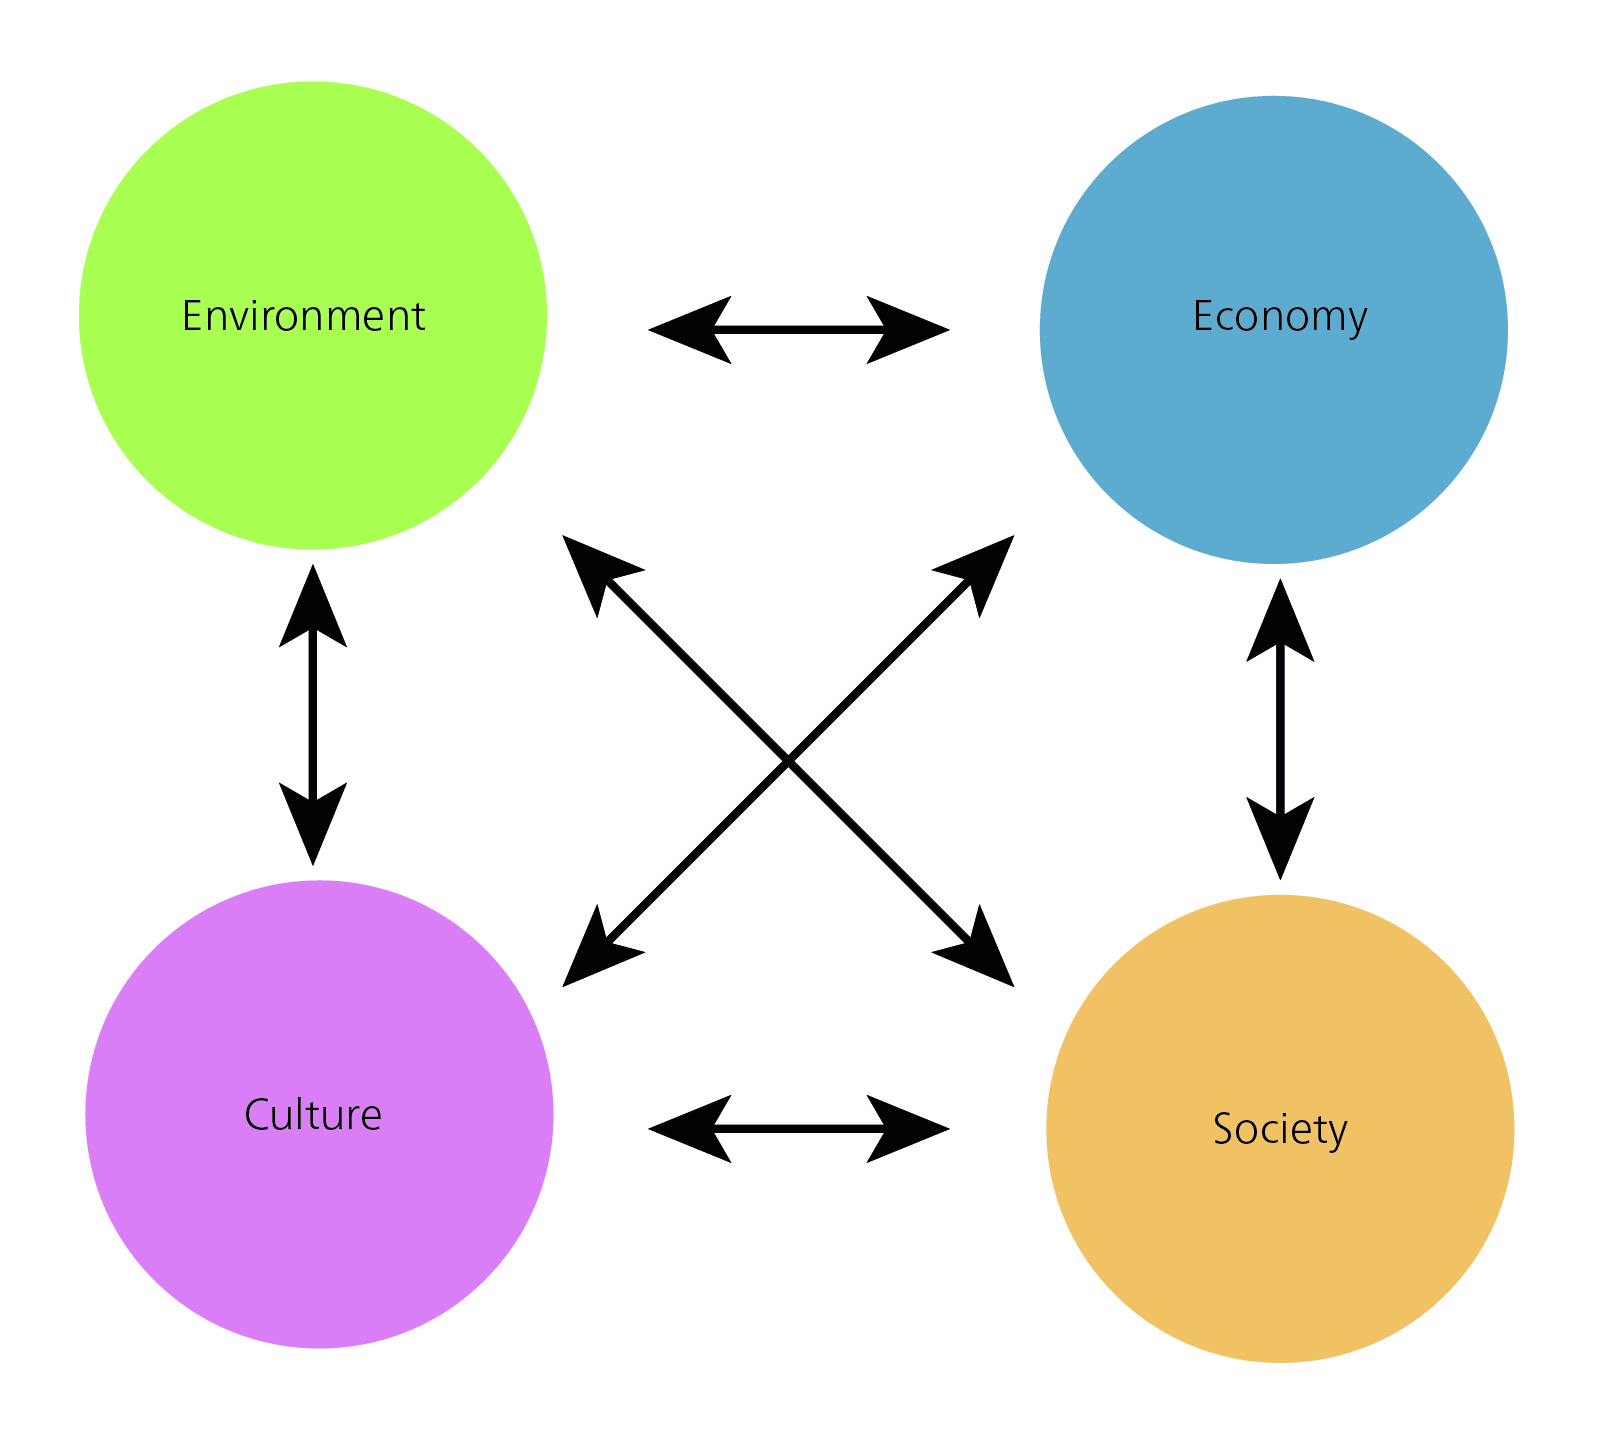
\includegraphics[keepaspectratio]{1_understanding/images/sustainability-4-dimensions.jpg}}

}

\caption{\label{fig-sustainability-4-dimensions}Four-dimensional model
of sustainability. Source: Own illustration, adapted from Hawkes, 2004.}

\end{figure}%

Cultural sustainability is often seen as a part of social
sustainability. Sometimes the term ``sociocultural sustainability'' is
also used. In this context, ``culture'' refers to aspects such as
equity, opportunities for participation, awareness of sustainability,
and general operating and behavioural models (Murphy, 2017). It's clear
that the social and cultural dimensions are closely linked. Cultural
processes influence our social lives and how we view social
sustainability, like the value we place on equality as a social goal. In
turn, social structures and institutions influence cultural practices
and judgements. Despite this strong connection, cultural and social
sustainability can also be seen as separate dimensions or perspectives
of sustainability.

Culture does not have its own Sustainable Development Goal (SDG). In the
2030 Agenda, culture is mentioned in relation to ``civilization'',
``diversity'', ``interculturality'', ``cultural heritage'', and
``tourism'', under the following four SDGs: quality education (SDG 4),
decent work and economic growth (SDG 8), sustainable cities and
communities (SDG 11), and responsible consumption and production (SDG
12) (Duxbury et al., 2017).

The concept of cultural sustainability can be interpreted in different
ways: as the fourth dimension of sustainability, as culture for
sustainability, and as culture as sustainability. The interpretation of
``culture as sustainability'' requires a new way of thinking and a new
paradigm in relation to sustainability. In this view, culture itself is
transformed towards sustainability. Cultural sustainability here means
thinking about what needs to be preserved, what needs to change, and how
we can implement these changes. This interpretation -- viewing culture
as sustainable development -- defines culture in the broadest sense as a
comprehensive lifestyle and a continuously changing process. Our social
order (such as capitalism and democracy), our values, and our ways of
working are all cultural products. Culture thus encompasses all the
other dimensions of sustainability and transforming it becomes a key
concern or paradigm for sustainability.

The definition of cultural sustainability contains several important
aspects: Firstly, it emphasizes the importance of intellectual growth
and responsibility. This means acquiring knowledge, developing a better
understanding of important issues, and participating in educational
activities and events. It also means acting not only as individuals, but
also as members of different communities. All problematic and
unsustainable structures and operating models have been created and
developed by humans. We humans, therefore, also have the opportunity to
change them.

Cultural sustainability is required, for example, for a ``Great
Transformation'' as advocated by Uwe Schneidewind (2018). In his work,
Schneidewind emphasizes the need for comprehensive change in all
dimensions of society, including culture, in order to achieve
sustainable development. Recognizing cultural sustainability as a
central paradigm of sustainability supports the vision of a
comprehensive transformation that goes beyond technological and economic
solutions and strives for a fundamental societal change of course.

\section{Weak and strong
sustainability}\label{weak-and-strong-sustainability}

The academic debate on sustainability distinguishes between weak and
strong sustainability (see e.g.~Ott, 2020). Neither concept can easily
be dismissed, as both rely on assumptions that are difficult to refute.
In practice, both concepts are considered partially true, with evidence
both in favour and against. The key difference between weak and strong
sustainability is the question of what we should sustain, and the degree
to which what forms of capital can be substituted. This concerns, in
particular, the following three forms of capital: natural capital,
manufactured capital , and human capital.

Natural capital: the natural resources and ecosystems that are key to
human well-being and sustainable development. These include land, water,
air, biodiversity, and renewable energy. Natural capital is the basis
for many economic activities, and it provides essential ecosystem
services such as food, the purification of water and air, and cultural
and aesthetic benefits.

Manufactured capital: the material resources and infrastructure used in
production and economic activity. This includes buildings, machinery,
technological equipment, means of transport, and physical
infrastructure. Manufactured capital is closely linked to economic
growth and productivity, and plays an important role in economic
development.

Human capital: the knowledge, skills, level of education, health, and
creative abilities of people in a society. It encompasses individual and
collective knowledge as well as the skills needed for economic
productivity and social progress. Human capital is important for
innovation, labour productivity, social participation, and the ability
of a society to tackle challenges and to adapt.

\subsection{Weak sustainability}\label{weak-sustainability}

Weak sustainability can be considered the ``soft'' or flexible option.
Supporters of weak sustainability believe that an action is sustainable
if it offers an advantage to the overall system, or at least does not
reduce its quality. Weak sustainability can therefore be seen as a basic
requirement of sustainability, in that it aims to maintain a certain
level of well-being/quality of life or to ensure equality. The concept
of weak sustainability ``assumes the extensive and, at least in
principle, unlimited {[}\ldots{]} substitutability of all types of
capital'' (Ott \& Döring, 2004: 41) and is thus based on the premise of
neoclassical economics. Proponents of weak sustainability believe that
natural capital can be substituted with other forms of capital. They
emphasize the concept of ``total capital'', arguing that the specific
make-up of the capital inherited by future generations is irrelevant, as
long as overall benefits and well-being are sustained. This aligns with
neoclassical utility theory, according to which it is irrelevant how
utility is generated.

Weak sustainability supporters therefore believe that measures can be
considered sustainable, even if they are carried out at the expense of
natural capital -- as long as this loss is compensated for by an
increase in human or manufactured capital. This could justify the
extraction of raw materials such as coal or excessive crude oil. And
Carlowitz's Silvicultura oeconomica forest, could, in principle, also be
replaceable or degradable, provided that its natural and cultural
functions can be fulfilled in other ways by future generations. This
understanding of sustainability emphasizes the importance of
technological progress for sustainable development.

Evaluating measures based on weak sustainability is challenging, due to
the inherent complexities and numerous assumptions involved. This goes
beyond fundamental questions about sustainability, such as ``What is a
good life?'', or ``How do we measure the level of well-being?''. A key
challenge lies in assigning a monetary valuation to different types of
capital, especially those lacking a clear market price. To
operationalize this, what factors should be taken into account? What is
the value of natural beauty? What is the value of a rare bird or a
whale? Buller's The Value of a Whale (2022) impressively outlines the
problems we face in trying to put a price on elements of nature.

Critics of the concept of weak sustainability point to several
limitations. Firstly, they question the assumption that natural
resources can be endlessly replaced by reproducible capital. Secondly,
they doubt whether an increase in goods can truly compensate for the
loss of environmental quality. Finally, concerns exist about our ability
to develop new resources and the potential for exceeding critical
threshold values. These criticisms have paved the way for the concept of
``strong sustainability''.

\subsection{Strong sustainability}\label{strong-sustainability}

In contrast to weak sustainability, strong sustainability emphasizes the
preservation of natural capital. Proponents of this eco-centric theory
are less optimistic about our ability to substitute natural resources
with manufactured ones, believing these resource types to have limited
interchangeability (Daly, 1990; 1999; Ott 2001, Ott \& Döring 2004).
They argue that the individual elements of natural capital should be
kept as constant as possible, to prevent, for example, species
extinction.

\begin{longtable}[]{@{}
  >{\raggedright\arraybackslash}p{(\linewidth - 8\tabcolsep) * \real{0.0936}}
  >{\raggedright\arraybackslash}p{(\linewidth - 8\tabcolsep) * \real{0.2456}}
  >{\raggedright\arraybackslash}p{(\linewidth - 8\tabcolsep) * \real{0.2135}}
  >{\raggedright\arraybackslash}p{(\linewidth - 8\tabcolsep) * \real{0.2222}}
  >{\raggedright\arraybackslash}p{(\linewidth - 8\tabcolsep) * \real{0.2164}}@{}}
\caption{Weak and Strong Sustainability. Source: Derived from Eblinghaus
\& Stickler 1998; Dobson 2002; Rieckmann 2004; Steurer 2001; Michelsen
et al.~2016}\tabularnewline
\toprule\noalign{}
\begin{minipage}[b]{\linewidth}\raggedright
\textbf{Category}
\end{minipage} & \begin{minipage}[b]{\linewidth}\raggedright
\textbf{Very Weak Sustainability}
\end{minipage} & \begin{minipage}[b]{\linewidth}\raggedright
\textbf{Weak Sustainability}
\end{minipage} & \begin{minipage}[b]{\linewidth}\raggedright
\textbf{Strong Sustainability}
\end{minipage} & \begin{minipage}[b]{\linewidth}\raggedright
\textbf{Very Strong Sustainability}
\end{minipage} \\
\midrule\noalign{}
\endfirsthead
\toprule\noalign{}
\begin{minipage}[b]{\linewidth}\raggedright
\textbf{Category}
\end{minipage} & \begin{minipage}[b]{\linewidth}\raggedright
\textbf{Very Weak Sustainability}
\end{minipage} & \begin{minipage}[b]{\linewidth}\raggedright
\textbf{Weak Sustainability}
\end{minipage} & \begin{minipage}[b]{\linewidth}\raggedright
\textbf{Strong Sustainability}
\end{minipage} & \begin{minipage}[b]{\linewidth}\raggedright
\textbf{Very Strong Sustainability}
\end{minipage} \\
\midrule\noalign{}
\endhead
\bottomrule\noalign{}
\endlastfoot
\textbf{What should be preserved?} & Total capital & Essential natural
capital & Non-renewable natural capital & Nature has its own value \\
\textbf{Why?} & Maximization of economic profit and individual welfare
(GDP) & + Limitation of environmental damage and resource scarcity &
Ensuring long-term living conditions for humans and nature & + Respect
for all forms of life and duties toward nature \\
\begin{minipage}[t]{\linewidth}\raggedright
\textbf{How?\\
(Policies)}\strut
\end{minipage} & Growth orientation through promotion of technology and
innovation & Environmental regulations, resource efficiency, renewable
energies & + Conservation measures, ecological restoration, sustainable
agriculture & \\
\textbf{Substitutability} & In principle unlimited, natural resources
can be replaced by technology and trade & Partly possible, but limited
substitutability of ecosystem services & Limited, critical threshold for
environmental changes & Low, recognition of unique values and
relationships \\
\textbf{Ethics} & Anthropocentric, short-term benefits take priority &
Anthropocentric with stronger consideration of environmental interests &
Pathocentrism, recognition of intrinsic value of nature & Biocentrism,
ecological integrity, ethical responsibility toward nature \\
\end{longtable}

While neoclassical economists are confident about substitution,
proponents of strong sustainability emphasize the importance of
prevention and anticipation, rather than aftercare and reaction. For
example, reacting to the hole in the ozone layer by using sun cream,
protective clothing, or medical aftercare fails to tackle the cause of
the problem. Similarly, technological approaches such as geo-engineering
are criticized for merely treating problems superficially.
Geo-engineering refers to technical interventions in geochemical or
biogeochemical cycles, for example to slow down climate change or ocean
acidification.

Until now, reducing pollution has mainly focused on end-of-pipe
technologies, such as flue gas cleaning systems on factory chimneys or
catalytic converters in cars. But this also meant that we put off
tackling long-term environmental problems, such as climate change or
biodiversity loss, as long as their effects were not immediately
apparent. This phenomenon is linked to the concept of externalization,
in which environmental and social costs are shifted outwards, as
described by Lessenich (2018). This means that pricing only takes into
account the economic costs, partly because they are easier to quantify,
while the social and environmental costs of providing goods and services
are omitted or externalized, leading to distortions in market prices.

\section{Sustainability strategies as principles of sustainable
development}\label{sustainability-strategies-as-principles-of-sustainable-development}

\begin{figure}[H]

\centering{

\pandocbounded{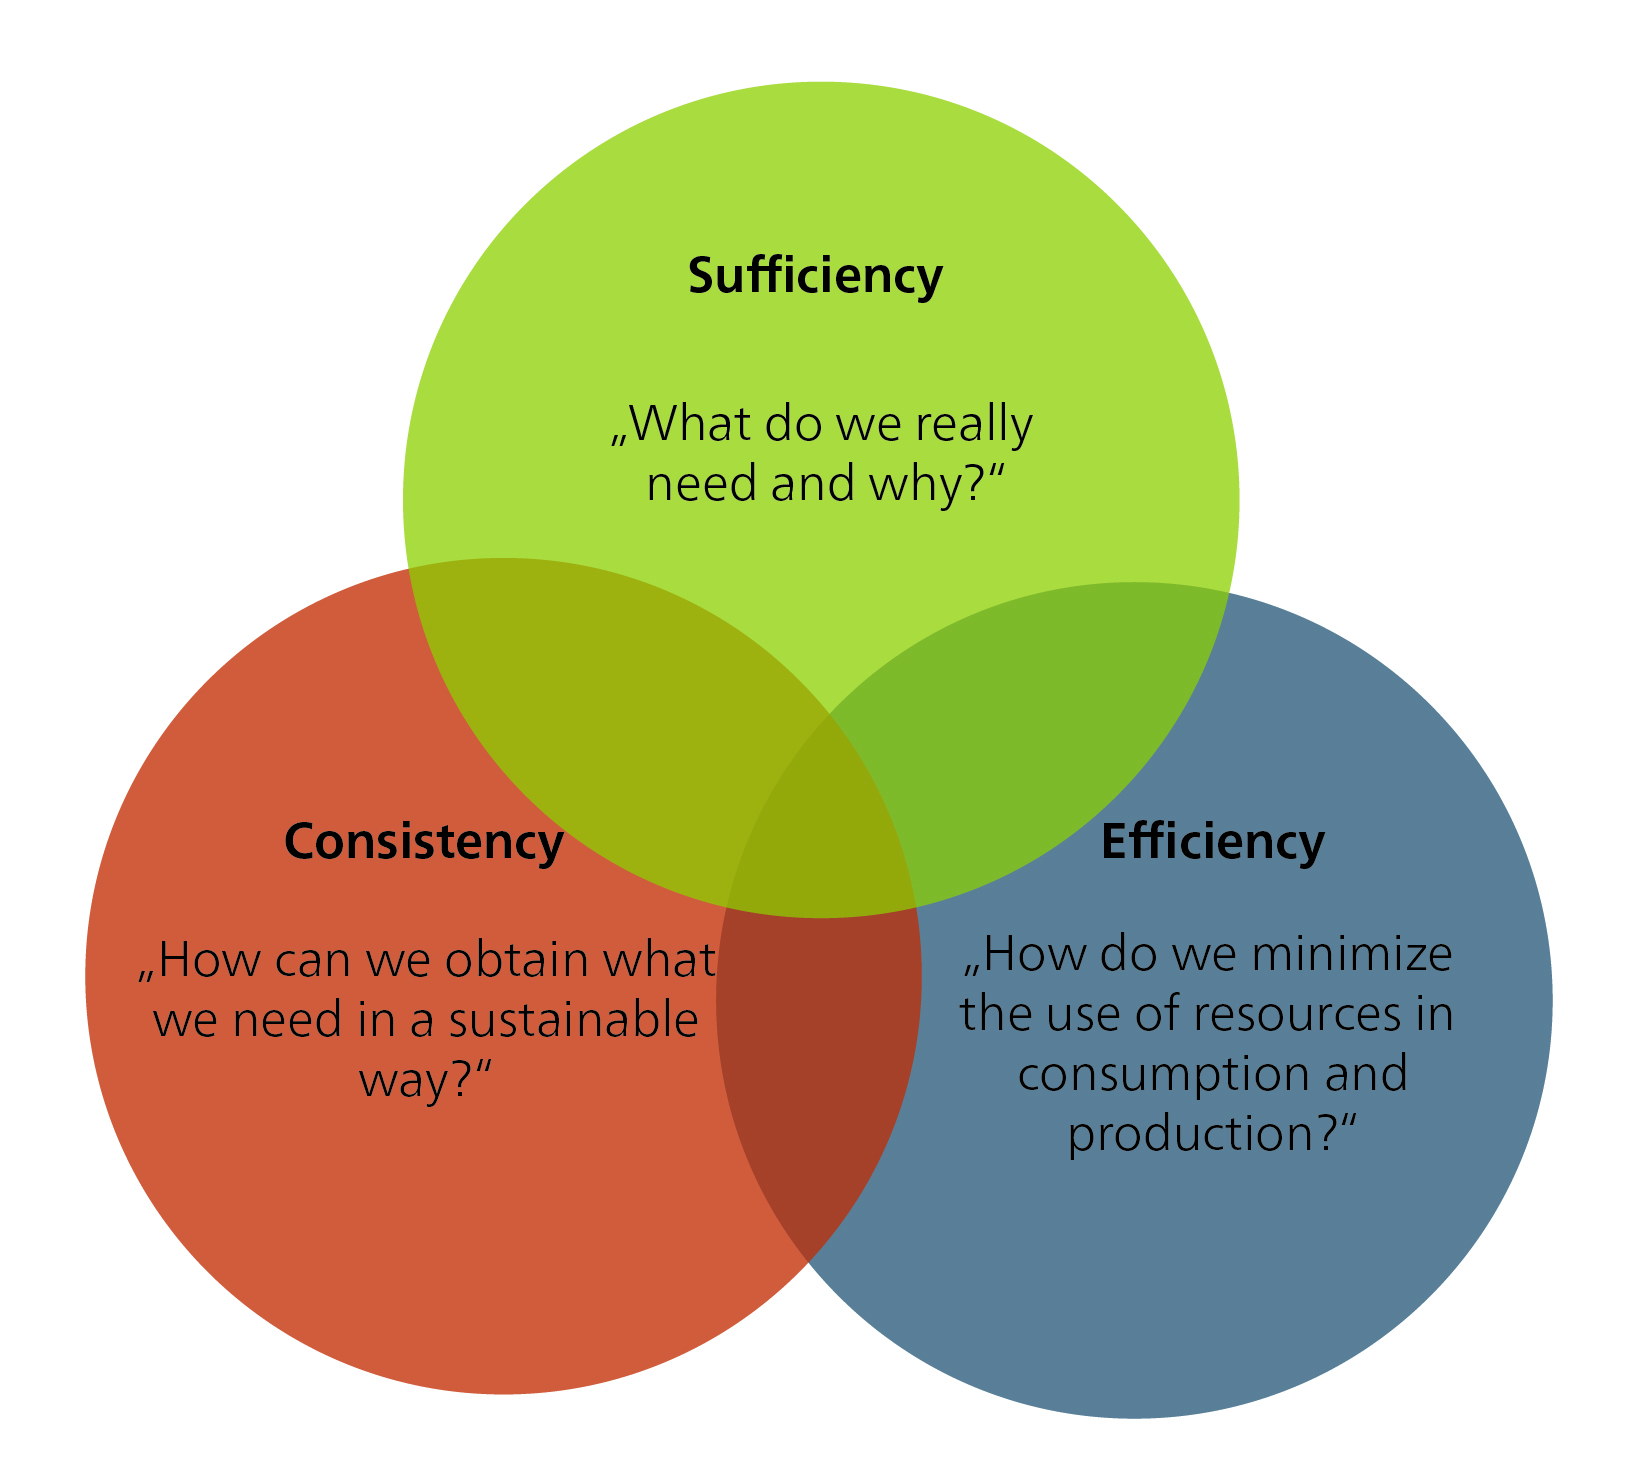
\includegraphics[keepaspectratio]{1_understanding/images/sustainability-strategies.jpg}}

}

\caption{\label{fig-sustainability-strategies}Sustainability strategies
(Own illustration).}

\end{figure}%

\subsection{Efficiency strategy}\label{efficiency-strategy}

The efficiency strategy focuses on minimizing resource use (i.e.~raw
materials and energy) in manufacturing or service provision. This
translates to reducing material consumption (material intensity), energy
consumption (energy intensity), and emissions of harmful substances such
as CO2. Also known as ``eco-efficiency'', this strategy is attractive to
business and society, as it can reduce costs, resource use, and
environmental impact. Implementing the efficiency strategy starts with
improving production processes, primarily through technological
advancements. Proponents believe it's possible to double prosperity
while halving natural resource use (Weizsäcker et al.~1995). However,
critics of the efficiency strategy are less optimistic, and caution
against overestimating its impact on sustainable economic activity. They
point to ``rebound effects'', which can reduce or even wipe out the
gains from efficiency increases (Paech 2012; Santarius 2014 ).

\begin{tcolorbox}[enhanced jigsaw, left=2mm, arc=.35mm, titlerule=0mm, opacityback=0, leftrule=.75mm, title={Putting Efficiency Strategies into Action: Examples}, breakable, bottomtitle=1mm, rightrule=.15mm, coltitle=black, toptitle=1mm, bottomrule=.15mm, colback=white, opacitybacktitle=0.6, colbacktitle=quarto-callout-tip-color!10!white, toprule=.15mm, colframe=quarto-callout-tip-color-frame]

\textbf{Energy-efficient lighting}: Replacing conventional lightbulbs
with energy-efficient LED bulbs lowers electricity use and helps reduce
the demand for energy.

\textbf{Fuel-efficient vehicles}: The development of more fuel-efficient
hybrid or electric vehicles can lead to lower fuel consumption and road
transport emissions.

\textbf{Efficient building technology}: Installing smart HVAC (heating,
ventilation, and air conditioning) systems in buildings helps to reduce
energy consumption for heating and cooling.

\textbf{Efficient water use}: The use of water-saving fittings and
systems in households and industrial companies reduces water consumption
and minimizes waste.

\end{tcolorbox}

\subsection{Consistency strategy}\label{consistency-strategy}

While the efficiency strategy focuses on quantity (reducing resource use
while achieving greater output), the consistency strategy (from the
Latin con = together + sistere = to stop ) strives to reconcile nature
and technology by using resources repeatedly instead of only once.
Instead of fossil fuel-based resources, products, and technologies, it
seeks to use materials that are compatible with natural material cycles
and processes. Also referred to as ``eco-effectiveness'', this concept
follows the principle of ``cradle to cradle'' rather than ``cradle to
grave'', and is based on the idea that intelligent systems generate only
products, not waste. This can be achieved in two ways: Materials can
either be biodegradable (e.g.~a shampoo made with natural ingredients)
or they can be designed with ``technical nutrients'' that remain in the
technical cycle. This means that a disused product doesn't end up in the
rubbish, but instead enters the next cycle of use, for example through
upcycling (e.g.~reusing a computer casing or converting into, say, a
shelving system). Like the efficiency strategy, the consistency strategy
also starts by looking at how production processes can be optimized.
Many believe that the consistency strategy has greater potential than
the efficiency strategy, in terms of problem solving and achieving
far-reaching changes.

However, critics believe the theory has limited applicability. For
example, Gerolf Hanke and Benjamin West (2013) argue that it can't be
applied equally to every type of good, and that implementing
technologies to achieve it would require significant investment in
production facilities and logistics. They also note that recycling
processes themselves are associated with increased energy consumption,
in accordance with the law of entropy:

\begin{quote}
``Every material economic process results in an increase in entropy,
i.e.~roughly simplified, that the elements on the material level are
distributed more and more evenly, which ultimately only means that
things and bodies wear out and a new concentration requires an
ever-increasing amount of energy.'' Translated from Hanke and West
(2013, p.~X)
\end{quote}

A special feature of the Earth's ecosystem is solar energy, which
provides a constant supply of energy from the outside and counteracts
the increase in entropy on Earth. But we still need what is known as
``grey energy'' to manufacture energy generation systems, e.g.~biofuel
systems, solar cells, electric car batteries, and wind turbines.
Consistency strategies can incentivize industry to strive for a
reduction in resource consumption and emissions.

\begin{tcolorbox}[enhanced jigsaw, left=2mm, arc=.35mm, titlerule=0mm, opacityback=0, leftrule=.75mm, title={Putting Consistency Strategies into Action: Examples}, breakable, bottomtitle=1mm, rightrule=.15mm, coltitle=black, toptitle=1mm, bottomrule=.15mm, colback=white, opacitybacktitle=0.6, colbacktitle=quarto-callout-tip-color!10!white, toprule=.15mm, colframe=quarto-callout-tip-color-frame]

\textbf{Renewable energy systems}: The transition from fossil fuels to
renewable energy sources such as solar energy, wind energy, and
hydropower is an effort to align energy production with the natural
rhythms and cycles of the environment.

\textbf{Recyclable electronics}: Designing electronic devices in a way
that makes it easy to repair, upgrade and recycle them, in order to
minimize resource consumption and environmental impact.

\textbf{Sustainable construction}: Constructing buildings using
sustainable materials that have a low environmental impact and can be
reused or recycled at the end of their useful life.

\end{tcolorbox}

\subsection{Sufficiency strategy}\label{sufficiency-strategy}

The concept of sufficiency, rooted in the Latin word sufficere (to
suffice), challenges our assumptions about how much we need for a good
life. It promotes a reduction in resource and energy consumption by
focusing on decreasing demand for resource-intensive goods and services.
Sufficiency, which could also be described as frugality or adequacy, is
critical of the constant creation of new needs by technology and
advertising amid a limited supply of natural resources. Sufficiency
urges us not to chase after every newly created need, and to fulfil our
needs without consumption. While efficiency and consistency strategies
focus on production, sufficiency focuses on consumption, albeit not
exclusively: sufficiency can be practised to varying degrees and at
different levels, from small changes in behaviour (sharing instead of
buying) to significant changes in lifestyle (giving up air travel).
Although it starts at an individual level, sufficiency can be applied at
various levels, such as by companies (sufficiency-oriented product
design) and governments (sufficiency policies). Sufficiency therefore
seeks the right balance: How much do we need for a good life? And what
do we not need?

Critics believe the sufficiency strategy has only limited potential and
is unlikely to find broad sociocultural acceptance. However, proponents
see it as crucial for sustainability policy, especially where efficiency
and consistency strategies fall short. The concept of a post-growth
economy draws on the principles of the sufficiency strategy.

\begin{tcolorbox}[enhanced jigsaw, left=2mm, arc=.35mm, titlerule=0mm, opacityback=0, leftrule=.75mm, title={Putting Sufficiency Strategies into Action: Examples}, breakable, bottomtitle=1mm, rightrule=.15mm, coltitle=black, toptitle=1mm, bottomrule=.15mm, colback=white, opacitybacktitle=0.6, colbacktitle=quarto-callout-tip-color!10!white, toprule=.15mm, colframe=quarto-callout-tip-color-frame]

\textbf{Sharing and communal use}: Platforms and initiatives for sharing
objects, tools, or vehicles make it possible to use resources more
efficiently and reduce the number of products manufactured.

\textbf{Plant-based diet}: Switching to a predominantly plant-based diet
reduces resource consumption, e.g.~of water and land, compared to meat
production.

\textbf{Reduction in working hours}: A reduction in working hours can
lead to a lower consumption of resources, as less energy and materials
are required for the production of goods and services.

\textbf{Local consumption}: Supporting local producers and markets helps
to reduce transport routes and emissions.

\end{tcolorbox}

\subsection{Rebound effects: The flipside of
efficiency}\label{rebound-effects-the-flipside-of-efficiency}

\begin{figure}

\begin{minipage}{0.50\linewidth}

\begin{figure}[H]

\centering{

\pandocbounded{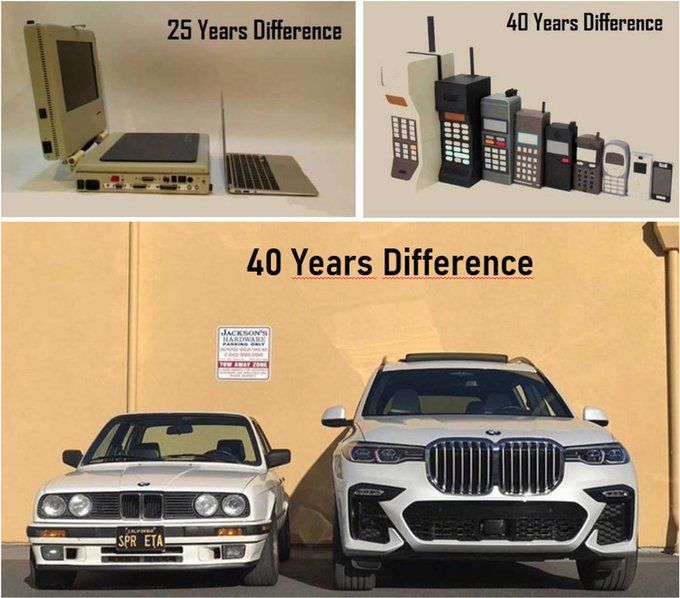
\includegraphics[keepaspectratio]{1_understanding/images/rebound-effect-fietsprofessor.jpg}}

}

\caption{\label{fig-rebound-effect-fietsprofessor}Rebound effect
illustrated using the example of the automotive industry. Source:
\href{https://www.linkedin.com/posts/brommelstroet_any-intelligent-fool-can-make-things-bigger-activity-7093961897523204096-J7A4?utm_source=share&utm_medium=member_desktop&rcm=ACoAAES-3CUB7iVY2K4QzAF6kE22k9i-b_9D8T0}{@fietsprofessor}
on LinkedIn.}

\end{figure}%

\end{minipage}%
%
\begin{minipage}{0.50\linewidth}

\begin{quote}
``Any intelligent fool can make things bigger, more complex, and more
violent. It takes a touch of genius --- and a lot of courage to move in
the opposite direction.'' E.F. Schumacher (1973)
\end{quote}

\end{minipage}%

\end{figure}%

Critics of the efficiency principle warn of the rebound effect, also
known as the Jevons paradox (Jevons 1865/1965) . This phenomenon occurs
when efficiency improvements lead to lower prices for goods and
services, thus increasing demand and negating the initial benefits of
lower resource use.

Take this simple example: If passenger cars become cheaper due to
improvements in efficiency, then people may choose a larger model when
they next purchase a car. In addition, a fuel-efficient car is cheaper
to run, as it requires less fuel per kilometre. This usually
incentivizes people to drive more (either by making more frequent
journeys or travelling longer distances) and reduce their use of public
transport or their bicycle. As a result, efficiency gains that are
technically possible are often not realized in practice, as the product
in question is used more frequently or more intensively. Apart from the
direct change in the use of the product (direct rebound), there may be
additional changes in consumer behaviour that affect the environment. In
this example, this could mean that the money saved on purchasing or
using the car is spent on air travel instead (indirect rebound), which
in turn cancels out some of the environmental benefits.

\begin{figure}[H]

\centering{

\pandocbounded{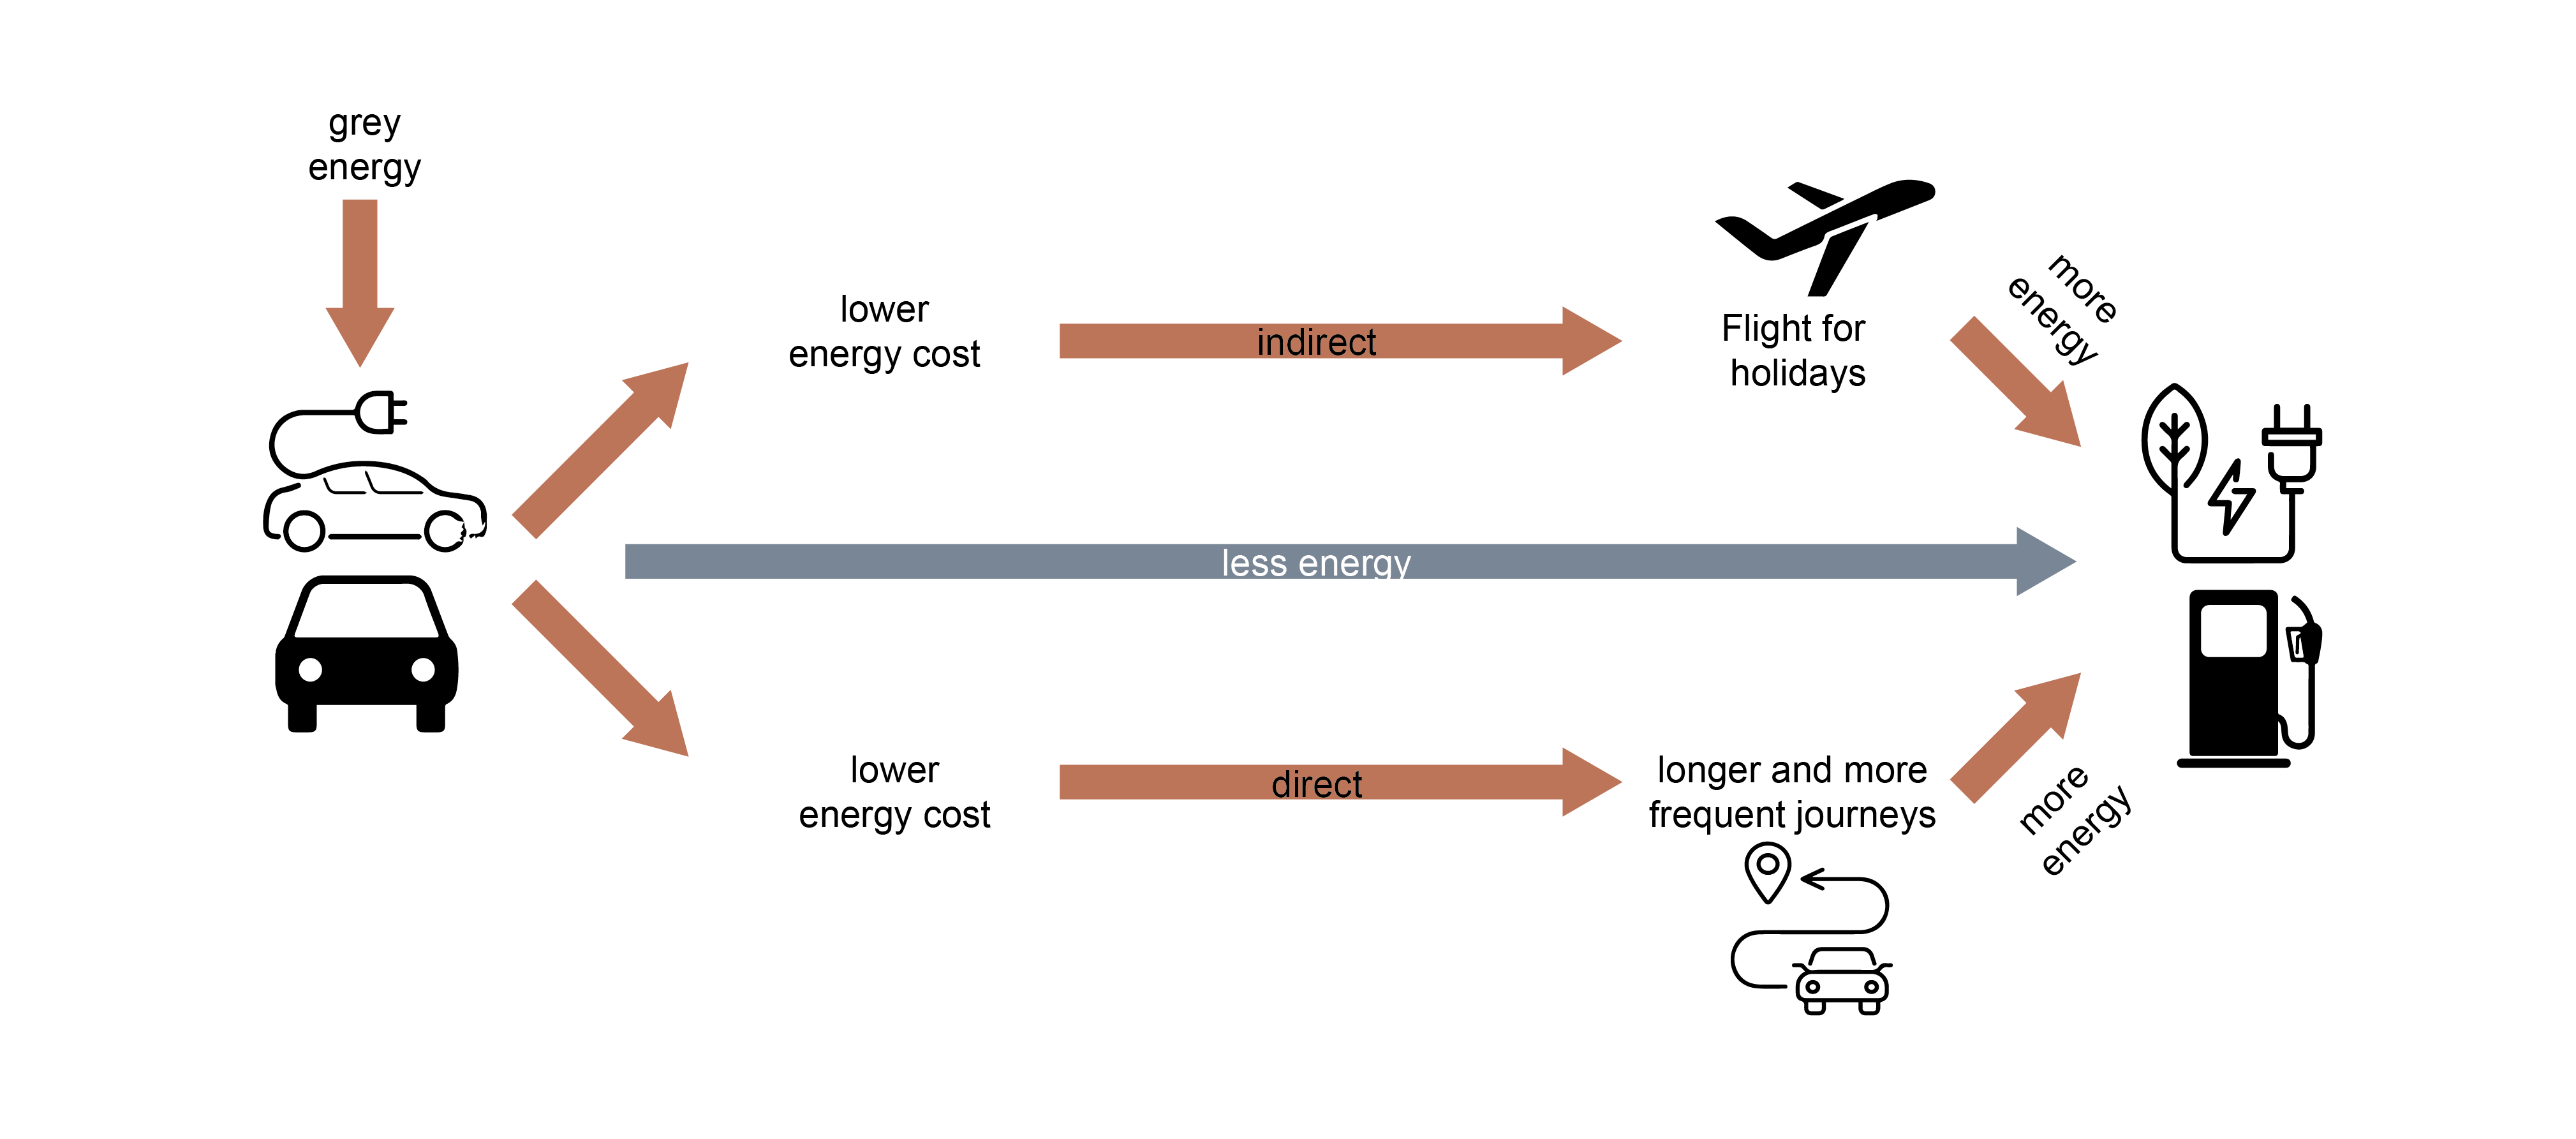
\includegraphics[keepaspectratio]{1_understanding/images/rebound-effect.png}}

}

\caption{\label{fig-rebound-effect}Indirect and direct rebound effects
of energy-saving passenger cars (Own illustration).}

\end{figure}%

To understand the rebound effect, the literature focuses on the
following three areas: 1) financial factors, 2) socio-psychological
influences, and 3) regulatory effects, which we analyse in more detail
below.

\begin{enumerate}
\def\labelenumi{\arabic{enumi}.}
\tightlist
\item
  Financial factors are a major cause of the rebound effect. When
  efficiency leads to cost savings, financial resources are freed up.
  This can lead to people either consuming more of the same product
  (direct rebound effect) or investing in alternative goods (indirect
  rebound effect). The financial rebound effect can be based on several
  factors, including:

  \begin{itemize}
  \item
    The income effect: when efficiency leads to real income gains for
    consumers, it can result in a direct or indirect rebound effect.
  \item
    The reinvestment effect: when companies use cost savings to expand
    their production or invest in other products.
  \item
    The market price effect: the macroeconomic effect in which demand in
    one sector stimulates demand in other sectors. For example, as cars
    become more efficient, demand for fuel may fall, making fuel cheaper
    and affecting demand in other energy-consuming sectors.
  \end{itemize}
\end{enumerate}

The extent and intensity of the financial rebound effect depends on
factors such as price elasticity and consumer behaviour. While this
happens at the individual level, it can cumulate into a macroeconomic
market price effect with far-reaching consequences.

\begin{enumerate}
\def\labelenumi{\arabic{enumi}.}
\setcounter{enumi}{1}
\item
  Socio-psychological influences include the ``mental accounting'' of
  individual consumers. For example, consumers who have purchased an
  efficient product may ``allow themselves'' to consume more. This is
  why increases in the efficiency of products that were previously
  considered harmful to the environment can, paradoxically, lead to an
  increase in consumption. This direct rebound effect is often referred
  to in social psychology as the ``moral hazard effect''. If the
  decision to increase consumption is not made rationally, this is known
  as the ``moral leaking effect''. For example, if you drive more after
  buying a resource-efficient car, because the purchase alone is
  perceived as environmentally conscious. The indirect rebound effect
  can also be attributed to socio-psychological factors. The ``moral
  licensing effect'' states that the purchase of resource-efficient
  products can lead to an increase in the consumption of other products
  that may be harmful to the environment. For example, when the purchase
  of a fuel-efficient car is used to justify more frequent air travel.
\item
  Sometimes, government regulations or incentives to promote efficient
  technologies can have unintended consequences -- this is what we mean
  by the ``regulatory effect''. For example, if people are encouraged to
  purchase large electrical appliances devices due to government
  incentives for energy-efficient models. Such incentives may result in
  more frequent purchases of appliances, which -- even if the newer
  model is more efficient than the old -- partially cancels out the
  energy-savings effect. Furthermore, the introduction of efficiency
  technologies leads to new capacities and infrastructures, which can
  result in the creation of new markets. Wind turbines, for example,
  promote the development of new infrastructures and jobs, but at the
  same time require considerable resources. In addition, consumers who
  purchase a more efficient product may not necessarily discard their
  old product. Some end up using both products, which can lead to
  increased overall consumption (Santarius, 2012 ).
\end{enumerate}

\begin{tcolorbox}[enhanced jigsaw, left=2mm, arc=.35mm, titlerule=0mm, opacityback=0, leftrule=.75mm, title={Rebound-effects}, breakable, bottomtitle=1mm, rightrule=.15mm, coltitle=black, toptitle=1mm, bottomrule=.15mm, colback=white, opacitybacktitle=0.6, colbacktitle=quarto-callout-note-color!10!white, toprule=.15mm, colframe=quarto-callout-note-color-frame]

The \textbf{direct rebound effect} occurs when improved energy
efficiency makes it cheaper to consume a resource, leading people to
consume more of it. For example, a more fuel-efficient car would be
cheaper to run. This might encourage people to drive more, partially or
completely cancelling out the energy savings from the efficiency
increase.

The \textbf{indirect rebound effect} occurs when energy savings or
resource efficiency gains in one area lead to the use of the freed-up
resource in other area. This reduces the overall savings achieved. For
example, if the money saved from more energy-efficient living is used
instead for more frequent flying.

\end{tcolorbox}

\subsection{How big is the rebound
effect?}\label{how-big-is-the-rebound-effect}

It is difficult to know exactly how big the rebound effect is: empirical
estimates vary widely, depending on the methods used and the effects
taken into account. It is particularly challenging to clearly
distinguish rebound effects from growth or structural changes. The type
of products and services offered also influences the level of the
rebound effect. For example: If a more economical means of transport is
used for the daily commute, such as a more efficient car, costs fall,
but the available time remains limited. Therefore, you cannot commute as
often or for as long as you like, because there are only 24 hours in a
day. The rebound effect is therefore relatively small in this case. The
situation is different for leisure activities, such as travelling by
air. If costs fall due to more efficient aircraft or cheaper prices,
there is a greater incentive to fly more often --- for example, taking a
second weekend trip instead of just one per year. As time is not such a
tight constraint here, additional consumption can increase significantly
--- as can the rebound effect. Another important component is the degree
of saturation with goods and services. Observations show that rebound
effects tend to be lower in high-income countries than in developing
countries, where there is still a considerable need for additional
consumption.

For example, the direct rebound effects associated with improvements in
space heating efficiency might lead to 10-30\% less energy savings than
what's technically possible (e.g.~Hediger et al., 2018). The rebound
effects of transport vary even more. According to Anderson et
al.~(2019), the rebound effect related to private mobility might reduce
potential savings by 7.5\% in Denmark, 30\% in Sweden, and 60\% in
Germany. In contrast, studies on lighting in private households have
found very low rebound effects of less than 10\% (Sorrell, 2007). This
means that the actual energy savings for these services can be, on
average, up to 25\% less than what is technically possible and
predicted. However, the exact magnitude of the rebound depends on the
specific context and can be reduced by choosing appropriate measures.

Sometimes, albeit rarely, the savings may be overcompensated. This is
known as the ``backfire'' effect. However, this is an exception and the
``backfire'' effect is not a pure rebound effect, as it is linked to the
effects of growth and structural change. A good example is
digitalization, which can lead to short- and medium-term backfire
effects (Peng et al., 2023).

\part{Approaches to Sustainability}

\chapter{Approaches to
Sustainability}\label{approaches-to-sustainability-1}

\section{Approaches to Sustainable
Development}\label{approaches-to-sustainable-development}

\emph{Christoph Bader}

The world is facing numerous challenges of sustainable development,
including pressing environmental problems and social inequalities.
Scientists, researchers, and activists are seeking innovative approaches
to enable sustainable and equitable change. This chapter examines some
of these approaches, which offer a complete rethink of current
paradigms. Approaches discussed in this chapter:

\begin{itemize}
\item
  Planetary boundaries framework
\item
  Doughnut economics
\item
  Approaches to a ``great transformation''
\item
  Green economy
\item
  Post-growth approaches
\item
  Implementing the 2030 Agenda
\end{itemize}

\section{Debates about planetary
boundaries}\label{debates-about-planetary-boundaries}

In 1798, British economist Thomas Robert Malthus published his
influential essay, \emph{An Essay on the Principle of Population}.
Malthus's core idea was that population growth would surpass Earth's
ability to produce food, sparking a debate on planetary carrying
capacity that continues today. \emph{The Limits to Growth} (1972), a
report by the Club of Rome, built on Malthus's ideas. It went beyond
just food supply to consider a broader range of factors in calculating a
planetary limit. These factors included resource availability,
environmental pollution, and industrial output. The report remains
relevant from an environmental point of view, as it challenges the
assumptions of limitless growth, even though its specific predictions
haven't quite come true.

A significant development in sustainability science is the planetary
boundaries concept, introduced in 2009. Unlike earlier theories focused
solely on population limits, this framework uses Earth system science
parameters. Researchers identified the Holocene epoch as a baseline, as
this was a period of remarkable stability for human development.
Significant deviations from this ideal state could push humanity towards
uncertain ``tipping points'' -- critical thresholds that can either
interrupt previous progress, alter its course, or even accelerate it in
unintended ways. An example might be the extinction of megafauna at the
end of the last ice age, potentially linked to human arrival in the
Americas. The planetary boundaries concept promotes the precautionary
principle, urging action to minimize potential harm to both humans and
the environment.

The concept, which puts forward nine planetary boundaries, was first
introduced by Johan Rockström et al.~(2009). It was updated by Will
Steffen et al.~(2015). A recent update by Richardson et al.~(2023) shows
that six out of nine planetary boundaries have already been
transgressed.

The planetary boundaries framework identifies nine critical Earth system
processes. These processes regulate the planet's stability and include,
for example, land system change and ocean acidification (see all
planetary boundaries here:
Figure~\ref{fig-development-planetary-boundaries}). Each boundary has an
inner circle, within which it can operate safely (``safe operating
space'') and an outer circle, which represents increased uncertainty.

The latest update to the planetary boundaries framework paints a
concerning picture. We're close to overstepping the safe operating space
for ocean acidification, and regional atmospheric aerosol loading has
already crossed its boundary. In a positive development, stratospheric
ozone levels show some signs of recovery. However, the overall situation
is alarming. The boundaries previously identified as transgressed
(climate change, biosphere integrity (genetic diversity), land system
change, and biogeochemical flows {[}N and P{]}) have all seen a
worsening of their transgression since 2015.

The study added human appropriation of net primary production as a
control variable for the functional component of biosphere integrity,
arguing that this boundary has also been exceeded. In addition, the
significant transgression of the planetary boundaries for phosphorus and
nitrogen cycles, along with genetic biodiversity, raise the risk of
fatal consequences.

Two of the nine planetary boundaries -- biosphere integrity and climate
change -- are considered ``core boundaries''. These core systems
encompass processes from many other subsystems and operate at a global
scale. Reaching tipping points in these core systems could therefore
push the entire Earth system into a new state.

\begin{figure}[H]

\centering{

\pandocbounded{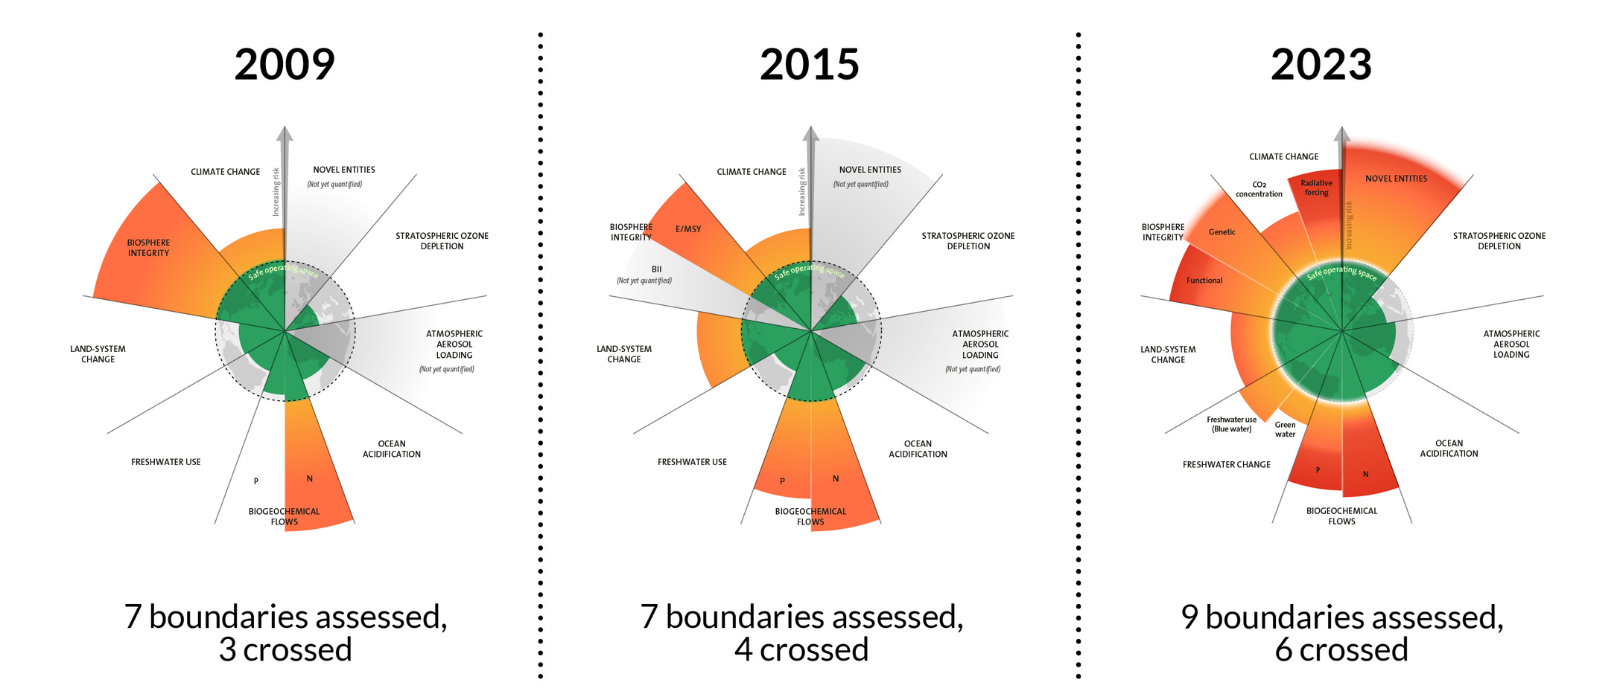
\includegraphics[keepaspectratio]{2_approaches/Images/Fig2_1__planetaryboundaries.png}}

}

\caption{\label{fig-development-planetary-boundaries}Development of
control variables for all nine planetary boundaries (Source: UNEP
(2021b))}

\end{figure}%

\subsection{Tipping points of the Earth's climate
system}\label{tipping-points-of-the-earths-climate-system}

\begin{figure}[H]

\centering{

\pandocbounded{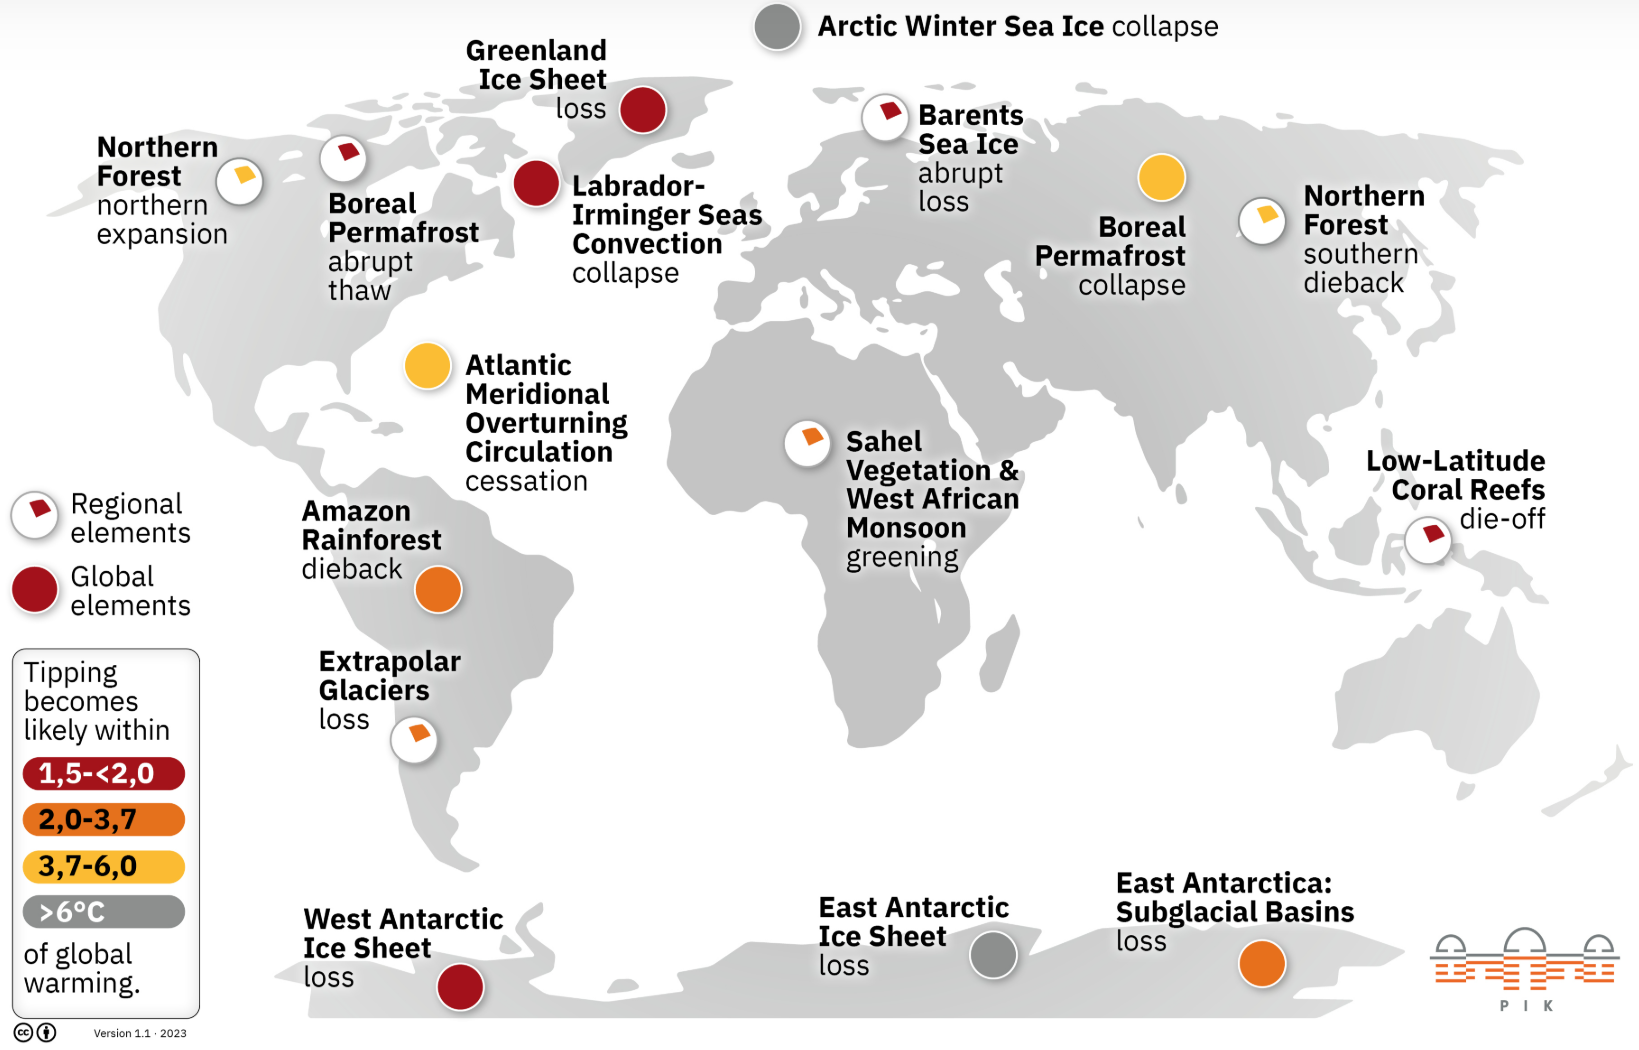
\includegraphics[keepaspectratio]{2_approaches/Images/Tippingpoints.png}}

}

\caption{\label{fig-tippingspoints}Tipping points (Source:)}

\end{figure}%

Tipping points in the Earth's climate system are critical thresholds
that, when crossed, can cause abrupt and often irreversible changes in
the climate system. These tipping points can destabilize the climate and
lead to accelerated climate change. Examples of tipping points include
the melting of the Greenland ice sheet, the collapse of the Amazon
rainforest, the thawing of permafrost soils, and changes in the Gulf
Stream. If these tipping points are reached or exceeded, they can
trigger self-reinforcing feedback effects that lead to further warming
and an intensification of climate change.

The concept of tipping points emphasizes the urgency of limiting global
warming and reducing greenhouse gas emissions. If we exceed the tipping
points, it will become increasingly difficult to control climate change
and minimize its effects.

\subsection{Quantifying planetary
boundaries}\label{quantifying-planetary-boundaries}

A recent development within the planetary boundaries framework is the
concept of ``safe and just Earth system boundaries (ESBs)'' for the
following domains: climate, the biosphere, water and nutrient cycles,
and aerosols at global and subglobal scales (Rockström et al., 2023).
The ESBs are based on modelling and literature review, and account for
uncertainty through different levels of likelihood. Staying within the
ESBs protects stability and equity between species and future
generations, although current generations, especially vulnerable groups,
could still suffer harm. The authors therefore suggest stricter
boundaries in some cases, and the addition of local standards to protect
current generations and ecosystems. For example, they identify safe ESBs
for warming (see Rockström et al.~2023, Fig. 1 and Table 1). These are
based on reducing the probability of triggering climate tipping points,
maintaining biosphere and cryosphere functions, and considering climate
variability of the Holocene (\textless0.5-1.0°C) and earlier
interglacial periods (\textless1.5-2°C).

The functions of the cryosphere include the preservation of permafrost
in the northern high latitudes, the preservation of polar ice sheets and
mountain glaciers, and the minimization of sea ice loss. The authors
conclude that global warming of more than 1.0°C above pre-industrial
levels, which has already been exceeded (IPPC 2021), could trigger
tipping effects such as the collapse of the Greenland ice sheet or a
localized abrupt thawing of the boreal permafrost with a moderate
probability (Armstrong et al.~2022). Global warming of one degree
Celsius corresponds to the safe limit proposed in 1990 and the PB of 350
ppm CO2 (Steffen et al.~2015). With a warming of more than 1.5°C or
2.0°C, the likelihood of triggering tipping points increases to high or
very high.

\subsection{Climate resilience}\label{climate-resilience}

Resilience describes the ability of a system to withstand disruptions,
``bounce back'', or recover from adversity. Originally used in
psychology, resilience refers to the psychological robustness that an
individual has actively acquired in dealing with challenges or stresses,
particularly in childhood. In the context of ecosystems, resilience
refers to the ability to absorb disturbances without a permanent
systemic collapse, i.e.~a collapse that would result in a different
system regulated by new processes (Folke et al.~2010). More recently,
the concept of resilience has been extended to social systems (see
section on doughnut economics). Studies focus on which specific
characteristics of a region need to be strengthened, to better prepare
it for future crises and disasters related to climate change, terrorism,
resource scarcity, or financial crises. The climate crisis, for example,
requires both adaptation and mitigation measures. Resilience approaches
offer a way of combining these two concepts rather than playing them off
against each other.

\textbf{Climate mitigation measures} aim to reduce greenhouse gas
emissions and curb climate change. Such measures include promoting
renewable energies, improving energy efficiency, and expanding public
transport. Resilience approaches emphasize the importance of climate
mitigation, as limiting the rise in temperature will help to reduce the
intensity and frequency of extreme weather events.

\textbf{Climate adaptation measures} aim to make societies and
ecosystems more resilient to the current and expected effects of climate
change. Adaptation measures include the development of early warning
systems for extreme weather events, coastal protection against rising
sea levels, the reduction of heat stress (e.g.~through more urban green
spaces), runoff or infiltration areas to reduce the damaging effects of
heavy rainfall events, or the adaptation of agricultural practices to
changing climatic conditions. Resilience approaches emphasize the need
for climate adaptation to protect communities and ecosystems from the
negative effects of climate change.

\subsection{Conclusion}\label{conclusion}

The concept of planetary boundaries tries to reduce complex ecological
relationships to a small number of quantifiable limits. These specific
limits and indicators for planetary boundaries are based on scientific
findings that are not always clear or consistent. The boundaries are
therefore contested by some scholars, who question the accuracy and
reliability of the data and models used. Despite this criticism, the
planetary boundaries framework makes a valuable contribution to the
debate on sustainable development and raises awareness of the limited
resources and resilience of our planet. To summarize:

\begin{itemize}
\item
  The planetary boundaries framework focuses on the
  ecological/biophysical limits of the Earth's resilience, and thus the
  environmental dimension of sustainable development.
\item
  These limits to resilience -- the planetary boundaries -- focus on
  environmental factors that are considered fundamental to human
  survival.
\item
  In normative terms, the framework aims to maintain the stable Earth
  system (``state of equilibrium'') of the Holocene, thereby mitigating
  threats to human survival.
\item
  The planetary boundaries framework can be used to set concrete targets
  in the environmental dimension (e.g.~at the global or national level).
\end{itemize}

Further readings

Lenton TM, Rockström J, Gaffney O, Rahmstorf S, Richardson K, Steffen W,
Schellnhuber HJ. 2019. Climate tipping points --- too risky to bet
against. \emph{Nature}. 575(7784):592--595.
doi:\href{https://doi.org/10.1038/d41586-019-03595-0}{10.1038/d41586-019-03595-0}.

Rockström J, Gupta J, Qin D, Lade SJ, Abrams JF, Andersen LS, Armstrong
McKay DI, Bai X, Bala G, Bunn SE, et al.~2023. Safe and just Earth
system boundaries. \emph{Nature}. 619(7968):102--111.
doi:\href{https://doi.org/10.1038/s41586-023-06083-8}{10.1038/s41586-023-06083-8}.

Folke C, Carpenter SR, Walker B, Scheffer M, Chapin T, Rockström J.
2010. Resilience Thinking: Integrating Resilience, Adaptability and
Transformability. \emph{Ecology and Society}. 15(4)..
\url{https://www.jstor.org/stable/26268226}.

\section{From planetary boundaries to the doughnut
model}\label{from-planetary-boundaries-to-the-doughnut-model}

Economist Kate Raworth's Doughnut Model is an innovative approach to
sustainable development that recognizes social and environmental limits.
This requires rejecting much of what has characterized
20\textsuperscript{th}-century economics, as Raworth outlines in her
2017 book, \emph{Doughnut Economics: Seven Ways to Think Like a 21st
Century Economist}. Raworth depicts the ideal economy of the future in a
simple image: a ring-shaped doughnut. The outer ring symbolizes an
ecological ceiling that should not be crossed, as doing so would cause
irreversible harm to the environment. The inner ring represents a social
foundation covering people's basic needs, such as food, housing, and
income. The challenge is to ensure that economic activities take place
within this ring -- the doughnut -- to ensure the well-being of both
humanity and the environment (``safe and just space for humanity'').

\begin{figure}[H]

\centering{

\pandocbounded{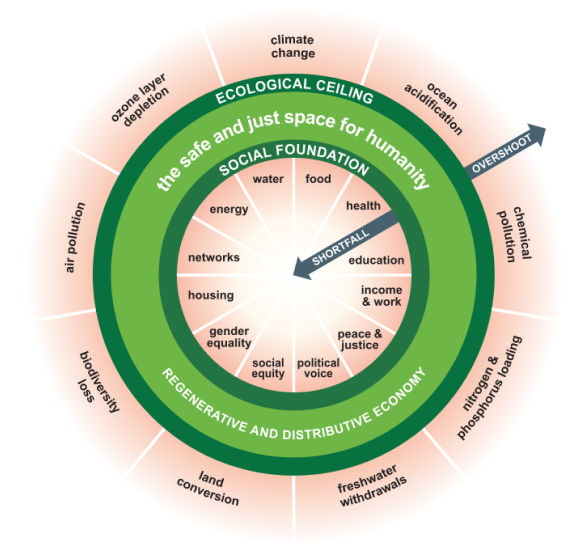
\includegraphics[keepaspectratio]{2_approaches/Images/Fig2_3__doughnut.png}}

}

\caption{\label{fig-doughnut}Doughnut Model
(Source:https://doughnuteconomics.org)}

\end{figure}%

The philosophy of the doughnut approach is based on three core
principles: equitable distribution of wealth, regeneration of the
resources used by the economy, and creation of wealth for all people.
None of these principles should have to depend on economic growth, says
Raworth. In other words, we don't need to pursue unlimited growth for
the economy to flourish -- instead, we should pursue development that is
sustainable, balanced, and equitable. The transition to the doughnut
model requires a fundamental change in the way we think and act. It's
about moving from a growth paradigm to sustainable development, a
development that takes social justice and environmental sustainability
into equal account.

\subsection{Conclusion}\label{conclusion-1}

Despite the Doughnut Model's focus on the economy, critics say it
doesn't discuss the underlying framework conditions (i.e.~the
structures, rules, and institutional organization of the economy) or how
money is created and managed (i.e.~the financial sector). The Doughnut
Model focuses on what kind of economic activity is desirable
(i.e.~staying within the doughnut), but it doesn't explain how to get
there. These points of criticism are being addressed by the Doughnut
Economics Action Lab (DEAL), which provides tools and strategies to
implement the Doughnut Model in real-world settings.

\begin{itemize}
\item
  The Doughnut model builds on the concept of planetary boundaries,
  adding a social dimension and including goals and degrees of goal
  achievement.
\item
  In normative terms, the model prescribes that

  \begin{itemize}
  \item
    social goals should be achieved without overstepping the planetary
    boundaries. The planetary boundaries provide the biophysical
    framework within which the social goals should be achieved.
  \item
    when setting concrete goals, measures etc. at sub-global levels, the
    global social goals must also be taken into account.
  \end{itemize}
\end{itemize}

\section{The debate about the Great
Transformation}\label{the-debate-about-the-great-transformation}

Concepts of the ``great transformation'' refer to fundamental changes in
social, economic, political, and ecological systems that are necessary
to create a sustainable and just society.

``Great transformation'' was a term used by Karl Polanyi in his 1944
analysis that the shift to a free market in the 19th century brought
about profound social, economic, and political changes that
fundamentally transformed people's lives and relationship with nature.
Polanyi argued that unbridled market dynamics caused social and
environmental problems, and that society needed to develop mechanisms to
regulate and balance these problems. Similarly, today's concepts of the
great transformation emphasize the importance of regulation,
redistribution, and the development of alternative economic models to
create a sustainable and just society. While Polanyi stressed the need
for social protection measures and the importance of integrating markets
into social structures, current concepts of the great transformation
additionally aim to fundamentally change production and consumption
patterns to reduce environmental impact.

\subsection{\texorpdfstring{Flagship WBGU report: \emph{World in
Transition}}{Flagship WBGU report: World in Transition}}\label{flagship-wbgu-report-world-in-transition}

A flagship report by the German Advisory Council on Global Change
(WBGU), \emph{World in Transition,} is an important publication that
addresses the challenges and opportunities of a sustainable
transformation of society. It was first published in 1994 and has since
been updated several times. The report analyses global environmental
changes, including climate change, biodiversity loss, and resource
consumption, and proposes concrete policies and social change to promote
sustainable development.

\emph{World in Transition} is significant to debates on the great
transformation, as it argues for a far-reaching transformation of
business, policy, and society. This vision extends beyond mere
adaptation, demanding fundamental shifts in the structures and patterns
of economic activity and daily life. The report underscores the urgency
of driving forward the transition to a climate-friendly and
environmentally sound economy and way of living. It emphasizes the
critical role of a comprehensive sustainability policy. Finally, it
identifies innovation, technology, education, institutional reforms, and
international cooperation as key levers for achieving sustainable
development.

\begin{figure}[H]

\centering{

\pandocbounded{\includegraphics[keepaspectratio]{2_approaches/Images/.png}}

}

\caption{\label{fig-new-social-contract}New social contract (Source:
WBGU 2011, p.~275)}

\end{figure}%

In Chapter 8, \emph{World in Transition} distinguishes between two
concepts: ``transformation research and education'' and ``transformative
research and education''. These concepts are key to promoting
fundamental change towards sustainability.

\emph{Transformation research} analyses processes of change,
particularly in the context of sustainable development. It seeks to
understand the dynamics and complexity of transformations, and to
identify possible courses of action for a sustainable future.
Transformation research offers an inter- and transdisciplinary
perspective, and it involves different actors and stakeholders in the
research process.

\emph{Transformation education} is education that aims to impart the
knowledge, skills, and values needed to achieve a sustainable
transformation of society. It includes formal and informal educational
measures that enable people to actively participate in transformation
processes and to promote sustainable thinking and action.

\emph{Transformative research} not only generates knowledge but also
goes a step further, by actively striving for change towards
sustainability. It thus aims to influence social practice and develop
solutions and innovations for sustainable development. Transformative
research works closely with partners from practice, and strives to
translate knowledge into action.

\emph{Transformative education} fosters a shift in mindsets, values, and
behaviour towards sustainability. It goes beyond imparting knowledge, by
also promoting critical awareness, empathy, and action for sustainable
changes in society.

The WBGU believes that the state should take on tasks that are not
adequately performed by individuals or the private sector. It recognizes
that the state plays a decisive role in creating framework conditions
and shaping political measures to promote sustainable development. The
state can drive innovative solutions, steer investments, establish
regulations, and implement policies that enable a sustainable
transformation.

\begin{quote}
``The important thing for Government is not to do things which
individuals are doing already, and to do them a little bit better or a
little worse; but to do those things which at present are not done at
all.''

--- John M. Keynes, The End of Laissez-Faire, 1926
\end{quote}

However, the WBGU also emphasizes that effective government intervention
should take place in collaboration with other actors and stakeholders,
including civil society, the private sector, and academia. Jointly
shaping a sustainable future is about creating partnerships and
involving different expertise.

\subsection{Schneidewind's ``art of the
future''}\label{schneidewinds-art-of-the-future}

The German economist and politician, Uwe Schneidewind, discusses the
concept of the great transformation in his 2018 book, \emph{Die grosse
Transformation: Eine Einführung in die Kunst des gesellschaftlichen
Wandels}, which translates as \emph{The Great Transformation: An
Introduction to the Art of Social Change}. Schneidewind points out that
a great transformation isn't dictated by the unstoppable development
dynamics of modern societies or by a technocratic blueprint for an
ecologically just society. Instead, he sees it as a process that should
be actively shaped by many actors. As such, it's important to have a
clearly defined normative compass and to develop the ability to navigate
complex social, cultural, economic, and technological processes. He
describes this ability as the ``art of the future'' -- the skill of
making desirable futures possible -- and thus builds a bridge to Harald
Welzer's FUTURZWEI. Welzer, a psychologist and sociologist, emphasizes
the importance of imagination, creativity, and engagement in bringing
about transformative change and developing alternative visions of the
future.

\begin{figure}[H]

\centering{

\pandocbounded{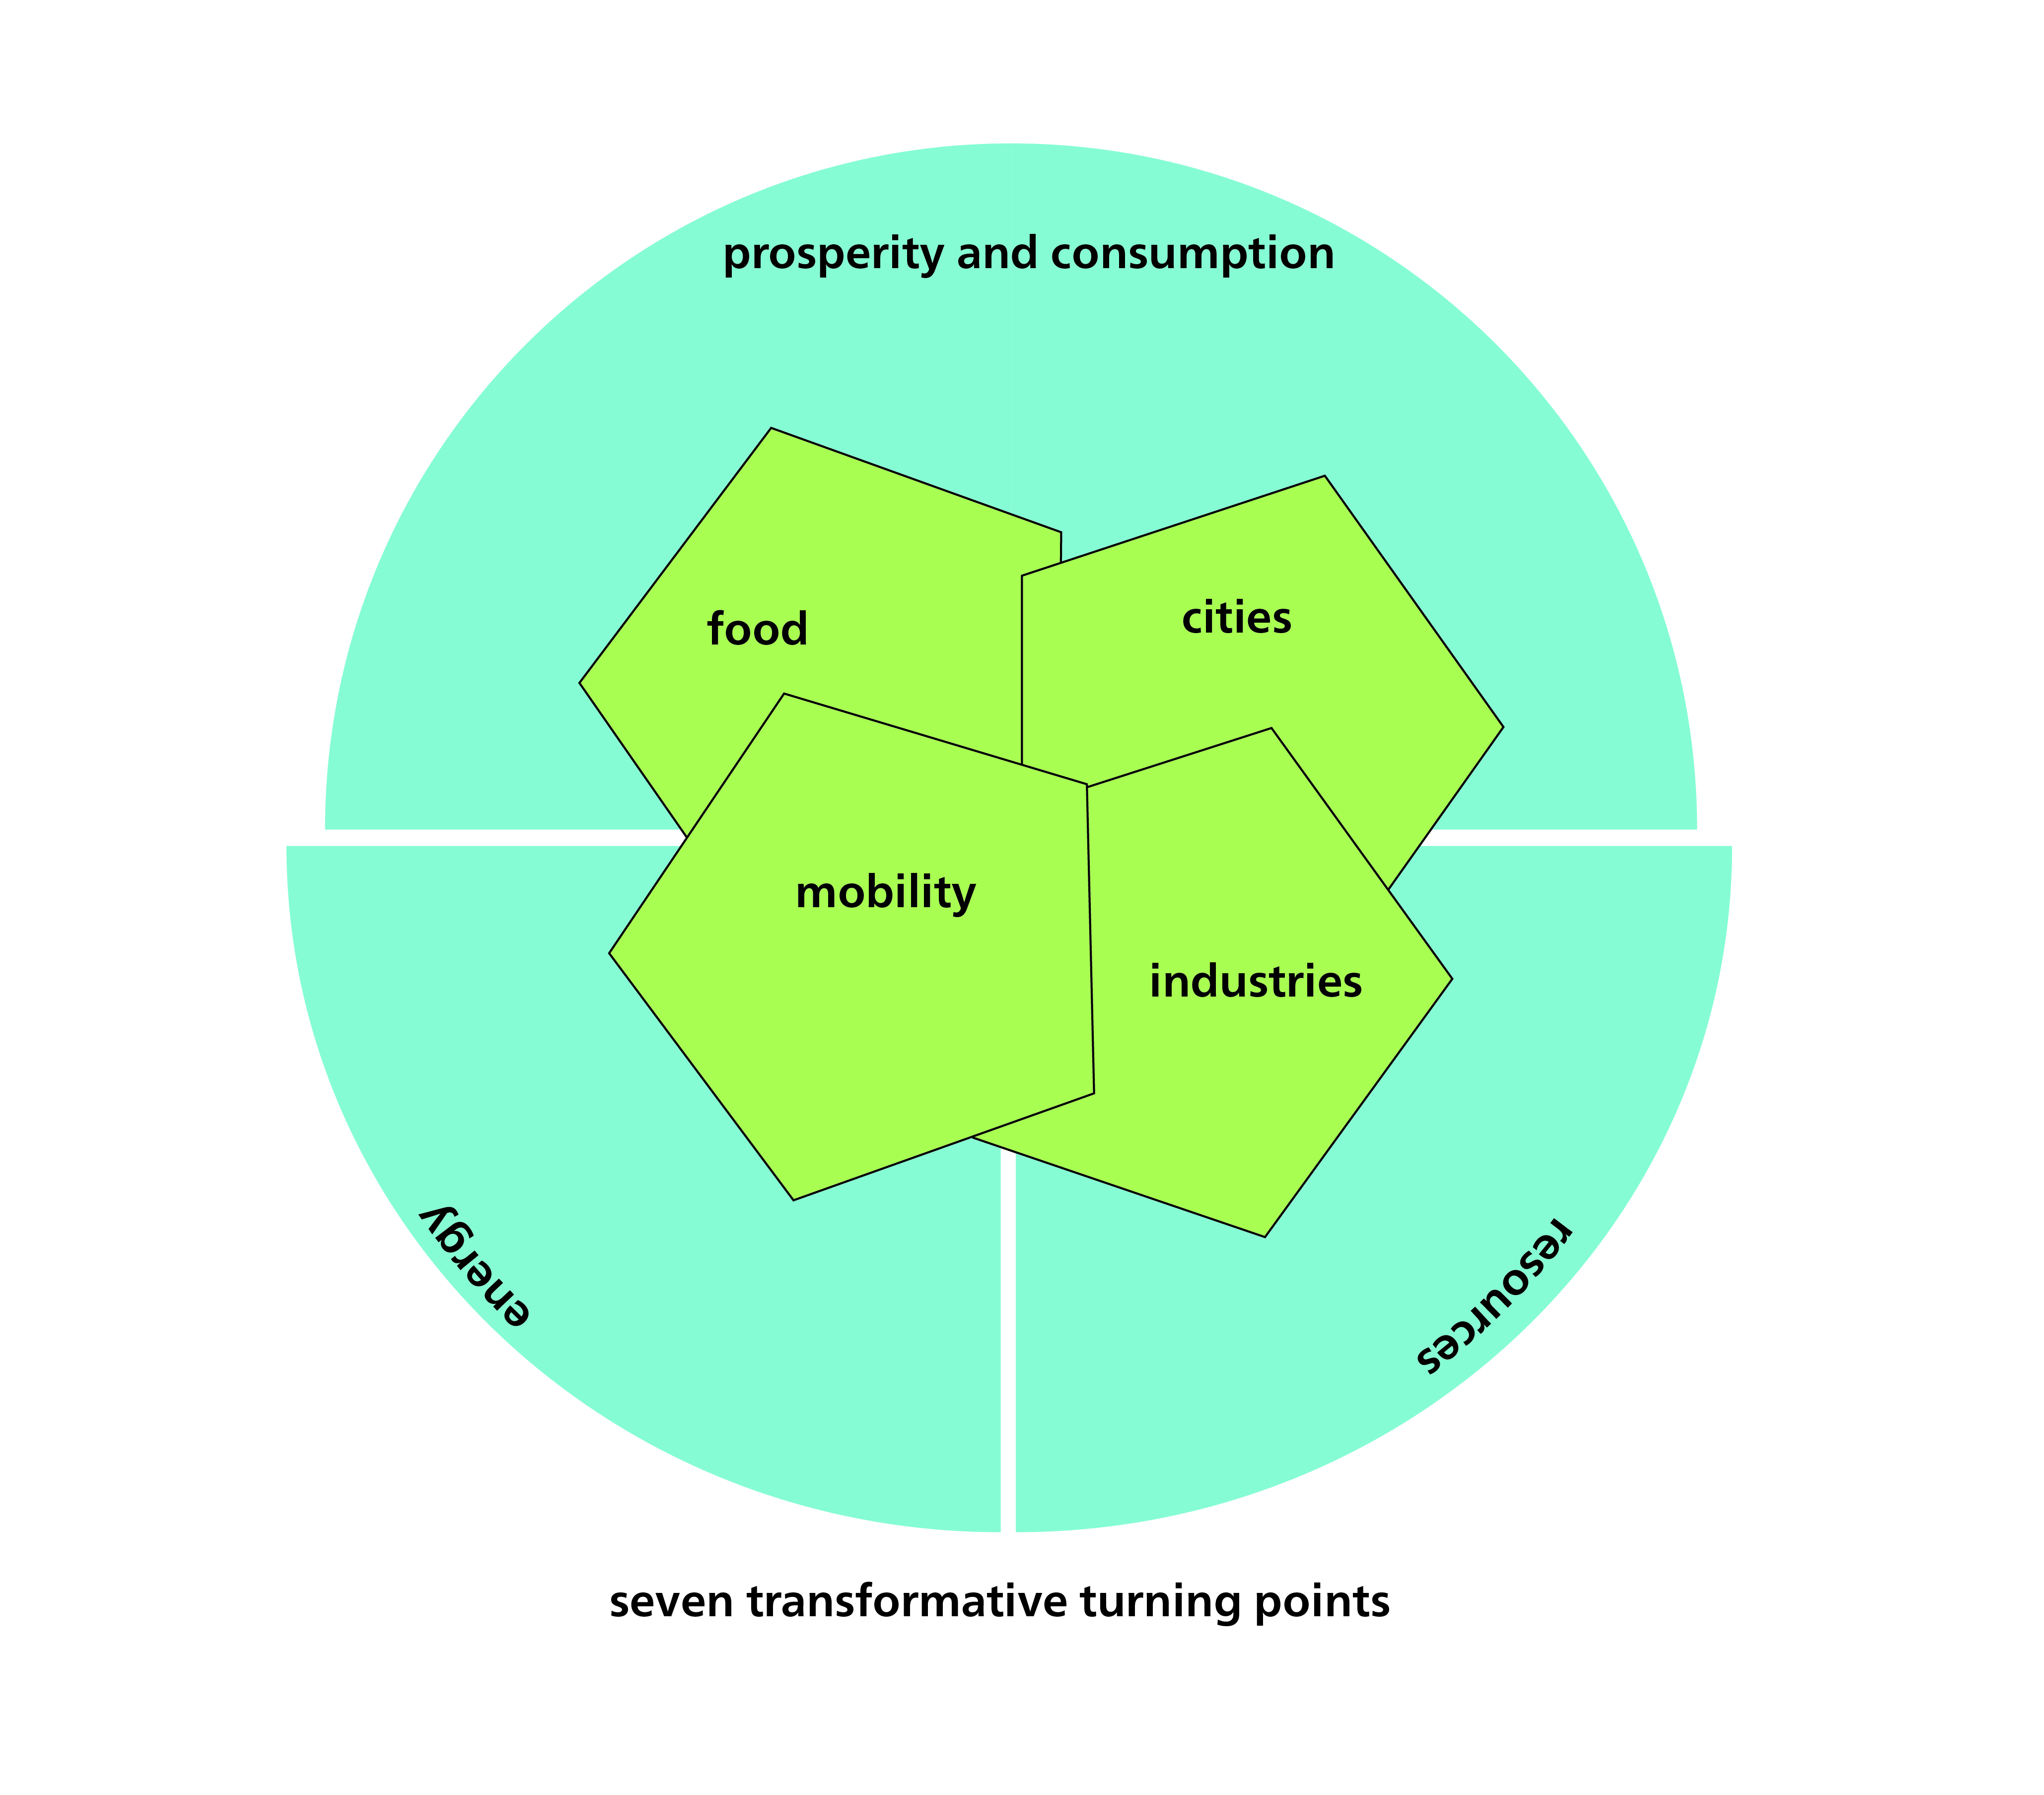
\includegraphics[keepaspectratio]{2_approaches/Images/Fig2_5_Schneidewind_turningpoints.jpg}}

}

\caption{\label{fig-turningpoints}Schneidewinds turningpoints (Source:
Schneidewind (2018))}

\end{figure}%

For Schneidewind, the great transformation has seven transformative
turning points. The four dimensions of the ``art of the future''
(technological, economic, cultural, institutional) can be found in all
seven turning points. Resource and energy transformations are
fundamental. However, according to the concept of ``double decoupling'',
they are inconceivable without a comprehensive transformation in ideas
surrounding prosperity and consumption. Envisaging the desired
transformation is easier in more specific sectors, such as mobility,
food, cities, and key energy- and resource-intensive industries.

\begin{figure}[H]

\centering{

\pandocbounded{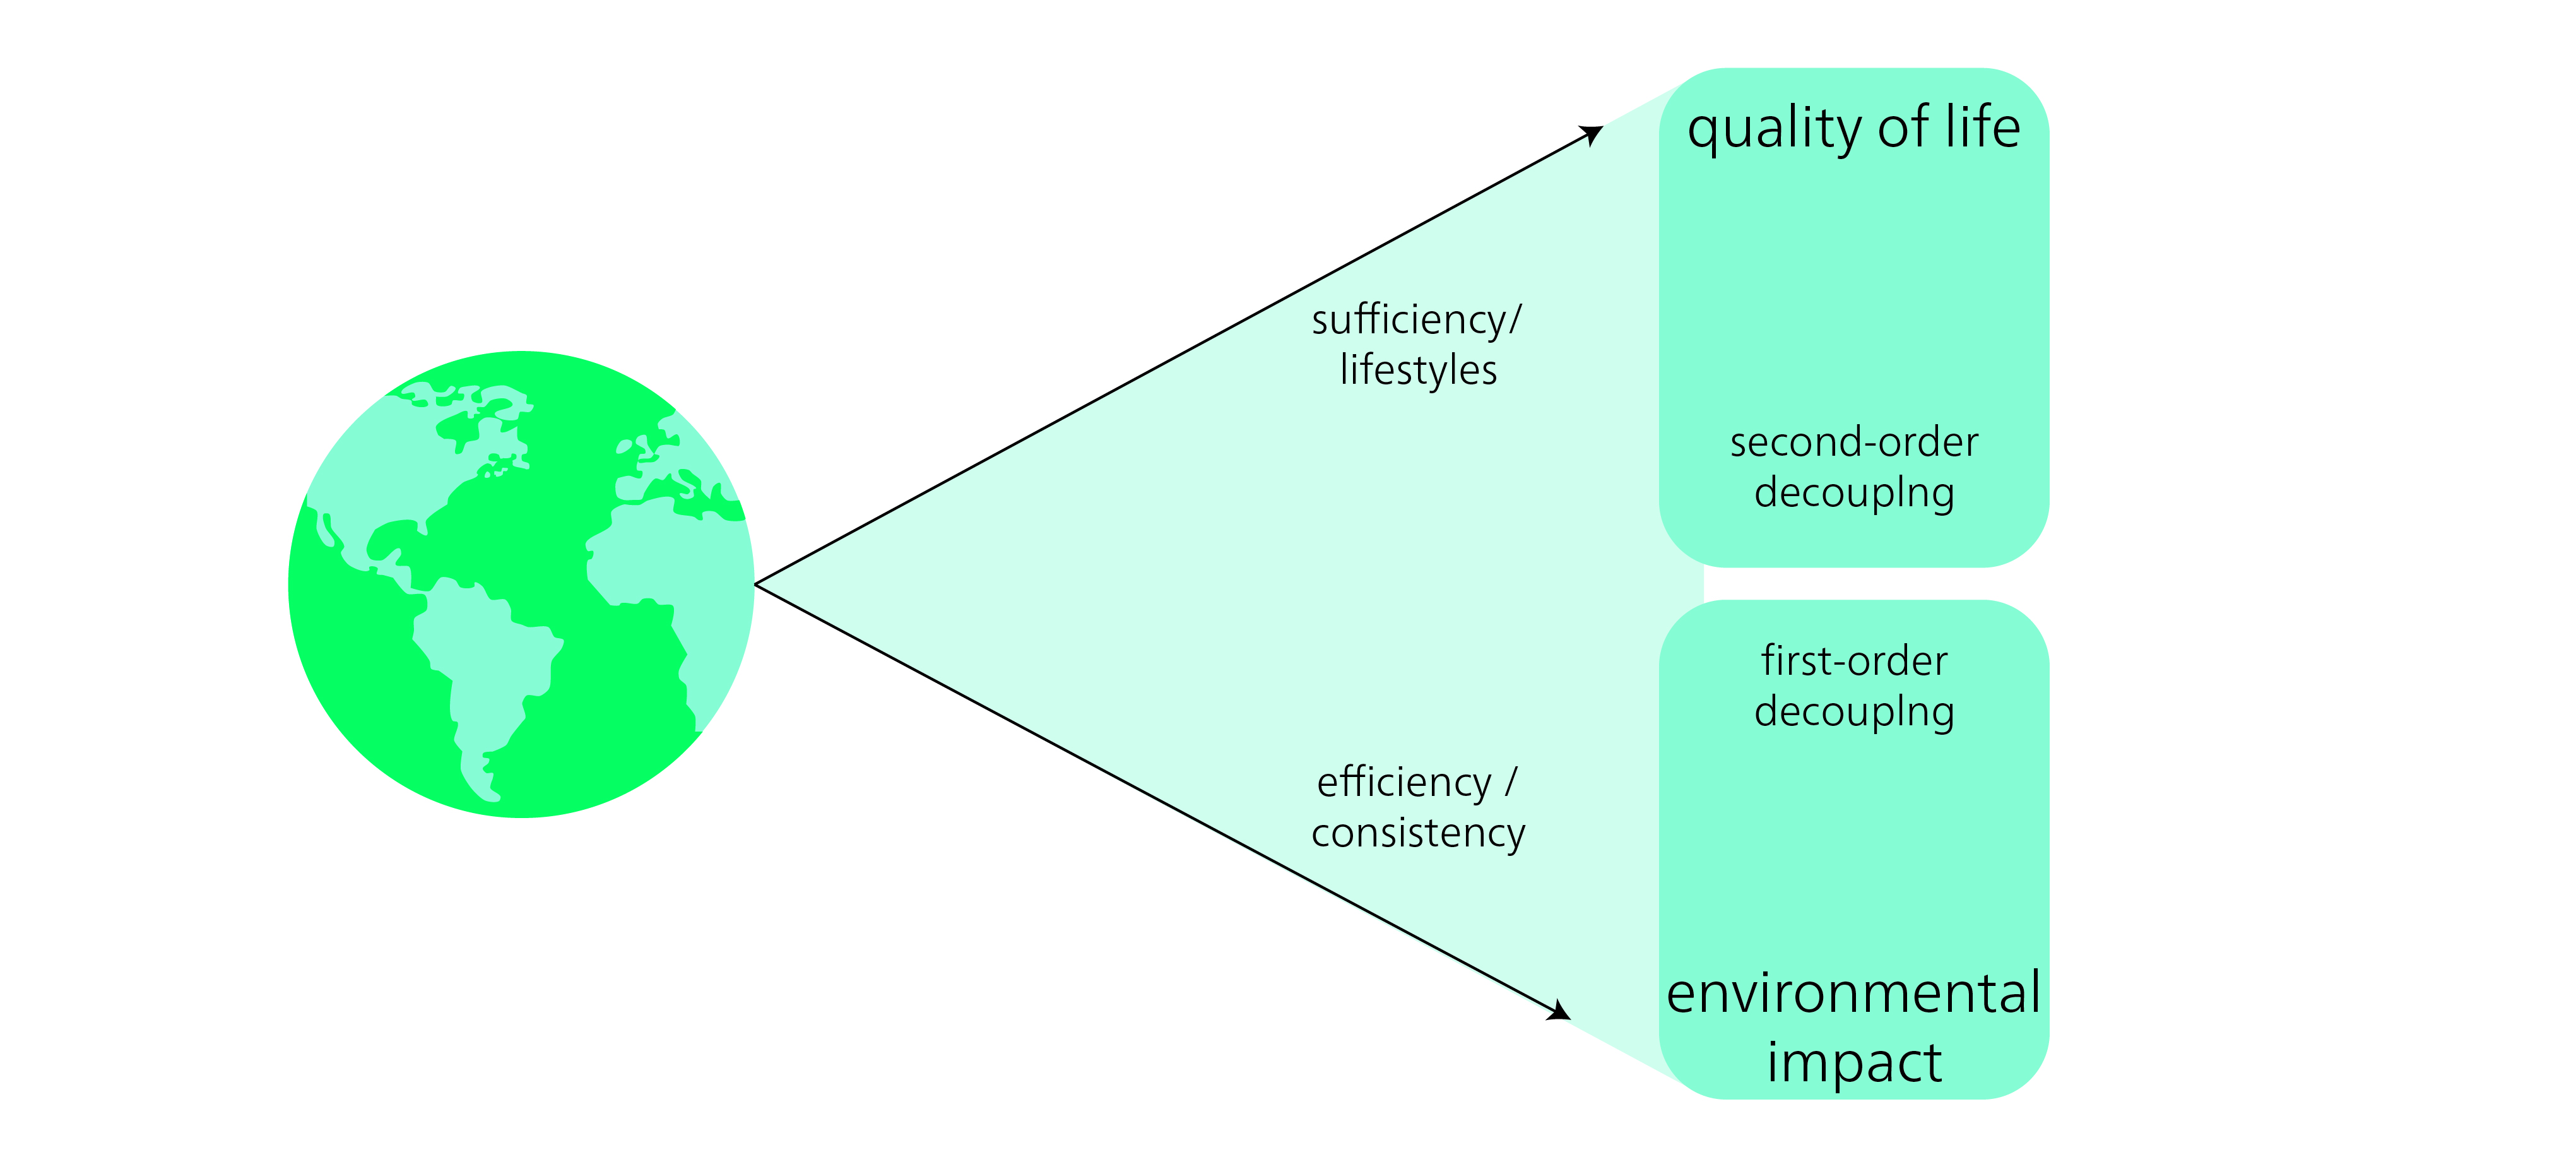
\includegraphics[keepaspectratio]{2_approaches/Images/Fig2_6__double_decoupling.jpg}}

}

\caption{\label{fig-double-decoupling}Double decoupling (Source:
Schneidewind (2018))}

\end{figure}%

``Decoupling'' refers to the separation of economic activity from
environmental impact. A key concept in the sustainability debate,
\textbf{double decoupling} states that sustainable development can only
be achieved through increases in technological efficiency in combination
with new models of prosperity and consumption. It aims to promote a more
comprehensive and systemic understanding of innovation, to include both
technological and social innovations.

Double decoupling refers to the following two types of decoupling:

\begin{itemize}
\item
  First-order decoupling: This focuses on increasing resource efficiency
  and consistency within the traditional economic growth model, mainly
  through technological advancements, and
\item
  Second-order decoupling: This focuses on ``sufficiency'', decoupling
  quality of life and a ``good life'' from the traditional economic
  growth model, as measured by GDP.
\end{itemize}

\subsection{Global Sustainable Development
Report}\label{global-sustainable-development-report}

In September 2019, the first Global Sustainable Development Report
(GSDR) was published by a group of 15 independent scientists appointed
by the UN Secretary-General. Intended for publication every four years,
the aim of the GSDR is to synthesize existing knowledge and identify
pathways to achieving the Sustainable Development Goals (SDGs). The
latest report (2023) highlights the significant gap between current
progress and achieving the SDGs. Building on the 2019 report, it
introduces capacity building as a new lever to accelerate progress.

\begin{figure}[H]

\centering{

\pandocbounded{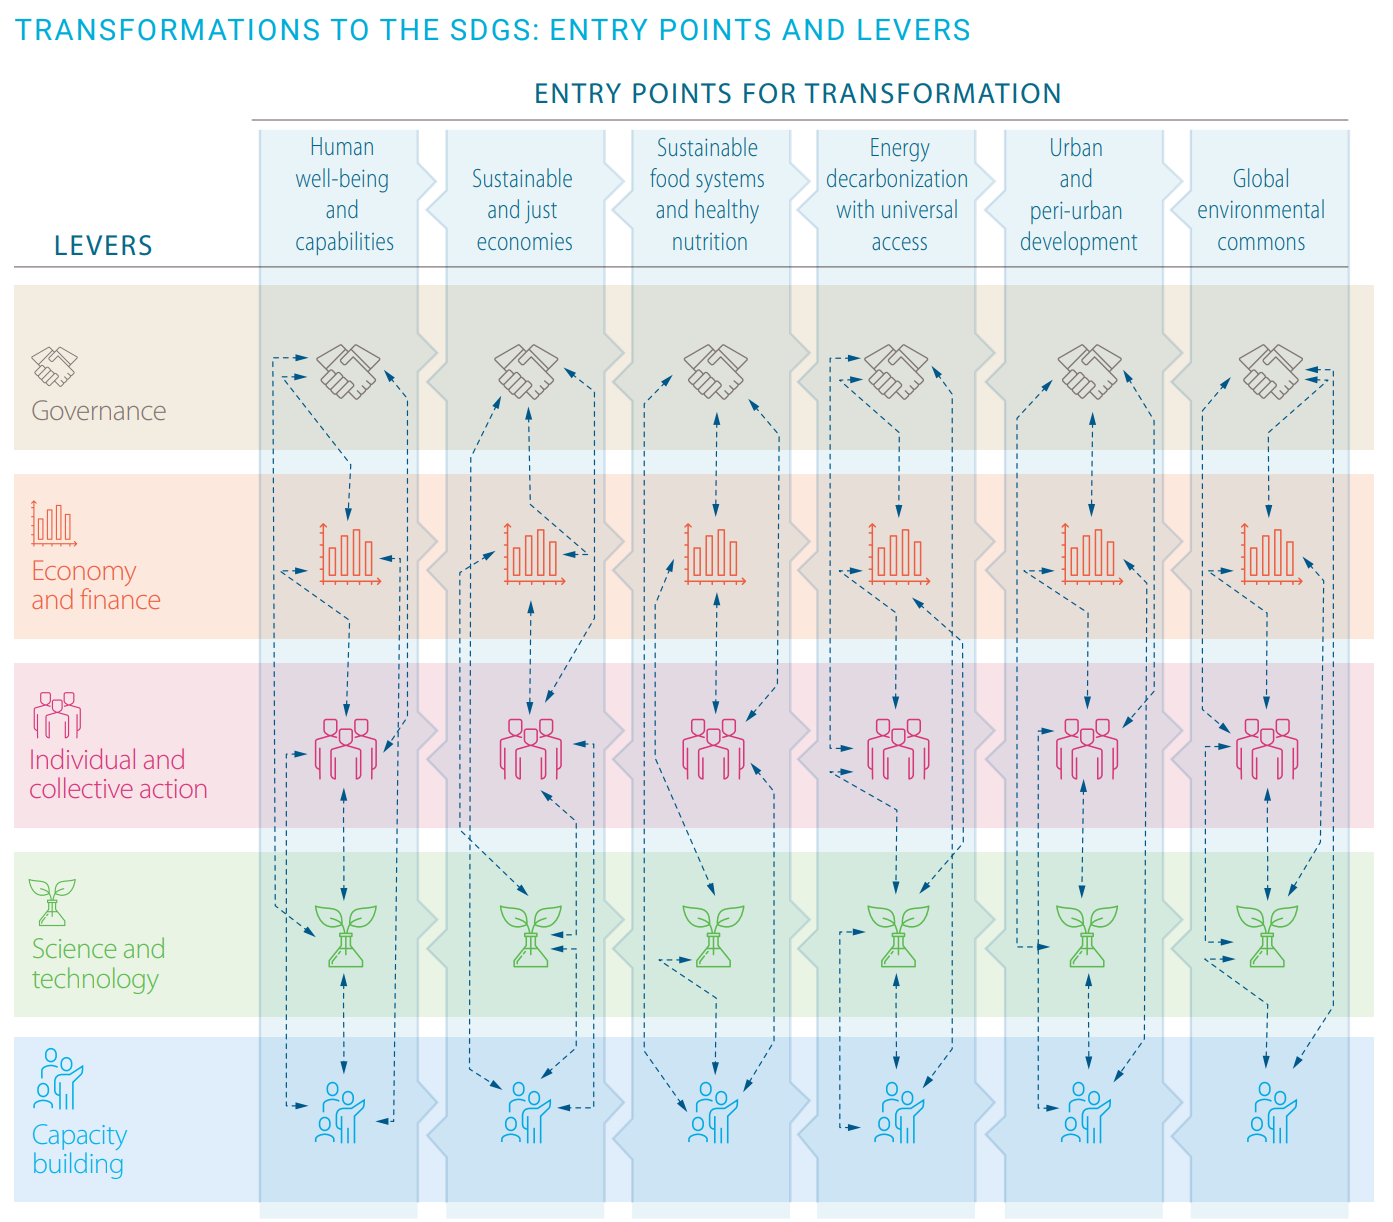
\includegraphics[keepaspectratio]{2_approaches/Images/Fig2_7__GSDR.png}}

}

\caption{\label{fig-GSDR}GSDR (Source: GSDR Report 2023)}

\end{figure}%

The GSDR proposes six key areas, or ``entry points'', with the highest
potential to drive the large-scale and swift transformations needed. To
initiate these transformations, active and multifaceted collaboration is
crucial among actors from diverse fields: governance, business and
finance, individual and collective action, and science and technology.

\subsection{Conclusion}\label{conclusion-2}

``Great transformation'' concepts

\begin{itemize}
\item
  consider it necessary and possible to steer social development towards
  sustainability.
\item
  are holistic concepts for managing social development. They propose
  entry points at various areas of society and at several levels of
  action.
\item
  propose key areas with a major leverage effect (e.g.~the WBGU proposes
  an energy transition, urban transition, land use transition, and
  transformative education and research).
\end{itemize}

Further readings

Polanyi K. 2024. The Great Transformation. UK: Penguin Random House.

\subsection{Green economy}\label{green-economy}

In a pioneering use of the term ``green economy'', David Pearce and
Edward Barbier launched their groundbreaking \emph{Blueprint for a Green
Economy} series in 1989. The series was the first to present economic
frameworks and programmatic approaches for achieving the dual goals of
economic prosperity and ecological well-being (Pearce et al.~1989, 1991,
1993; Pearce/Barbier 2000; Barbier/Markandya 2013). The green economy's
core principle challenges the traditional view that economic growth and
environmental well-being are inherently at odds. It proposes a paradigm
shift, moving away from bans and restrictions. Instead, it advocates for
economic incentives and strategies that promote environmental
sustainability while fostering positive models of economic and
technological development aligned with both ecological and social goals.

In the run-up to Rio+20, the 2012 United Nations Conference on
Sustainable Development, the green economy concept was finally developed
into a guiding principle that shaped the debate (United Nations 2011a;
2011b; Bär et al.~2011; Creech et al.~2012). ``Green economy'' was one
of two key themes of Rio +20; the other was the ``institutional
framework'' for sustainable development. Accordingly, numerous documents
on the green economy were published in 2011 and 2012, and a seminal
definition of the term was published by the organizing agency of Rio+20,
the United Nations Environment Programme (UNEP), in the report,
\emph{Towards a Green Economy: Pathways to Sustainable Development and
Poverty Eradication} (UN 2011a, p.~31; UNEP 2011, p.~16). The OECD also
contributed its own response to the financial crisis with its resolution
on ``Green Growth'' (OECD 2009a).

\begin{tcolorbox}[enhanced jigsaw, left=2mm, arc=.35mm, titlerule=0mm, opacityback=0, leftrule=.75mm, title={Note}, breakable, bottomtitle=1mm, rightrule=.15mm, coltitle=black, toptitle=1mm, bottomrule=.15mm, colback=white, opacitybacktitle=0.6, colbacktitle=quarto-callout-note-color!10!white, toprule=.15mm, colframe=quarto-callout-note-color-frame]

``UNEP defines a green economy as one that results in improved human
well-being and social equity, while significantly reducing environmental
risks and ecological scarcities. In its simplest expression, a green
economy can be thought of as one which is low carbon, resource efficient
and socially inclusive. In a green economy, growth in income and
employment should be driven by public and private investments that
reduce carbon emissions and pollution, enhance energy and resource
efficiency, and prevent the loss of biodiversity and ecosystem
services.'' (UNEP 2011, p.~2)

\end{tcolorbox}

While Rio+20 cemented the concept of a green economy, the need for a
fundamental global change in thinking was already widely accepted. It
had become clear that while environmental protection measures cost
money, they also have a positive economic impact by creating jobs (see
e.g.~UBA 2008) and sparking innovation in technological efficiency
advancements (cf.~e.g.~Weizsäcker et al.~1995). The green economy
concept systematizes such findings and calls for programmes to overcome
the apparent contradictions between economy and ecology, growth and
resource conservation, as well as prosperity and environmental
protection. The concept thus marks a significant paradigm shift.
Adhering to planetary boundaries or ecological guidelines in a green
economy does not necessarily mean forgoing economic growth and
technological progress (Rockström et al.~2009; Steffen et al.~2011; SRU
2011). Instead, the idea is that by harmonizing these apparently
contradictory aims, we can achieve them even more efficiently. The EU
Green Deal exemplifies this concept. The EU aims to be the first
climate-neutral continent by 2050, aiming for a modern,
resource-efficient, and competitive economy with net-zero greenhouse gas
emissions. This plan seeks to decouple growth from resource use while
ensuring a just transition that leaves no one behind.

\subsection{Conclusion}\label{conclusion-3}

The core thesis of the green economy is that environmental and economic
goals are not contradictory. Instead, they can be reconciled through
appropriate economic incentives and strategies. The green economy aims
to foster both economic growth and environmental sustainability through
public and private investment in low-emission, resource-efficient, and
socially equitable economic systems.

Critics, however, have raised concerns about the effectiveness of green
economy measures. They argue that the proposed technologies and
incentives are insufficient to bring about the far-reaching systemic
changes needed. An overemphasis on economic growth and technological
solutions could potentially neglect essential structural and behavioural
changes. And they warn that the global transition to a green economy
could leave behind disadvantaged communities and developing countries,
if their specific needs are not addressed.

\section{Post-growth societies}\label{post-growth-societies}

The post-growth debate emerged from concerns raised in the 1970s, after
publication of the influential Meadows Report, \emph{The Limits to
Growth} (1972). As previously mentioned, this report highlighted the
Earth's finite capacity to sustain humanity in the face of unrestrained
economic growth.

The post-growth debate advocates qualitative growth or even zero growth,
and criticizes the effects of the ``modern'' economy and lifestyles
(e.g.~Binswanger 1985). It argues that the compulsion for constant
growth is making us exceed ecological limits and leading to negative
social and ecological consequences. ``Ecological economics'' is an
important concept in this respect, as it aims to develop alternative
models and approaches for evaluating economic growth.

The dilemma in this debate is that most approaches to a sustainable
economy assume that a growth-independent economy should not be
profit-driven. However, capitalist economies are existentially dependent
on growth (e.g.~Binswanger 2019, Oberholzer 2021). This dilemma is key
to the question of how to organize a successful transition from the
current unsustainable system to a sustainable economic and social
system. One main approach is to reduce dependencies on growth and
promote alternative models that focus on sufficiency, without neglecting
strategies that focus on efficiency and consistency. This requires
changes in production and consumption patterns, in social norms, and in
the political framework. The post-growth debate emphasizes the need for
a comprehensive transformation that encompasses environmental, social,
and economic dimensions -- and aims to achieve a balance between human
needs and planetary boundaries.

The concept of ``sufficiency'' is an integral part of the post-growth
debate (Schneidewind \& Zahrnt, 2013). Sufficiency aims to reduce
overconsumption and promote alternative lifestyles, consumption habits,
and production patterns. To promote widespread adoption of sufficiency,
a legal and institutional framework that incentivizes and facilitates
sufficiency-oriented practices is necessary.

\begin{figure}[H]

\centering{

\pandocbounded{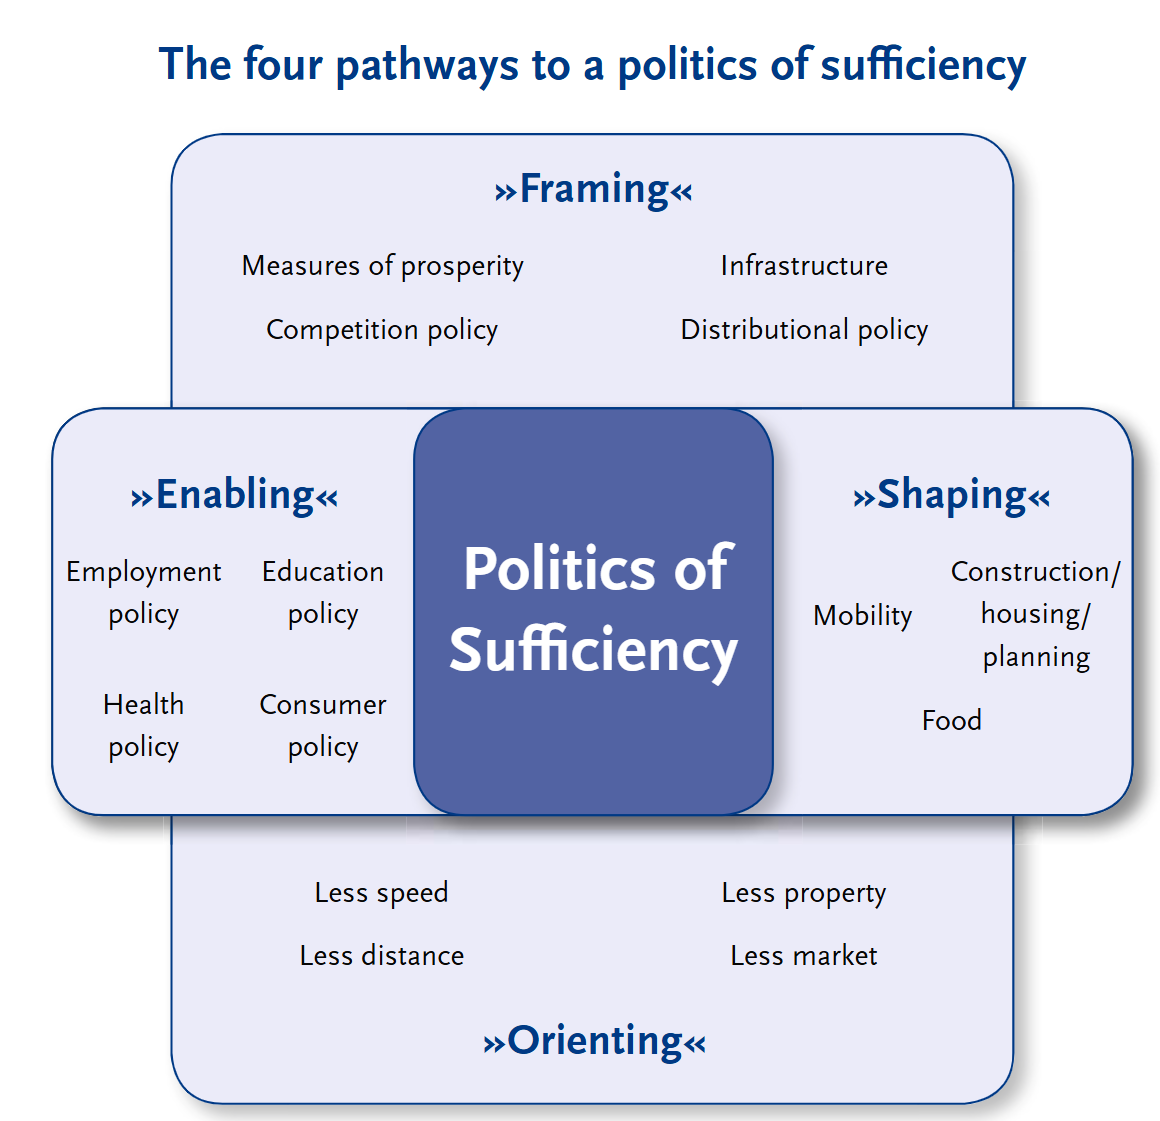
\includegraphics[keepaspectratio]{2_approaches/Images/Fig2_8__PoliticsSufficiency.png}}

}

\caption{\label{fig-development-planetary-boundaries}The four areas of a
politics of sufficiency. (Source: Schneidewind \& Zahrnt (2014))}

\end{figure}%

A policy to promote sufficiency can actively shape our choices, through
attractive sufficiency-oriented offers and services. It can also foster
awareness and provide guidance for adopting sufficiency-oriented
lifestyles and practices. This comprehensive approach aims to shift
consumption towards what is necessary and meaningful, ultimately
reducing excessive resource use.

\subsection{Conclusion}\label{conclusion-4}

Post-growth debates analyse and criticize modern society's dependency on
economic growth, and the negative environmental and social effects of
this growth. Rather than focus solely on technological progress and
market forces, post-growth society theories strive for changes in
society, structures, and institutional frameworks. Overall, post-growth
debates emphasize the need for sustainable approaches to achieve a
comprehensive transformation of the economy and society. Transformation
to a post-growth society requires a reorientation of values, structures,
and institutional frameworks. The challenge is to find ways to shape the
transition to an economy independent of growth, while at the same time
ensuring social justice and ecological sustainability.

Critics of post-growth debates argue that a rejection of economic growth
could have a negative impact on prosperity and social progress. They
fear that an economy independent of growth could lead to stagnating
innovation, fewer jobs, and falling living standards. And they point out
that a negative attitude towards economic growth can have potential
negative effects. Constructively addressing the challenges of growth and
developing viable alternatives are important aspects of enabling
sustainable and equitable change.

\section{\texorpdfstring{\textbf{Indicators for Sustainable Development:
From Principles to
Practice}}{Indicators for Sustainable Development: From Principles to Practice}}\label{indicators-for-sustainable-development-from-principles-to-practice}

A key concern of sustainable development is the ability to
systematically make visible both progress and setbacks---on global,
national, and local levels. Indicators play a crucial role in this
effort: they help capture complex socio-ecological realities, enable
comparability, and support evidence-based policymaking. Precisely
because sustainability is a normative objective, particular attention
must be paid to the selection, design, and use of indicators.

Importantly, indicators are not purely technical measurement tools. They
inevitably reflect specific values, worldviews, and political goals.
Their significance is not solely based on ``objective data'', but also
on decisions about what should be measured, how, and for what purpose.
For instance, Gross Domestic Product (GDP) has long dominated as the
main benchmark for economic success---despite ignoring ecological
damage, social inequality, unpaid care work, and ecosystem services.

In sustainability science and environmental policy, a useful distinction
has emerged between different types of indicators, each serving a
specific function (Vries, 2024):

\begin{itemize}
\item
  \textbf{State indicators} describe the condition of a system or
  resource---such as CO₂ concentration in the atmosphere, the proportion
  of protected forest area, or average life expectancy. These are
  primarily used to monitor trends and system states.
\item
  \textbf{Causal indicators} capture underlying drivers or influencing
  factors that lead to changes within a system. These include, for
  example, fossil fuel consumption or socio-economic drivers like
  urbanization rates or consumption patterns.
\item
  \textbf{Input or intervention indicators} refer to institutional or
  policy measures that are introduced in response to problems. Examples
  include subsidies for renewable energy, legal regulations, or public
  awareness campaigns. They track the presence and nature of
  interventions.
\item
  \textbf{Performance or output indicators} measure the results or
  impacts of these interventions in relation to predefined goals. These
  may include emission reductions, the share of recycled materials, or
  progress in social justice.
\end{itemize}

This classification illustrates that individual indicators often lack
significance in isolation. It is the interaction of indicators---e.g.,
within impact models or causal frameworks---that enables a robust
assessment of sustainability trends and policy responses.

Over the past decades, a wide range of alternative indicator systems has
been developed to provide a more comprehensive picture of societal
development beyond GDP. These approaches aim to integrate economic,
social, and environmental dimensions while making distributional and
non-market contributions visible.

A significant milestone was the development of the \textbf{Human
Development Index (HDI)} by the United Nations Development Programme
(UNDP) in the 1990ies. The HDI combines three dimensions: life
expectancy at birth (as a proxy for health), average and expected years
of schooling (education), and per capita income adjusted for purchasing
power (material living standard). The HDI sought to broaden the narrow
monetary focus of GDP by offering a capability-based understanding of
development as ``the expansion of people's choices'' (Sen, 1999). Today,
it remains a standard reference in development economics (see UNDP Human
Development Reports since 1990).

A more advanced approach is the \textbf{Genuine Progress Indicator
(GPI)}, which starts with personal consumption (as GDP does) but adjusts
for external costs such as environmental degradation, resource use,
crime, and income inequality to reveal trade-offs between costs and
benefits of economic growth. It also adds value for unpaid services like
domestic work and volunteering. First proposed by Daly and Cobb (1989)
as Sustainable Economic Welfare (ISEW), the GPI is well established in
ecological economics (see Talberth et al., 2007). Unlike GDP, which
typically increases over time, the GPI has stagnated or declined in many
high-income countries since the 1980s---indicating a possible decoupling
between growth and well-being.

\begin{figure}[H]

\centering{

\pandocbounded{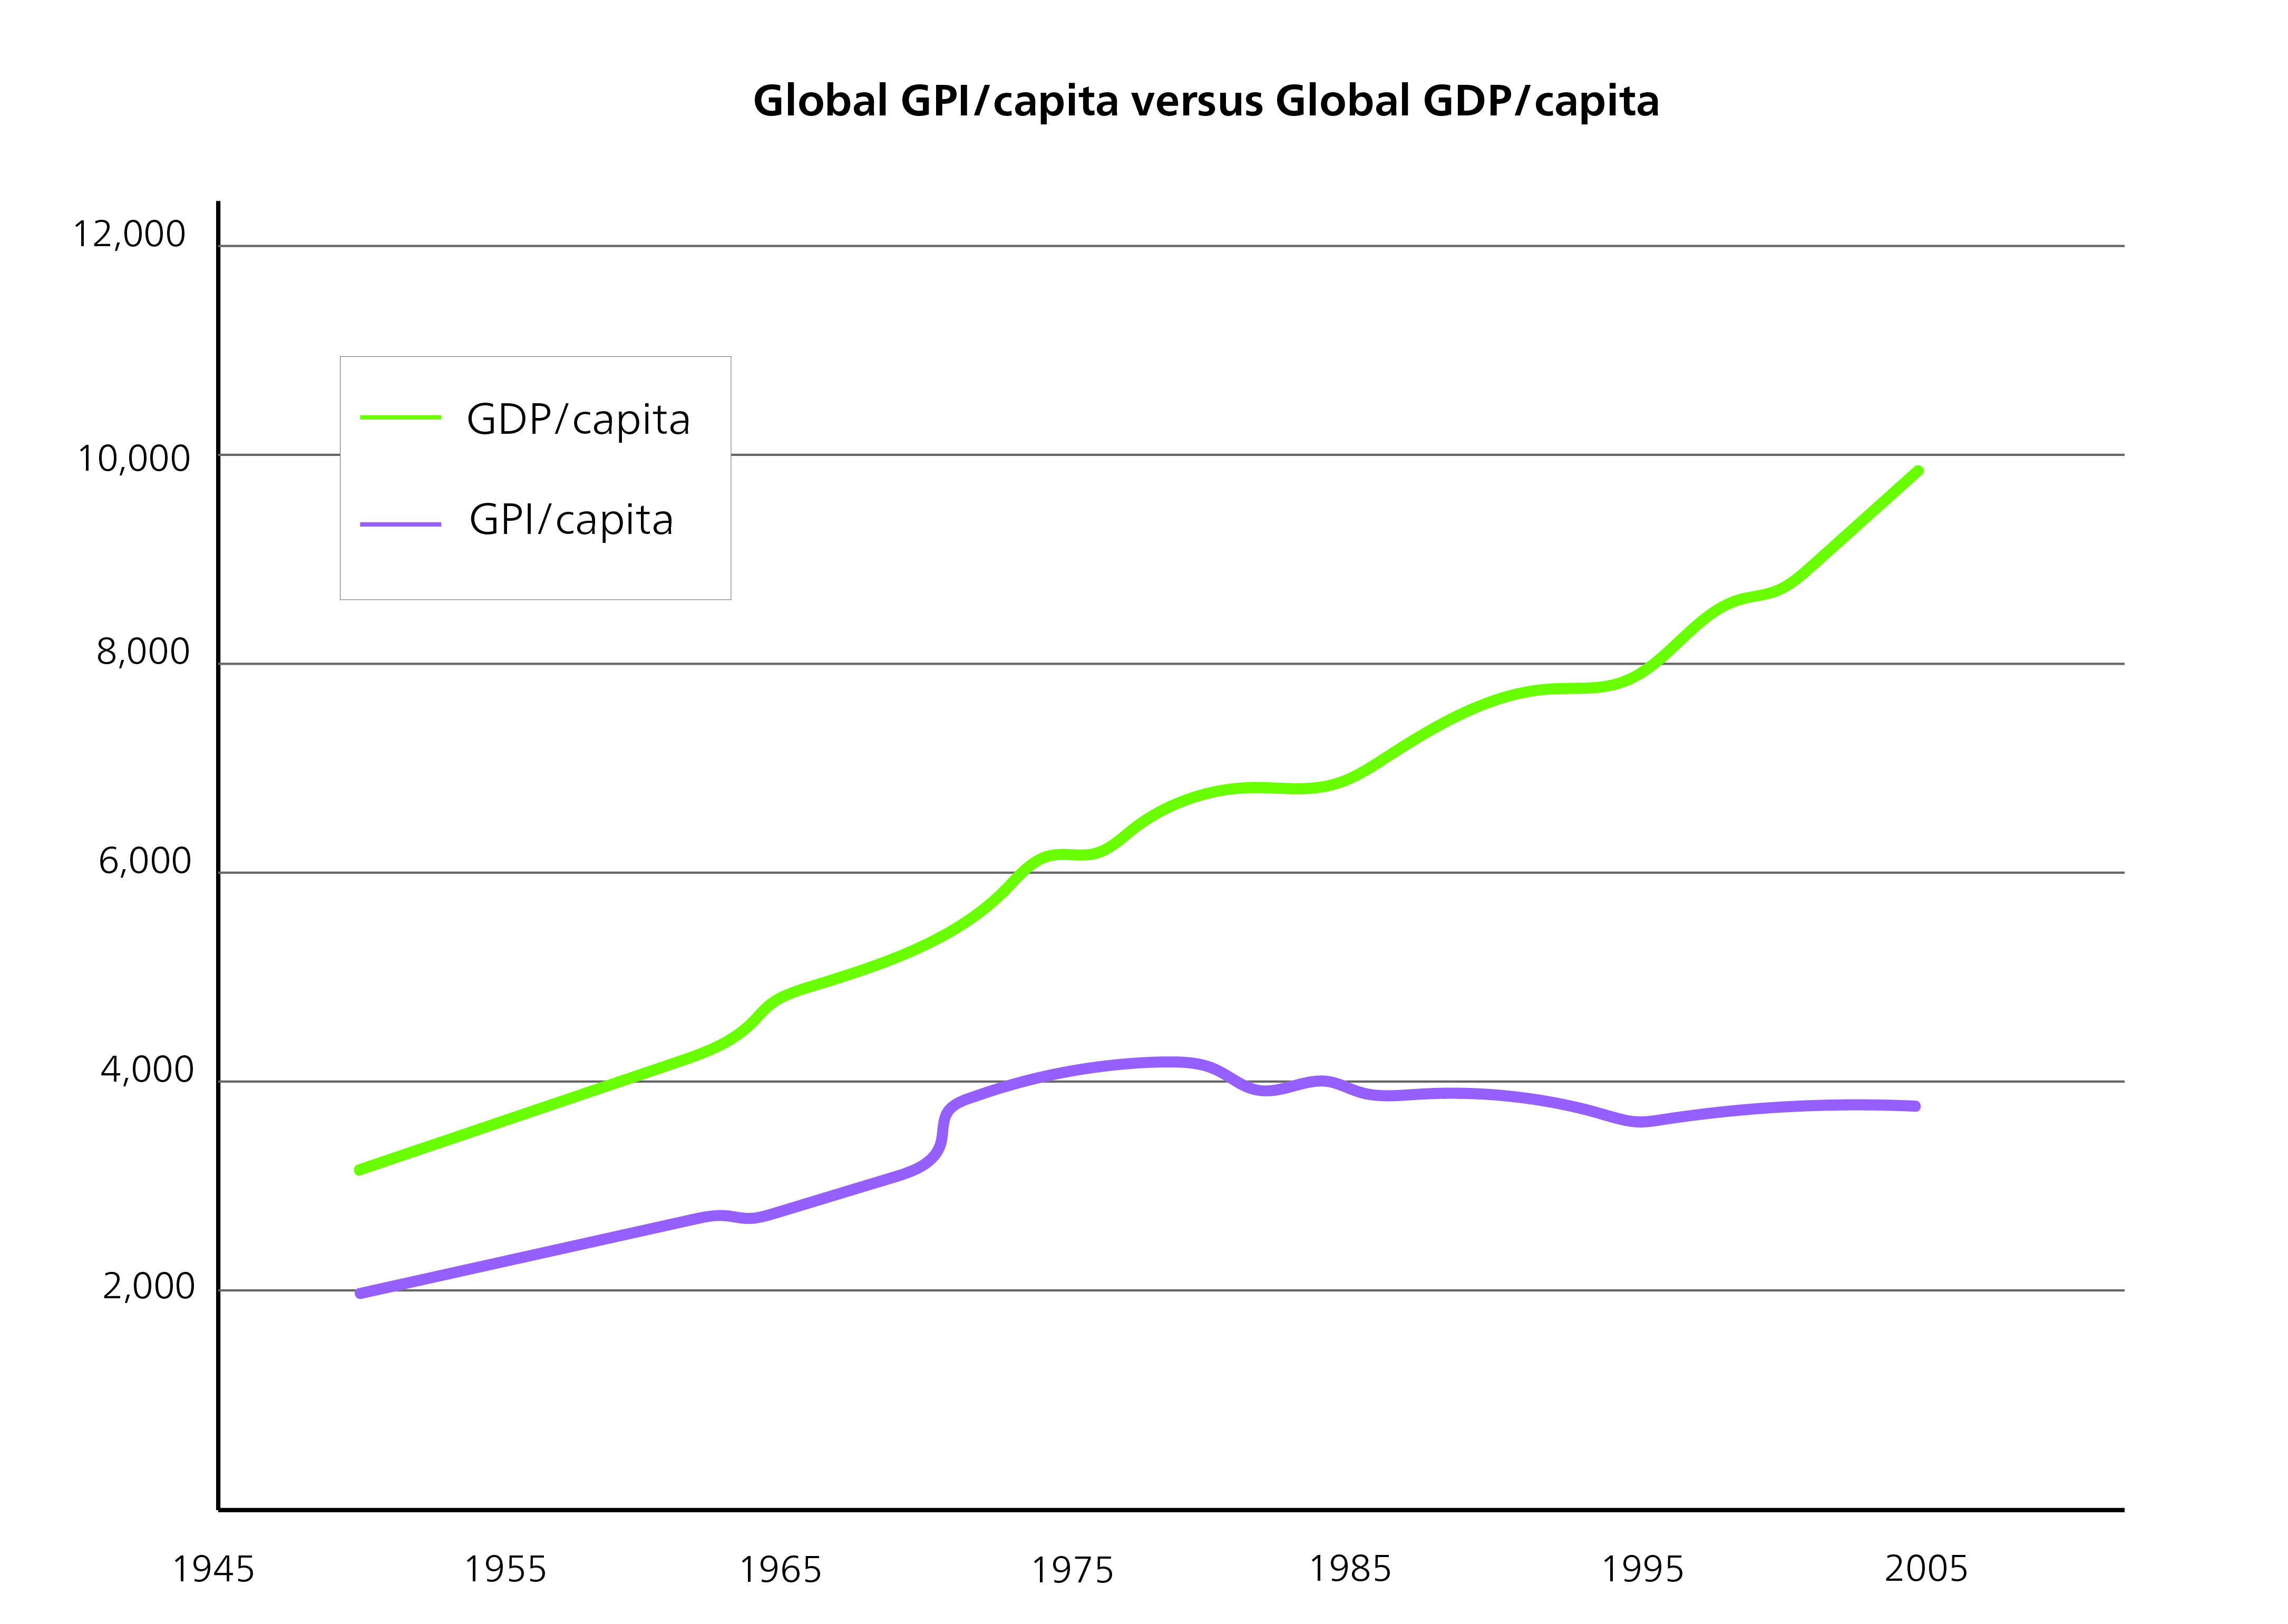
\includegraphics[keepaspectratio]{2_approaches/Images/Fig2_9__GDPxGPI.jpg}}

}

\caption{\label{fig-GDPxGPI}Comparison of global Gross Domestic Product
(GDP) and Genuine Progress Indicator (GPI) (Source: Own ilustration)}

\end{figure}%

Another commonly used measure is the \textbf{Ecological Footprint},
which translates human resource use into global hectares. It represents
the biologically productive area needed to meet the resource demand of
an individual, region, or country---including land for food production,
settlement, and carbon absorption. Developed by Wackernagel and Rees
(1996) and promoted by the Global Footprint Network, it is especially
prevalent in environmental education. The Ecological Footprint
illustrates whether a population is living within its ecological
means---i.e., whether it exceeds its fair share of global biocapacity.

\begin{figure}[H]

\centering{

\pandocbounded{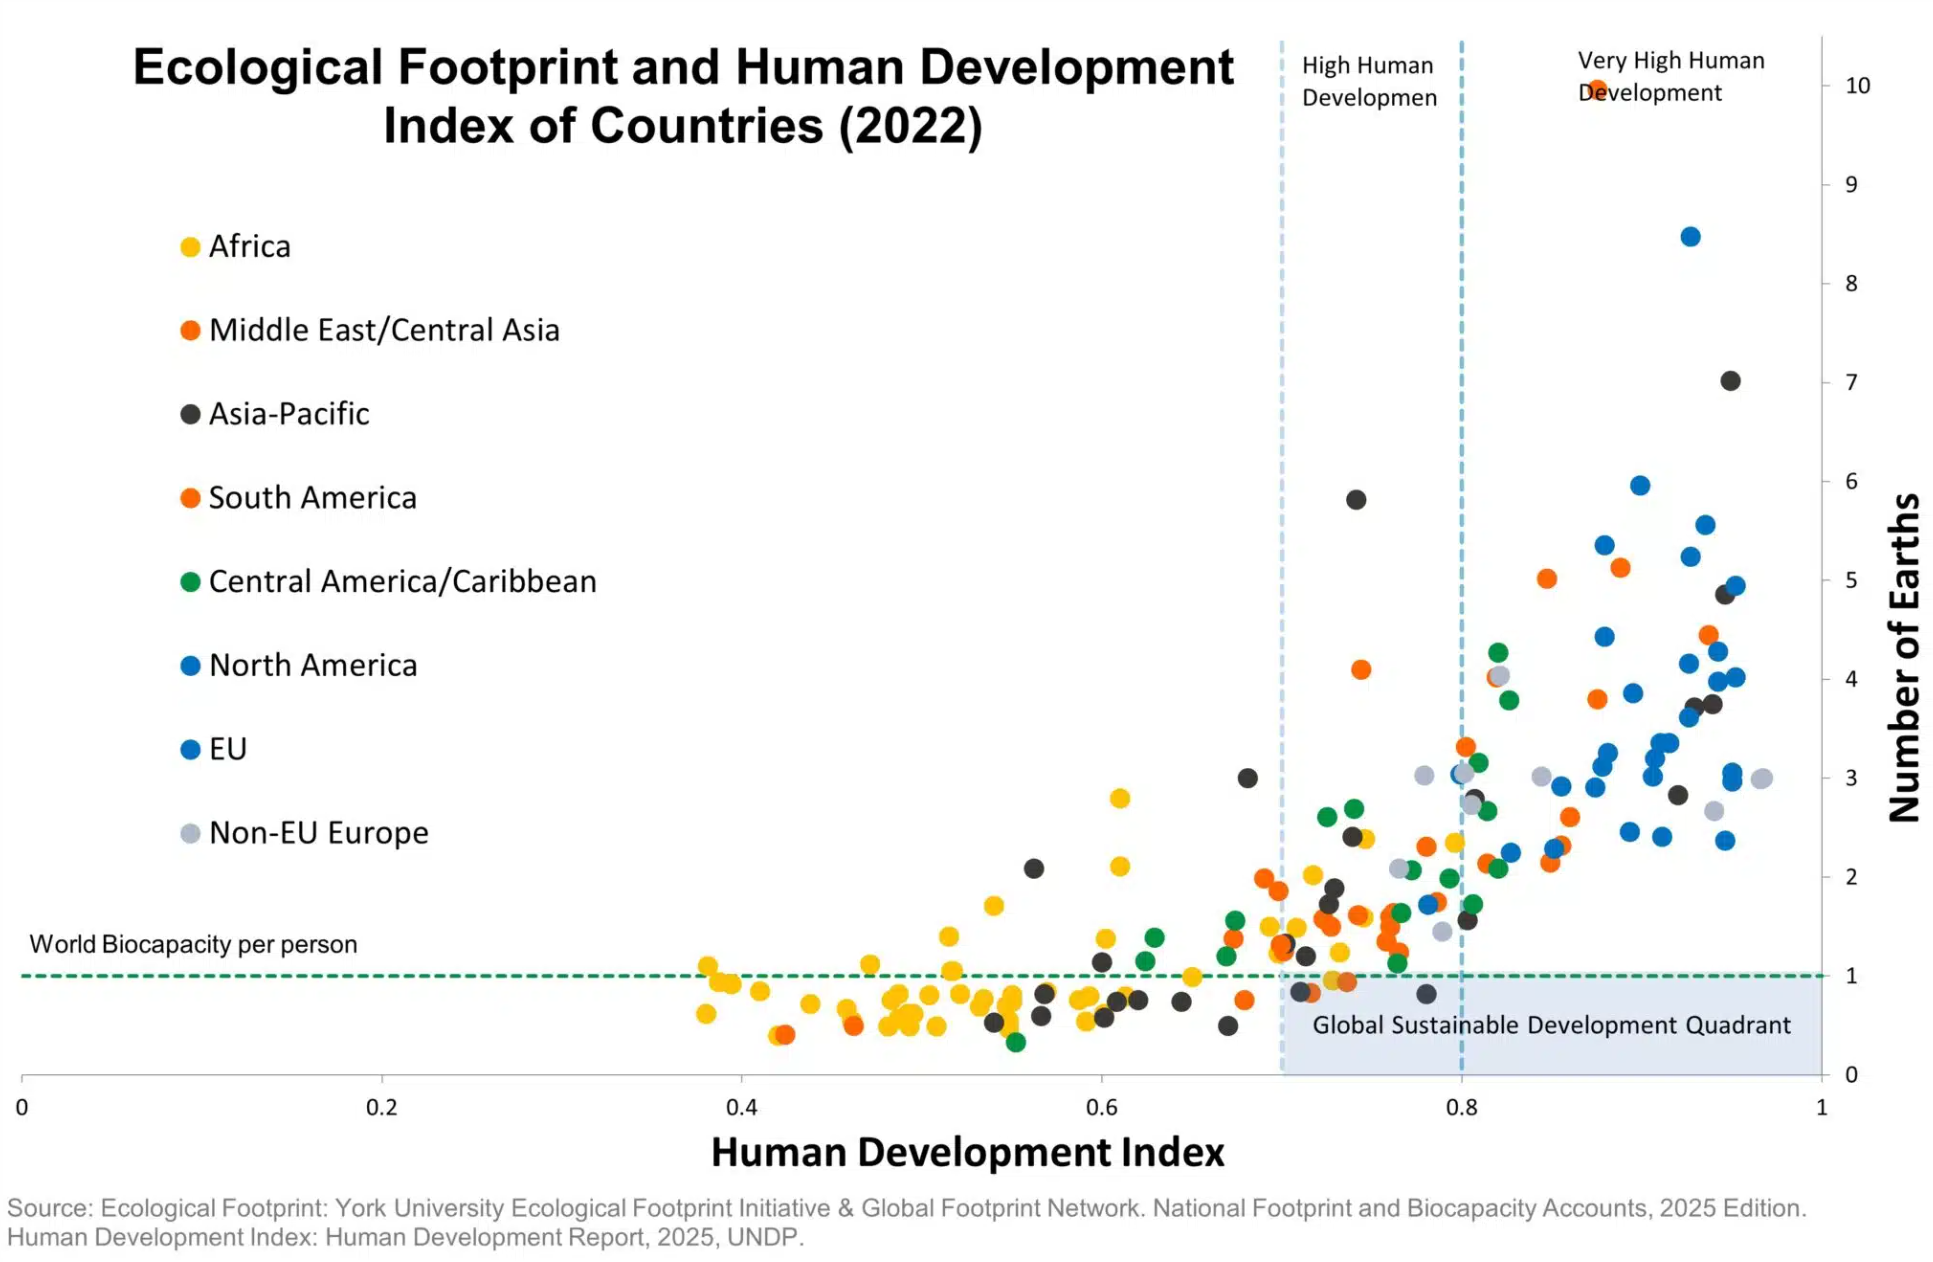
\includegraphics[keepaspectratio]{2_approaches/Images/Fig2_10__EcoFootprintHDI.png}}

}

\caption{\label{fig-EcoFootprintHDI}Correlation between Ecological
Footprint and Human Development Index (Source: x)}

\end{figure}%

The \textbf{Happy Planet Index (HPI)} offers a more subjective approach,
combining life satisfaction (survey-based), life expectancy, and
ecological footprint to calculate ``wellbeing per unit of environmental
input''. Developed by the New Economics Foundation, the HPI shows that
high life satisfaction does not necessarily require high resource
consumption. Middle-income countries like Costa Rica often score higher
than industrialized nations with unsustainable consumption patterns
(NEF, 2006).

In the German-speaking world, the \textbf{National Welfare Index (NWI)}
has been introduced as a GPI-based tool adapted to national data
availability. It includes dimensions such as income distribution,
environmental burden, and health costs. Initially developed by the
Institute for Ecological Economy Research (IÖW) and the Environmental
Policy Research Centre (FFU) at FU Berlin, the NWI has been tested in
several German federal states (Diefenbacher \& Zieschank, 2011).

Another particularly relevant measure is the \textbf{Multidimensional
Poverty Index (MPI)}, developed by the Oxford Poverty and Human
Development Initiative (OPHI) in collaboration with the UNDP. It
captures poverty across three core dimensions: health, education, and
standard of living. Indicators include child mortality, school
attendance, access to electricity, and housing conditions. Unlike
income-based measures, the MPI provides a nuanced understanding of
deprivation across overlapping dimensions. Bader et al.~(2017)
demonstrate the value of the MPI in a longitudinal study on poverty in
the Lao PDR, showing how rapid economic growth reduced income poverty
while simultaneously exacerbating disparities in education,
infrastructure, and health access.

\begin{tcolorbox}[enhanced jigsaw, left=2mm, arc=.35mm, titlerule=0mm, opacityback=0, leftrule=.75mm, title={Tip}, breakable, bottomtitle=1mm, rightrule=.15mm, coltitle=black, toptitle=1mm, bottomrule=.15mm, colback=white, opacitybacktitle=0.6, colbacktitle=quarto-callout-tip-color!10!white, toprule=.15mm, colframe=quarto-callout-tip-color-frame]

\textbf{The Ecological Footprint -- Explanation and Critique}

The \textbf{Ecological Footprint} measures how much biologically
productive land and sea area (in global hectares) is required to sustain
the resource use of an individual, population, or country over time. It
includes land required for CO₂ absorption, food production,
infrastructure, and other human needs. The concept was developed in the
1990ies by Mathis Wackernagel and William Rees and has become one of the
most widely recognized tools for environmental communication.

The Ecological Footprint is often used in public awareness campaigns,
notably in connection with the annually published \emph{Earth Overshoot
Day}---the symbolic date when humanity's resource consumption exceeds
Earth's capacity to regenerate those resources in the same year.

\end{tcolorbox}

\textbf{Main limitations of the indicator based on EEA (2020):}

\begin{itemize}
\item
  Non-ecological aspects of sustainability: having a footprint smaller
  than the biosphere is a necessary minimum condition for a sustainable
  society, but it is not sufficient. For instance, the ecological
  footprint does not consider social well-being. In addition, on the
  resource side, even if the ecological footprint is within biocapacity,
  poor management can still lead to depletion. A footprint smaller than
  biocapacity is merely a necessary condition for making quality
  improvements replicable and scalable.
\item
  Depletion of non-renewable resources: the footprint does not track the
  amount of non-renewable resource stocks, such as oil, natural gas,
  coal or metal deposits. The footprint associated with these materials
  is based on the regenerative capacity used or compromised by their
  extraction and, in the case of fossil fuels, the area required to
  assimilate the wastes they generate.
\item
  Inherently unsustainable activities: activities that are inherently
  unsustainable, such as the release of heavy metals, radioactive
  materials and persistent synthetic compounds (e.g.~chlordane,
  polychlorinated biphenyls (PCBs), chlorofluorocarbons (CFCs),
  polyvinyl chloride (PVC), dioxins, etc.), do not enter directly into
  footprint calculations. These are activities that need to be phased
  out independently of their quantity (there is no biocapacity budget
  for using them). Where these substances cause a loss of biocapacity,
  however, their influence can be seen.
\item
  Ecological degradation: the footprint does not directly measure
  ecological degradation, such as increased soil salinity from
  irrigation, which could affect future bioproductivity. However, if
  degradation leads to reductions in bioproductivity, then this loss is
  captured when measuring biocapacity in the future. Moreover, by
  looking at only the aggregate figure, `under-exploitation' in one area
  (e.g.~forests) can hide over-exploitation in another area
  (e.g.~fisheries).
\item
  Resilience of ecosystems: footprint accounts do not identify where and
  in what way the capacity of ecosystems are vulnerable or resilient.
  The footprint is merely an outcome measure documenting how much of the
  biosphere is being used compared with how productive it is.
\end{itemize}

Despite these limitations, the Ecological Footprint remains a useful
entry point for engaging broader audiences in discussions on global
ecological justice and planetary responsibility---especially in
educational and communication settings.

\section{\texorpdfstring{\textbf{Between Simplification and Complexity:
Interactions Between
SDGs}}{Between Simplification and Complexity: Interactions Between SDGs}}\label{between-simplification-and-complexity-interactions-between-sdgs}

A central challenge in designing sustainability indicators lies in
balancing simplification with complexity. Indicators are intended to
support decision-making, yet must account for a wide array of
interactions, uncertainties, and contextual dependencies.

This is particularly evident in the 2030 Agenda for Sustainable
Development. While the Agenda includes 17 distinct goals and numerous
sub-targets, these goals do not exist in isolation. Rather, they are
intricately interconnected: progress in one area may reinforce,
neutralize, or hinder progress in another. Consequently, indicators that
illuminate these relationships are essential for coherent policy design.

Breu et al.~(2020) present a methodology based on the interactions
framework developed by Nilsson et al.~(2016), which systematically
classifies the relationships between SDGs on a seven-point scale: from
strongly negative (--3) to strongly positive (+3). They applied this
approach to Switzerland's national sustainability framework, revealing
areas where policy actions toward one SDG may support or conflict with
others. For example, measures to reduce poverty (SDG 1) could conflict
with biodiversity goals (SDG 15) if not designed to be environmentally
sustainable.

\part{Transforming (Un-)sustainable systems: Key areas and strategic
approaches}

\chapter{Environmental
Sustainability}\label{environmental-sustainability}

The economy is integral not only to society, but also to nature. Humans
are living beings and therefore reliant on material resources to fulfill
their needs. They also require intact ecosystems and a climate suitable
for human habitation. When we speak of ``environmental sustainability'',
we generally mean the protection of the diversity and functioning of
natural ecosystems and the services they provide for future generations.
This is an anthropocentric definition, as it focuses on human activities
and how these seek to ensure the long-term sustainability of nature for
human benefit. This perspective is also reflected in our everyday
language and our dualistic separation of ``human'' and ``environment'',
a separation that goes back to the 19th century and persists to this
day. For example, we separate science into ``natural science'' and
``social science'', and our analyses often conceptualize environmental
damage as ``externalities''. Another understanding of environmental
sustainability emphasizes the importance of maintaining the
self-regulation of the Earth's climate system. This view highlights the
interaction and feedback between various components of the Earth's
climate system.

\section{The normative dimension of environmental
sustainability}\label{the-normative-dimension-of-environmental-sustainability}

Although our understanding of how ecosystems work is based on thoroughly
researched empirical information (and therefore constitutes ``systems
knowledge''), environmental sustainability remains a normative concept.
This means that it is based not only on scientific findings, but also on
an ethical evaluation (Figure~\ref{fig-normative-dimension}). The
various interpretations of environmental sustainability offer different
answers to the question of what should be preserved, and why. Each
approach to environmental sustainability therefore expresses the desired
state of the ecological environment, both now and in the future -- what
aspects of nature should be preserved or survive from the present to the
future. For example, when we talk about ecosystem services, the
intention is often to preserve ecosystems in a way that continues to
support and maintain our own welfare (in this sense, it is an
anthropocentric perspective).

\begin{figure}[H]

\centering{

\pandocbounded{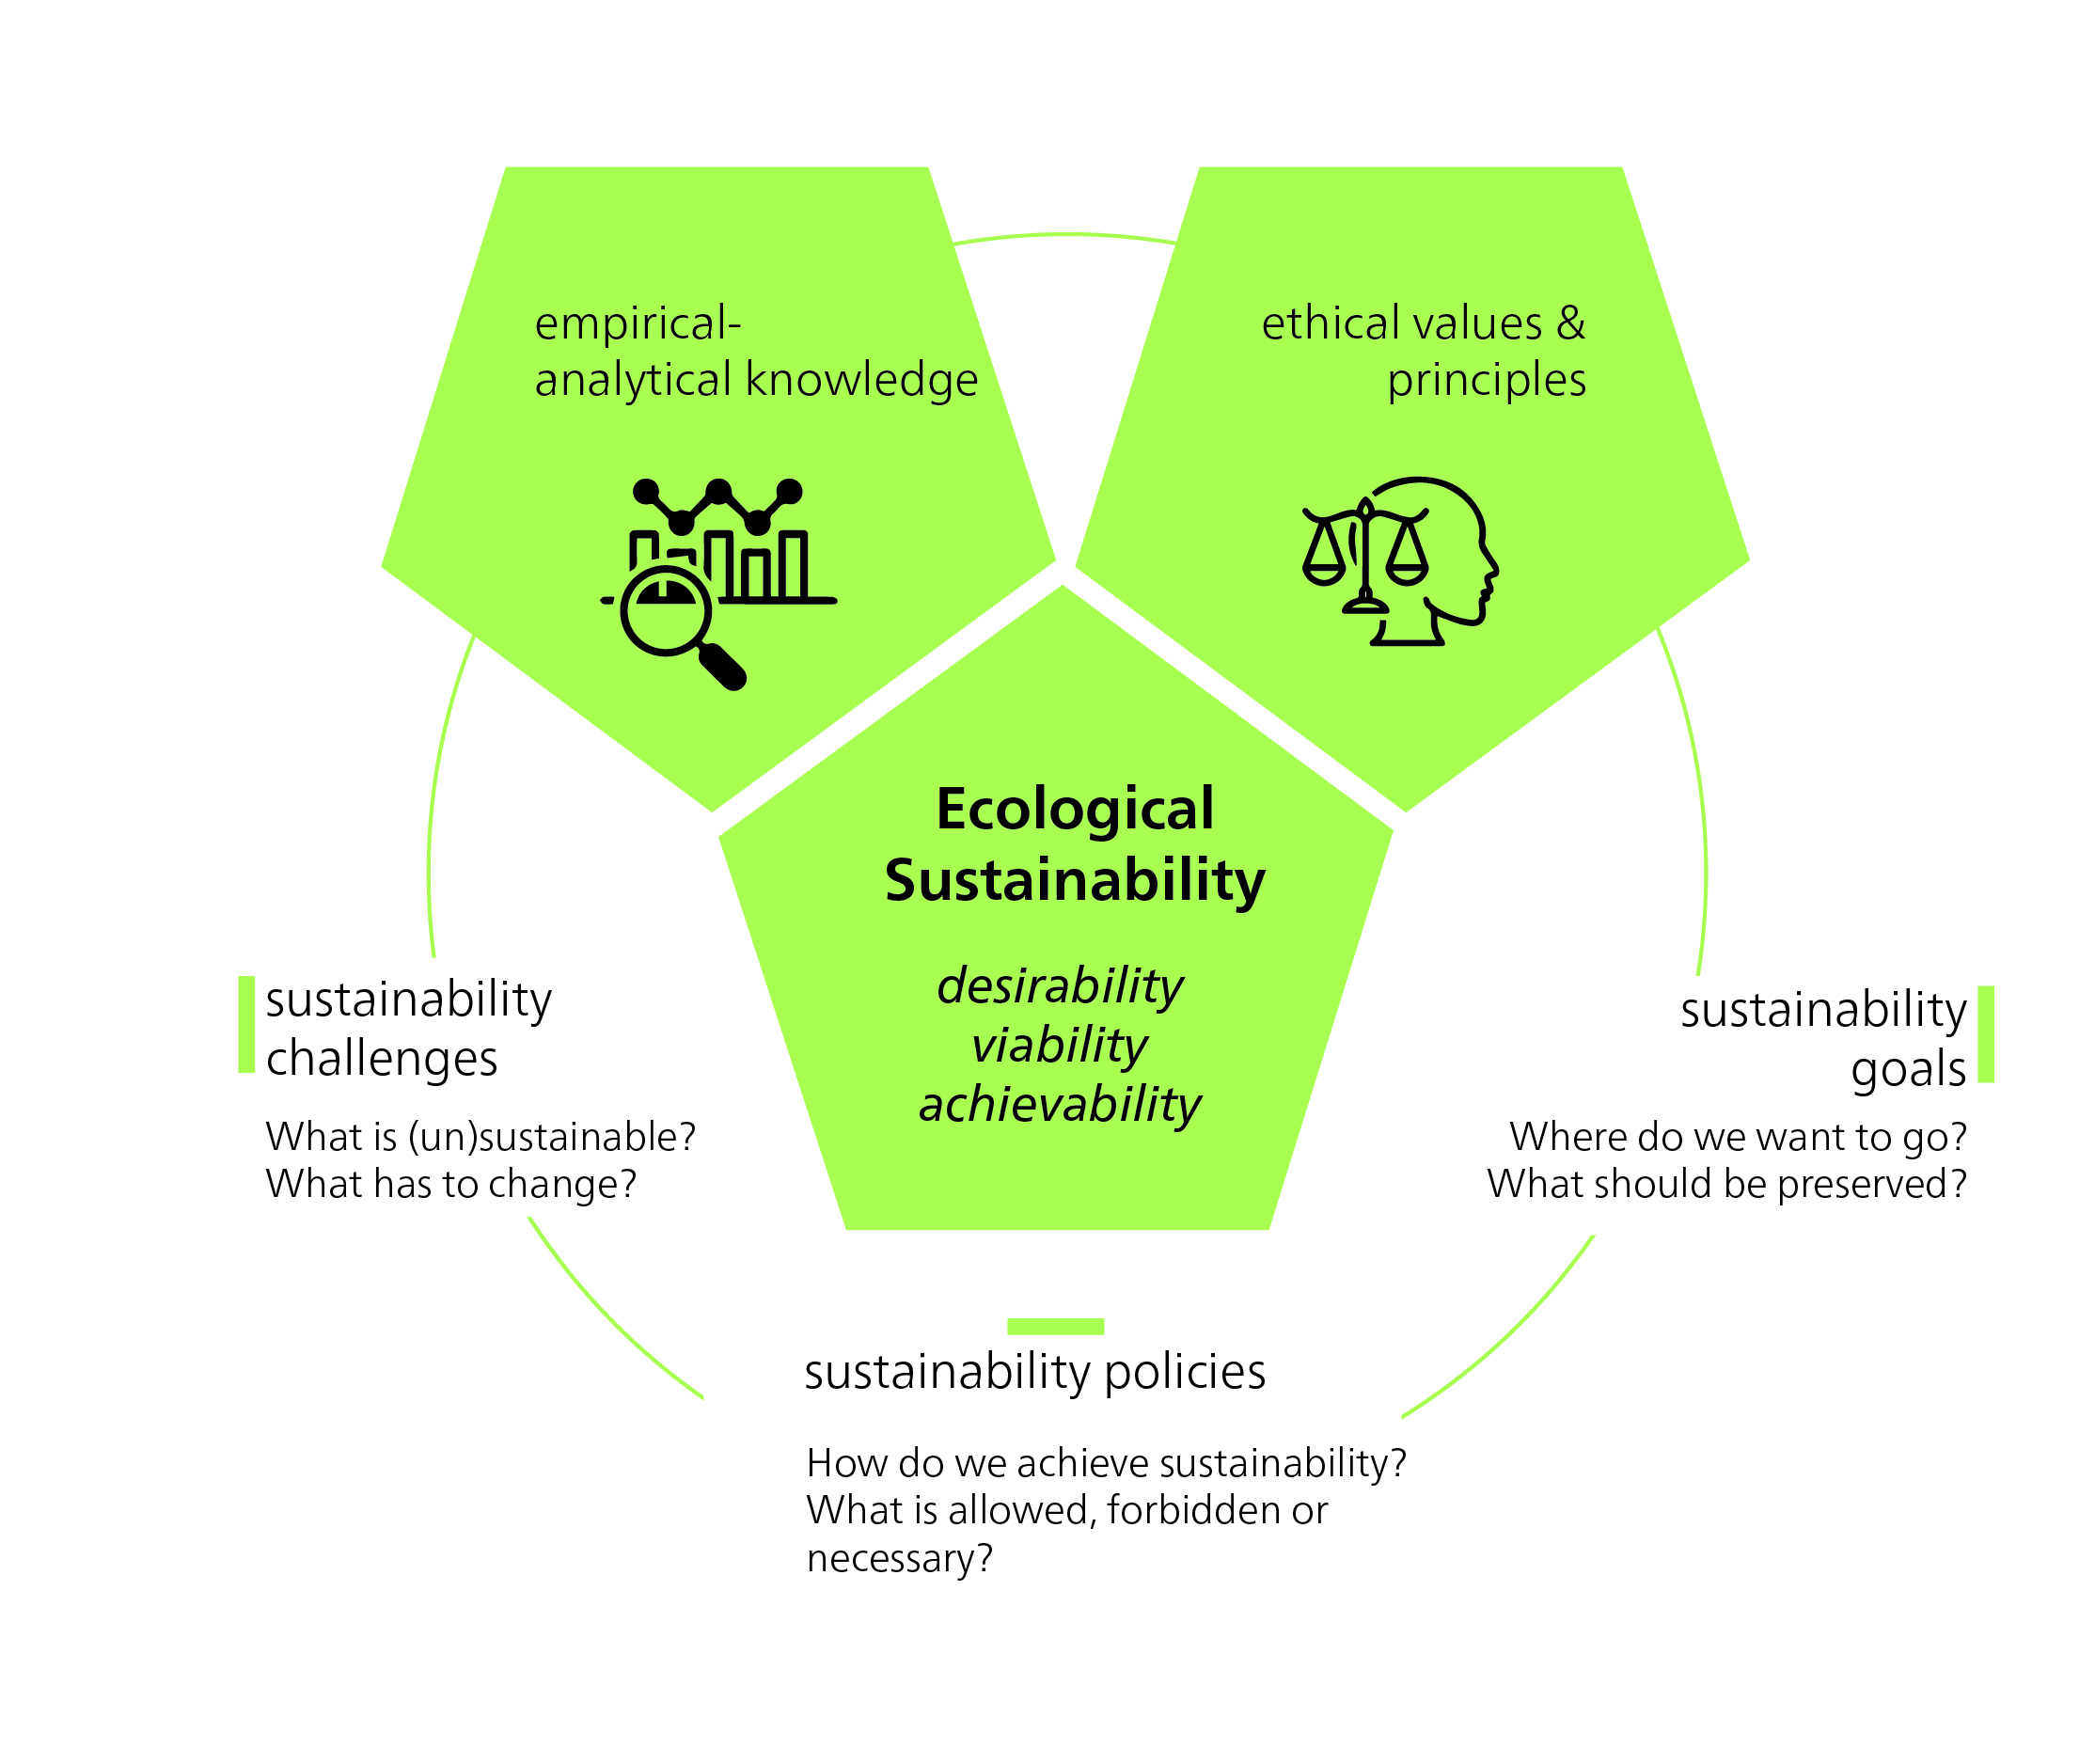
\includegraphics[keepaspectratio]{3_ecological-sustainability/images/Images_en/Fig3_1__NEecology.jpg}}

}

\caption{\label{fig-normative-dimension}The normative dimension of
environmental sustainability (Source:Own illustration) .}

\end{figure}%

Ethical judgments and justifications shape which ecological properties
and functions we preserve for future generations, and which we deem
intrinsically valuable in nature. What constitutes a desirable state for
ecosystems, and why? What aspects of the ecological environment deserve
protection, and what is the aim of this protection? Is it necessary to
keep ecosystems as pristine as possible, and how do we define
``naturalness''? To what extent should we use ecosystems for human
purposes without restriction, and are there areas that we should leave
for organisms to use, with minimum human intervention? Interpretations
of environmental sustainability depend on the goals being pursued: for
whom, why, and how (Figure~\ref{fig-normative-dimension}).

\begin{tcolorbox}[enhanced jigsaw, left=2mm, arc=.35mm, titlerule=0mm, opacityback=0, leftrule=.75mm, title={Tip}, breakable, bottomtitle=1mm, rightrule=.15mm, coltitle=black, toptitle=1mm, bottomrule=.15mm, colback=white, opacitybacktitle=0.6, colbacktitle=quarto-callout-tip-color!10!white, toprule=.15mm, colframe=quarto-callout-tip-color-frame]

\textbf{Specific examples of ethical assessments in the context of
environmental sustainability}

Wildlife conservation: Should we intervene in natural wildlife
populations to protect endangered species and maintain the balance of
ecosystems? Or should we leave nature as untouched as possible, even if
this means losing some species?

Biotechnological interventions: Is it morally acceptable to use
biotechnological methods, such as genetic engineering, to alter the
ecological characteristics of organisms and potentially influence
ecosystems?

Conservation of endangered species: Should we focus on protecting and
preserving endangered species to maintain biodiversity, or should we
focus on preserving broadly available species that are more important
for the human diet or the economy?

Protecting ecosystems: Should we establish protected areas to preserve
threatened ecosystems and species, even if this restricts local
communities in their economic activities? How can we strike a balance
between conservation and sustainable use?

\end{tcolorbox}

\section{Ecosystems, Ecosystem management, and Ecosystem
services}\label{ecosystems-ecosystem-management-and-ecosystem-services}

An ecosystem is a group of living organisms and their physical
surroundings that interact with each other. Ecosystems can range from
small, like a flowerpot, to large, like an ocean. When similar
ecosystems are found in a larger region with the same climate, they are
called biomes. Energy and material flows are important for the
functioning of an ecosystem. Some of these flows, such as the carbon
cycle, take place at the global level, while others are more localized.
Most ecosystems obtain their energy from the sun and can influence the
Earth's climate through their interactions (Quelle: Britannica).

Ecosystem services are the benefits that humans derive from ecosystems
such as mangrove forests, oceans, or wetlands. The services provided by
ecosystems include the provision of clean water, the prevention of
flooding, the promotion of crop growth, and the provision of places for
leisure activities. The Millenium Ecosystem Assessment, published in
2005, divides ecosystem services into four categories (cf.~green Box in
Figure~\ref{fig-ecosystem}): \emph{provisioning services},
\emph{regulating services}, \emph{cultural services}, and
\emph{supporting services} (Quelle:MEA, 2005). Note that the supporting
services, which are primarily fundamental biophysical processes, enable
and guarantee the other services in the first place.

\begin{figure}[H]

\centering{

\pandocbounded{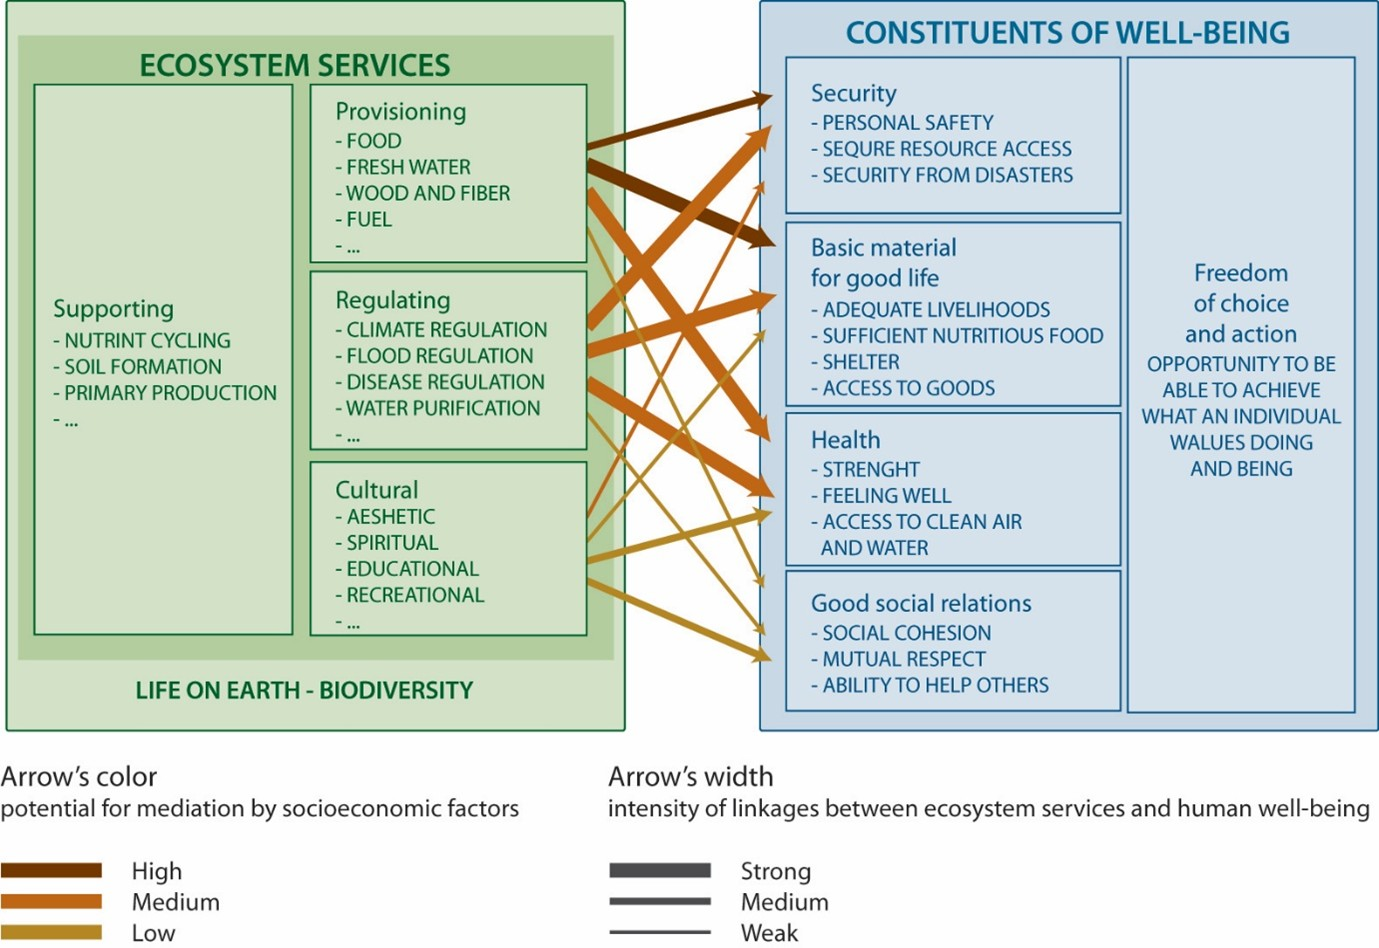
\includegraphics[keepaspectratio]{3_ecological-sustainability/images/Images_en/Fig3_2__Ecosystem.jpg}}

}

\caption{\label{fig-ecosystem}Millennium Ecosystem Assessment (Source:
The Millenium Ecosystem Assessment)}

\end{figure}%

According to the Millennium Ecosystem Assessment, these ecosystem
services can improve our quality of life and our economy (cf.~blue Box
in Figure~\ref{fig-ecosystem}). While this way of looking at ecosystems
views humans as separate from the environment, it emphasizes the
relevance of ecosystem services for human well-being. Ultimately, the
concept of ecosystem services seeks to place greater consideration on
the value of nature in policy and economic decisions. However, the
ecosystem services concept also plays a role in landscape and spatial
planning. For example, it's used to analyse how spatially effective
(legal) regulations impact ecosystem services, and consequently, human
well-being (Quelle: cf.~Albert et al.~2016).

\begin{tcolorbox}[enhanced jigsaw, left=2mm, arc=.35mm, titlerule=0mm, opacityback=0, leftrule=.75mm, title={Tip}, breakable, bottomtitle=1mm, rightrule=.15mm, coltitle=black, toptitle=1mm, bottomrule=.15mm, colback=white, opacitybacktitle=0.6, colbacktitle=quarto-callout-tip-color!10!white, toprule=.15mm, colframe=quarto-callout-tip-color-frame]

\textbf{Case study: Ecosystem services in Madagascar}

This landscape on the eastern coast of Madagascar offers a case study
for ecosystem services. Ecosystem services in this area include
firewood, which is used by local inhabitants for cooking, and rice,
which is a staple food. Describing agricultural products such as these
as ecosystem services illustrates that they only become ``services''
through human demand. Ecosystem services are not given in nature per se:
instead, they represent a perspective through which humans view and
describe the environment. Other ecosystem services in this landscape
include the water cycle, which is vital for local inhabitants, as they
rely on rivers for drinking water. Water is also used for agricultural
irrigation and other purposes. Climate regulation is another significant
service, important both locally and globally.

This landscape clearly illustrates that the demand for and importance of
ecosystem services vary among individuals or groups. Such diverse claims
on ecosystem services from the same land can lead to \textbf{conflicts
of interest}. Demand for agricultural products or firewood, for example,
can conflict with climate-regulating and biodiversity-promoting
(international) demands on the rainforest.

\end{tcolorbox}

Humans have had an influence on many ecosystem services, both directly
and indirectly. While these impacts have often been negative, some have
been positive. For example, replacing natural ecosystems with cultivated
agroecosystems has increased the value of ecosystem services for humans.
Take, for example, dry meadows and pastures in Switzerland. Only through
centuries of forest clearing and extensive agricultural use in alpine
locations could the ecosystem services these areas provided (in this
case, fodder production) be used and increased. At the same time, these
anthropogenically influenced sites harboured rare meadow plants and
pollinators, thus fostering a high level of biodiversity. These areas
are also vital for tourism, as they significantly shape the alpine
landscape. Consequently, these extensively used areas generally offer
greater overall ecosystem service multifunctionality than intensively
farmed grasslands (Quelle: Richter et al.~2024).

Many of the negative effects on ecosystems and their services result
directly from human land use and overfishing. In addition, indirect
factors such as climate change and invasive non-native species
significantly impair the stability and functionality of ecosystems. Two
research projects with significant CDE involvement -- Woody Weeds and
Woody Weeds+ -- have demonstrated that invasive woody plants such as
\emph{Prosopis juliflora} have a major impact on biodiversity and local
livelihoods in East Africa. Originally introduced to combat
desertification and timber extraction, this species displaces native
vegetation and is not suitable as animal feed without processing
(\href{https://www.cde.unibe.ch/forschung/projekte/woody_invasive_alien_species_in_eastern_africa/index_ger.html}{CDE}).

\subsection{The monetary valuation of ecosystem
management}\label{the-monetary-valuation-of-ecosystem-management}

The term \emph{nature's services} first appeared in the publication
``How much are Nature's Services Worth?'' (Quelle: Westman, 1977). The
synonymous term ``\emph{ecosystem services}'' was coined a few years
later (Quelle: Ehrlich and Ehrlich, 1981). The concept of ecosystem
services and the thinking behind it are closely linked to economic
philosophy and practice (Quelle: Gómez-Baggethun et al.~2010). Around 20
years after the introduction of ``nature's services'', Robert Costanza
and colleagues estimated that the \textbf{global value of 17 ecosystem
services was worth 33 trillion US dollars per year} (Quelle: Costanza et
al.~1997). A recalculation in 2011 showed that this value had already
fallen by between 4.3 trillion and 20.2 trillion US dollars per year
(Quelle: Costanza et al.~2014). It is predicted that by 2050, the value
of ecosystem services will either drop by up to USD 51 trillion per
year, or rise by up to USD 30 trillion per year, depending on land use
scenario (Quelle: Kubiszewski et al.~2017).

Calculating the \textbf{monetary value of ecosystem services} typically
involves three steps and requires high-quality and differentiated data.
1) The first step is to measure the change in ecosystem services after
an intervention, thus placing the focus not on the status quo, but on
the difference. 2) The second step is to evaluate the impact of this
change on people's socio-economic well-being. 3) The third and final
step is to place a monetary value on the resulting change in
productivity or prosperity (Quelle: \emph{M1 Lecture by} \emph{Astrid
Zabel}). There are \textbf{many different methods for calculating the
monetary value of ecosystem services} (Figure~\ref{fig-monetary-value}).
One such method is ``green accounting'', which uses existing market
values, if available, or exchange values as an approximation
(e.g.~comparing avalanche barriers and protection forests). Another
method is cost--benefit analysis, which can be divided into two types:
stated preferences and revealed preferences.

\begin{figure}[H]

\centering{

\pandocbounded{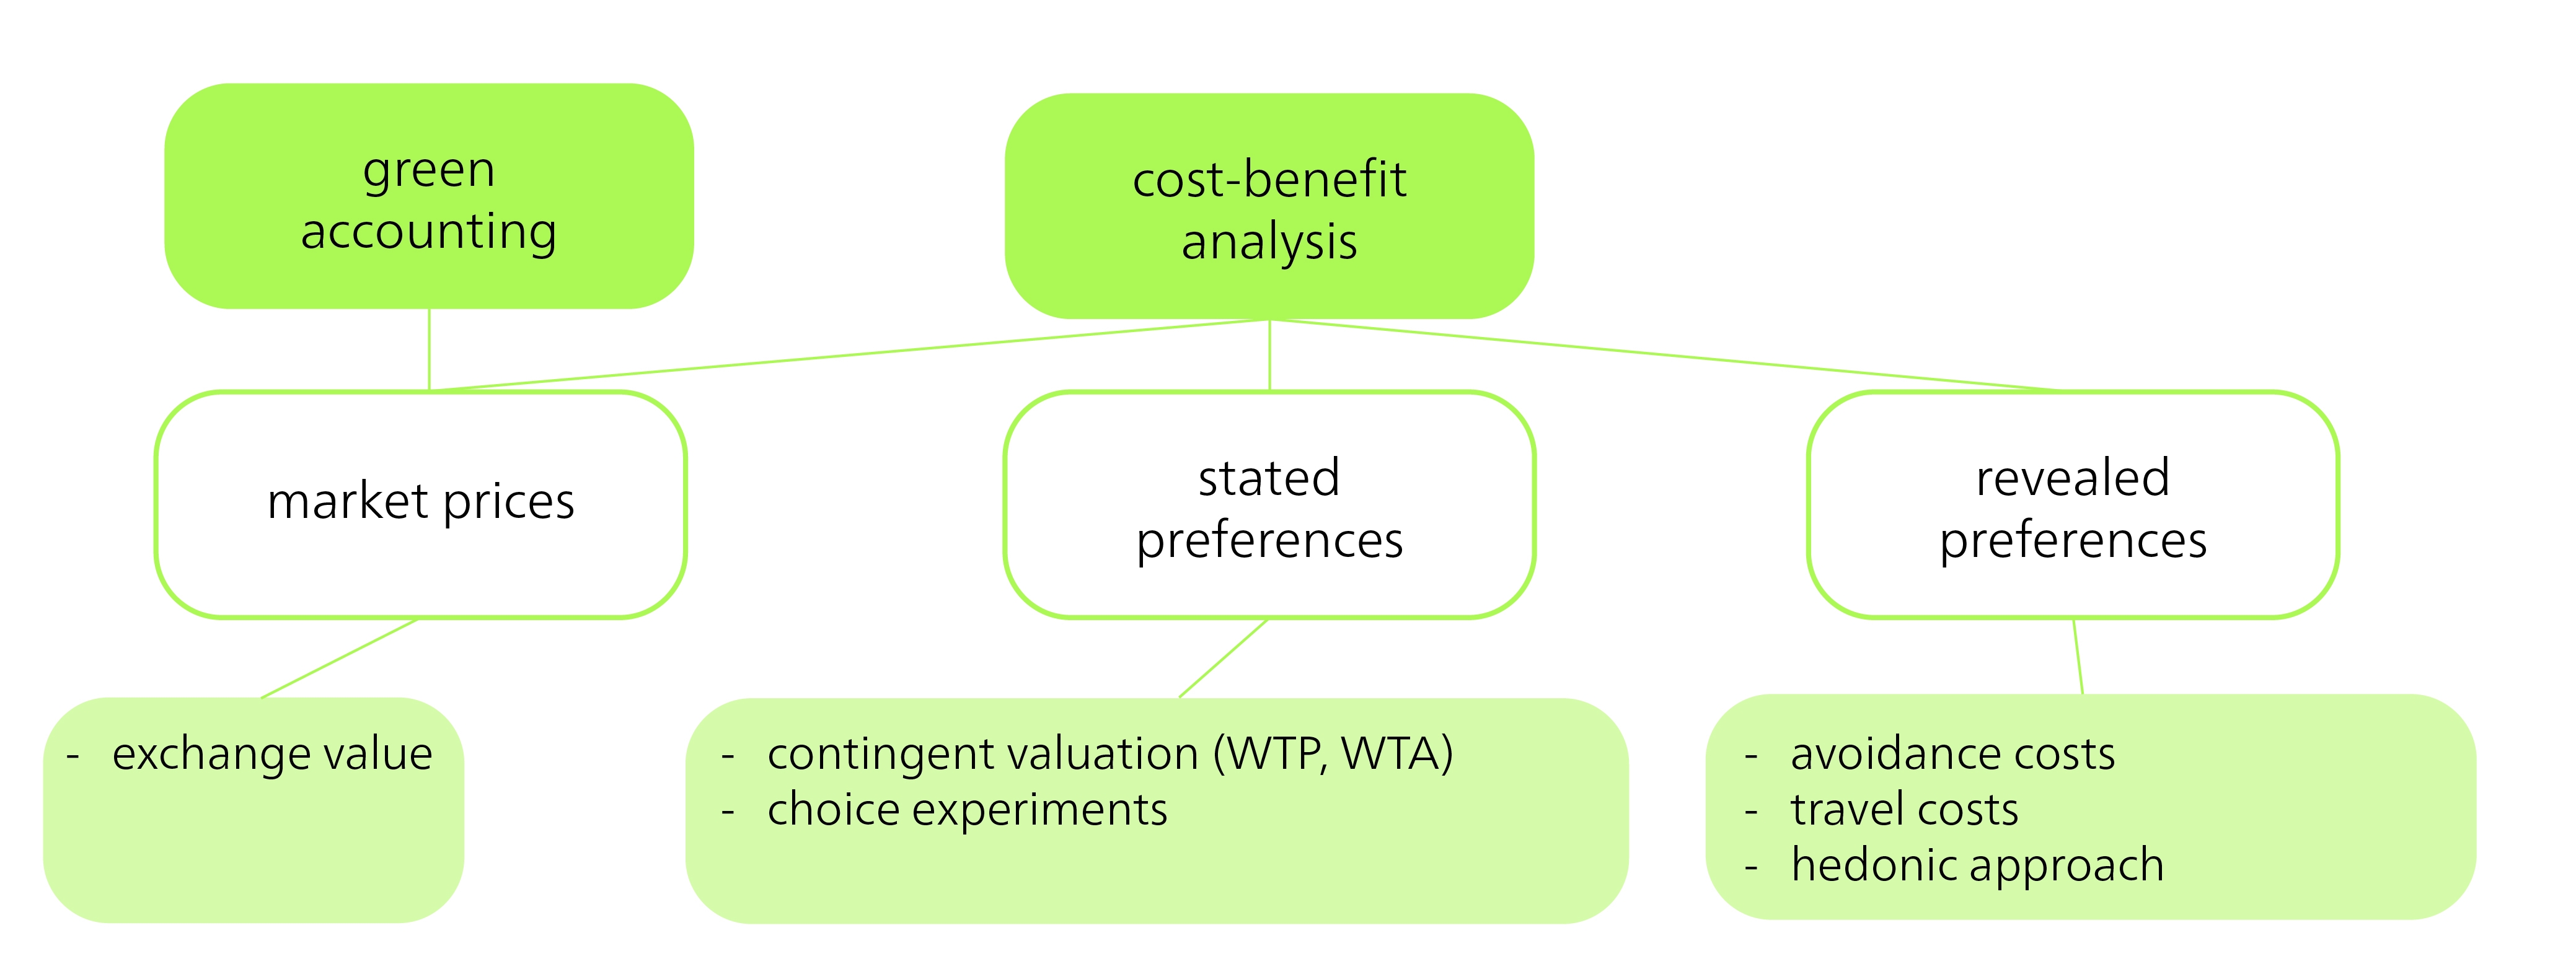
\includegraphics[keepaspectratio]{3_ecological-sustainability/images/Images_en/Fig3_3__EcosystemValuation.jpg}}

}

\caption{\label{fig-monetary-value}the monetary value of ecosystem
services (Quelle?)}

\end{figure}%

\textbf{Stated preferences} involves people stating (e.g.~in a survey)
the extent to which they would be willing to pay for certain ecosystem
services, or which changes they would be willing to accept (contingent
valuation). Another variation of this method involves choosing between
different (usually sub-optimal) options, each representing a trade-off
based on changes in ecosystem services (which are then analysed
econometrically). In contrast, \textbf{revealed preferences} are based
on actual behaviour. For example, it involves analysing avoidance costs
(e.g.~how much people pay for noise barriers) or calculating travel
costs (which assumes that the time and travel costs incurred for
visiting a destination reflect the value of the place, and thus, in a
broader sense, an ecosystem service). Other methods include using
hedonic approaches to determine the extent to which favourable or
unfavourable environmental influences, and thus their quality, can
affect the value of a property.

Each of these methods has its advantages and disadvantages. They are
criticized mainly for their one-sided assessments and failure to account
for social inequalities, power relations, and cultural differences.
Consequently, these methods are limited in their ability to promote fair
and environmentally sustainable decisions (see next chapter).

The principle behind \textbf{Payments for Ecosystem Services (PES)}
involves compensating land users for maintaining a component of a
specific ecosystem service. Such compensation may, for example, be paid
by organizations or companies for which these specific ecosystem
services are important. A well-known example of PES is the ``Pagos por
Servicios Ambientales'' (PSA) programme in Costa Rica. This national
programme, which has been operational since 1997, was set up to reduce
deforestation and promote reforestation by paying landowners to
maintain, reforest, or sustainably manage forest areas. The payments aim
to promote the provision of ecosystem services such as carbon
sequestration, water conservation, biodiversity conservation, and scenic
beauty. The payments in this project come from various sources,
including a tax on fuels and international funding from organizations
interested in carbon offsetting. Studies show that the programme has
significantly reduced the rate of deforestation in the country and
promoted the conservation of biodiversity, while at the same time
increasing the income of landowners (Quelle: Porras et al.~2013).

\section{Criticism of ecosystem services, and further and alternative
concepts}\label{criticism-of-ecosystem-services-and-further-and-alternative-concepts}

While the concept of ecosystem services has been recognized and applied
in the scientific and policy debate, it has also been widely criticized
(Quellen: see e.g.~Norgaard, 2010; Kosoy \& Corbera, 2010). One argument
is that by focusing on ecosystem services, we reduce the complex and
diverse values of ecosystems to their monetary benefits for humans
(Quelle: cf.~Schröter et al.~2014). This \textbf{economic reduction of
nature} neglects the non-quantifiable but nevertheless important aspects
of nature, such as spiritual or intrinsic values (Quelle: Fairhead er
al.~2012). The commodification of nature through ecosystem services
could ultimately also lead to an exploitative relationship between
humans and nature (cf.~Schröter et al.~2014) or \textbf{an exacerbation
of social inequalities between powerful actors and marginalized groups}
(Quelle: Dawson et al.~2021), as the concept does not explicitly
consider justice (Quelle: Loos et al.~2023: 478). In some cases, it is
even assumed that the concept of ecosystem services could conflict with
-- and undermine -- biodiversity conservation (cf.~Schröter et
al.~2014).

\begin{quote}
``The flurry of enthusiasm for optimizing the economy by including
ecosystem services has blinded us to the more important question of how
we are going to make the substantial institutional changes to
significantly reduce human pressure on ecosystems, especially by the
rich, and to adapt to and work effectively with the rapid ecosystem
changes being driven by existing and foreseeable climate dynamics.''

--- Norgaard 2010: 1220
\end{quote}

In response to this criticism, the IPBES (Intergovernmental Platform on
Biodiversity and Ecosystem Services), (see Biodiversity chapter) has
further developed the concept of ecosystem services and developed
another concept, that of \emph{Nature's Contribution to People} (NCP).
NCPs are defined as ``all the positive contributions, or benefits,
\emph{and} occasionally negative contributions, losses or detriments,
that people obtain from nature.'' (Quelle: Pascual et al.~2017: 9). The
concept may resemble ecosystem services, but it goes further and
recognizes that nature and its contributions to a good life can be
perceived and viewed in different ways, depending on the cultural and
institutional context. The concept seeks to include different world
views, such as Indigenous knowledge systems, thus taking into account
both intrinsic (i.e.~non-anthropocentric) and relational values of
nature (Quelle: Díaz et al.~2018). Overall, this approach also includes
context-specific perspectives, and it gives greater consideration to the
justice dimensions than the concept of ecosystem services does (Quelle:
Loos et al.~2023).

However, such \textbf{plural valuations} are also subject to criticism
and pose various challenges. For example, Jacobs et al.~(2023) point out
that current approaches to integrating multiple values and perspectives
into ecosystem assessments risk merely promoting pseudo-participation,
while existing \textbf{structures of power and discrimination} remain
unchanged. Plural valuations aim for inclusivity and democracy, but they
can inadvertently lead to conflict, power imbalances, and unclear
outcomes if not carefully designed. Scientists have also criticized the
above-mentioned NCP concept, which is often seen as an inadequate
development of \textbf{utilitarian environmentalism}. This is a strongly
Western and anthropocentric perspective that maintains a dualistic
separation of humans and nature (Quelle: cf.~Muradian \&
Gomez-Baggethun, 2021). Muradian \& Gomez-Baggethun (2021: 7), propose
that ``in order to induce transformative change in human-nature
relations we need a shift from a morality of utility to a morality of
care, a reallocation of property rights, and the extension of the
community of justice to non-human entities.'' A notable example of this
transformation is the 2017 recognition of New Zealand's Whanganui River
as a legal person (Quelle: see Charpleix, 2018).

\section{Planetary boundaries}\label{planetary-boundaries}

The current era is called the Anthropocene because human activities are
exerting an increasingly profound impact on the Earth and its systems.
Although this term has not (yet) been recognized as an official geologic
or geochronological epoch by geological bodies (Quelle:
\href{https://www.nytimes.com/2024/03/05/climate/anthropocene-epoch-vote-rejected.html?unlocked_article_code=1.aU0.b2Ag.EdNlTI4oneVq&smid=url-share}{link}),
it is used to describe the enormous human impact on the environment.
There is no uniform definition of the origins of the Anthropocene;
possible markers include human impact on greenhouse gas concentrations
through rice cultivation, the global spread of radioactivity from
nuclear testing, or the appearance of plastic particles in geological
sediments. The Industrial Revolution is generally considered the start
of the Anthropocene.

A quantitative definition of environmental sustainability was proposed
by Rockström et al.~(2009) and Steffen et al.~(2015), who identified
nine planetary boundaries: climate change, biosphere integrity,
land-system change, freshwater change, biogeochemical flows, ocean
acidification, atmospheric aerosol loading, stratospheric ozone
depletion, and novel entities. These planetary boundaries serve as a
scientific reference point and show the limits within which our global
socio-economic systems must operate to ensure the well-being of humanity
(see also the Debates section).

This chapter focuses on three of these boundaries, described here as
\textbf{climate change}, \textbf{land use change}, and
\textbf{biodiversity loss}. These three crises are mutually reinforcing
and form a complex web of interactions.

\begin{figure}[H]

\centering{

\pandocbounded{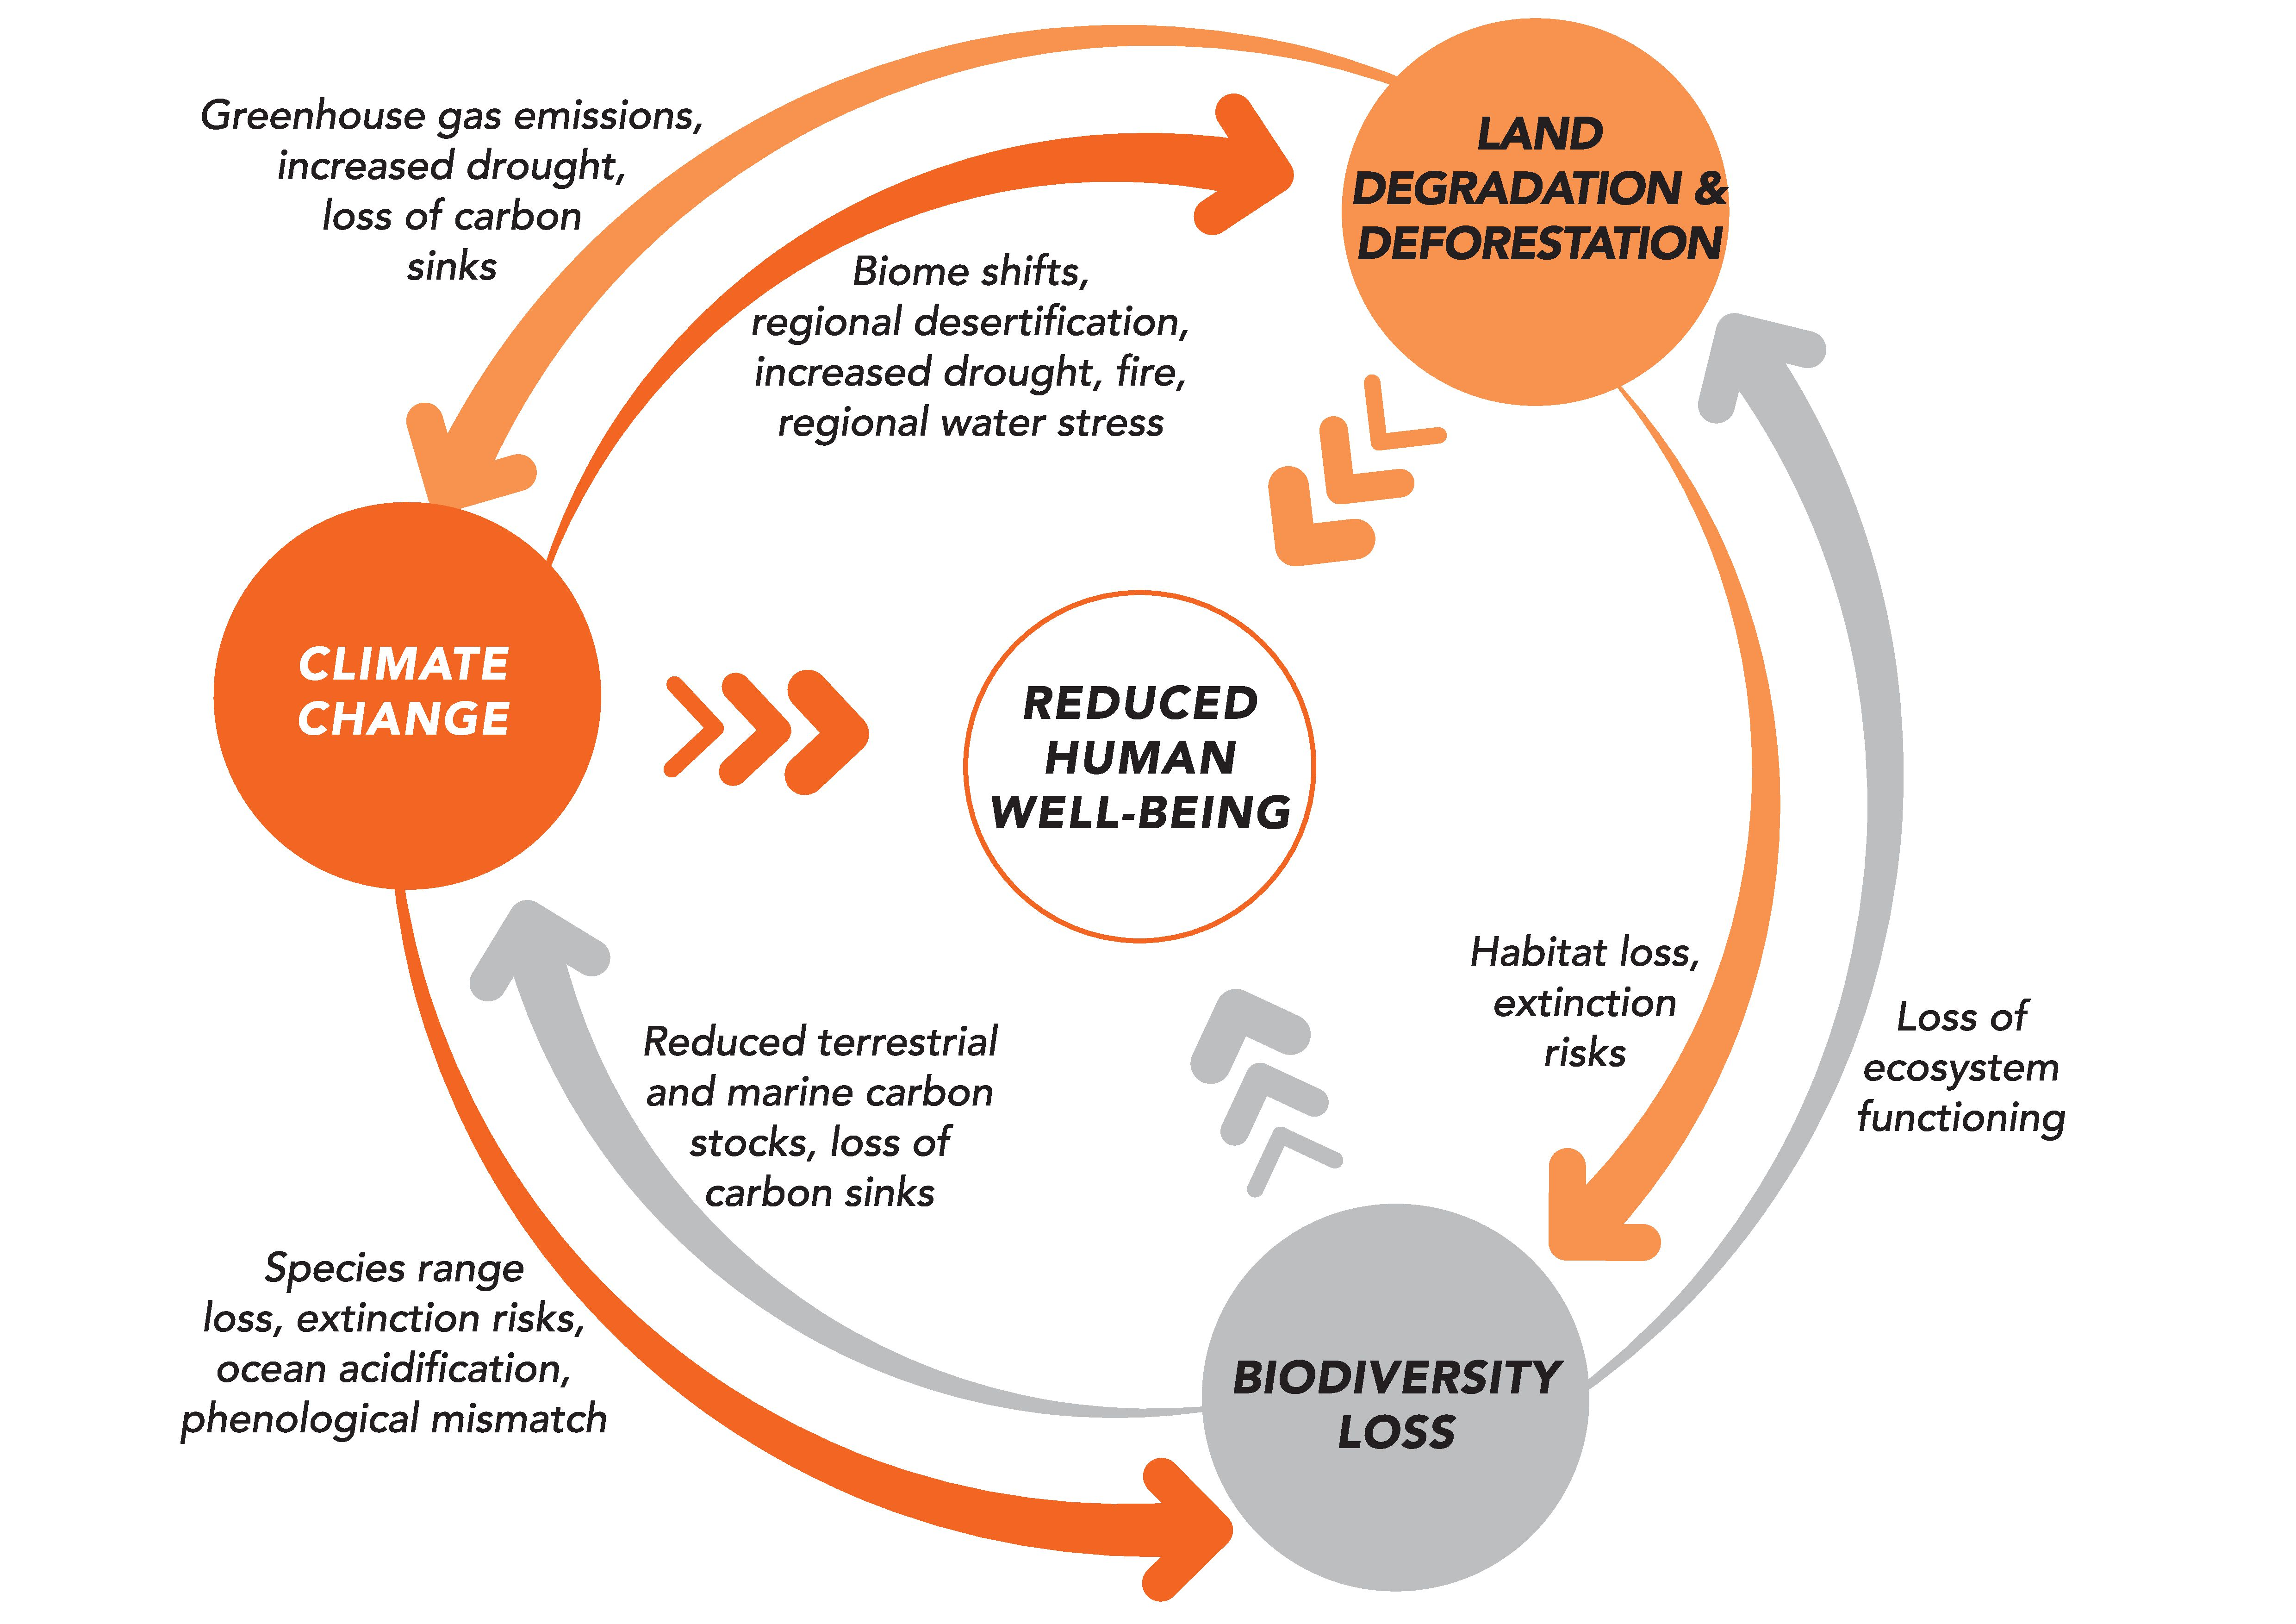
\includegraphics[keepaspectratio]{3_ecological-sustainability/images/Land-Climate-Biodiversity (UNEP 2021).jpg}}

}

\caption{\label{fig-interactions}Interactions between biodiversity,
climate change and land use (Source: UNEP (2021b))}

\end{figure}%

\subsection{The climate crisis (climate
change)}\label{the-climate-crisis-climate-change}

\textbf{Climate change} -- or, to use a term more illustrative of the
urgency, the climate crisis -- is one of the most pressing issues of our
time. It receives much media attention and is exemplary of a ``wicked''
problem (see page 13; Hulme, 2009). It is the focus of the Fridays for
Future movement that was initiated by Greta Thunberg, and it is a topic,
of discussion at least, on the (global) political stage. While local
conditions and natural fluctuations contribute to some uncertainties in
climate models and statistics, the scientific evidence clearly shows
that rising global temperatures have an enormous impact on environmental
sustainability and human well-being. This is why climate change is one
of the nine planetary boundaries.

The term \textbf{climate} describes the average state of the atmosphere
(temperature, precipitation, humidity, etc.) over a period of at least
30 years at a specific location. By contrast, \textbf{weather} describes
the short-term state (i.e.~from seconds to weeks) and includes weather
phenomena such as thunderstorms or heat waves (source - NCCS.admin). The
\textbf{climate system}, in turn, encompasses not only the atmosphere
but also the hydrosphere (oceans, lakes, rivers, groundwater), the
cryosphere (glaciers, snow cover, sea and lake ice, permafrost), the
biosphere (living organisms), and the lithosphere (soils or the
outermost layer of the earth). In particular, it refers to the physical,
biological, and chemical interactions and interdependencies between
these five spheres. In addition, the climate system is influenced by
radiation from space (see figure below).

Figure?

Material and energy flows between the various components of the climate
system, such as the carbon cycle, can act as \textbf{feedback
mechanisms}. We have already learnt about such feedback mechanisms in
the chapter on systemic effects (see p.~XX). These can either be
positive, if the feedback reinforces the original change, or negative,
if the feedback attempts to reverse the original change. Here are
examples of a positive and negative feedback effect in the climate
system:

\begin{itemize}
\item
  \textbf{Positive feedback}: When the Earth's surface temperature
  increases, so does water evaporation, creating a positive feedback
  loop. Water vapour is the most significant \textbf{greenhouse gas} in
  the atmosphere. As temperatures rise, more water vapour enters the
  atmosphere, increasing the reflection of heat back to the Earth's
  surface and leading to further evaporation. This cycle accelerates
  warming and atmospheric water vapour accumulation. On Venus, this
  feedback mechanism intensified the greenhouse effect to the point
  where all liquid surface water evaporated.
\item
  \textbf{Negative feedback}: Increased atmospheric CO\textsubscript{2}
  can enhance photosynthesis, a process known as
  \textbf{CO\textsubscript{2} fertilization} and an example of a
  negative feedback mechanism. Although an increase in carbon dioxide
  can cause plants to bind more carbon in biomass than before, it is far
  from sufficient to compensate for the increasing CO\textsubscript{2}
  content in the atmosphere, which is mainly caused by the burning of
  fossil fuels and changes in land use. The ability of plants to take up
  additional CO\textsubscript{2} is limited by various factors such as
  nutrient availability, water resources, and temperature conditions.
  Therefore, this feedback mechanism is insufficient in compensating for
  the increase in atmospheric CO\textsubscript{2} concentrations caused
  by human activities.
\end{itemize}

Positive feedback mechanisms or the failure of negative feedback can
lead to significant \emph{thresholds} being exceeded in the climate
system. These thresholds are referred to as \textbf{tipping points of
the climate system} and are closely linked to the concept of planetary
boundaries (see Debates chapter). When these thresholds are exceeded,
abrupt and often irreversible changes can occur in the climate system,
destabilizing the climate and leading to accelerated climate change. The
concept of tipping points emphasizes the urgency of limiting global
warming and reducing greenhouse gas emissions. Exceeding these
thresholds will make it increasingly difficult to control climate change
or minimize its effects. Ultimately, the Earth risks becoming a large
greenhouse (\emph{Hothouse Earth} scenario) (see
Figure~\ref{fig-hothouse-earth}).

\begin{figure}[H]

\centering{

\pandocbounded{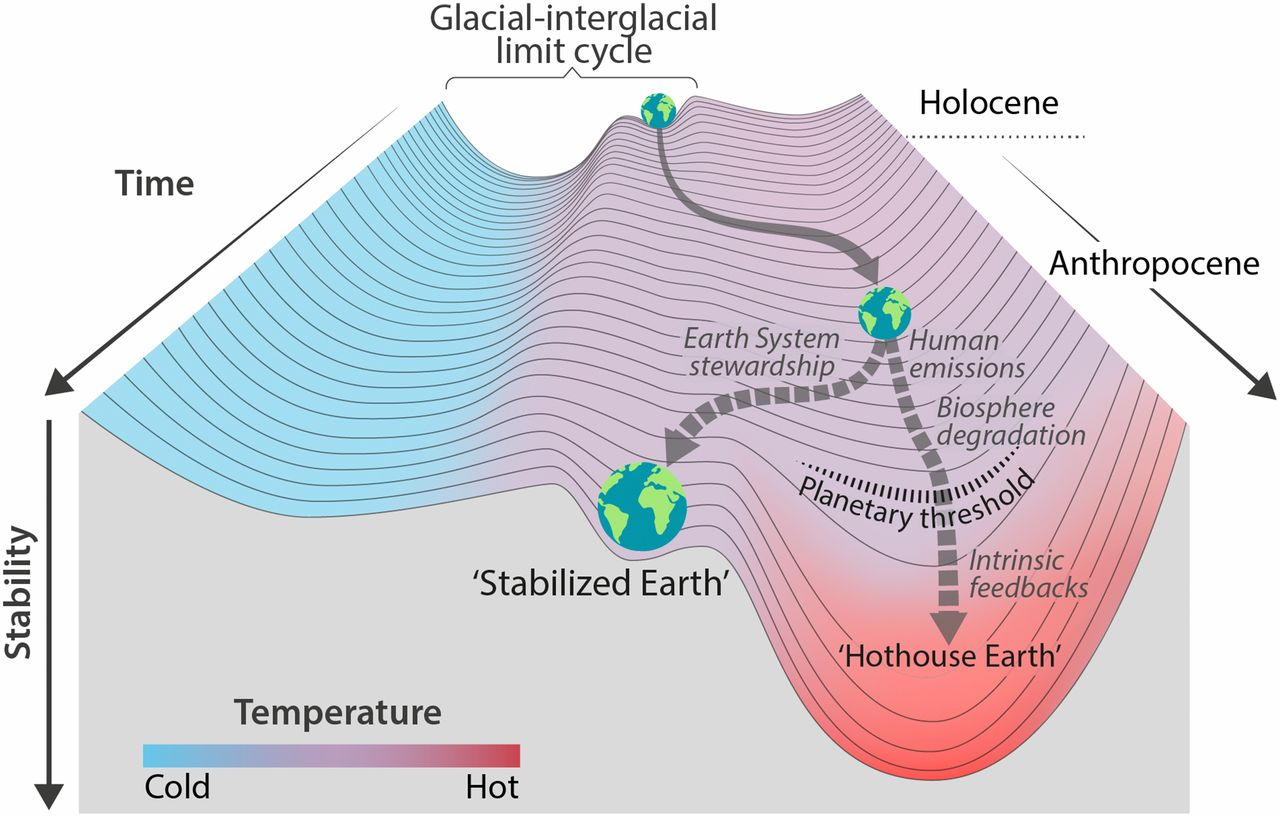
\includegraphics[keepaspectratio]{3_ecological-sustainability/images/Images_en/Fig3_6__HothouseEarth.jpeg}}

}

\caption{\label{fig-hothouse-earth}Hothouse Earth scenario (Source:
Steffen et al.~2018)}

\end{figure}%

A total of 16 tipping points are assumed to exist
(Figure~\ref{fig-16-tipping-points}), including the Siberian permafrost
soils or the West Antarctic Ice Sheet. These tipping points have
different threshold values, meaning that some will be reached earlier,
with less global warming than others. If these tipping points are
reached or exceeded, they can trigger self-reinforcing feedback effects
that lead to further warming, initiate further tipping points, and
intensify climate change. Some of these tipping points are already in a
critical state, as explained impressively by Johan Rockström, one of the
founders of the Planetary Boundaries concept
(\url{https://m.youtube.com/watch?v=Vl6VhCAeEfQ}). In the Amazon, for
example, some areas now emit more CO\textsubscript{2} than they absorb
-- becoming carbon \emph{sources} rather than sinks -- due to forest
fires, climate-change-induced water stress, and deforestation (see Land
use chapter) (Gatti et al.~2021; Harris et al.~2021). Consequently, the
Amazon is already in transition and losing resilience (Flores et
al.~2024). Another worrying and very real tipping point is the
\emph{Atlantic Meridional Overturning Circulation}, or AMOC (Rahmstorf,
2024; \url{https://www.youtube.com/watch?v=ZHNNW8c_FaA}). The AMOC is
nearing its tipping point (van Westen et al.~2024), with projections
suggesting it could collapse as early as the middle of this century
(Ditlevsen \& Ditlevsen, 2023). A collapse would lead to increased
European heat waves and sea-level rise along the north-eastern US coast
(Rahmstorf, 2024).

\begin{figure}[H]

\centering{

\pandocbounded{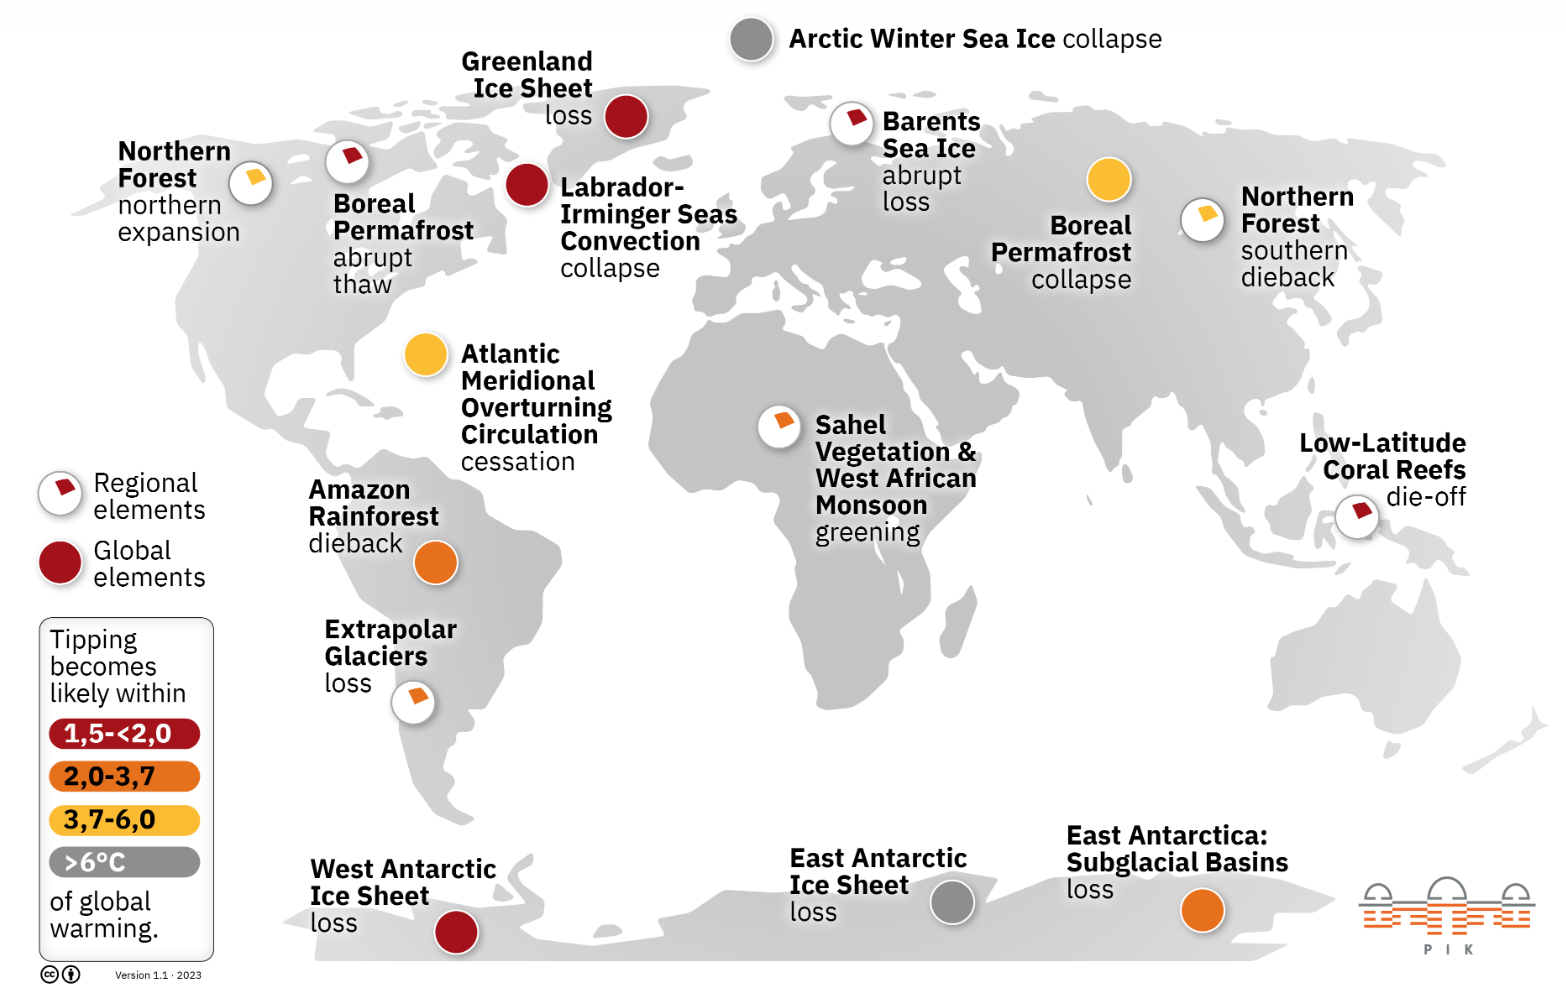
\includegraphics[keepaspectratio]{3_ecological-sustainability/images/Images_en/Fig3_7__tippingpoints.png}}

}

\caption{\label{fig-16-tipping-points}The 16 tipping points and their
likelihood of occurring due to global warming (Quelle: based on
Armstrong McKay et al.~(2022))}

\end{figure}%

But what is causing the Earth to warm and climate change to occur? In
addition to natural causes of climate change such as geological,
long-term causes (Earth's axial rotation, Milanković cycles, volcanic
eruptions), the primary driver of global warming is the
\textbf{greenhouse gas effect}. The greenhouse gas effect is a process
where short-wave solar radiation enters the Earth's atmosphere and is
re-emitted from the Earth's surface as long-wave infrared radiation.
Greenhouse gases -- such as carbon dioxide, methane, and water vapour --
absorb some of this infrared radiation and emit it in all directions,
causing some of the heat to return to the Earth's surface. Without this
effect, the Earth would be too cold to support life. Today, however,
there are too many greenhouse gases in the atmosphere due to
anthropogenic emissions, causing the earth to warm up.

The largest share of human CO\textsubscript{2} emissions, around ¾ of
the global total, originates from energy production, i.e.~primarily
electricity and heat generation
(Figure~\ref{fig-global-greenhouse-gas-emissions}). This is largely due
to the combustion of coal, gas, and oil, with emissions from industry
(comprising 24.2\% of the global total), transport (16.2\%), buildings
(17.5\%), and agriculture (18.4\%). The main drivers of agricultural
emissions are livestock farming, deforestation for agricultural land,
and the use of nitrogen fertilizers on agricultural soils.

Within the transport sector, air traffic accounts for 1.9\% of global
emissions (see figure below). In Switzerland, however, flights account
for about 11\% of national emissions. These flight emissions are largely
attributable to international air traffic (FOEN, 2025), although the
calculations exclude Basel-Mulhouse Airport, which is located on French
soil. Despite this evidence, Switzerland has not yet introduced a
CO\textsubscript{2} tax on kerosene (the main component of aviation
fuel), although there is one on fossil fuels such as heating oil and
natural gas. It should however be noted that climate impact is not
solely determined by greenhouse gas emissions (Allen et al., 2018; Lee
et al., 2021; Neu, 2021). The warming potential of air travel can thus
be significantly higher than indicated by greenhouse gas emissions
alone, as non-CO\textsubscript{2} effects from flights -- such as water
vapour, nitrogen oxides (NOx), and soot -- also affect the climate (Lee
et al., 2021).

Globally, air travel emissions have more than doubled since 1990, driven
primarily by international flights. Despite a sharp drop in the number
of flights in 2020 due to the pandemic, flight emissions have rebounded
and are projected to surpass 2019's record levels in the coming years.
(Aviation emissions worldwide - statistics \& facts \textbar{}
Statista{]}(https://www.statista.com/topics/12910/aviation-emissions-worldwide/\#topicOverview)

\begin{figure}[H]

\centering{

\pandocbounded{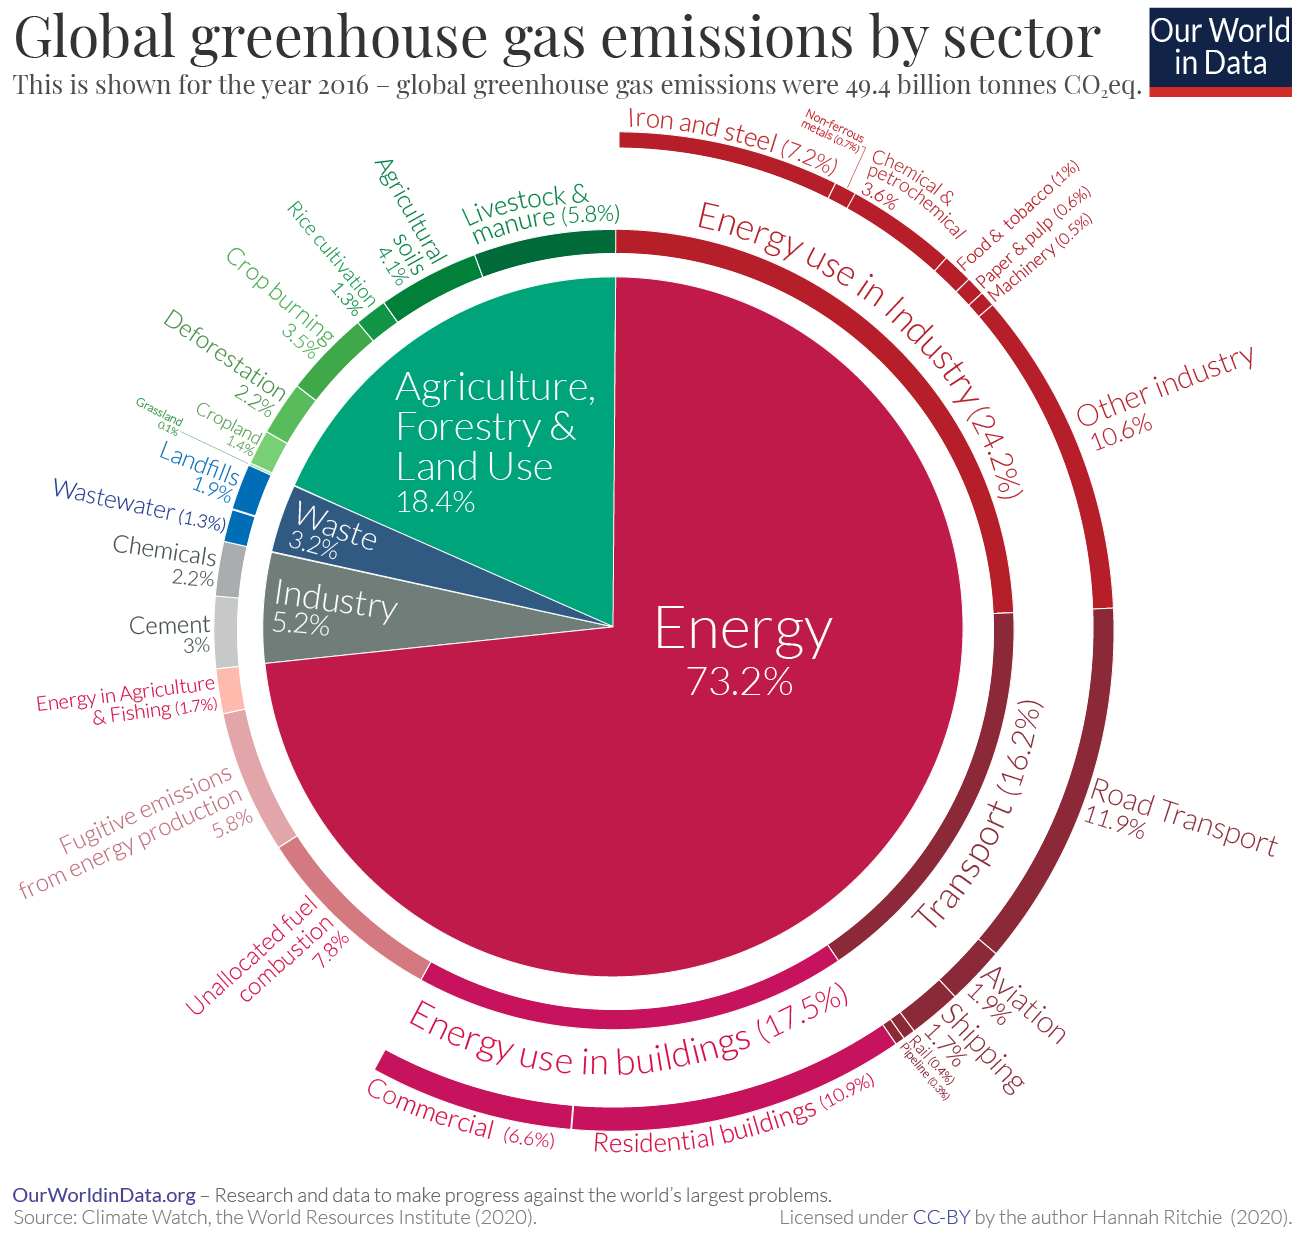
\includegraphics[keepaspectratio]{3_ecological-sustainability/images/Images_en/Fig3_8__GreenhouseSector.png}}

}

\caption{\label{fig-global-greenhouse-gas-emissions}Global greenhouse
gas emissions by sector (Source: Climate Watch, the World Resources
Institute (2020))}

\end{figure}%

Recent calculations and climate reports indicate that the Earth's
temperature has risen by around 1.2°C in the last 10 years (2014--2023)
compared to pre-industrial levels (1850--1900). In addition, 2023 was
the warmest year on record, with a global surface temperature of 1.45°C
above the pre-industrial baseline. This may not sound like much, but it
represents a substantial heat increase, given the oceans' vast size and
heat storage capacity.
(https://www.un.org/sites/un2.un.org/files/temperaturerise\_may2024.pdf)
(https://ourworldindata.org/ghg-emissions-by-sector)

\begin{figure}[H]

\centering{

\pandocbounded{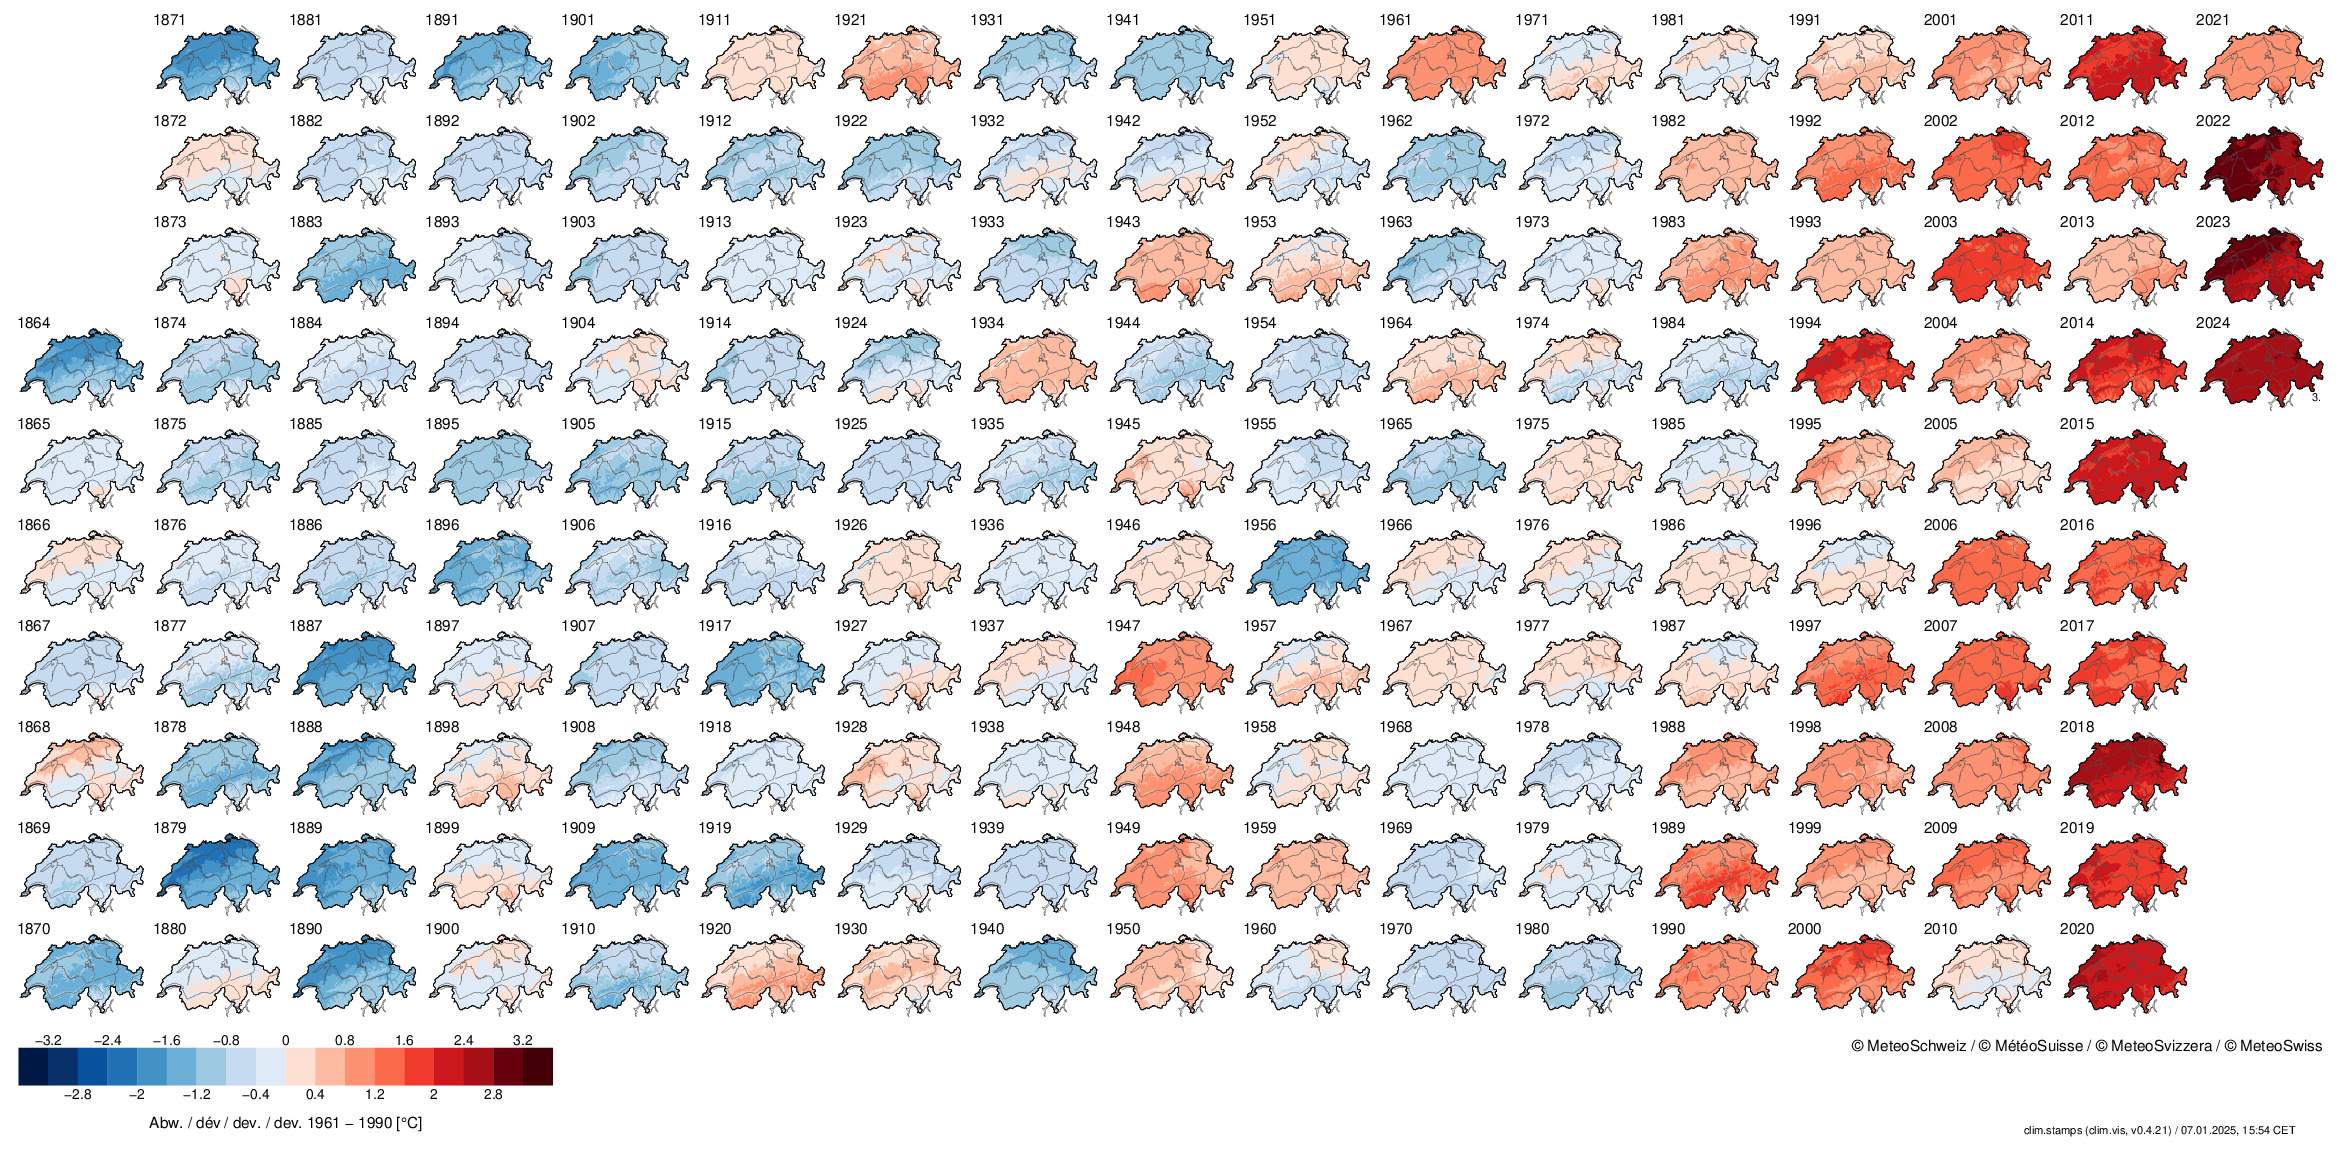
\includegraphics[keepaspectratio]{3_ecological-sustainability/images/Images_en/Fig3_9__KlimaCH.jpg}}

}

\caption{\label{fig-worlds}What is climate (Slurce:
https://www.nccs.admin.ch/nccs/en/home/climate-change-and-impacts/climate-basics/what-is-climate-.html)}

\end{figure}%

\begin{figure}[H]

\centering{

\pandocbounded{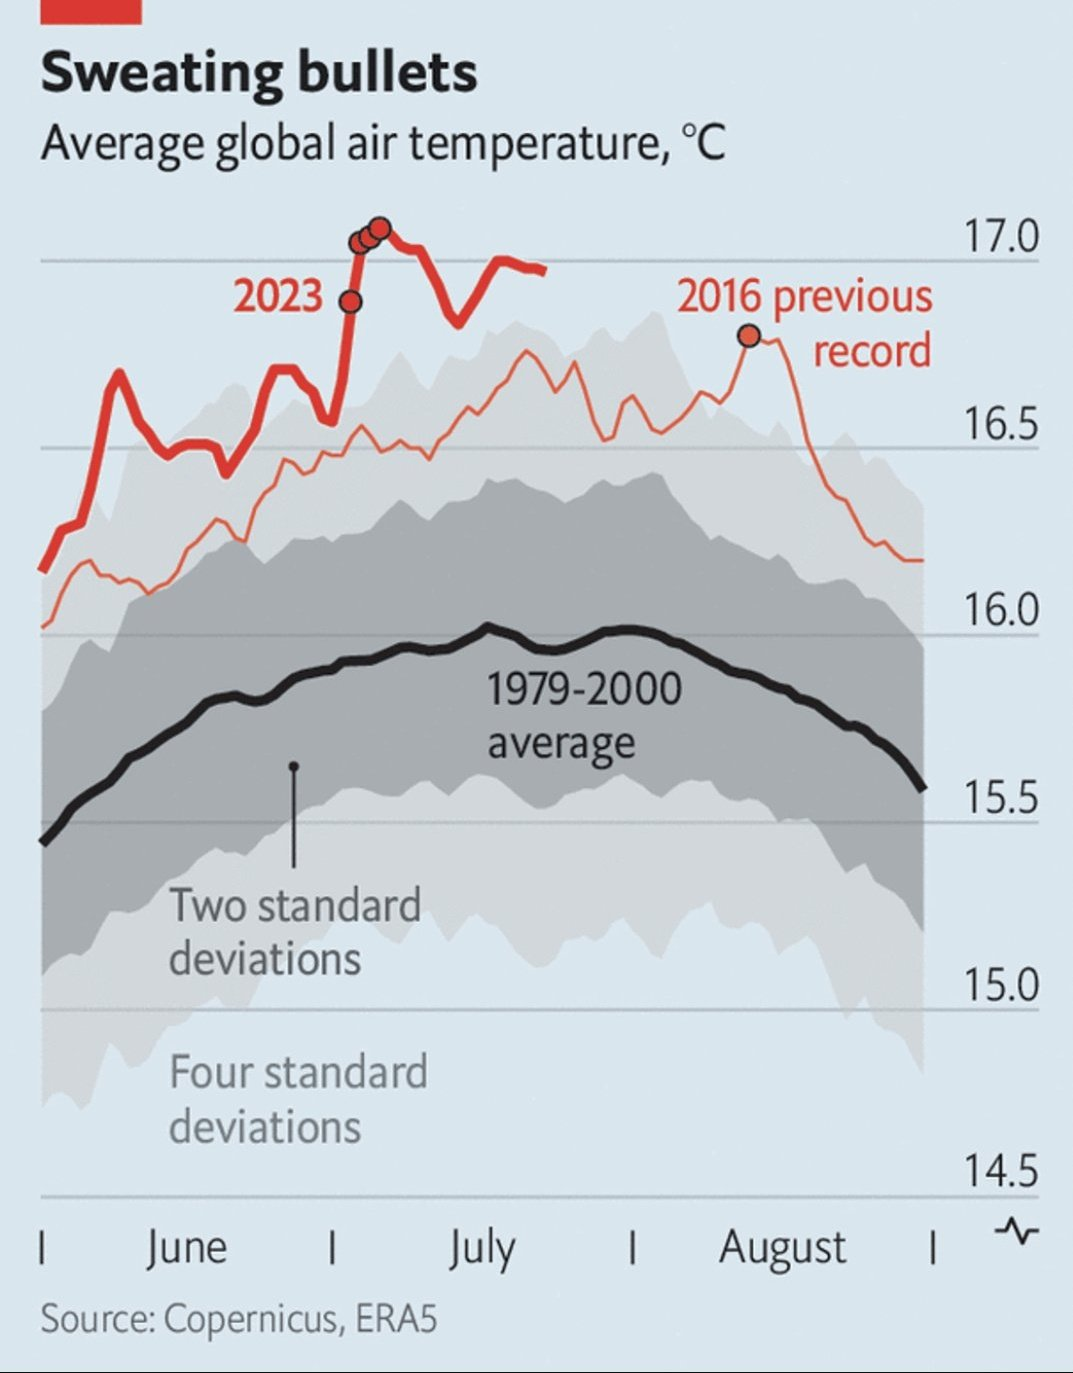
\includegraphics[keepaspectratio]{3_ecological-sustainability/images/Sweating Bullets (X - Economist).jpg}}

}

\caption{\label{fig-sweating-bullets}Sweating bullets (Source:
https://twitter.com/i/status/1685941280151379969)}

\end{figure}%

The \textbf{Paris Climate Agreement}, adopted in December 2015, was the
first international treaty where industrialized and emerging countries
jointly pledged to curb greenhouse gas emissions. Its core objective is
to limit global temperature rise to a maximum of 2°C, with efforts to
pursue a 1.5°C limit, relative to pre-industrial times. In 2018, the
Intergovernmental Panel on Climate Change (IPCC, see box) published a
Special Report containing some startling facts: Most notably, that we
only have few years left -- until 2030 -- to avoid exceeding 2°C. The
next major decision in international efforts that built on the Paris
Climate Agreement was the 2022 climate conference, COP 27. At COP 27,
signatories agreed to establish the Loss and Damage Fund, a result of
decades of prior discussion, designed to help developing countries to
receive financial support after extreme weather events.

\begin{tcolorbox}[enhanced jigsaw, left=2mm, arc=.35mm, titlerule=0mm, opacityback=0, leftrule=.75mm, title={Note}, breakable, bottomtitle=1mm, rightrule=.15mm, coltitle=black, toptitle=1mm, bottomrule=.15mm, colback=white, opacitybacktitle=0.6, colbacktitle=quarto-callout-note-color!10!white, toprule=.15mm, colframe=quarto-callout-note-color-frame]

The \textbf{Intergovernmental Panel on Climate Change (IPCC)},
established in 1988 by the United Nations and the World Meteorological
Organization, synthesizes scientific research on climate change for
policymakers worldwide. Its periodic IPCC reports provide a
comprehensive assessment of the current state of knowledge on climate
change, including the physical foundations, impacts, risks, and
adaptation strategies. These reports are based on thousands of studies
and are recognized as the most authoritative source of information on
climate change. The IPCC reports serve as the basis for international
negotiations and national climate policies, including the Paris
Agreement of 2015.

\end{tcolorbox}

\begin{figure}[H]

\centering{

\pandocbounded{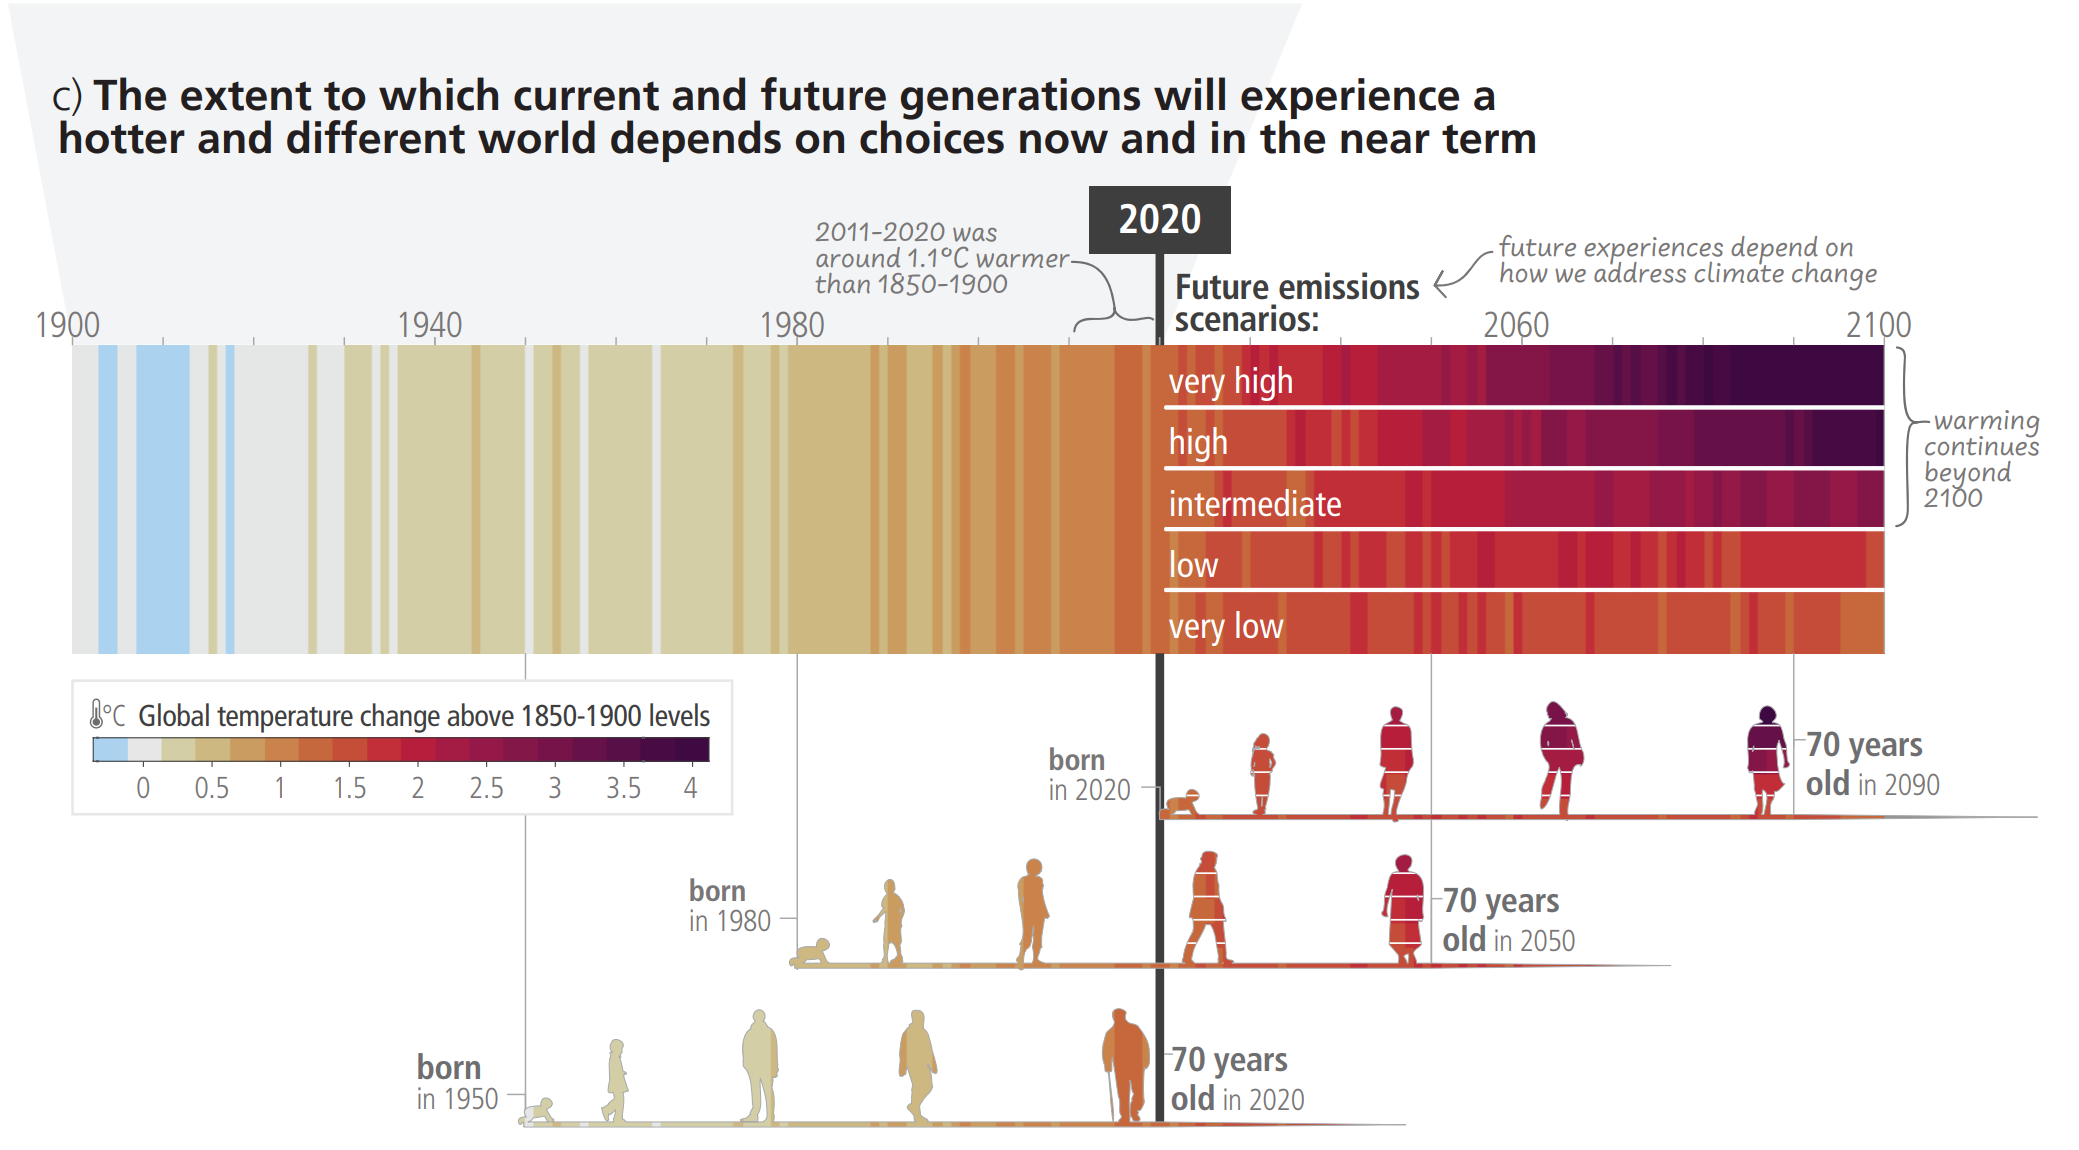
\includegraphics[keepaspectratio]{3_ecological-sustainability/images/Experiencing Climate Change (IPCC AR6).png}}

}

\caption{\label{fig-hotter-and-different-world}Hotter and different
world (Quelle?)}

\end{figure}%

But what will it take to prevent the temperature from rising by more
than 1.5 degrees? A whole lot. Anthropogenic CO\textsubscript{2}
emissions must fall by 45\% between 2010 and 2030, and net
CO\textsubscript{2} emissions must fall to zero by 2050. While we are
adopting greener technologies for marginal activities like car purchases
or building efficiency, we still risk neglecting the serious threat
posed by the carbon that is already in the atmosphere. It's important to
distinguish between ongoing emissions (flow) and accumulated atmospheric
carbon (stock). Flow plays a subordinate role for the planet -- it's the
stock that drives global warming. Climate change is therefore primarily
a stock problem, rather than a flow problem. This is a challenging
concept, not only for laypeople. Indeed, Sterman \& Sweeney (2007)
observed that most adults had difficulty in grasping the stock aspect of
climate change.

Figure - nicht abgespeichert

An effective mental model is the bathtub analogy: if the inflow of water
through the tap (i.e.~our emissions, or flow) exceeds the outflow of
water through the drain (carbon absorption by rainforests, oceans,
etc.), the water level (the atmospheric carbon stock) increases. The
past five years, and twenty of the last twenty-two, have been the
warmest on record. This warming trend is a direct result of the rising
water level in that ``bathtub''. \url{https://youtu.be/jWFxoAhic1o}

\textbf{Impacts}: Climate change is expected to have a range of direct
and indirect impacts, some of which are already occurring. These include
sea level rise, shrinking glaciers, threats to water and food security,
an increase in extreme weather events, adverse health effects related to
temperature, heatwaves, droughts and excessive precipitation, wildfires,
and an increase in geomorphological activities and thus natural hazards
due to permafrost thaw.
\href{https://interactive.carbonbrief.org/impacts-climate-change-one-point-five-degrees-two-degrees/}{Interactive
website: The impacts of climate change at 1.5C, 2C and beyond \textbar{}
Carbon Brief}

\subsection{Land use change}\label{land-use-change}

Land use change, like deforestation for agriculture or urban expansion,
has a significant impact on the \textbf{environmental dimension of
sustainability}. Land use change threatens biodiversity and disrupts
ecosystem functions. It can also increase greenhouse gas emissions,
alter water cycles, or deplete valuable agricultural land. This can
result in a reduction of ecosystem services (see chapter on ecosystem
services), ultimately restricting human well-being. Land use change is
one of the nine \textbf{planetary boundaries} that has already been
exceeded, according to Richardson et al.~(2023).

Some key definitions are needed to understand land use change:

\begin{itemize}
\item
  \textbf{Land cover} refers to the characteristics of the land surface
  and its immediate subsurface, including biota, topography, and human
  structures (Lambin et al.~2000: 322).
\item
  \textbf{Land use} is the way in which humans use land cover (Lambin et
  al.~2000: 322).
\item
  \textbf{Land use change} represents the change from one land use to
  another(Lambin et al.~2000: 322).
\item
  \textbf{Land degradation} means ``reduction or loss, in arid,
  semi-arid and dry sub-humid areas, of the biological or economic
  productivity and complexity of rainfed cropland, irrigated cropland,
  or range, pasture, forest and woodlands resulting from land uses''
  (UNCCD, 1994: 4).
\item
  \textbf{Land systems} ``represent the terrestrial component of the
  Earth system and encompass all processes and activities related to the
  human use of land, including socioeconomic, technological and
  organizational investments and arrangements, as well as the benefits
  gained from land and the unintended social and ecological outcomes of
  societal activities'' (Verburg et al.~2013: 433).
\item
  Land can also be understood as a \textbf{socio-ecological system}
  (Chapin et al.~2006) in which the social and ecological subsystems
  interact and depend on each other. This system is characterized by
  mutual feedback, with humans considered integral components of
  nature(Verburg et al.~2015).
\end{itemize}

Various \textbf{drivers}, i.e.~reasons or causes, are responsible for
the occurrence of land use change. These factors vary depending on the
type of land use. For example, the main drivers of global deforestation,
a form of land use change, are commercial agriculture, slash-and-burn
agriculture, commercial forestry, urbanization, and forest fires (Curtis
et al.~2018). Deforestation has already led to an alarming decline in
biodiversity (see next chapter) and the disruption of carbon cycles (see
previous chapter or box). For example, the Agriculture, Forestry, and
Other Land Use (AFOLU) sector is a major contributor to \textbf{global
anthropogenic greenhouse gas} \textbf{emissions}, accounting for
approximately 13\% of CO\textsubscript{2}, 44\% of CH\textsubscript{4},
and 81\% of N\textsubscript{2}O emissions (IPCC, 2019). These
interactions between climate change and land use/land use change show
that land systems and climate systems should be considered systemically,
rather than in isolation (Richardson et al.~2023). Figure X is a
schematic representation of these interactions between land and
greenhouse gases.

\begin{figure}[H]

\centering{

\pandocbounded{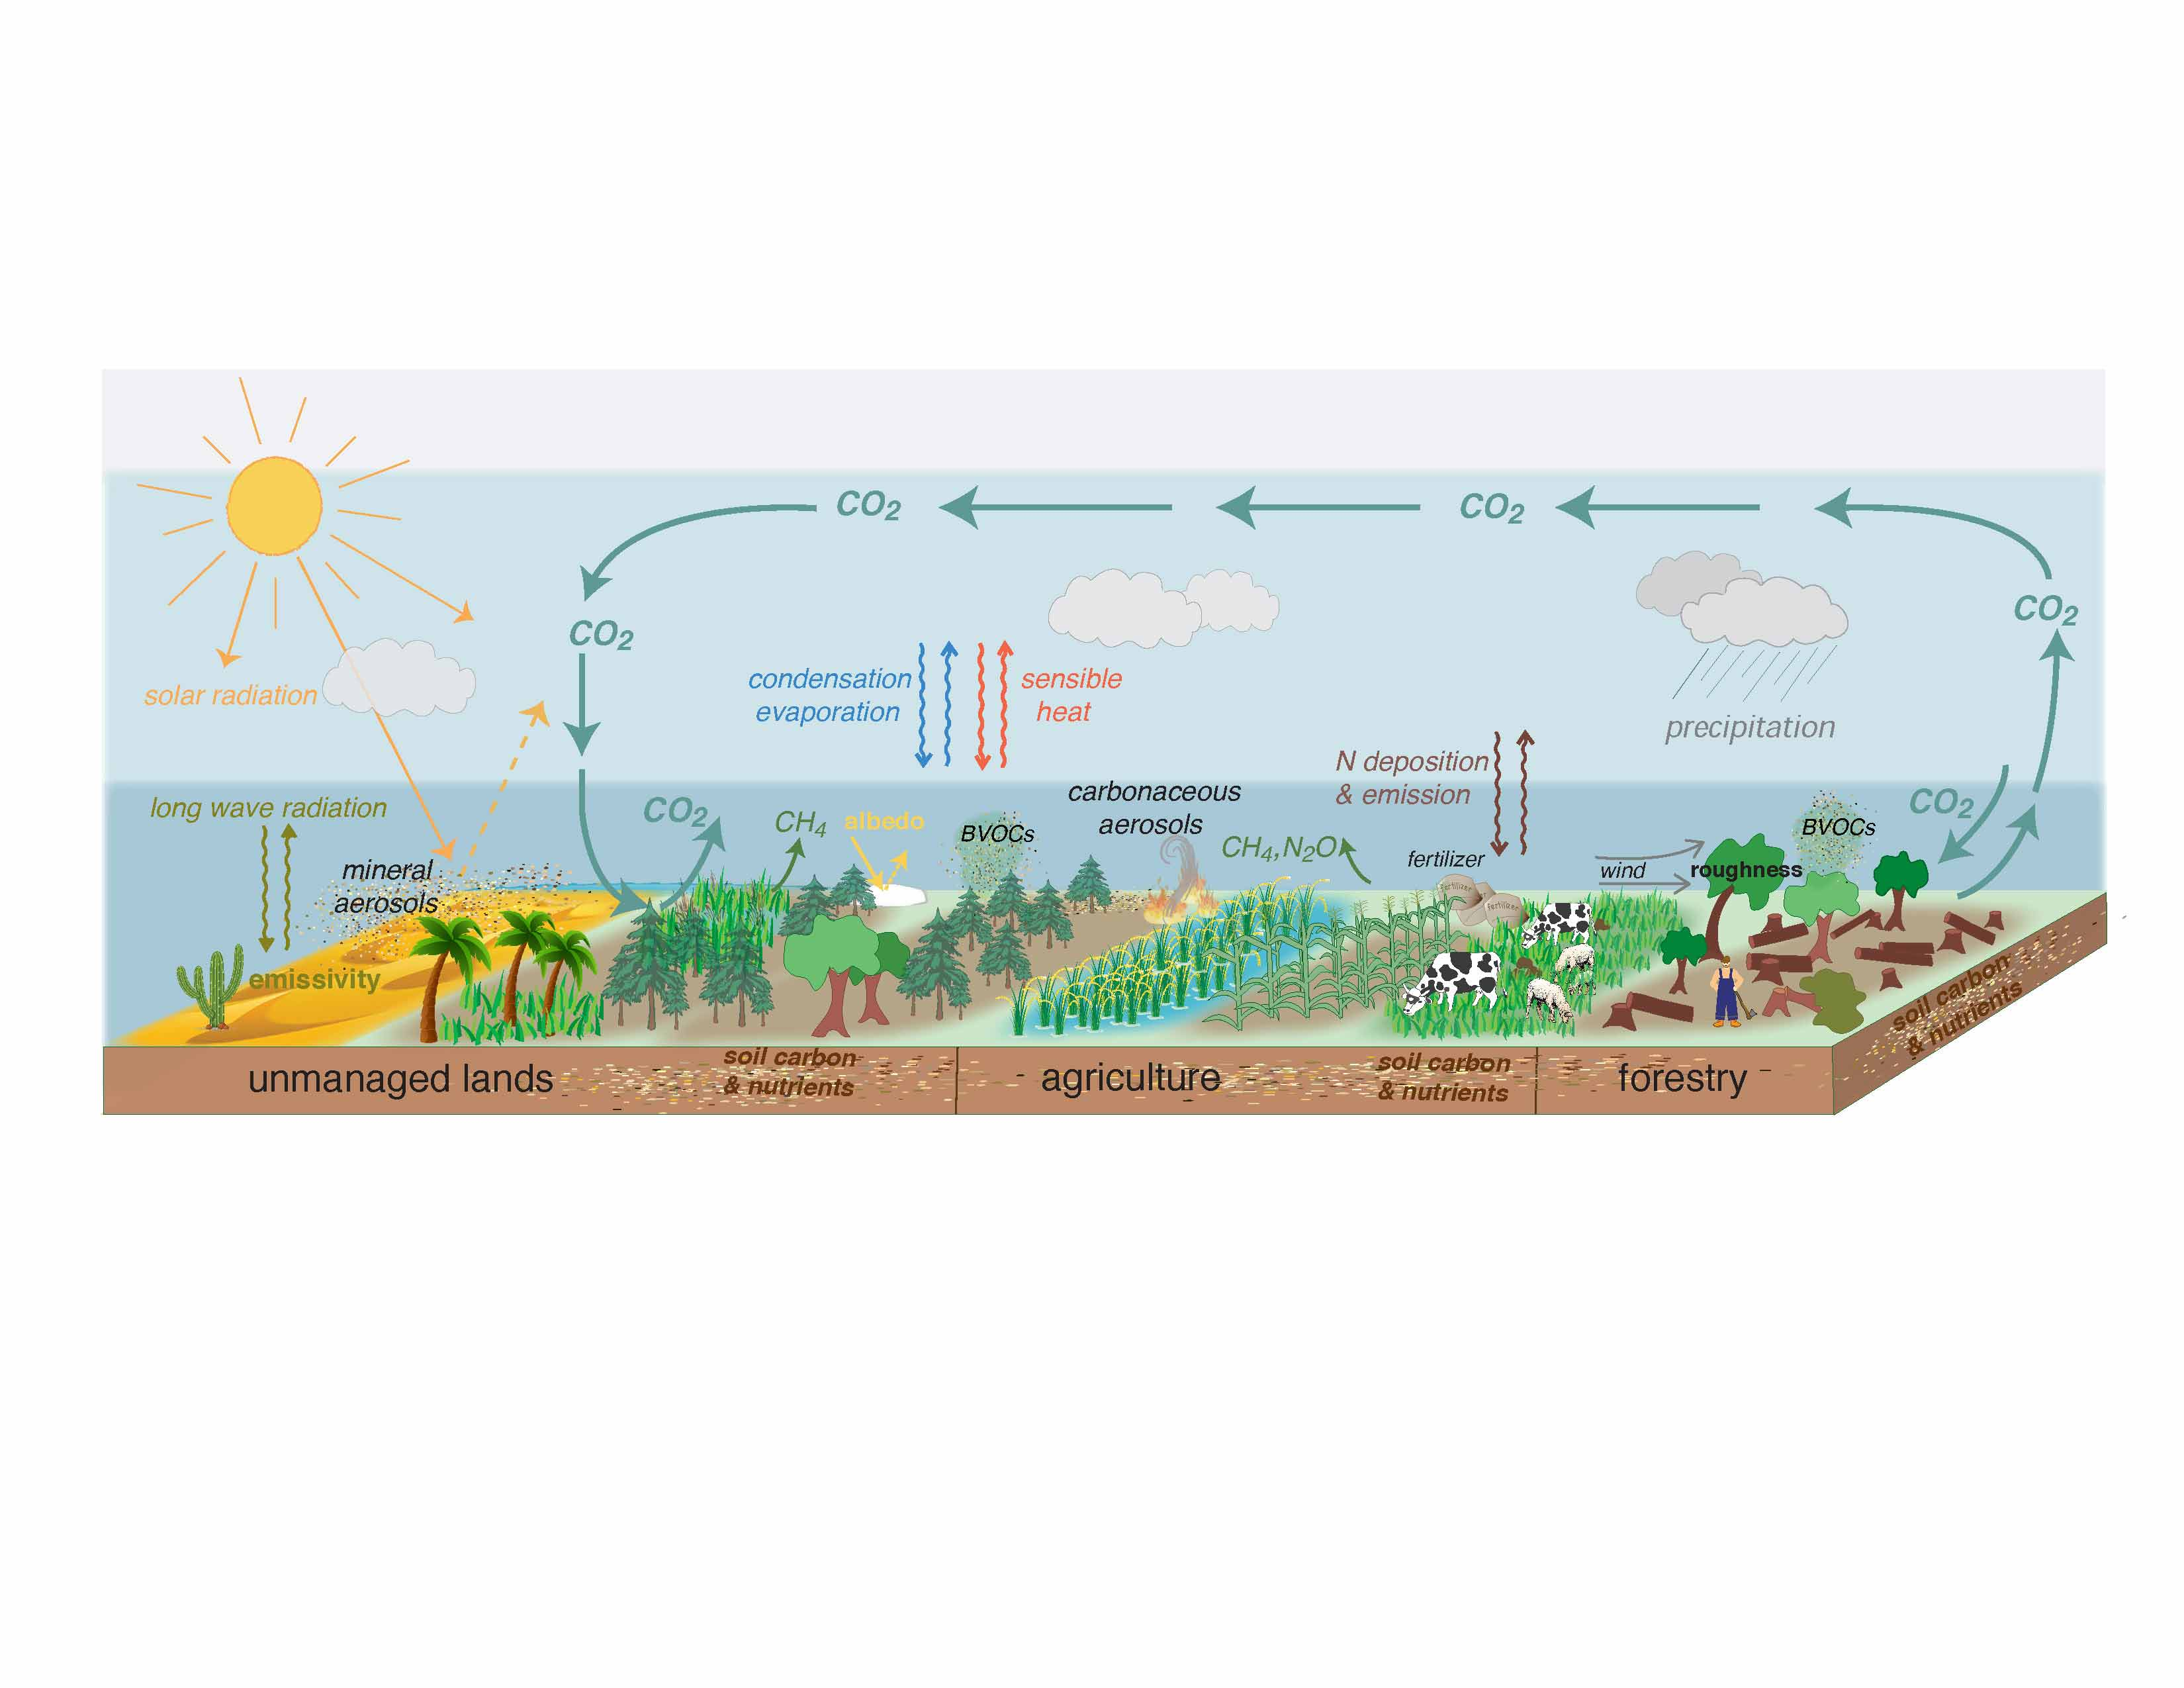
\includegraphics[keepaspectratio]{3_ecological-sustainability/images/Images_en/Fig3_11__LandClimateInteraction.png}}

}

\caption{\label{fig-land-climate-interaction}Land Climate Interaction (
05\_Chapter-2-V6.pdf (ipcc.ch))}

\end{figure}%

Beyond their impact on climate-relevant greenhouse gas flows, land use
and land use change also disrupt other \textbf{biogeochemical material
cycles}, such as nitrate, phosphorus, or sulphur cycles, linking them to
another already-exceeded planetary boundary, that of biogeochemical
flows (Richardson et al.~2023). A classic example of this is
\textbf{eutrophication}, a process that occurs when agricultural
fertilizer, such as phosphorus, enters nutrient-poor waters and leads to
excessive growth of algae, known as algal blooms. As these blooms
decompose, they deplete the oxygen level, ultimately restricting or even
preventing aquatic life (Smith et al.~2006; Galloway et al.~2008).

\begin{tcolorbox}[enhanced jigsaw, left=2mm, arc=.35mm, titlerule=0mm, opacityback=0, leftrule=.75mm, title={Tip}, breakable, bottomtitle=1mm, rightrule=.15mm, coltitle=black, toptitle=1mm, bottomrule=.15mm, colback=white, opacitybacktitle=0.6, colbacktitle=quarto-callout-tip-color!10!white, toprule=.15mm, colframe=quarto-callout-tip-color-frame]

\textbf{Land use change in the tropics: the case of Madagascar} In the
tropics, the forms of agriculture best adapted to local conditions
(i.e.~without fertilizers or other inputs) are agroforestry and
slash-and-burn agriculture. \textbf{Agroforestry} is a permanent land
use system in which annual crops are planted alongside trees, or where
perennial crops (e.g.~manioc, vanilla, bananas, and lychee) are planted
together. By contrast, \textbf{slash-and-burn agriculture}, also known
as \textbf{shifting agriculture}, refers to a land use system where a
different area is cleared each year and a crop such as maize is grown,
while the previously cultivated fields are left fallow to allow
nutrients to rebuild.

As mentioned above, slash-and-burn agriculture, such as that practiced
in Madagascar, is one of the main causes of global deforestation, which
is why governments and NGOs have been fighting slash-and-burn
agriculture since colonial times. One challenge with slash-and-burn
agriculture is that when fallow periods become too short due to a lack
of land, farmers expand into unused forest, clearing it to maintain the
cycle of slash-and-burn. This deforestation results in substantial
biomass that needs to be burnt. In Madagascar, for example, more than
6,000 burnt areas were recorded within one month from mid-September to
mid-October 2023.

This is why deforestation in Madagascar is blamed on the local
population. But slash-and-burn agriculture is a necessary survival
strategy for local inhabitants, who have few alternatives and rely on it
to secure land for future generations. This conflict of objectives is
specifically a \textbf{land use conflict}.

\end{tcolorbox}

\begin{tcolorbox}[enhanced jigsaw, left=2mm, arc=.35mm, titlerule=0mm, opacityback=0, leftrule=.75mm, title={Tip}, breakable, bottomtitle=1mm, rightrule=.15mm, coltitle=black, toptitle=1mm, bottomrule=.15mm, colback=white, opacitybacktitle=0.6, colbacktitle=quarto-callout-tip-color!10!white, toprule=.15mm, colframe=quarto-callout-tip-color-frame]

\textbf{Land use conflicts in Switzerland: the Solar Express} Another
example of a land use conflict can be observed in Switzerland, in a
conflict of interest between a decentralized renewable energy project
and landscape services (see Kienast et al.~2017). In 2022, the Swiss
government launched a ``solar offensive'' in the form of a project
called ``Solar Express''. The aim was to promote alpine photovoltaic
systems through high subsidies that would cover up to 60\% of investment
costs. In the summer of 2024, the groundbreaking ceremony for the first
large-scale plant, covering an area of 300,000 m\textsuperscript{2},
took place in Sedrun, in Switzerland's easternmost canton of Graubünden.
However, such large-scale solar plants clash with other land uses,
particularly affecting agricultural land, nature conservation areas, and
tourist regions. Solar installations alter landscapes and could affect
flora and fauna, leading to fears among farmers and nature conservation
organizations about the loss of valuable farmland and biodiversity
areas. At the same time, supporters of renewable energies are calling
for the rapid implementation of these projects, to reduce Switzerland's
dependency on fossil fuels and protect the climate. This highlights the
tension between the need for renewable energy on the one hand, and the
desire to preserve the landscape and the environment on the other.

\end{tcolorbox}

Deforestation in tropical regions is a form of land use change that is
influenced not only by local needs, but also by international decisions
and demands (Curtis et al.~2018). This suggests that preventing
deforestation must be addressed at both local and international levels
(DeFries et al.~2010). However, distant factors influence not just
deforestation, but land use change in general (Meyfroidt et al.~2013).
In science, such phenomena and processes are referred to as
\textbf{telecoupling} (Liu et al.~2013). Telecoupling describes the
socio-economic and ecological interactions between distant human and
natural systems, analysing how actions in one place (the sending system)
can affect another place (the receiving system). For example, new EU
regulations require that products entering the EU market from the end of
2024 are deforestation-free
(\href{https://environment.ec.europa.eu/topics/forests/deforestation/regulation-deforestation-free-products_en}{Regulation
on Deforestation-free products - European Commission (europa.eu)}. These
regulations are likely to have significant ecological (and social)
effects in the countries of cultivation
(https://glp.earth/news-events/blog/telecoupled-implications-new-eu-regulation-deforestation-free-products-eudr-0).

\begin{tcolorbox}[enhanced jigsaw, left=2mm, arc=.35mm, titlerule=0mm, opacityback=0, leftrule=.75mm, title={Note}, breakable, bottomtitle=1mm, rightrule=.15mm, coltitle=black, toptitle=1mm, bottomrule=.15mm, colback=white, opacitybacktitle=0.6, colbacktitle=quarto-callout-note-color!10!white, toprule=.15mm, colframe=quarto-callout-note-color-frame]

\textbf{Infobox: Land rights and land tenure}

Land use and land use change are closely linked to issues of
\textbf{land rights} and \textbf{land tenure}, as these factors largely
determine who is authorized to use land, and how it is used. Secure land
tenure and clearly defined land rights are crucial for sustainable land
use practices, as they incentivize long-term investment in land
management and promote the protection of resources. Insecure or unclear
land rights, on the other hand, can lead to land use changes that harm
the environment, such as uncontrolled deforestation. These issues become
particularly explosive in the context of \textbf{land grabbing}, in
which large areas of land are acquired by foreign (or even domestic)
investors, often without adequate consultation with or compensation for
the local population. Land grabbing can lead to conflicts that undermine
existing land rights and change land use in a way that jeopardizes
environmental and social sustainability.

\end{tcolorbox}

This chapter has shown that land, land use, and land use change are a
multifaceted topic. Underscoring the importance of this issue, Meyfroidt
et al.~(2022) summarized ten facts about land systems for sustainability
(Figure~\ref{fig-ten-facts}, left), grounded in empirical research.
These facts, in turn, lead to ten associated challenges (see Meyfroidt
et al.~2022). For example, Fact 2 (``\emph{land as complex systems}'')
leads to the challenge that the consequences of interventions in land
systems are difficult to predict and understand, which makes it
difficult to develop effective measures or policies regarding land use.
Several issues discussed in this chapter align with these facts, such as
telecoupling and Fact 5, ``\emph{Distant connections}''.

\begin{figure}[H]

\centering{

\pandocbounded{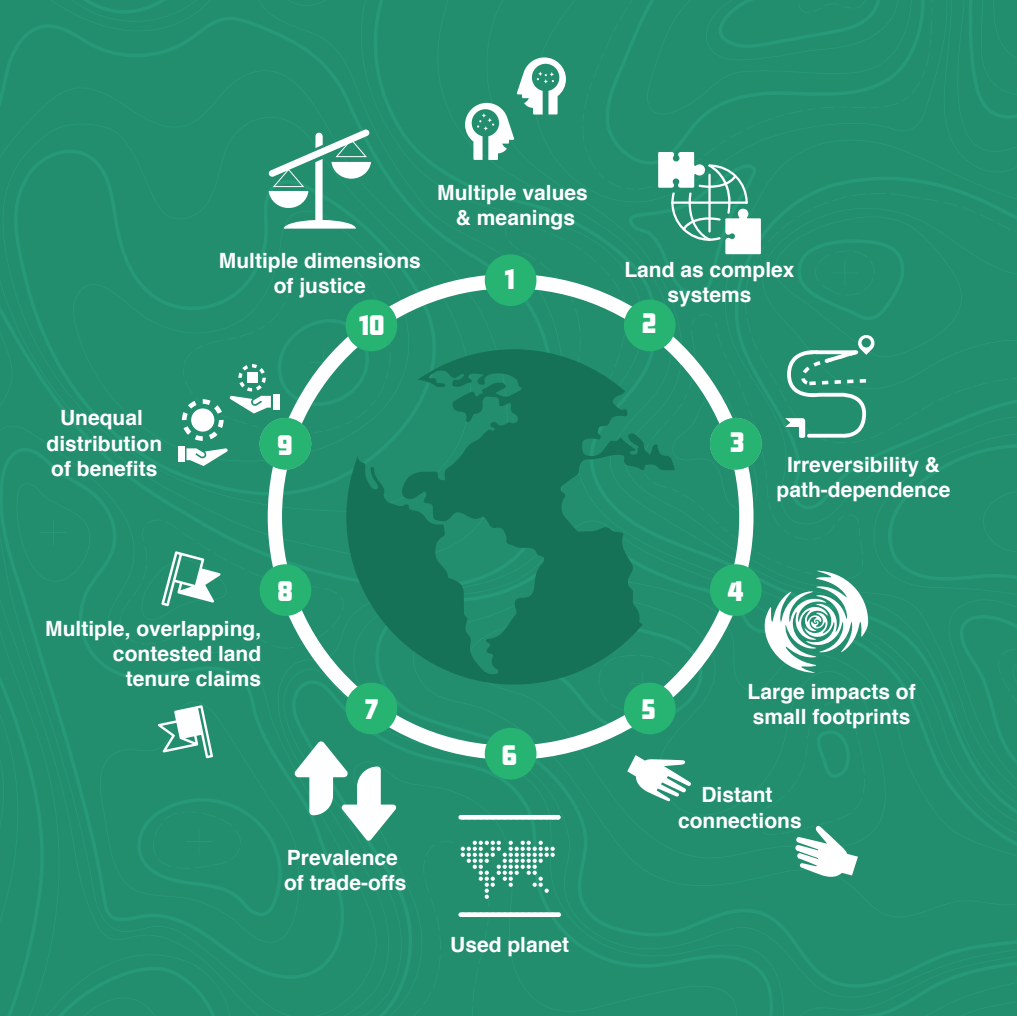
\includegraphics[keepaspectratio]{3_ecological-sustainability/images/TenFactsaboutLandSystems.png}}

}

\caption{\label{fig-ten-facts}Ten facts about land system science
(Source: Meyfroidt et al.2022)}

\end{figure}%

\begin{tcolorbox}[enhanced jigsaw, left=2mm, arc=.35mm, titlerule=0mm, opacityback=0, leftrule=.75mm, title={Tip}, breakable, bottomtitle=1mm, rightrule=.15mm, coltitle=black, toptitle=1mm, bottomrule=.15mm, colback=white, opacitybacktitle=0.6, colbacktitle=quarto-callout-tip-color!10!white, toprule=.15mm, colframe=quarto-callout-tip-color-frame]

\emph{Example: Land investments in Laos}

Another example of land use change and its far-reaching implications is
commercial land investment in Laos. The Lao People's Democratic Republic
is a mountainous, landlocked country with a high poverty rate and a few
small urban centres. Situated tween China, Vietnam, Thailand, Cambodia,
and Myanmar, Laos emerged from its communist isolation in the 1990s. The
country is rich in natural resources such as land, forests, and
minerals. To promote national economic growth, the Government of Laos is
pursuing a strategy of ``\textbf{turning land into capital}'',
i.e.~converting ``unused'' land into productive land in the hope of
achieving rural development through spillover effects. This strategy is
mainly implemented through commercial land investments, where the
government grants land concessions to domestic and foreign investors.

But to what extent does this policy actually contribute to sustainable
development? To find out, scientists from the Centre for Development and
Environment (CDE) worked with the Government of Laos to take stock of
land concessions and examine the quality of the investments. A national
digital information system was developed, enabling Laos to manage its
land concessions effectively. The system also revealed that not all
investors fulfil their promises, calling into question the
sustainability of this land use strategy.

The changes in land use towards banana plantations, other tree
plantations such as rubber plantations, mines, and hydropower projects
have led, among other things, to a loss of forest areas, with around a
third of all concessions being granted within national forest areas.
This also led to a loss of important ecosystem services and a reduction
in biodiversity. Beyond the ecological impact on the local environment,
the land investments also had socio-economic consequences. Despite
increased financial income for some, the land investments negatively
affected the well-being of the local population in many areas, reducing
food security and access to land and natural resources vital to
subsistence-oriented livelihoods.

Nanhthavong et al.~(2021), Hett et al.~(2020), CDE Policy Briefs.~

Video: \href{https://www.youtube.com/watch?v=bjogk0f99Lc}{Auf dem Weg zu
nachhaltigeren Land-Investitionen in Laos}

\end{tcolorbox}

\section{Biodiversity loss}\label{biodiversity-loss}

Biodiversity is defined as the variety of life in all its forms, ranging
from genes to species to ecosystems (CBD, 1992). It is an essential
foundation for the well-being of humankind and thus a substantial
component of \textbf{environmental sustainability}, forming the basis
for numerous ecosystem services (Haines-Young and Potschin-Young, 2010)
or Nature's Contribution to People (Antunes et al.~2024). Biodiversity
is also closely linked to several of the \textbf{planetary boundaries},
especially land-system change and biosphere integrity (Steffen et
al.~2015). It is clear that an unchecked loss of biodiversity could
trigger tipping points in ecosystems, disrupting the Earth's balance and
severely impairing the ability of our planet to support human life. The
protection and restoration of biodiversity is therefore considered key
to a sustainable future.

Yet \textbf{biodiversity} is currently in an alarming state (see infobox
below). Worldwide, species diversity has been declining for several
decades (Butchart et al.~2010; Díaz et al.~2019), a downward trend that
is predicted to continue (Díaz and Malhi, 2022). As a result, there is
already discussion of a sixth mass extinction (Ceballos et al.~2020). To
counteract this development, the \textbf{Convention on Biological
Diversity (CBD)} was ratified at the 1992 Rio Earth Summit (CBD, 1992),
with Swiss participation. This legally binding agreement means that if
Switzerland sends delegates to subsequent conferences, any new
provisions must be legally implemented.

\begin{tcolorbox}[enhanced jigsaw, left=2mm, arc=.35mm, titlerule=0mm, opacityback=0, leftrule=.75mm, title={Note}, breakable, bottomtitle=1mm, rightrule=.15mm, coltitle=black, toptitle=1mm, bottomrule=.15mm, colback=white, opacitybacktitle=0.6, colbacktitle=quarto-callout-note-color!10!white, toprule=.15mm, colframe=quarto-callout-note-color-frame]

Infobox: \textbf{Monitoring}

Biodiversity monitoring is an important tool for tracking changes in
biodiversity. The International Union for Conservation of Nature
(IUCN)'s Red List of Threatened Animal and Plant Species, maintained
since 1964, plays a particularly important role in this. It categorizes
the status of a species into one of nine categories, from ``not
endangered'' to ``extinct''. Figure \textbf{?@fig-IUCN-red-lis}, for
example, shows the percentage of species in each category at the global
level. The same categories are also used in Switzerland. Such databases,
among other benefits, help improve policymaking and nature conservation
planning, and facilitate more appropriate allocation of (financial)
resources in research and society. Despite the extensive and established
monitoring of species, cautious studies assume that only between 1.5\%
and 18\% of terrestrial vertebrate species on our planet have been
identified and described (cf.~Moura and Jetz, 2021).

\begin{figure}[H]

\centering{

\pandocbounded{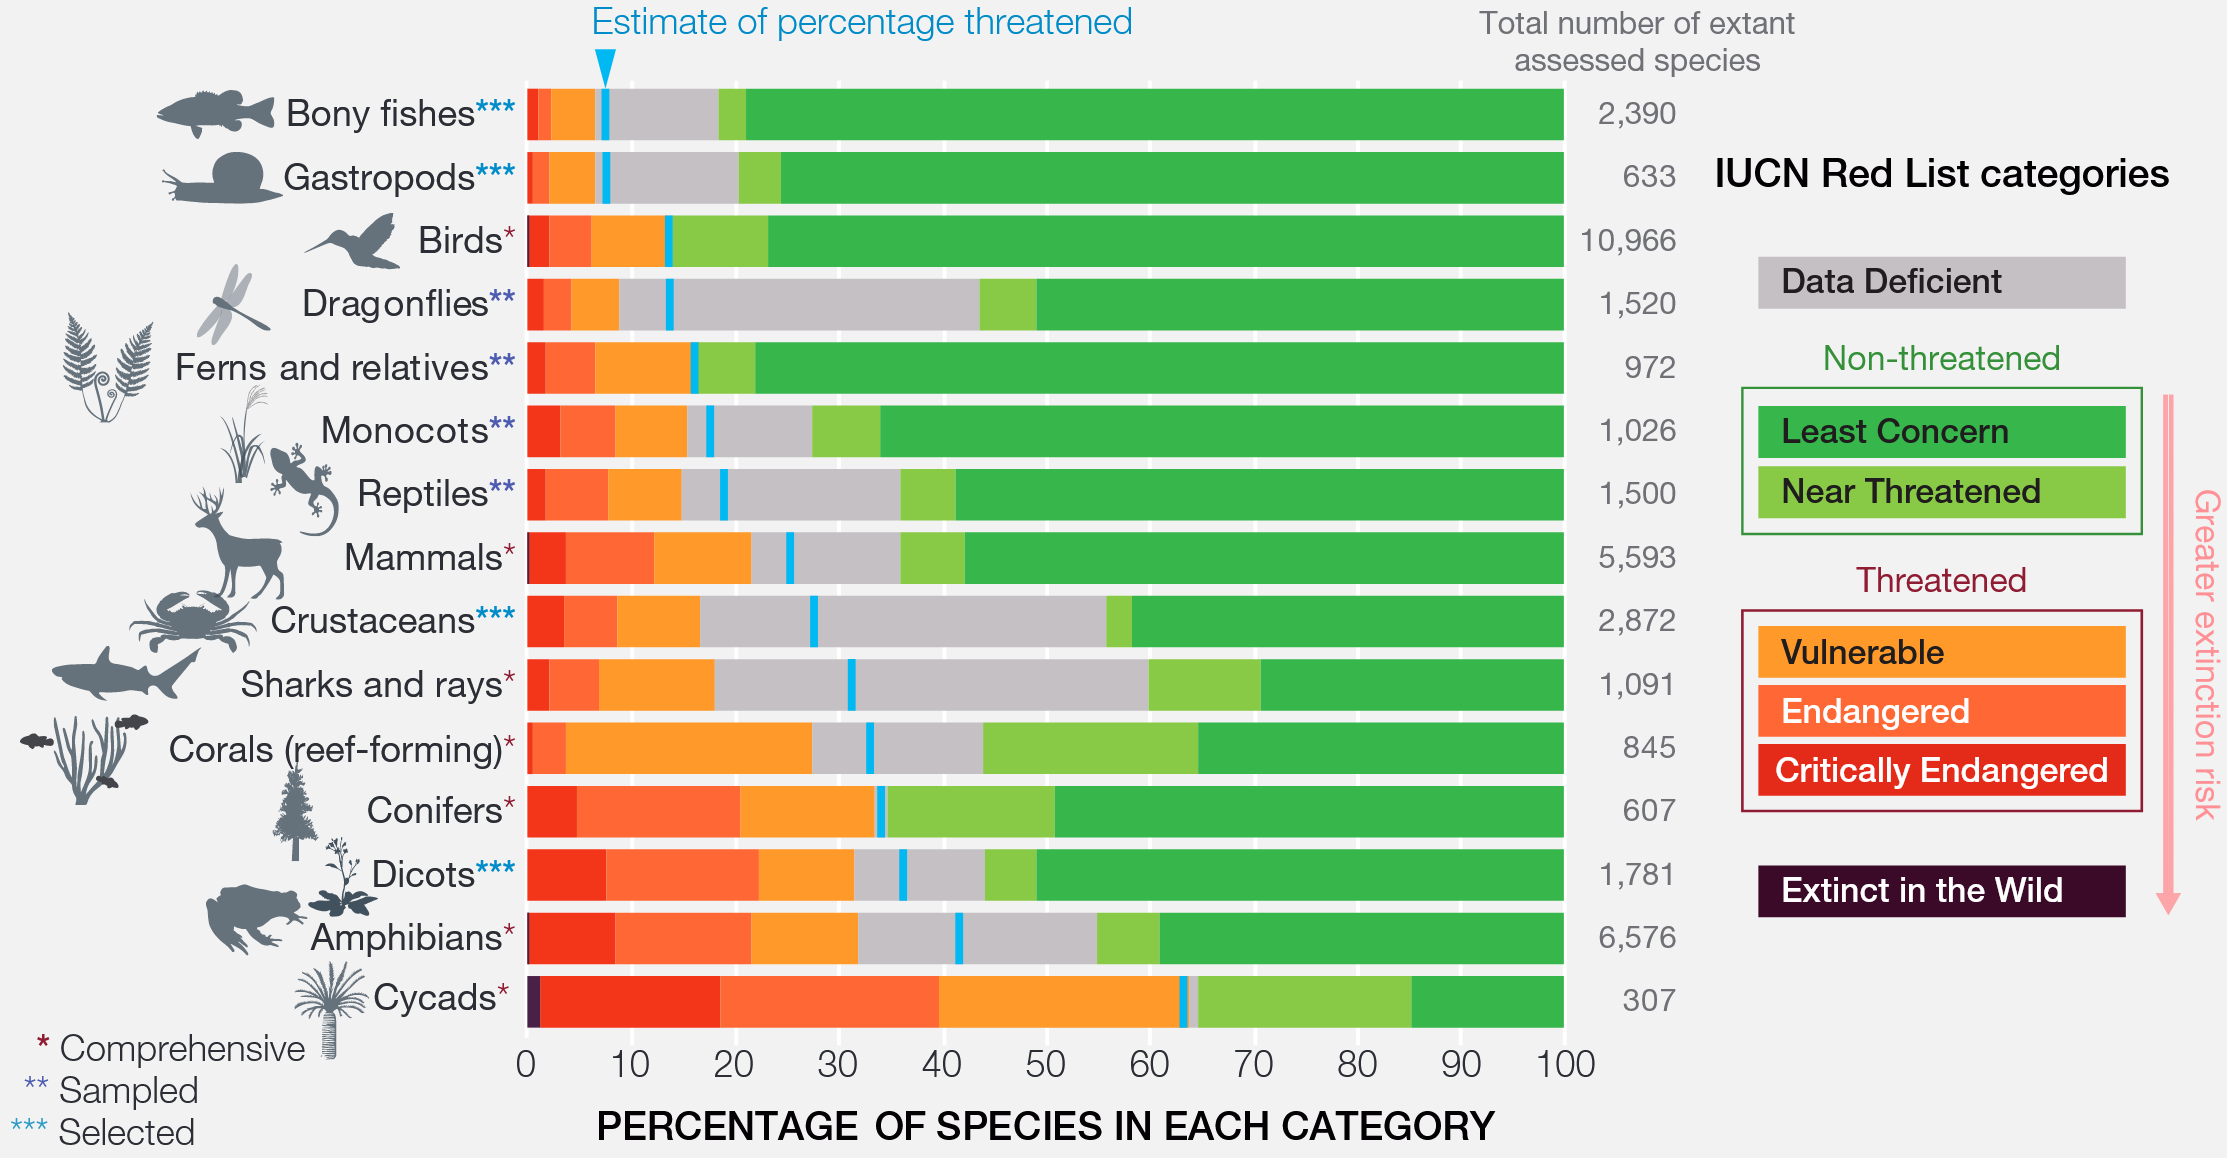
\includegraphics[keepaspectratio]{3_ecological-sustainability/images/IUCNRedList.png}}

}

\caption{\label{fig-IUCN-red-list}IUCN Red List (Source: IPBES 2019:26}

\end{figure}%

\end{tcolorbox}

Despite such international efforts, global biodiversity has been and
continues to be under unprecedented pressure. This is due to direct and
indirect \textbf{drivers} (Figure~\ref{fig-drivers-biodiversity-loss})
that have significantly accelerated over the past 50 years (IPBES, 2019:
25). For example, human activities such as \textbf{land use change} (see
Chapter XX) have drastically altered and reduced natural habitats,
leading to a significant loss of species and genetic diversity (Pereira
et al.~2010). In addition, species loss is also closely linked to
anthropogenic \textbf{climate change} (see chapter), as rising
temperatures are making or will make many areas and regions
uninhabitable for certain species (WWF, 2022: 16). This decline
jeopardizes not only the stability of ecosystems, but ultimately also
the long-term sustainability of human societies (Cardinale et al.~2012).

\begin{figure}[H]

\centering{

\pandocbounded{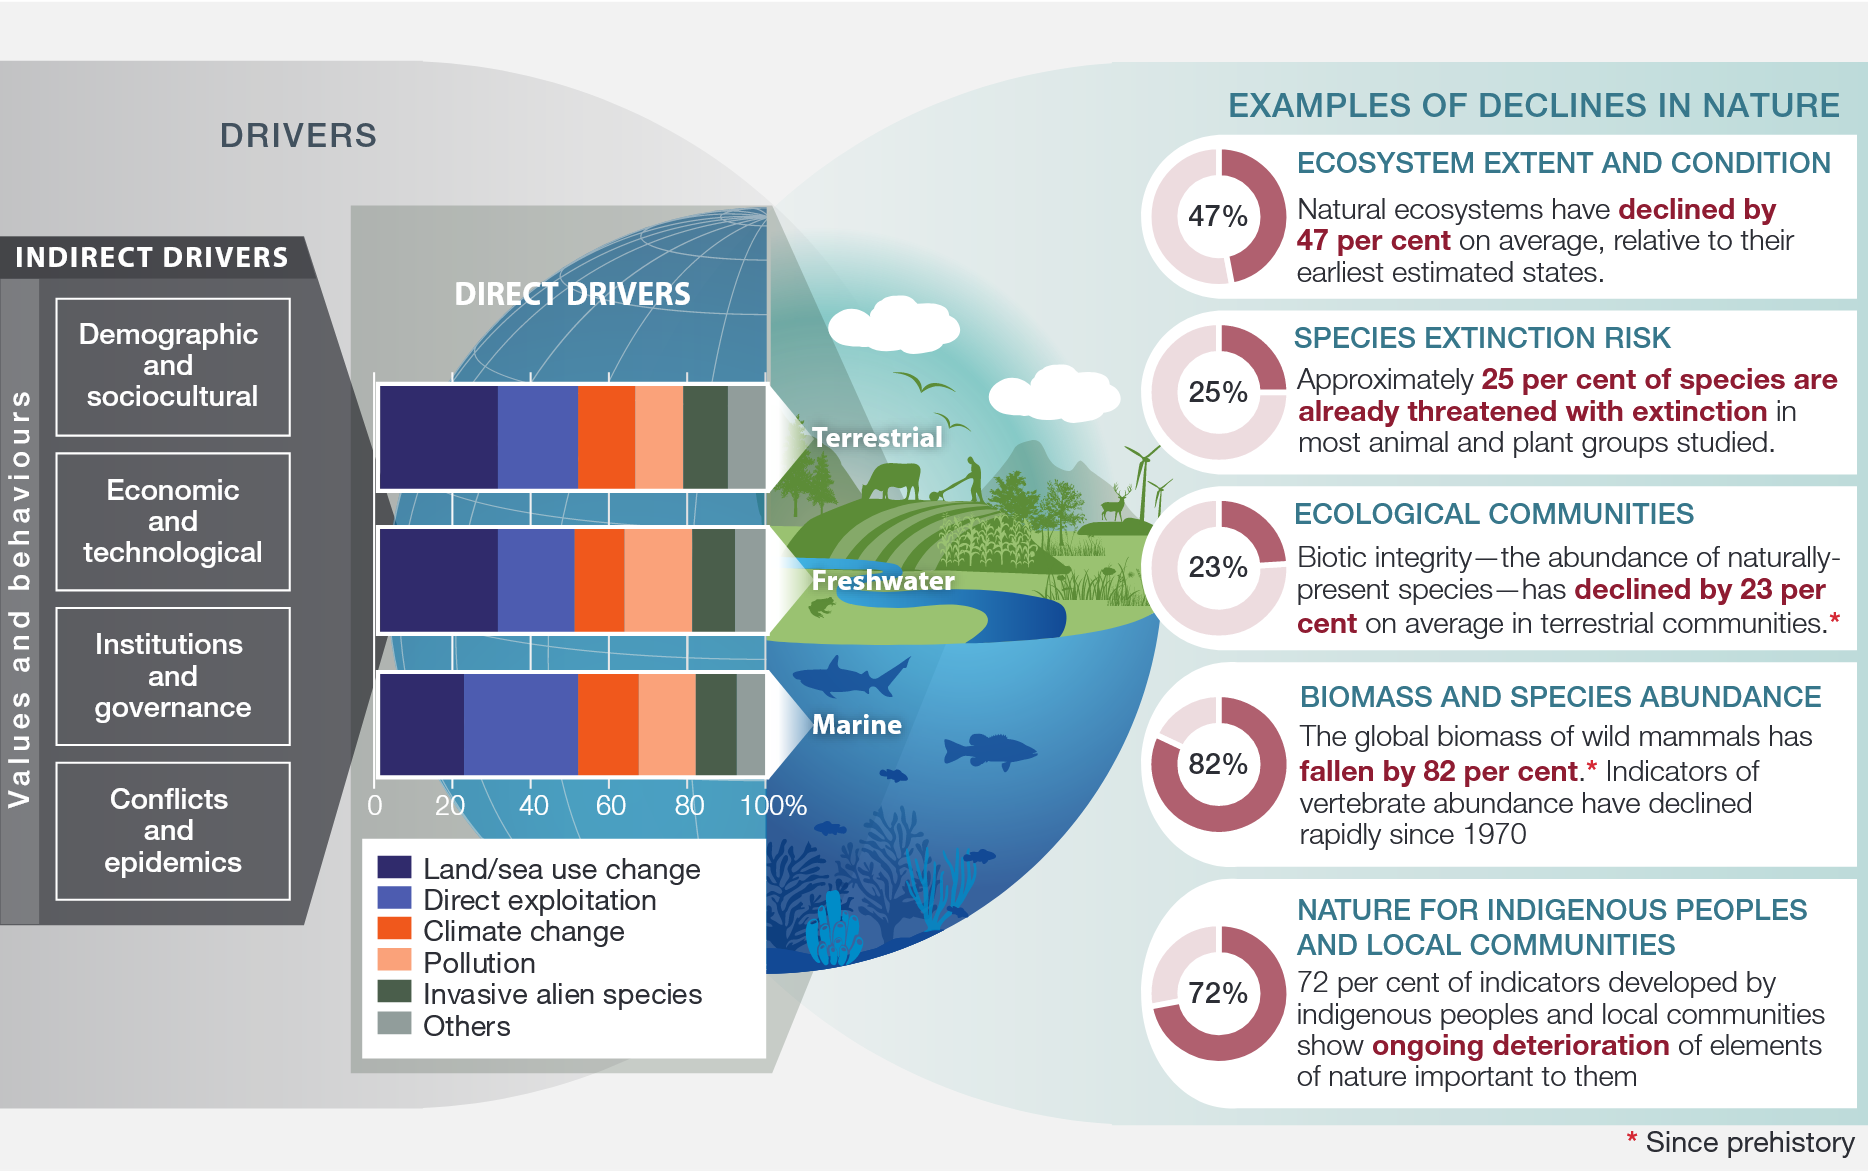
\includegraphics[keepaspectratio]{3_ecological-sustainability/images/DriversBIodLoss.png}}

}

\caption{\label{fig-drivers-biodiversity-loss}Drivers Biodiversity loss
(Source: IPBES 2019:25}

\end{figure}%

The latest major international agreement, the Kunming-Montreal Global
Biodiversity Framework (UNEP-CBD, 2022), sets new goals and targets
(Figure~\ref{fig-global-biodiversity-frame}) aimed at making global
biodiversity conservation more focused. A key target is Target 3, which
specifies that by 2030, at least 30\% of all terrestrial and marine
areas, particularly those of high ecological importance, must be
conserved through a system of \emph{protected areas}. Studies have shown
that well-managed protected areas can effectively conserve biodiversity.
However, as of 2024, only 16.32\% of terrestrial areas and 8.35\% of
marine areas were protected (\url{https://www.protectedplanet.net/en}).
More radical approaches even call for 50\% protected areas (the
\emph{Half Earth Project}).

\begin{figure}[H]

\centering{

\pandocbounded{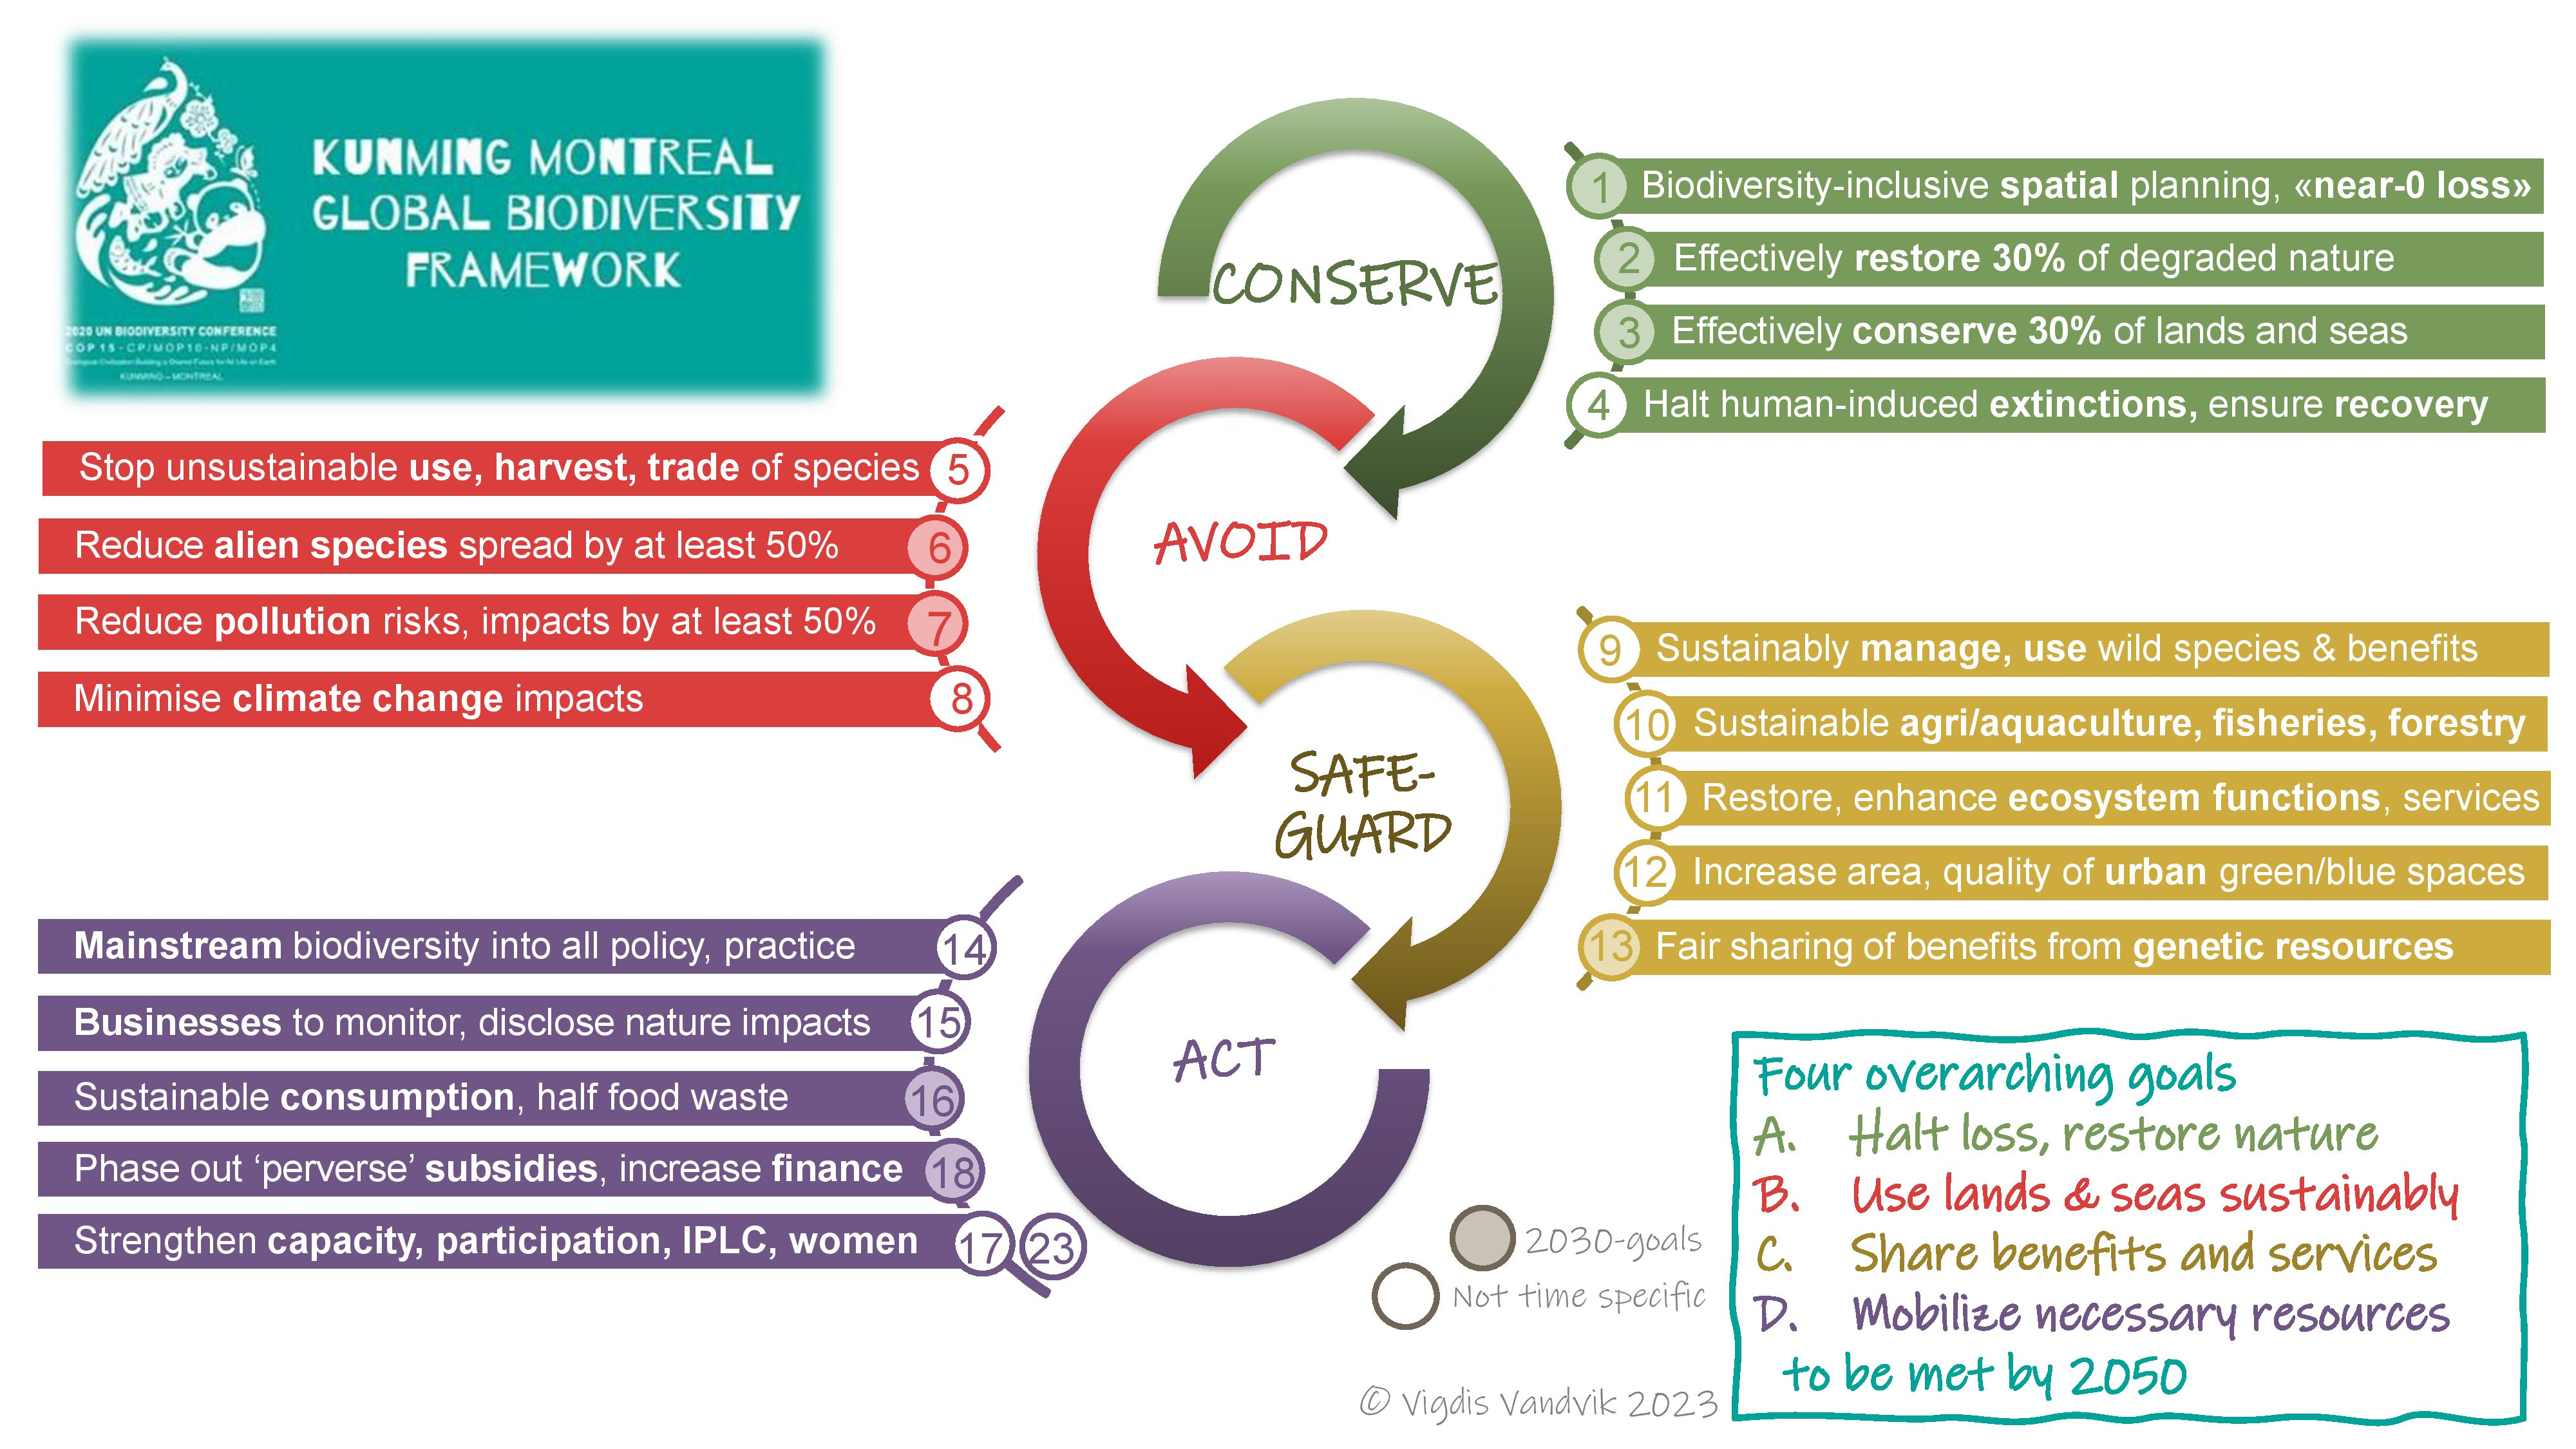
\includegraphics[keepaspectratio]{3_ecological-sustainability/images/GlobalBiodFrame.jpg}}

}

\caption{\label{fig-global-biodiversity-frame}Global Biodiversity Frane
(Source: UNEP-CBD 2022}

\end{figure}%

However, studies and scientists have voiced concern regarding the
effectiveness and (environmental) justice of \textbf{protected area and
half-earth approaches} (see Büscher et al.~2017; Schleicher et
al.~2019). Despite an increase in the surface area covered by protected
areas in recent decades, biodiversity continues to decline. On the one
hand, percentage-based targets can create false incentives, leading
governments to designate nature reserves in areas where they provide
little benefit or serve only as paper tigers (Visconti et al.~2019). On
the other hand, designation of strict protected areas often deprives
local population groups, especially Indigenous groups, of access to the
areas on which they depend for their livelihoods -- or it forces them to
resettle. Studies have shown that the participation of local population
groups is a decisive factor for the long-term conservation and integrity
of protected areas and thus of biodiversity (Andrade \& Rhodes, 2012).
IPBES (2019: 32) also recognizes the importance of Indigenous and local
communities in the conservation of biodiversity and ecosystem services.
A study by Fa et al.~(2020), for example, shows how involving Indigenous
communities can benefit nature conservation. The study illustrates that
Indigenous territories worldwide -- and especially in the tropics --
play a crucial role in protecting biodiversity and curbing
deforestation. The study compares deforestation rates in different
protected areas and shows that deforestation is significantly lower in
areas under Indigenous administration than in state-protected regions.

\begin{tcolorbox}[enhanced jigsaw, left=2mm, arc=.35mm, titlerule=0mm, opacityback=0, leftrule=.75mm, title={Note}, breakable, bottomtitle=1mm, rightrule=.15mm, coltitle=black, toptitle=1mm, bottomrule=.15mm, colback=white, opacitybacktitle=0.6, colbacktitle=quarto-callout-note-color!10!white, toprule=.15mm, colframe=quarto-callout-note-color-frame]

\textbf{What is IPBES:} The Intergovernmental Science--Policy Platform
on Biodiversity and Ecosystem Services (IPBES) is an independent
intergovernmental body established by various countries to strengthen
the science--policy interface on biodiversity and ecosystem services for
the conservation and sustainable use of biodiversity, long-term human
well-being, and sustainable development. It was founded on 21 April 2012
in Panama City by 94 governments. Secretariat services to the IPBES are
provided by the United Nations Environment Programme (UNEP), although
IPBES is not a UN body. Today, IPBES, which developed the NCP concept,
is considered a counterpart to the IPCC.
\url{https://www.ipbes.net/about}

\end{tcolorbox}

Like land use change (reference) and ecosystem services (reference),
biodiversity protection and nature conservation are caught between
various \textbf{values and visions}, which can lead to conflicts of
interest among various stakeholders. These values and the resulting
approaches are generally categorized into three types: intrinsic,
instrumental, and relational values (Durán et al.~2023): in other words,
``nature for nature'', ``nature as culture'', ``nature for society''
(Figure~\ref{fig-NFF}). The concept of ecosystem services, for example,
falls under ``\textbf{nature for society}'', as it corresponds to a
utilitarian view of nature in which society derives the greatest
possible benefit from nature (without harming it). By contrast, a nature
park that prioritizes strict nature protection or the rewilding of
areas, for example, can be classified as embodying intrinsic values,
because human intervention and thus its impact on nature is minimized.
This ``\textbf{nature for nature}'' narrative also extends to concepts
like smart cities, for example, as these seek to limit human activity to
urban areas as efficiently as possible. The ``\textbf{nature as
culture}'' vision, for its part, portrays a world where values such as
reciprocity and harmony define human relationships with nature at every
level. Here, biological diversity and cultural diversity are jointly
preserved and managed within closely linked biocultural systems. These
systems are supported by local, self-determined governance structures
that respect Indigenous sovereignty and local identities. Economic
exchange prioritizes the social value of goods over their monetary
value. This vision includes, for example, local and decentralized food
production as well as communities that operate in a resilient,
biocultural network with deep spiritual connections to nature.

\begin{figure}[H]

\centering{

\pandocbounded{\includegraphics[keepaspectratio]{3_ecological-sustainability/images/NFF (Duran et al. 2023).webp}}

}

\caption{\label{fig-NFF}The Nature Futures Framework (Source: Pereira et
al.~2020)}

\end{figure}%

The diverse values associated with biodiversity and nature -- and to
what extent they should be protected -- therefore require a normative
assessment. They are based not only on empirical systems knowledge but
also on ethical principles, as explained at the start of Chapter 3 (See
Chapter 3.1 Normative Dimension of Sustainability).

As we have seen, and as with other sustainability challenges and
dimensions, there is no established consensus on how to best implement
and achieve sustainability in the environmental dimension. In this
dimension, too, sustainable development remains a social negotiation and
decision-making process. Given the diversity of different perspectives
and interests of various stakeholders, preferences regarding approaches
and measures also vary. To select suitable measures and harmonize the
various levels of responsibility (Figure~\ref{fig-SD-ethics}), we can,
for example, refer back to Hans Jonas's (1979) ethics of responsibility,
which we learned about at the start of the book (see chapter X).
Integrating these various areas of responsibility can foster a holistic
and sustainable ethic that appropriately considers the needs and
interests of all aspects of life and nature.

\begin{figure}[H]

\centering{

\pandocbounded{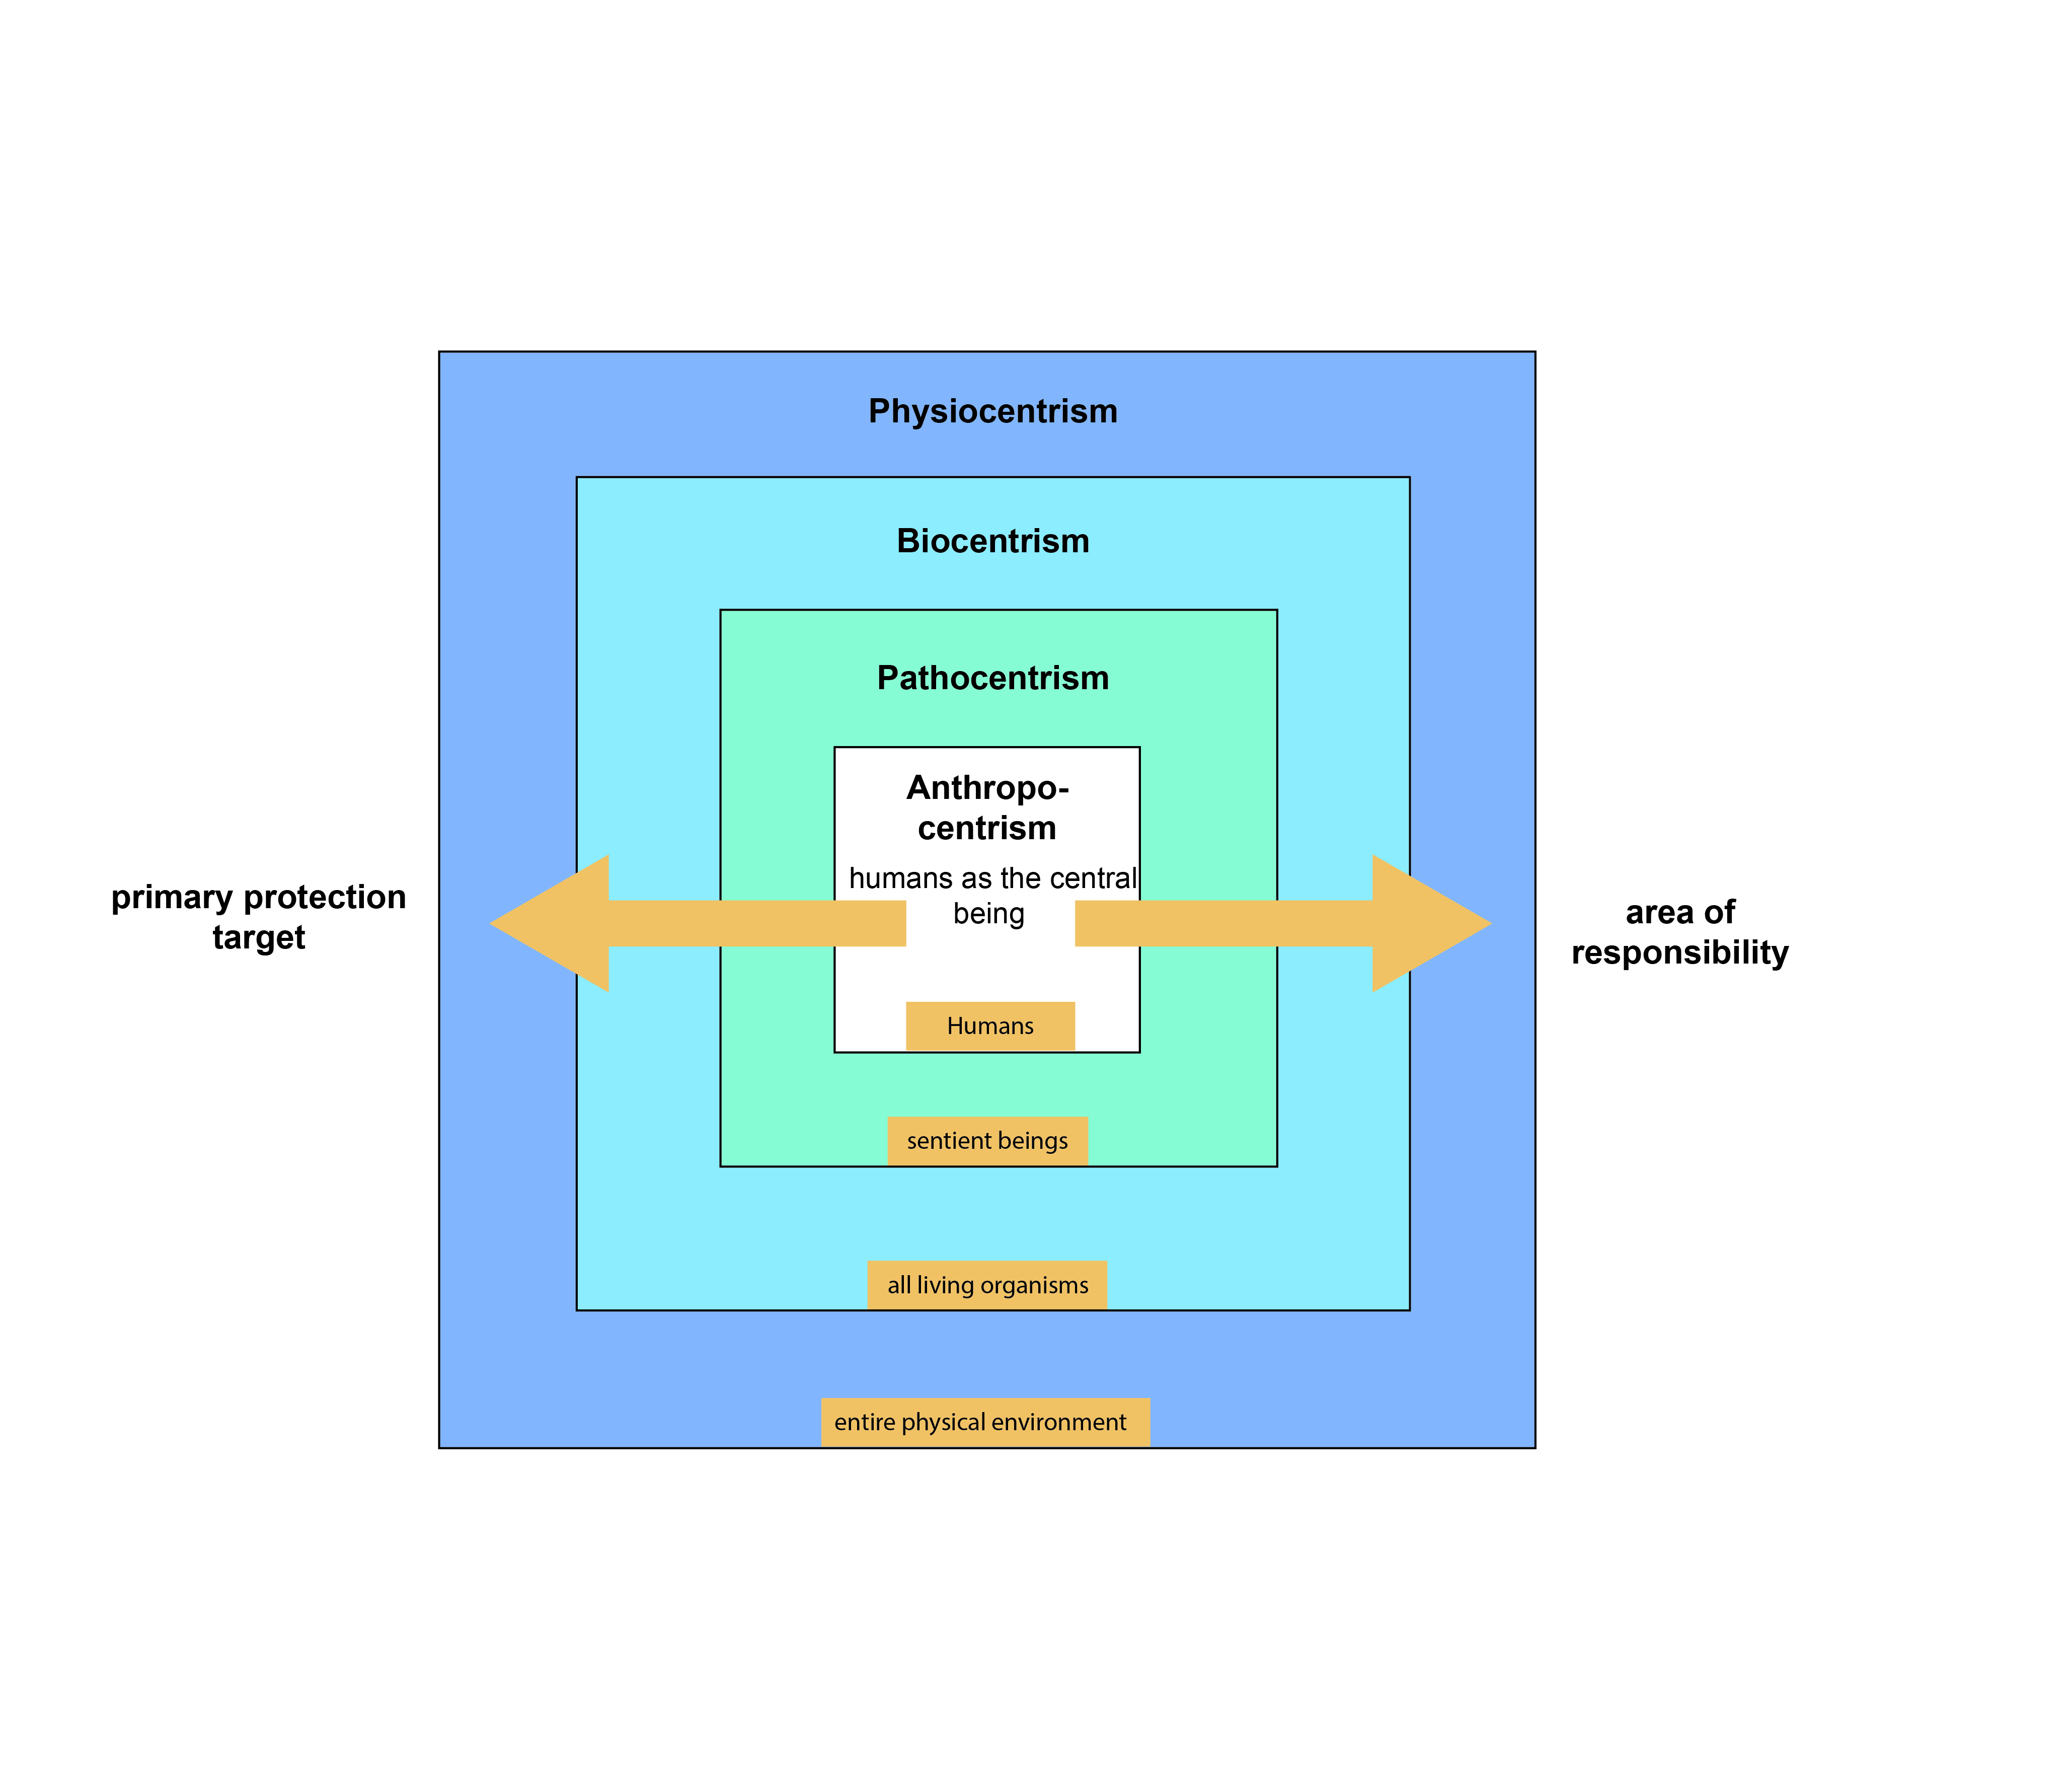
\includegraphics[keepaspectratio]{3_ecological-sustainability/images/Images_en/Fig1_8__ethics.jpg}}

}

\caption{\label{fig-SD-ethics}Sustainable Development Ethics (Quelle?)}

\end{figure}%

\section{Strategic approaches}\label{strategic-approaches}

These days, various strategies are being pursued or at least considered
to achieve a transformation in the environmental dimension of
sustainable development (see Figure~\ref{fig-GDSR} for a non-exhaustive
list). Some of these strategies were previously discussed in this
textbook. While the approaches mentioned do not necessarily have to be
transformative per se, they can certainly have an impact on the
environmental dimension of sustainability if applied appropriately. The
approaches presented in this section are categorized according to the
``Levers for Transformation'' of the Global Sustainable Development
Report (GSDR) (see chapter x). The 2019 GSDR defines four levers:
governance, economy and finance, individual and collective action, and
science and technology. The 2023 GSDR added a fifth lever, capacity
building, as this is essential for a transformative process both as a
lever itself and as a supporting factor for the other levers
(Independent Group of Scientists appointed by the Secretary-General,
2023).

For each lever, we present selected strategies related to our three
topics of focus in this Chapter, climate, land use, or biodiversity:

The \textbf{governance} lever involves institutions and spaces that
determine the direction of development by setting goals, coordinating
measures, creating regulations, and facilitating funding at national and
regional level. Good governance should also promote synergies, take into
account conflicts of interest, and strengthen cooperation between a wide
range of stakeholders. Governance thus plays a key role in the
development and implementation of environmental sustainability
strategies, as it can establish the policy framework for sustainable
practices through regulatory mechanisms, incentive structures, and laws.
Governance levers include:

\begin{itemize}
\item
  Creation of protected areas to preserve biodiversity
\item
  Subsidies for sustainable practices, such as direct payments for
  biodiversity-friendly farming methods
\end{itemize}

The \textbf{economy and finance} lever primarily refers to the
significant public and private investments required to achieve the SDGs
and transformation (globally, between USD 1.4 and 2.5 trillion per
year). This lever is thus a key enabler of environmental sustainability
strategies and policies, for example through the funding of sustainable
technologies. Examples include:

\begin{itemize}
\item
  Payments for Ecosystem Services (PES)
\item
  REDD+ programmes to reduce deforestation and promote sustainable land
  use
\end{itemize}

The \textbf{science and technology} lever refers to social and
technological innovation as well as cost-effective and scalable
technologies. This includes investing in research and development,
fostering greater international cooperation, and enabling access to
proven technologies (especially for low-income countries), where science
can help explain complex interrelationships and develop evidence-based
solutions. Essential levers for sustainability transformations include:

\begin{itemize}
\item
  Carbon sequencing technologies
\item
  Nature-based solutions that use natural processes to address climate
  change and environmental problems
\item
  Innovative land use systems, such as agroforestry\\
\end{itemize}

\textbf{Individual and collective action}\\
Social change often begins in people's hearts and minds through local
organization and mobilization before translating into laws and economic
policy. When a critical mass adopts new practices or norms, this can be
supported by education, information campaigns, financial incentives, and
legislation, and extended to the whole of society. Examples of
sustainability strategies and policies in the field of individual and
collective action include:

\begin{itemize}
\item
  Sustainable consumption campaigns that motivate consumers to choose
  environmentally friendly products
\item
  Promotion of solidarity-based farming models (SoLaWi) that strengthen
  regional and organic food production
\end{itemize}

\textbf{Capacity building\\
}Capacity building to support the transformation to achieve the SDGs is
multifaceted and depends on the goal, the required transformations, and
the specific country or regional context. Among other things,
competences are required in the areas of strategic orientation,
innovation, coordination, learning, and resilience. Environmental
sustainability strategies and policies related to the capacity building
lever include:

\begin{itemize}
\item
  Establishment of advice centres or digital platforms to enable
  continuous learning and the exchange of best practices, e.g.~in the
  field of agroforestry
\item
  Supporting local initiatives to improve knowledge transfer\\
\end{itemize}

Note: It is important to be aware that approaches aren't always
synergistic; often, an approach addressing an environmental dimension of
sustainability involves trade-offs with other approaches or with the
social or economic dimensions of sustainability.

\begin{figure}[H]

\centering{

\pandocbounded{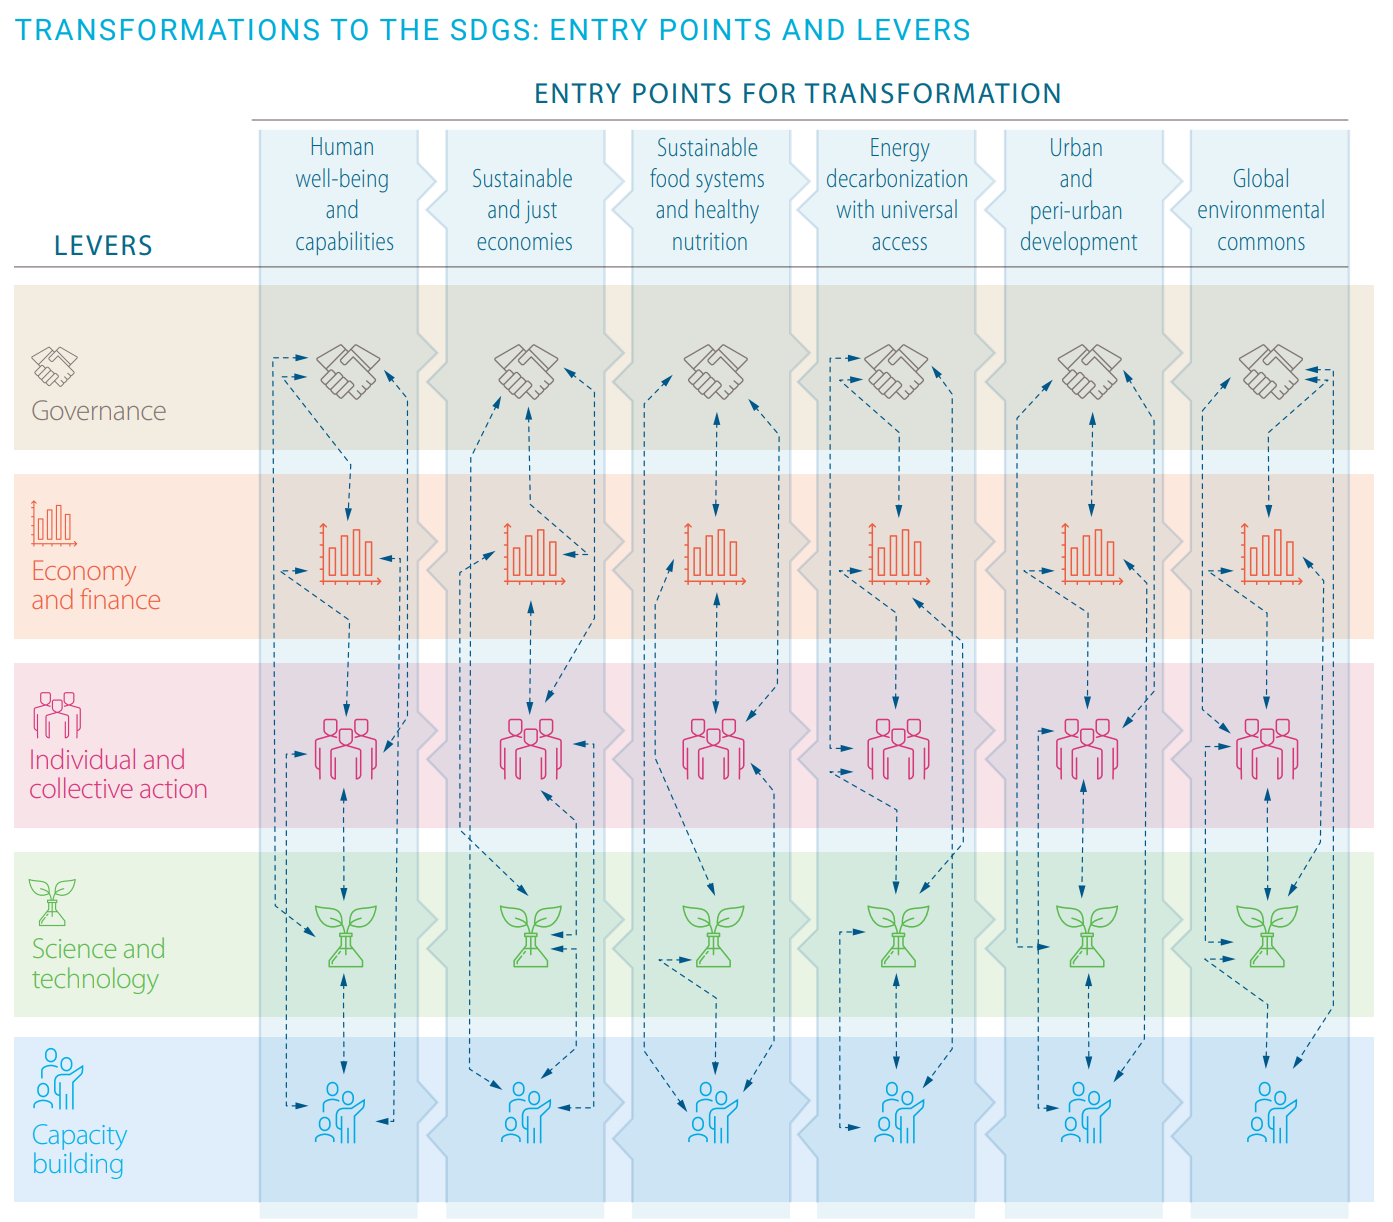
\includegraphics[keepaspectratio]{3_ecological-sustainability/images/Images_en/Fig3_17__GSDR.png}}

}

\caption{\label{fig-GDSR}GSDR (Quelle?)}

\end{figure}%

\begin{tcolorbox}[enhanced jigsaw, left=2mm, arc=.35mm, titlerule=0mm, opacityback=0, leftrule=.75mm, title={Note}, breakable, bottomtitle=1mm, rightrule=.15mm, coltitle=black, toptitle=1mm, bottomrule=.15mm, colback=white, opacitybacktitle=0.6, colbacktitle=quarto-callout-note-color!10!white, toprule=.15mm, colframe=quarto-callout-note-color-frame]

Further reading:

Guyer M., Steinemann M., and Saalismaa N. (2022), \emph{Biodiversity and
Sustainable Development}. Climate Change \& Environment Nexus Brief.
Swiss Agency for Development and Cooperation: Bern, Switzerland.

\end{tcolorbox}

\chapter{Social Sustainability}\label{social-sustainability}

\textbf{Social sustainability} is about a community's well-being,
encompassing elements like inclusion, equity, and social cohesion. It's
often argued that this dimension of sustainable development is harder to
grasp than environmental or economic sustainability (Foladori, 2005).
That's because social issues may not be as immediately visible as, say,
rainforest destruction or hyperinflation. What does sustainability mean
when communities are unequally affected through events such as flooding,
or when Indigenous peoples are displaced by infrastructure projects?
These impacts reveal deep-rooted inequalities that are largely based on
societies' social structures.

This is why the social dimension is so important. A society that is
socially sustainable is better prepared to tackle challenges fairly and
equitably (Ballet et al.~2020). Furthermore, having social acceptance is
crucial for successfully implementing sustainability measures and
initiatives (Assefa \& Frostell, 2007; Wüstenhagen et al.~2007).

In short, social sustainability addresses the following challenge: How
can we create a resource-conserving society without increasing poverty
and inequality? Achieving this requires balancing fundamental questions
of distributive justice with the tension between human needs and wants.

This chapter begins by introducing social sustainability as a normative
dimension of sustainable development. We define the concept by focusing
on the following key elements: inclusion, social cohesion, resilience,
and justice. Finally, we address the cultural aspect. While some
scholars see culture as a component of social sustainability, others
argue that it should be considered a fourth dimension in its own right
-- alongside the environmental, social, and economic dimensions
(Sabatini, 2019).

\section{Social sustainability, a normative
concept}\label{social-sustainability-a-normative-concept}

Interpretations of social sustainability are based, on the one hand, on
empirical knowledge about how societies function and, on the other, on
ethical judgements about what is valuable and should be pursued. In
order to define appropriate sustainability goals, we need to know what
ethical principles and values a particular social system is based on. In
other words, what does a society or community perceive as ``good'',
desirable, and just?

As a normative concept, social sustainability aims for a fair
distribution of benefits and costs within society. It encompasses
various dimensions of equality (see Section X) and justice (see Section
X), and it examines how the decisions made within a particular society
influence the distribution of resources.

\begin{figure}[H]

\centering{

\pandocbounded{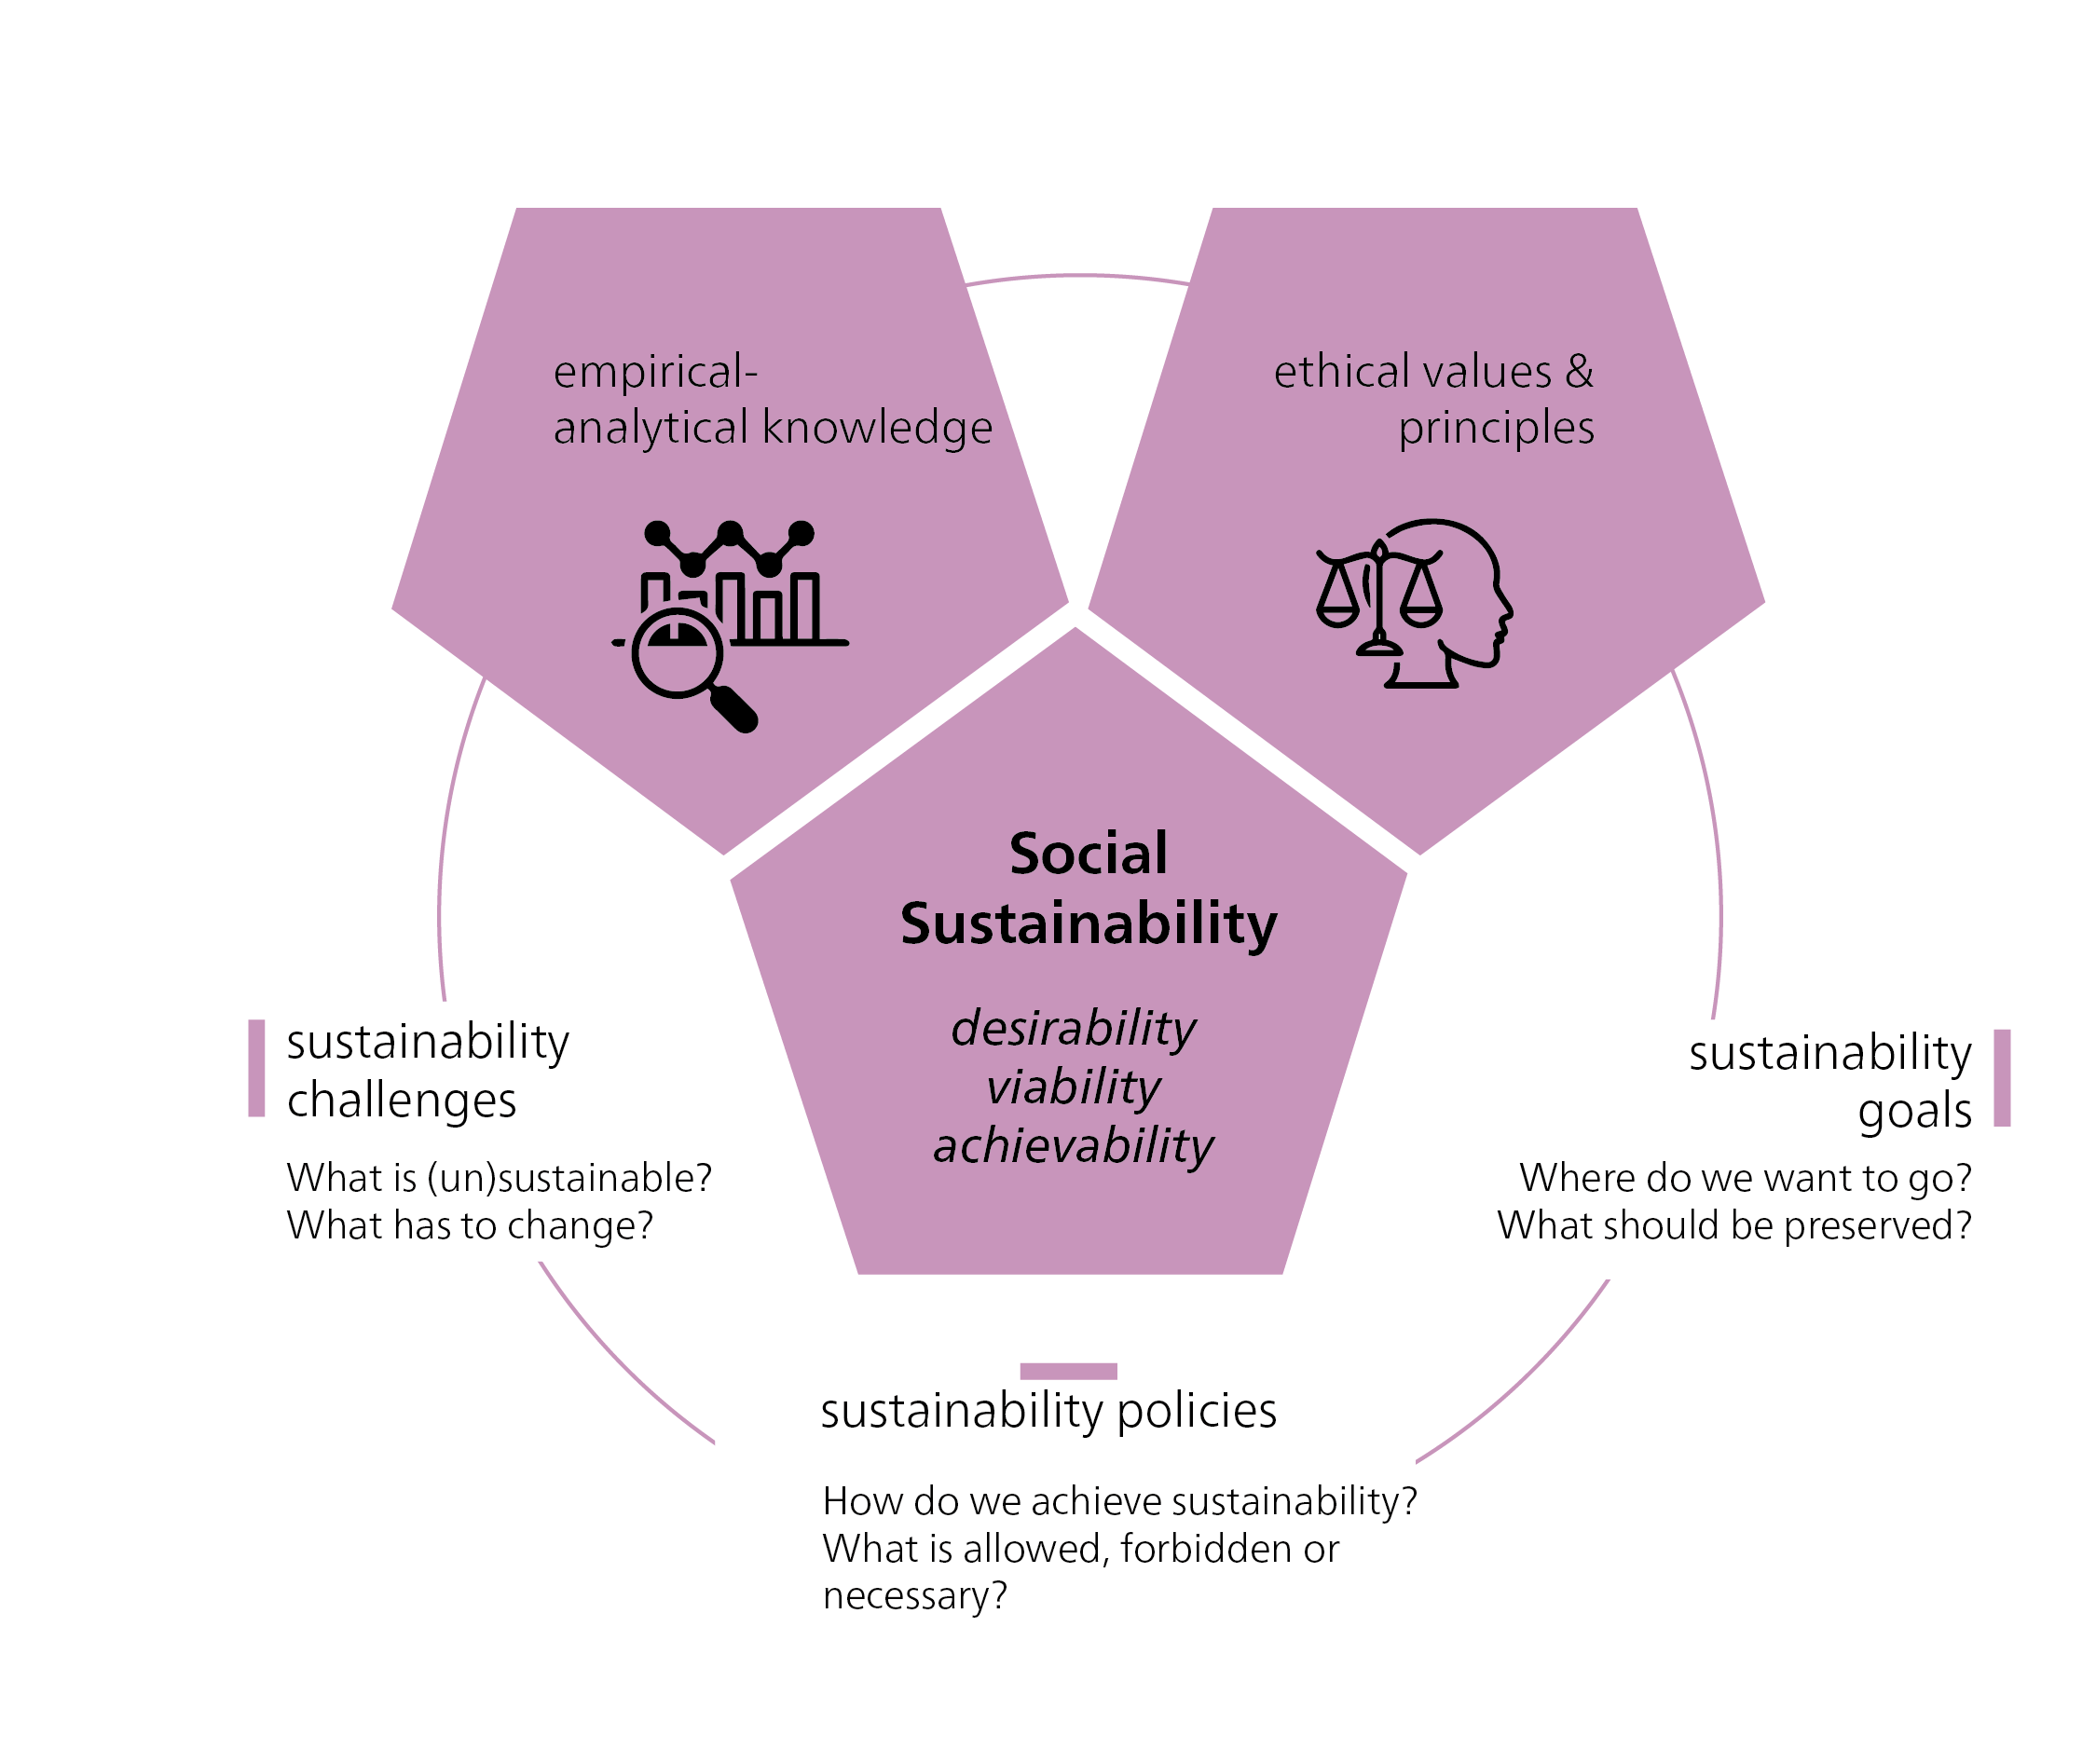
\includegraphics[keepaspectratio]{4_social-sustainability/images/Fig4_1_NESocial.png}}

}

\caption{\label{fig-NESocial}Social Sustainability. Source: Own
illustration}

\end{figure}%

These are aspects exemplified by Kate Raworth's doughnut economics
(2017; see Section 3.2), a framework which views the SDGs and human
rights as the basis for socially sustainable and equitable human
activities. In doughnut economics, meeting the basic needs of all people
is key. These basic needs, which form the framework's social foundation,
include access to clean water, sanitation, healthcare, education, food,
clean cooking facilities, electricity, housing, and information and
support networks, as well as the opportunity to work and earn an income.
Additional factors which form the social foundation are gender equality,
social equality, peace, and justice, as well as political participation
-- i.e.~the ability to exert social influence.

In doughnut economics, economic policies could contribute to achieving
social justice by distributing benefits and costs without exceeding
planetary boundaries. And therein lies the challenge: Countries that
perform well in terms of social sustainability indicators -- e.g.~access
to food, education, or housing -- often exceed ecological boundaries.
Conversely, countries that stay within these ecological limits often
score poorly in social areas (see Figure X; O'Neill et al.~2018).
Striking a balance between social and environmental requirements is
therefore key.

\begin{figure}[H]

\centering{

\pandocbounded{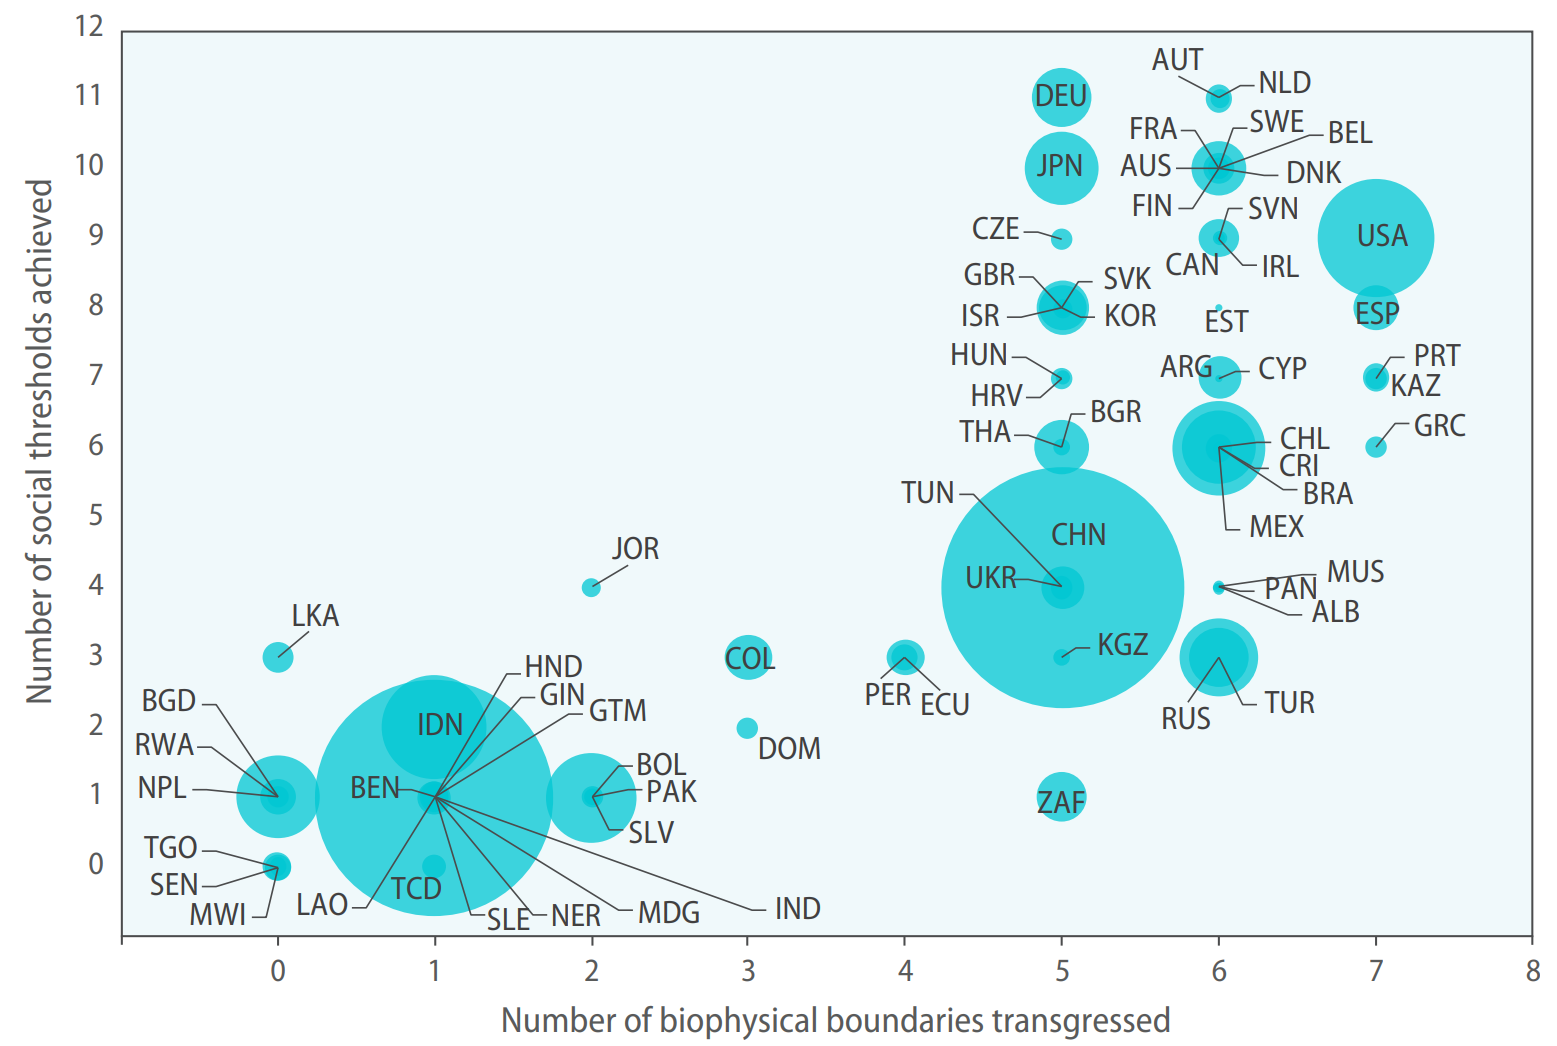
\includegraphics[keepaspectratio]{4_social-sustainability/images/Fig4_2_SocialEcologicalBoundaries.png}}

}

\caption{\label{fig-SocEcoBoundaries}Social thresholds achieved versus
biophysical boundaries transgressed for different countries, results
weighted by each country's population. Source: UN/DESA, based on O'Neill
and others (2018), figure 2.}

\end{figure}%

To achieve a sustainable future, Raworth (2017) argues that we must
distribute the Earth's resources more fairly. This would allow everyone
to meet their basic needs while respecting the planet's limits. It would
require changes in lifestyle -- especially by the wealthy, who are
responsible for the majority of emissions. At present, those who
generate more emissions tend to have better access to essential goods
such as food, water, energy, and education -- the very things that
people in lower-income countries often lack. In wealthier countries,
people's basic needs are generally met more comprehensively, leading to
~more prosperity, equality, and justice. At the same time, higher living
standards are often linked to increased greenhouse gas emissions and
consumption -- as seen in Western industrialized countries (e.g.~the US,
Europe) and China.

Another approach to social sustainability is found in the United Nations
Human Development Reports, which use a model of human development rooted
in the capability approach (see Section XY). The capability approach
asks what a person needs to lead a good and fulfilling life. Because
different people need different resources to achieve this, giving
everyone the same thing does not foster true equality. Instead, we
should provide each person with what they need to live a life they can
value. This model of human development promotes respect for human
dignity as an inalienable right and advocates providing realistic
opportunities for everyone to flourish.

\subsection{Dimensions of justice}\label{dimensions-of-justice}

Doughnut economics and the capability approach are two examples of pithy
and influential normative frameworks. In this chapter, we cover a range
of concepts and approaches that -- through their social dimensions -
inherently involve normative and ethical considerations (see Section
XYin particular).

The many theories and concepts of social sustainability are also linked
to different ideas of ``justice''. Some of these are described in more
detail in Section X. Three frequently mentioned dimensions are:
distributive justice, procedural justice, and recognition justice (de
Bruin et al., 2024; Tribaldos \& Kortetmäki, 2022; Wijsman \&
Berbés-Blázquez, 2022).

\begin{figure}[H]

\centering{

\pandocbounded{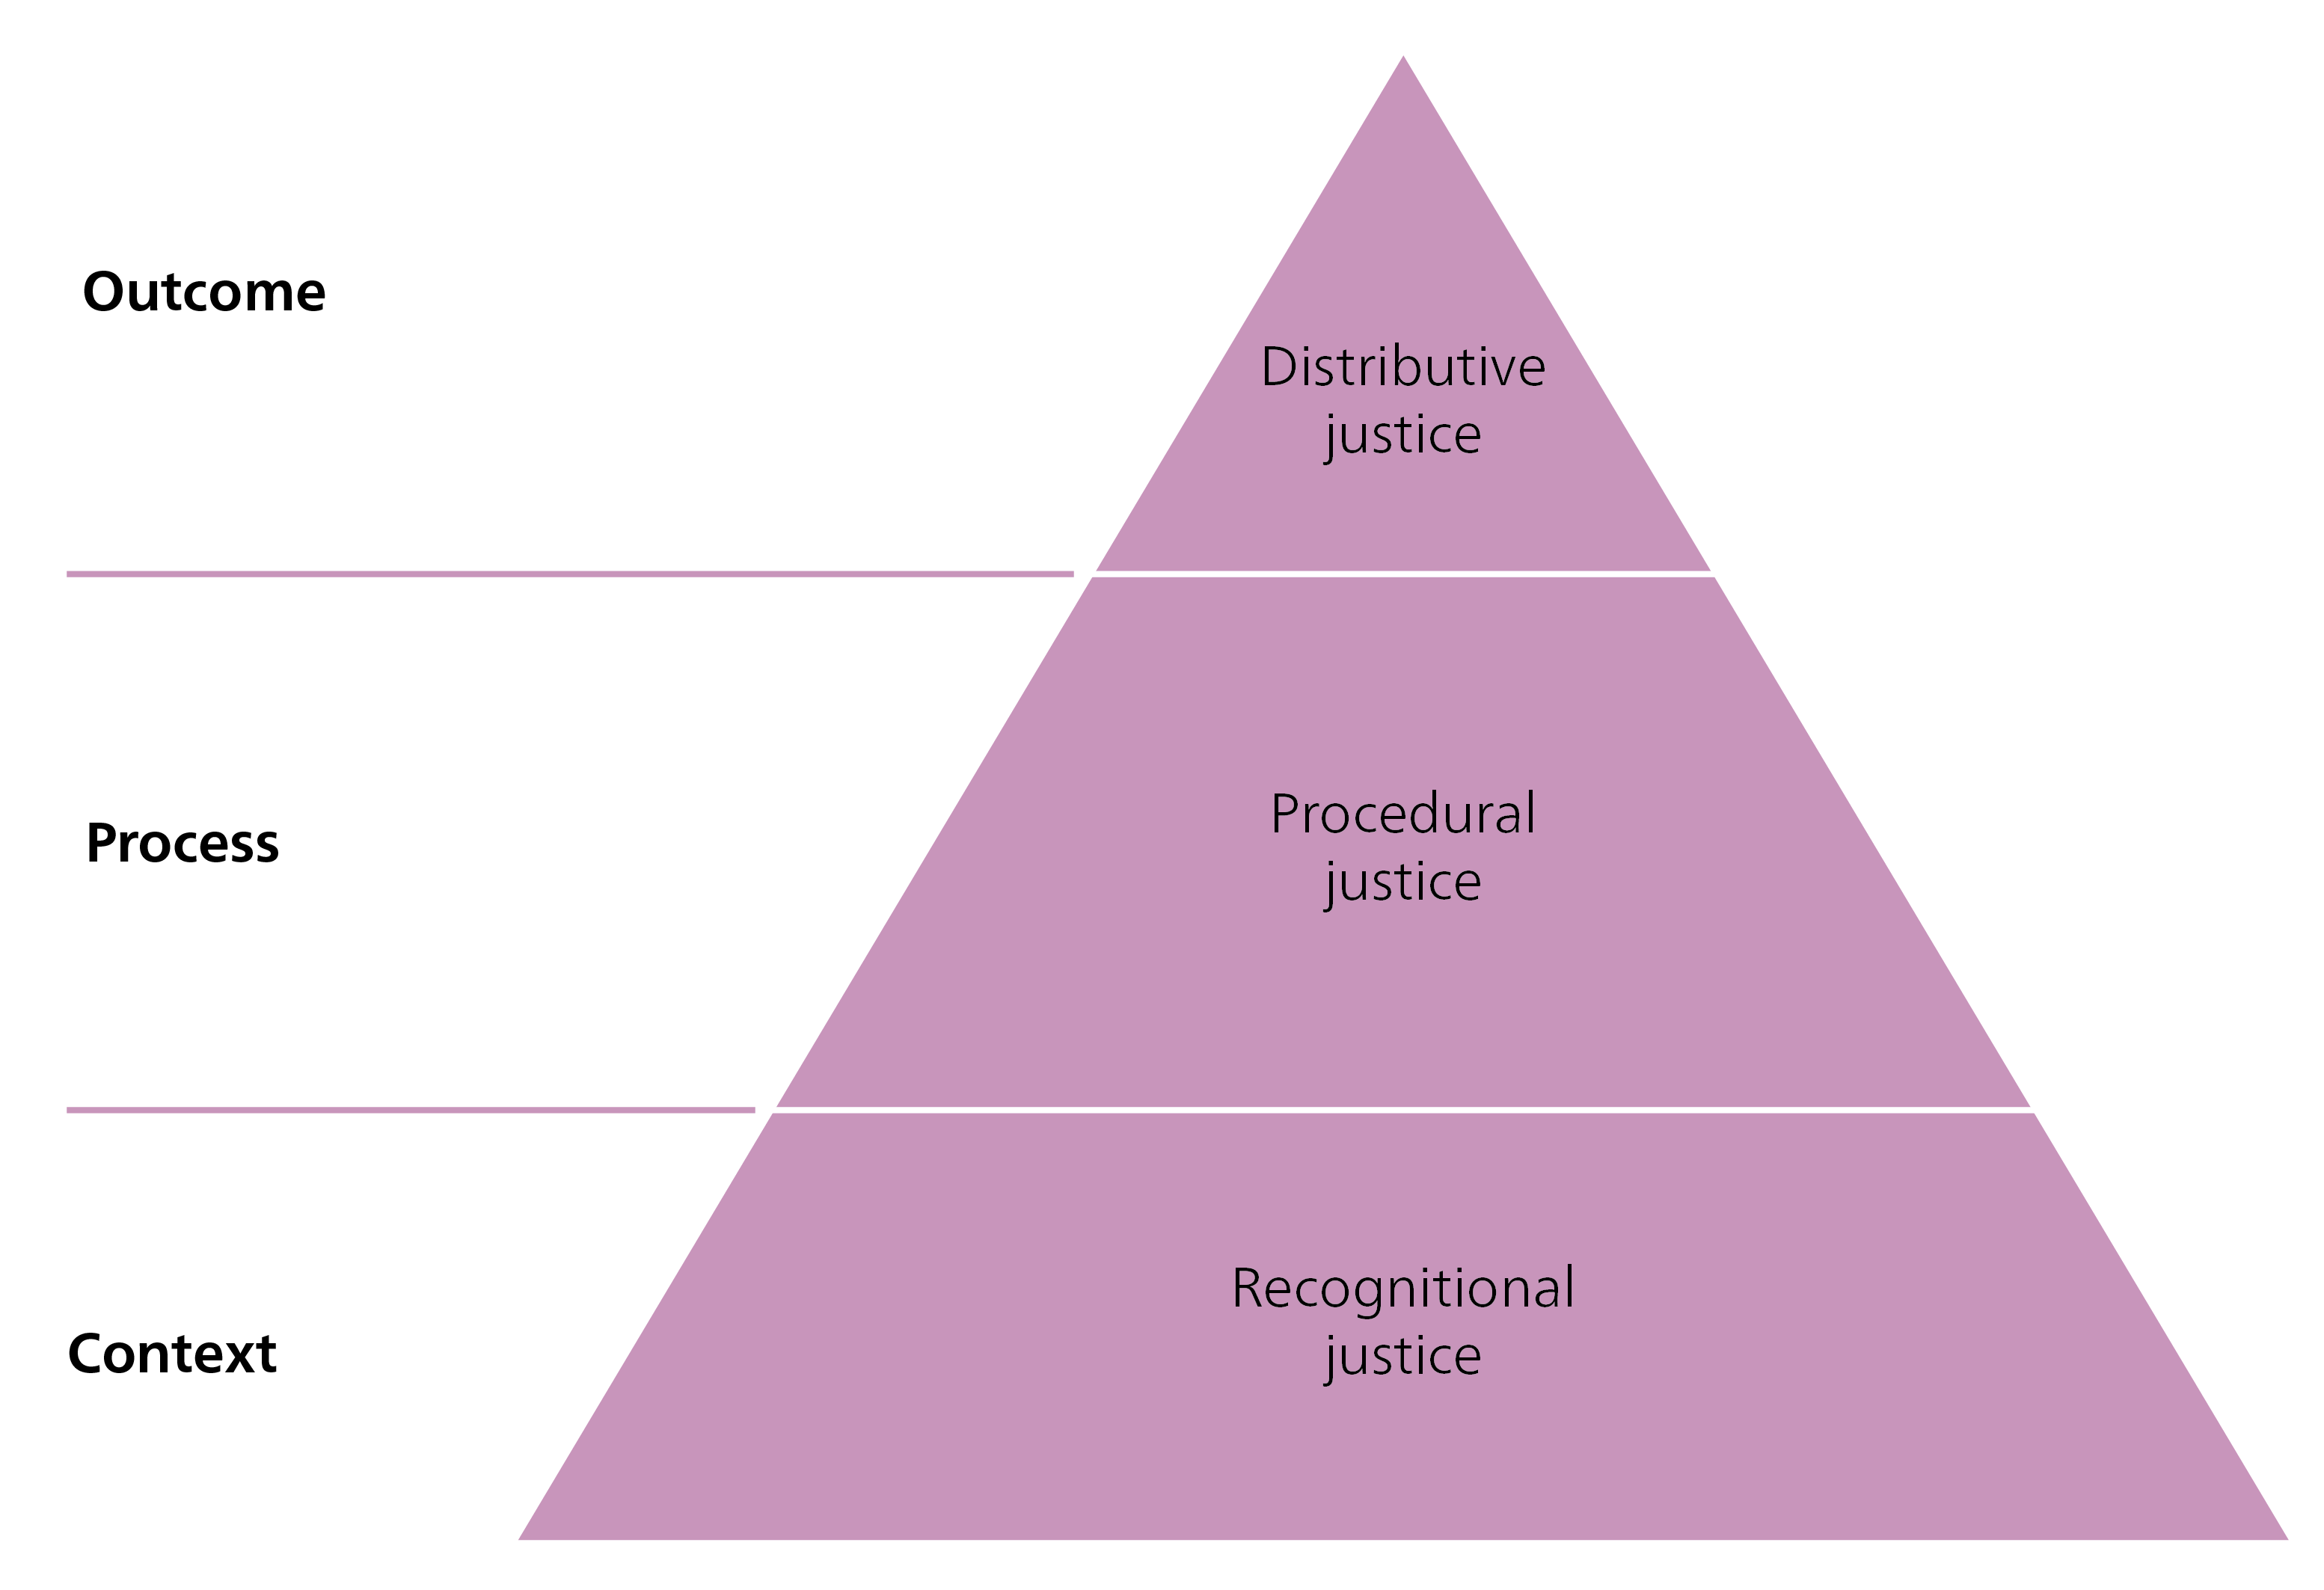
\includegraphics[keepaspectratio]{4_social-sustainability/images/Fig4_3_Justice.png}}

}

\caption{\label{fig-justice}The respective focus areas of distributive
justice, procedural justice, and recognition justice. Source: Own
illustration adapted from See \& Wilmsen (2022).}

\end{figure}%

\textbf{Distributive justice} is a results-oriented concept that aims at
a fair distribution of goods and burdens, regardless of social
differences. This principle applies to issues such as access to clean
water, the unequal burden of environmental pollution, or equal pay.

\textbf{Procedural justice} focuses on the inclusivity of
decision-making processes. It calls for underrepresented groups to be
fairly represented in institutions so that their perspectives can be
heard and incorporated into decision-making processes.

\textbf{Recognition justice} emphasizes the importance of the context,
and of respect for social and cultural differences. It involves
recognizing structural injustices, respecting the dignities and values
of different people and social groups, and understanding that diverse
needs and preferences are rooted in different historical experiences,
identities, and cultural backgrounds.

Table X shows how these three dimensions influence each other (Wijsman
\& Berbés-Blázquez, 2022). A more detailed discussion of distributive
and procedural justice follows in Section 3.2.6, as these are the
dimensions that most affect social sustainability debates.

\begin{longtable}[]{@{}
  >{\raggedright\arraybackslash}p{(\linewidth - 6\tabcolsep) * \real{0.2500}}
  >{\raggedright\arraybackslash}p{(\linewidth - 6\tabcolsep) * \real{0.2500}}
  >{\raggedright\arraybackslash}p{(\linewidth - 6\tabcolsep) * \real{0.2500}}
  >{\raggedright\arraybackslash}p{(\linewidth - 6\tabcolsep) * \real{0.2500}}@{}}
\toprule\noalign{}
\begin{minipage}[b]{\linewidth}\raggedright
\end{minipage} & \begin{minipage}[b]{\linewidth}\raggedright
Distributive justice
\end{minipage} & \begin{minipage}[b]{\linewidth}\raggedright
Procedural justice
\end{minipage} & \begin{minipage}[b]{\linewidth}\raggedright
Recognition justice
\end{minipage} \\
\midrule\noalign{}
\endhead
\bottomrule\noalign{}
\endlastfoot
\textbf{Distributive justice} & & The distribution of resources can
influence how easy or difficult it is for individuals or communities to
participate in decision-making processes. This is because participation
requires time, energy, and financial resources. & The distribution of
resources can influence whose interests are taken into account \\
\end{longtable}

in decision-making processes -- and whose identity is recognized and
considered important. \textbar{} \textbar{} \textbf{Procedural justice}
\textbar{} Participation in decision-making processes can have an impact
on their outcomes -- and therefore on how advantages and disadvantages
are distributed between individuals and groups. \textbar{} \textbar{}
Participation in decision-making processes can influence whose interests
are heard and which individuals or communities are recognized as
important. \textbar{} \textbar{} \textbf{Recognition justice} \textbar{}
Recognizing individuals or groups as valuable can influence how
resources are distributed. \textbar{} Recognizing individuals or groups
as valuable can also determine who is invited to participate in
decision-making processes. \textbar{} \textbar{}

\section{Defining social
sustainability}\label{defining-social-sustainability}

Over time, discussions on social sustainability have focused on
different issues. These include poverty reduction, development, basic
needs, livelihoods, and equity -- as well as identity, belonging, and
community stability and security (Glasson \& Wood, 2009). This thematic
diversity is reflected in the numerous available definitions of social
sustainability. Indeed, the literature is often described as fragmented,
vague, or at times chaotic (Mehan \& Soflaei, 2017). Some researchers
have even argued that the concept of social sustainability has changed
more than the environmental and economic dimensions over the past 30
years (Foladori, 2005).

Social sustainability can therefore best be understood as a dynamic
concept that takes different forms, depending on the time and place
(Boyer et al.~2016; Dempsey et al.~2011). Social priorities are diverse
and context-specific, and they change over time. In addition, there are
major cultural and local differences with regard to what is considered
socially justifiable and desirable.

Despite this diversity, definitions of social sustainability generally
describe a positive state that already exists or is considered
achievable. It is often associated with the goal of strengthening social
cohesion and providing basic services that contribute to well-being,
such as healthcare, education, mobility, housing, or leisure facilities.
Social sustainability is achieved when social processes, systems,
structures, and relationships actively support current and future
generations in creating healthy and viable communities.

For the Brundtland Commission (Our Common Future, 1987), the main goal
of the social dimension of sustainable development is to fulfil basic
human needs. These include not only clean water, food, and security --
they also extend to aspects such as well-being, justice, a democratic
system of government, and a vibrant civil society. This comprehensive
definition can be applied flexibly in different contexts.

In a bid to provide a more concrete framework, Barron et al.~(2023) and
Cuesta et al.~(2024) propose the following structured approach (see
Figure X).

\begin{figure}[H]

\centering{

\pandocbounded{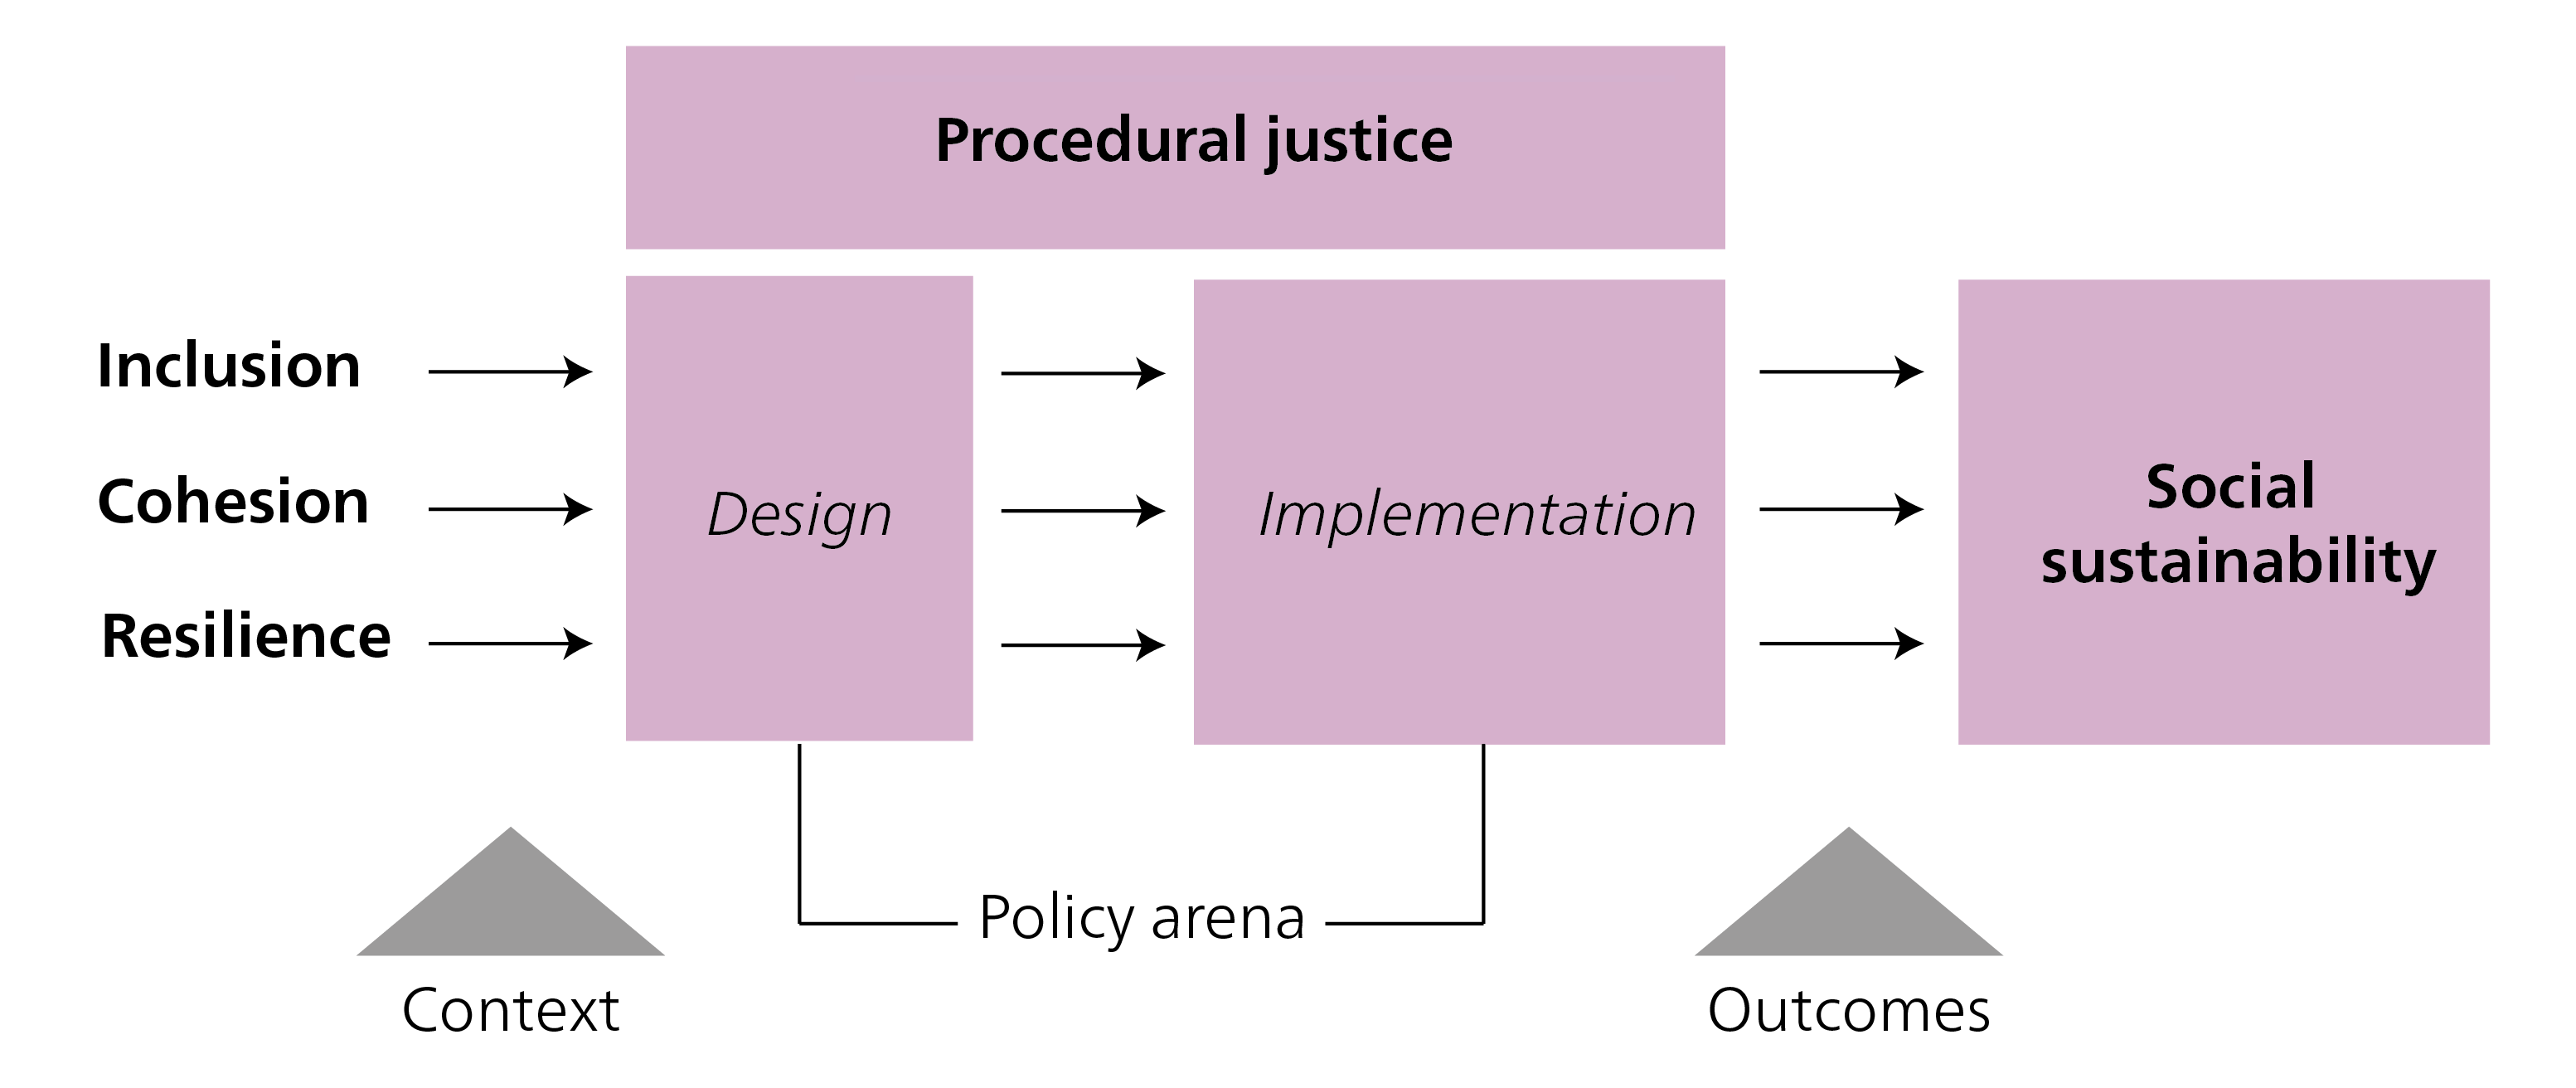
\includegraphics[keepaspectratio]{4_social-sustainability/images/Fig4_4_Framework.png}}

}

\caption{\label{fig-framework}A structured approach to social
sustainability. Adapted from Barron et al.~(2023, p.~31) \& Cuesta et
al.~(2024).}

\end{figure}%

The left-hand side of Figure X depicts three dimensions of a particular
context, namely: inclusion, social cohesion, and resilience. Each of
these dimensions -- defined below -- may be found in a community or
society to a greater or lesser extent:

\begin{enumerate}
\def\labelenumi{\arabic{enumi}.}
\item
  \textbf{Inclusion} refers to the access of all individuals and groups
  to the economic, political, social, and cultural spheres.
\item
  \textbf{Social cohesion} is a shared sense of belonging and trust that
  enables communities and groups to work together without conflict.
\item
  \textbf{Resilience} refers to the ability to avoid internal or
  external shocks -- such as environmental changes or political crises
  -- or to cushion their effects.
\end{enumerate}

The middle part emphasizes the importance of \textbf{procedural
justice}---the fairness of decision-making processes in the
\textbf{design} and \textbf{implementation} of policies and programs.
When these processes are perceived as fair, transparent, and
trustworthy, they generate \textbf{process legitimacy}, meaning that
people accept the authority of decisions and are more likely to support
and comply with them. The process of designing and implementing policies
and programs takes place within a so-called ``policy arena''. The term
``policy arena'' is broadly defined and encompasses political forums at
the local, national, regional, or global level, where resources are
allocated, goals are set, and decisions are made.

Finally, the right-hand side of the figure depicts the outcomes of the
design and implementation process. This process can foster -- but also
inhibit -- inclusion, social cohesion, and resilience. These outcomes,
in turn, influence the future level of social sustainability. In other
words, social sustainability exists when inclusion, social cohesion, and
resilience are gradually strengthened over time -- ideally in a
legitimate and transparent process.

The following sections explain the core elements of inclusion, social
cohesion, resilience, and justice (both procedural and distributive) in
more detail.

\section{Inclusion}\label{inclusion}

Inclusion addresses issues of social inequality. Social inclusion aims
at enabling all people to participate in society -- specifically, by
reducing deep-rooted systemic disadvantages. Many individuals and groups
face barriers that limit their socio-economic participation. While such
barriers may include poverty or having a low income, other forms of
discrimination and exclusion may be based on gender, age, origin,
occupation, ethnicity, religion, nationality, disability, sexual
orientation, or gender identity. Such inequalities are reinforced by
formal and informal norms, behaviour, laws, and institutions.

This raises normative questions: At what point is inequality considered
problematic? And what level of inequality is socially unacceptable?
Inclusion should not be understood as a form of charity, i.e.~as
something that is only ``right'' for ethical reasons. Reducing
inequalities has considerable benefits for all of society. Greater
inclusion and equal opportunities lead to better results in income,
poverty reduction, and human capital (OECD, 2015).

For example, a US study by Hsieh et al.~(2013) found that a reduction in
discrimination against female and Black workers accounted for 15 to 20\%
of economic growth per worker between 1960 and 2010. This growth was
attributed to an increase in talented people gaining access to better
opportunities. Other studies show that gender inequality can have a
negative impact on economic growth (Fabrizio et al.~2018; Klasen \&
Lamanna, 2009). There is also a link between inclusion and social
stability: countries that actively promote the political participation
and inclusion of disadvantaged groups tend to experience fewer social
conflicts (United Nations \& World Bank, 2018).

In short, the costs of social inequality -- such as fewer educational
opportunities, lower lifetime incomes, or poorer health (Buehren et
al.~2019; Wodon \& de la Briere, 2018) -- are not only ethical issues.
They also affect the overall economy, as they reduce potential, weaken
productivity, and increase the risk of conflict. By contrast, more
inclusive societies are more just, more stable, and more economically
efficient.

\subsection{(In)equality}\label{inequality}

As inequality is complex and diverse, there are different ways of
analysing, measuring, and evaluating it. This involves asking questions
about \emph{wh}o is affected and \emph{where} -- and in \emph{what}
fieldsinequalities occur (see Figure X; Sen, 1979).

\begin{figure}[H]

\centering{

\pandocbounded{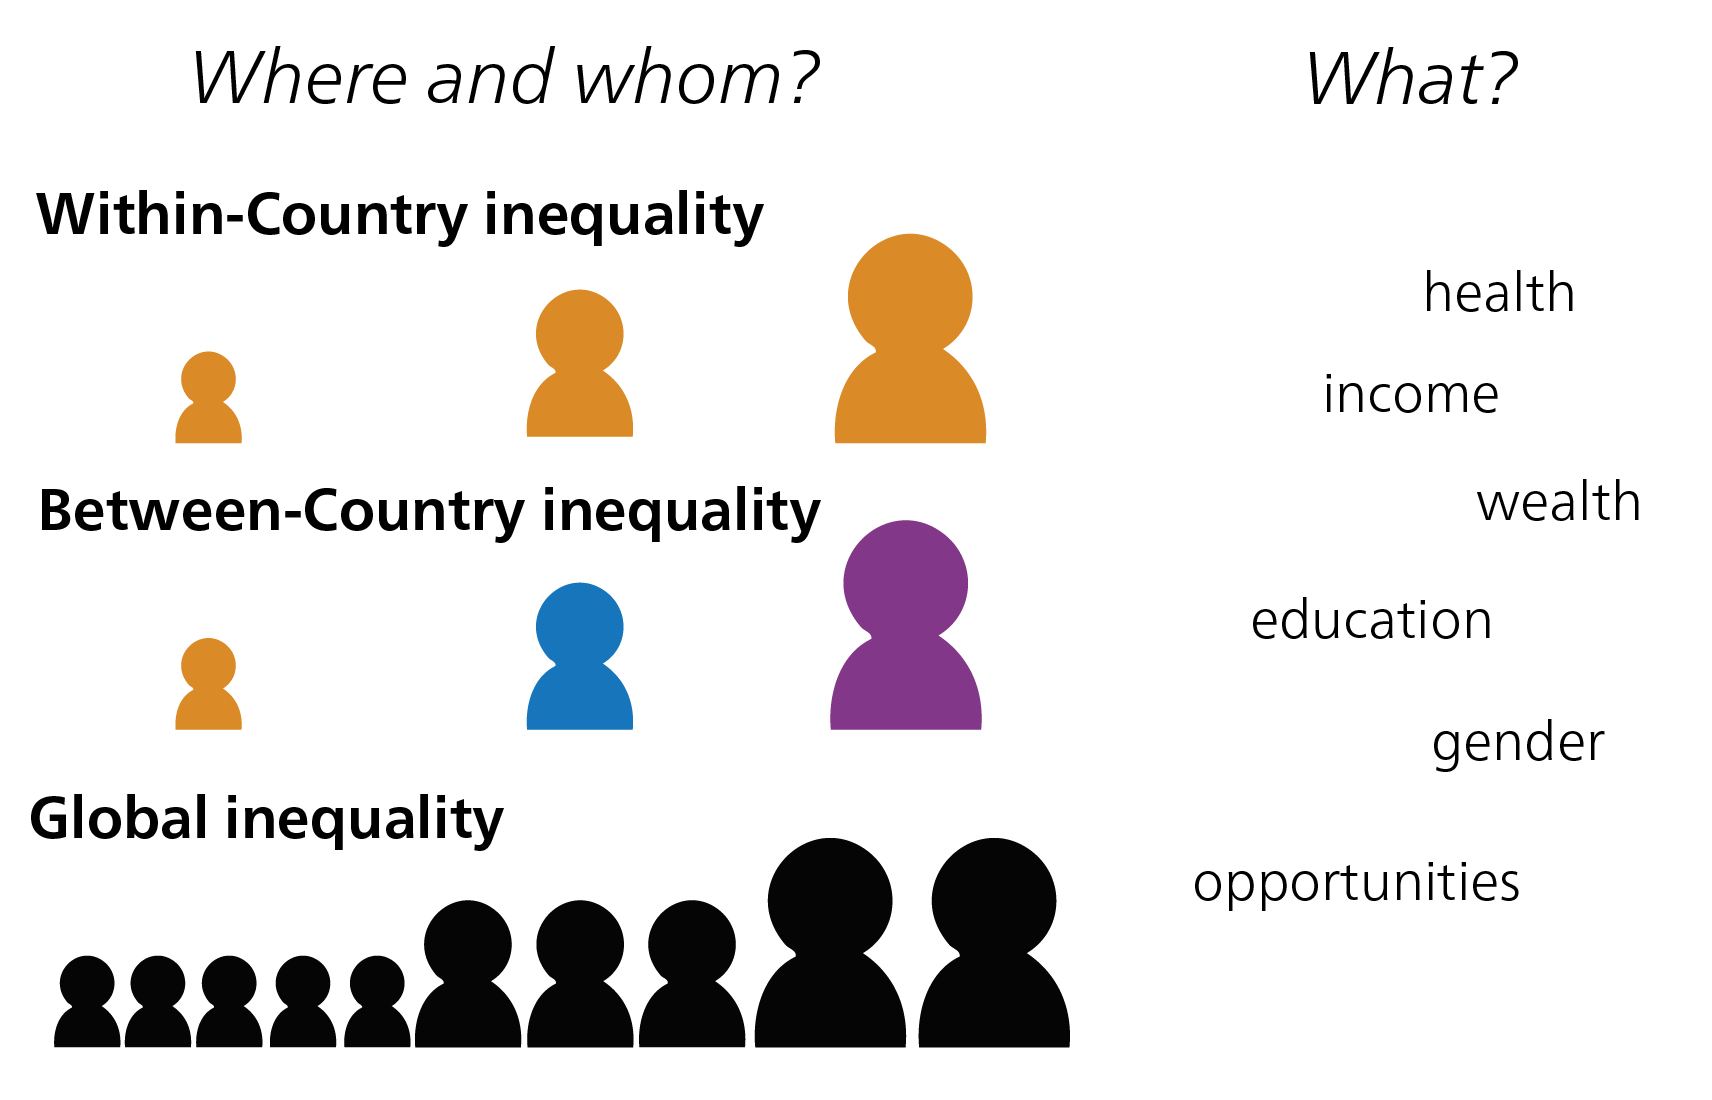
\includegraphics[keepaspectratio]{4_social-sustainability/images/Fig4_5_EqualityWhat.png}}

}

\caption{\label{fig-EqualityWhat}Equality of what? Source: Own
illustration based from Sen (1979)}

\end{figure}%

Inequality can be approached from various perspectives. Below, we
provide more detail on the aforementioned capability approach.

\textbf{Approaching inequality: Guided by Sen's question ``Equality of
what?'' - the capability approach}

The \textbf{capability approach} provides a normative framework for
assessing inequality and human well-being that goes beyond conventional
distribution principles. Traditional approaches to distributive justice
often aim either at ensuring equal distribution based on performance or
at guaranteeing a minimum level of resources for all. However, achieving
complete equality between individuals -- i.e.~\emph{equality of outcome}
-- is nearly impossible, as many influencing factors are distributed
randomly or unfairly. It is therefore considered fairer to focus on
\emph{equality of opportunity.} This principle aims to ensure that every
person has the chance to lead a meaningful and dignified life with
access to at least a minimum level of prosperity. This minimum level
should suffice to cover basic needs and guarantee equal civil rights,
ensuring that everyone has what they need to meet their needs and
participate equally in society.

Developed in the 1980s by the Indian economist, philosopher, and Nobel
Prize winner \textbf{Amartya Sen} and later expanded by the philosopher
\textbf{Martha Nussbaum}, the capability approach serves as an
alternative to traditional welfare economics, which measures prosperity
primarily through economic indicators (Roder, 2020). The capability
approach shifts attention away from formal entitlements or economic
aggregates toward people's \textbf{real freedoms to live the life they
value}. It emphasizes that genuine development depends not only on the
existence of opportunities and resources but also on whether individuals
can actually make use of them in practice. This, in turn, is shaped by
personal factors such as health or disability as well as by social,
political, and environmental conditions. For instance, for people with
disabilities, well-being requires more than the formal recognition of
rights; it depends on an inclusive society that removes barriers,
combats discrimination, ensures access to education, and enables
participation in political and social decision-making.

The capability approach defines well-being in terms of
\textbf{capabilities} and \textbf{functionings}. Capabilities are real
opportunities for action -- i.e.~what people could do or be if they were
free to choose. For example, being well-nourished, getting married,
being educated, or travelling without restrictions. Functionings are the
capabilities that are actually converted. Whether people can convert
available resources such as income, education, or public services into
functionings depends on \textbf{conversion factors}. These include
personal characteristics, social structures, and environmental
conditions. They ultimately determine whether capabilities and
functionings can actually be used.

The capability approach, therefore, shifts the focus from
\textbf{equality} to \textbf{equity}. While \emph{equality} aims to
ensure that everyone receives the same resources (i.e.~input),
\emph{equity} focuses on the result: what does a person need, to achieve
a comparable level of well-being (i.e.~output)? (see Figure X).

\begin{figure}[H]

\centering{

\pandocbounded{\includegraphics[keepaspectratio]{4_social-sustainability/images/Fig4_6_EqualityEquity.jpg}}

}

\caption{\label{fig-EqualityEquity}Equality vs.~equity. Source:
Reproduced with permission of the Robert Wood Johnson Foundation,
Princeton, N.J.}

\end{figure}%

\textbf{Approaching inequality: Where and whom?}

Building on the capability approach, which emphasizes people's real
opportunities to lead the lives they value, it is crucial to recognize
that inequality can manifest in different ways and be assessed across
various dimensions. Inequality can be analyzed in different spaces, for
example by distinguishing between \textbf{absolute} and \textbf{relative
inequality} (Niño-Zarazúa et al.~2017) or between \textbf{vertical} and
\textbf{horizontal} inequality (Stewart, 2005).

\textbf{Absolute inequality} describes a situation in which people are
unable to meet their most basic survival needs. This is the case, for
example, when a person does not have access to clean drinking water,
enough food, or safe housing, and lives below the poverty line. This
form of inequality is often defined by fixed income thresholds, such as
the World Bank's international poverty line.

\textbf{Relative inequality} measures a person's disadvantage in
relation to the average standard of living within a particular society
or community. For example, while a family in a rich country may have
enough income to cover food and housing, they may lack the resources to
participate fully in society -- if, say, they can't afford internet
access or their children's school trips. Relative inequality becomes
evident when living conditions fall significantly below the social
average. It often leads to social exclusion and limits access to
resources and the opportunities necessary to lead a dignified and
self-determined life in a particular social context. The key difference
between the two concepts is that \textbf{absolute poverty} refers to an
objective lack of essential goods, while \textbf{relative poverty}
describes a person's social and economic status in relation to others in
a society (Niño-Zarazúa et al.~2017).

Another concept distinguishes between \textbf{vertical} and
\textbf{horizontal inequality}. Vertical inequality focuses on
socio-economic differences between individuals -- such as in income,
occupational status, or education. By contrast, horizontal inequality
refers to differences between culturally defined groups, based for
example on gender, age, marital status, nationality, region, or place of
residence (Stewart, 2005).

\textbf{How to analyze inequality? Individual vs.~structural approaches}

Analyses of inequality often distinguish between \textbf{individual
inequality} and \textbf{structural inequality}. An analysis of
individual inequality draws on the principles of welfare economics and
the concept of absolute inequality. It focuses on socio-economic
characteristics such as differences in income, educational level, and
occupational status. This approach assumes that economic inequalities
are primarily the result of personal attributes and individual effort.

By contrast, analyses of structural inequality are more closely aligned
with the concepts of equity, the capability approach, and relative
inequality. Structural inequality is considered not as a product of an
individual's characteristics, but as a result of the social framework --
such as a person's position within the mode of production or the social
hierarchy; their access to wages, profits, or a pension; or their
nationality, all of which are key factors of global inequality (see
Milanovic, 2019).

This chapter has introduced various perspectives on inequality,
including the widely used capability approach, which offers an
overarching and normative perspective. The other perspectives may sound
similar, but in fact differ in their focus (see Table X).

\begin{longtable}[]{@{}
  >{\raggedright\arraybackslash}p{(\linewidth - 6\tabcolsep) * \real{0.0714}}
  >{\raggedright\arraybackslash}p{(\linewidth - 6\tabcolsep) * \real{0.3286}}
  >{\raggedright\arraybackslash}p{(\linewidth - 6\tabcolsep) * \real{0.2619}}
  >{\raggedright\arraybackslash}p{(\linewidth - 6\tabcolsep) * \real{0.3333}}@{}}
\toprule\noalign{}
\begin{minipage}[b]{\linewidth}\raggedright
\end{minipage} & \begin{minipage}[b]{\linewidth}\raggedright
relative vs.~absolute
\end{minipage} & \begin{minipage}[b]{\linewidth}\raggedright
vertical vs.~horizontal
\end{minipage} & \begin{minipage}[b]{\linewidth}\raggedright
individual vs.~structural
\end{minipage} \\
\midrule\noalign{}
\endhead
\bottomrule\noalign{}
\endlastfoot
\textbf{What is being compared?} & Inequality measured in relation to
differences vs.~absolute differences & Differences between income levels
vs.~differences between social groups & Differences due to personal
characteristics vs.~differences due to social structures \\
\textbf{Focus} & Categorization of inequality:

Who has more/less? & Categorization of inequality:

How is inequality quantified and represented? & Analysis dimension of
inequality:

What are the causes of inequality? \\
\textbf{Typical example} & The wealthy receive 40\% of the income, while
the poor receive 10\% (relative) vs.~the income gap required to meet
basic needs (absolute) & A CEO earns 100x more than a cleaner (vertical)
vs.~women earn less than men for the same work (horizontal) &
Individual: someone becomes successful through talent and effort
vs.~structural: someone is disadvantaged because of where they come
from \\
\textbf{Policy relevance} & Distributive justice vs.~combating poverty &
Redistribution vs.~anti-discrimination & Promotion of equal
opportunities vs.~reform of social structures \\
\end{longtable}

\section{Social cohesion}\label{social-cohesion}

\textbf{Social cohesion} describes the feeling of togetherness, trust,
and willingness to cooperate -- within groups, between different groups,
and towards state institutions. The concept describes the extent to
which people and communities act based on interpersonal and
institutional trust, what attitudes they have towards minorities, and
how secure they feel. Societies with strong social cohesion can be found
in wealthy countries and in countries affected by conflict alike (Cuesta
et al.~2024).

Functioning social cohesion and the well-being of a population require
that all social groups can participate economically, politically,
socially, and culturally. This is closely linked to inclusion and
inequality. However, rather than focusing on differences between
individuals or specific groups, the concept of social cohesion asks how
strongly the whole of society is connected.

Social cohesion is the foundation for mutual trust and collective
action. It is considered a core prerequisite for peace and prosperity
(Chatterjee et al.~2023). Studies show, for example, that societies with
a high level of trust experience less conflict (Putnam, 2000; Rothstein
\& Uslaner, 2005). By contrast, lower social trust is often associated
with greater economic inequality (Jordahl, 2007) (see Figure X).

\begin{figure}[H]

\centering{

\pandocbounded{\includegraphics[keepaspectratio]{4_social-sustainability/images/Fig4_7_TrustInequality.png}}

}

\caption{\label{fig-TrustInequality}Interpersonal trust vs.~income
inequality. Source: Our World in Data (2024).}

\end{figure}%

The above scatter diagram illustrates the relationship between
interpersonal trust and income inequality. Each dot represents a
country. Dot colour categorizes countries by their respective regions;
dot size reflects the country's population size. The Y-axis depicts the
percentage of a country's population that agrees with the statement
``Most people can be trusted''. The X-axis displays the Gini
coefficient, which is a widely used measure of income inequality: a
value of 0 indicates a state of complete income equality, while a value
of 1 (or 100\%) represents maximum income inequality -- i.e.~a single
person holding all the income, while everyone else receives none.

The graph shows that the level of social trust tends to be lower in
countries with a higher Gini index. One explanation for the negative
correlation between inequality and trust is that people tend to place
greater trust in those who are similar to them, and that greater
inequality leads to tensions and distributional conflicts (Alesina \& La
Ferrara, 2002). At the same time, some countries display low levels of
trust despite having a low Gini score (e.g.~Slovakia, Kyrgyzstan, and
Albania). This indicates that although a general trend is recognizable,
there is no causal relationship, and other factors are at play.

\textbf{Key elements of social cohesion}

Figure X is just one example of social cohesion. The concept is
difficult to define precisely, because the scientific literature varies
in regard to its exact meaning and how to measure it. Nevertheless, we
can identify three key elements (Schiefer \& van der Noll, 2017):

1. \textbf{Social relationships}: networks, trust, acceptance of
diversity, and participation

2. \textbf{Identification with society}: emotional attachment to the
social community

3. \textbf{Orientation towards the common good}: a sense of
responsibility, solidarity, and compliance with social rules.

Social cohesion is reflected in the attitudes and behaviour of all
social groups and encompasses both normative and relational dimensions.
It should be understood as a continuum along which societies can display
varying degrees of cohesion.

To illustrate how these elements are operationalized, it's worth looking
at how social cohesion is measured in Switzerland, where it has a
special significance: promoting ``internal cohesion'' is enshrined in
the Federal Constitution as an objective of the Swiss Confederation
(Art. 2). A crucial role in connecting people in multilingual
Switzerland is played by culture, which acts as ``societal cement''.
While social cohesion isn't an explicit goal in the 2030 Agenda, it's
implicitly addressed in several of its targets. In Switzerland, social
cohesion is defined and measured by the Federal Statistical Office,
using a range of indicators (see Table X; Federal Statistical Office,
2025).

The first element, \textbf{social relationships}, is reflected in
political participation such as voting. This element also involves
cultural participation, which is measured as the proportion of the
population that takes part in cultural activities. Social relationships
are negatively affected by factors such as discrimination, which
undermines the level of trust people place in fellow human beings and
institutions, as well as the sense of belonging to a social network.

The second element, \textbf{identification with society}, may be
reflected in how people perceive regional equality. In Switzerland, for
example, the Federal Statistical Office measures financial differences
between the cantons. Multilingualism is also relevant: The ability to
communicate with different language communities can strengthen one's
sense of belonging and promote intercultural understanding.

The third element, \textbf{orientation towards the common good},
encompasses aspects of social participation, particularly in the labour
market. This includes, for example, the employment rate of people with
disabilities or the unemployment rate according to migration status --
indicators of structural inclusion and solidarity. Social inequalities
are also key here, measured for example by the rate or risk of poverty
among the labour force. Another important indicator is civic engagement,
particularly through voluntary work, which is a direct measure of social
responsibility and public spirit.

\textbf{Education} is a cross-cutting issue, as it affects all three
elements: Education fosters social relationships, strengthens
identification with society, and supports an orientation towards the
common good by teaching about social norms and values. Relevant
indicators include the upper secondary completion rate and the
proportion of young people who are not in employment or education.

\begin{longtable}[]{@{}
  >{\raggedright\arraybackslash}p{(\linewidth - 2\tabcolsep) * \real{0.3381}}
  >{\raggedright\arraybackslash}p{(\linewidth - 2\tabcolsep) * \real{0.6619}}@{}}
\caption{Measuring social cohesion in Switzerland}\tabularnewline
\toprule\noalign{}
\begin{minipage}[b]{\linewidth}\raggedright
Key element (Schiefer \& van der Noll, 2017):
\end{minipage} & \begin{minipage}[b]{\linewidth}\raggedright
Indicators (Federal Statistical Office, 2025):
\end{minipage} \\
\midrule\noalign{}
\endfirsthead
\toprule\noalign{}
\begin{minipage}[b]{\linewidth}\raggedright
Key element (Schiefer \& van der Noll, 2017):
\end{minipage} & \begin{minipage}[b]{\linewidth}\raggedright
Indicators (Federal Statistical Office, 2025):
\end{minipage} \\
\midrule\noalign{}
\endhead
\bottomrule\noalign{}
\endlastfoot
Social relationships & \begin{minipage}[t]{\linewidth}\raggedright
\begin{itemize}
\item
  Political participation (e.g.~voting)
\item
  Cultural participation
\item
  Experience of discrimination
\end{itemize}
\end{minipage} \\
Identification with society &
\begin{minipage}[t]{\linewidth}\raggedright
\begin{itemize}
\item
  Regional differences (e.g.~financial capacity of cantons)
\item
  Multilingualism/cultural integration
\end{itemize}
\end{minipage} \\
Orientation towards the common good &
\begin{minipage}[t]{\linewidth}\raggedright
\begin{itemize}
\item
  Participation in the labour market (e.g.~employment rate of people
  with disabilities)
\item
  Social inequality (e.g.~poverty level)
\item
  Voluntary work
\end{itemize}
\end{minipage} \\
Cross-cutting issue & \begin{minipage}[t]{\linewidth}\raggedright
\begin{itemize}
\tightlist
\item
  Education
\end{itemize}
\end{minipage} \\
\end{longtable}

\section{Resilience}\label{resilience}

\textbf{Resilience} is the ability of individuals, households,
communities, or entire societies to prepare for, cope with, and recover
from shocks (Folke, 2016). Shocks can occur at an individual (e.g.~job
loss, illness) or societal level (e.g.~natural disasters, conflicts,
food shortages). They can occur suddenly (e.g.~natural disasters),
intensify gradually (e.g.~soil degradation), or be a constant presence
(e.g.~poverty, child labour, gender-based violence).

Societies with a high level of resilience can regain their quality of
life and economic stability more quickly after a shock. Resilience is
especially important for poor and marginalized groups, as they face more
shocks, suffer greater relative losses, and receive less support
(Bangalore et al.~201 7). Inequalities also mean that different groups
are unevenly or disproportionately affected by shocks (Hallegatte et
al.~2020). Depending on social norms, groups such as women, young
people, or the elderly are often more vulnerable or less adaptable
(Ajibade et al.~2013; Barrett et al.~2021).

We can identify three distinct strategies for addressing risk and
building resilience:

\begin{enumerate}
\def\labelenumi{\arabic{enumi}.}
\item
  \textbf{Risk reduction and mitigation}: Measures that reduce the
  likelihood of shocks or their negative consequences (Obrist et
  al.~2010). Examples include immunization, income diversification,
  local protection infrastructure, or state social systems.
\item
  \textbf{Coping strategies}: Responses to shock (Imperiale \& Vanclay,
  2021; Severi et al.~2012). Coping strategies include insurance models,
  recourse to savings or loans, and support from social networks.
  Governments can also help, for example through cash transfers or
  social programmes. However, without sufficient resources, people
  affected by shocks may resort to harmful, short-term measures, such as
  restricting essential consumption, overexploiting resources, or using
  child labour.
\item
  \textbf{Transformative strategies}: Far-reaching reforms or new
  institutions that increase the long-term resilience of societies
  (Mozumder et al.~2018; Pfefferbaum et al.~2017), typically combining
  risk reduction and coping strategies. For example, establishing a
  government agency for flood preparedness that improves early warning
  systems, fosters risk reduction research, and develops flood response
  plans. Or introducing measures to reduce the risk of gender-based
  violence by investing in legal, institutional, and awareness-raising
  programmes that change incentives and social norms regarding violence.
\end{enumerate}

\subsection{Basic needs as a prerequisite for
resilience}\label{basic-needs-as-a-prerequisite-for-resilience}

In the aforementioned doughnut economics framework, resilience is only
possible if all people can meet their basic needs. Meeting these social
foundations ensures that individuals and societies are better able to
cope with shocks. However, in countries of the Global South, these basic
needs are often unmet. Conversely, while wealthier countries are able to
meet these needs, they usually exceed planetary boundaries in doing so.
See Figure X comparing Switzerland and Laos (see Section 3.2.1).

\begin{figure}[H]

\begin{minipage}{0.50\linewidth}

\centering{

\pandocbounded{\includegraphics[keepaspectratio]{4_social-sustainability/images/Fig4_8_DoughnutA.png}}

}

\subcaption{\label{fig-Switzerland}Switzerland}

\end{minipage}%
%
\begin{minipage}{0.50\linewidth}

\centering{

\pandocbounded{\includegraphics[keepaspectratio]{4_social-sustainability/images/Fig4_8_DoughnutB.png}}

}

\subcaption{\label{fig-laos}Laos}

\end{minipage}%

\caption{\label{fig-elephants}Doughnut visualization for Switzerland
(left) and Lao PDR (right), comparing each country's performance
relative to its social foundation and ecological ceiling. The green
doughnut represents the safe and just space where both ecological and
social boundaries are respected. Red areas indicate the magnitude of
ecological overshoot or shortfalls in meeting social needs, showing
where each country exceeds ecological limits or falls below minimum
social thresholds. Source: Kate Raworth and Christian Guthier. CC-BY-SA
4.0, https://doughnut-economy-fxs7576.netlify.app/}

\end{figure}%

These minimum social standards -- the ``social floor'' -- include access
to food, health, education, income, and work. They also include peace,
justice, political participation, social and gender equality, housing,
social networks, energy, and water. In this textbook, we use the example
of \textbf{food} to show how access to one of these standards affects
resilience. Difficulties with a single standard rarely occur in
isolation and often affect other areas as well. Ensuring these social
foundations is therefore crucial to sustainable development.

\textbf{Global food security}

Food security means having enough food and reliable access to it,
especially staple foods. A household is considered food secure when its
members are not at risk of hunger or malnutrition. Malnutrition has
severe health impacts, such as emaciation and stunted growth. It also
increases healthcare costs, reduces productivity, and inhibits economic
growth, thereby reinforcing a cycle of poverty and disease.

Food security is closely linked to a food system's resilience -- its
ability to tolerate and adapt to change. Our global food system is
particularly vulnerable due to its complexity and the many
interdependencies among its elements. It is exposed to both external
threats -- such as the consequences of climate change -- and internal
risks, such as policy failures, unsustainable consumption patterns, or
market failures.

Figure X shows that almost 2.4 billion people worldwide were affected by
food insecurity in 2022. Just under half of these (1.1 billion) lived in
Asia, 37 per cent (868 million) in Africa, 10.5 per cent (248 million)
in Latin America and the Caribbean, and around 4 per cent (90 million)
in North America and Europe. The figure also shows the proportions of
severe and moderate food insecurity: severe food insecurity means that
people have difficulty meeting their short-term basic food needs.
Moderate food insecurity, on the other hand, refers to an inadequate
supply of essential nutrients, which can result in health problems.

\begin{figure}[H]

\centering{

\pandocbounded{\includegraphics[keepaspectratio]{4_social-sustainability/images/Fig4_9_FoodInsecurity.png}}

}

\caption{\label{fig-FoodInsecurity}The concentration and distribution of
food insecurity by severity differ greatly across the regions of the
world. Source: FAO et al.~(2023). FAOSTAT: Suite of Food Security
Indicators, www.fao.org/faostat/en/\#data/FS}

\end{figure}%

This demonstrates the need for fair and resilient food systems. As
Figure X shows, a food system encompasses all activities, actors, and
infrastructures involved in the production, processing, transport,
distribution, trade, consumption, and disposal of food. Food systems are
deeply embedded in society and the environment. Changes within these
systems therefore affect numerous areas: the environment (water, air,
soil, biodiversity), social and cultural aspects (e.g.~impact on local
communities), the economy (value chains, trade, financing), and health
(Tribaldos \& Kortetmäki, 2022).

Discussions on combating food insecurity often focus on increasing
yields and reducing food waste, but these approaches are not proving to
be the most effective. Current food production and consumption habits
increasingly rely on highly processed meat and dairy products, as well
as intensive production methods. Global consumption leads to outsourced
environmental impacts like soil degradation, biodiversity loss, water
overuse, and the disappearance of local plant varieties -- impacts that
primarily affect the producers, not the consumers.

Focusing solely on increasing production also overlooks the fact that
the world already produces enough food. What's needed instead is a
far-reaching transformation in how these resources are used and
distributed. For example, Shepon et al.~(2018) found that plant-based
substitutes that are nutritionally comparable (e.g.~in terms of protein
content) are significantly more efficient than animal products: On one
hectare of arable land, up to 20 times more food can be produced than
with beef and twice as much as with eggs, which represent the most and
least resource-intensive animal foods, respectively.

However, the current food system feeds large quantities of edible crops
to farm animals. According to Berners-Lee et al.~(2018), around 41\% of
human-edible crops (measured by kilocalories per person per day) are fed
to farm animals. This process is highly inefficient: the animals only
return around 12\% of that energy in the form of meat, fish, and dairy
products. In other words, a significant proportion of potential food for
human consumption is lost in the process (see Figure X).

\begin{figure}[H]

\centering{

\pandocbounded{\includegraphics[keepaspectratio]{4_social-sustainability/images/Fig4_10_GLobalFoodSupply.png}}

}

\caption{\label{fig-GlobalFood}The flows of global food energy
(kcal/person/day) show the path from the food produced to the food
actually consumed in 2013. For crops fed to animals, the units are based
on the world population, not the animal population. The left-hand bar
distinguishes between crops that are directly edible for humans and
fodder crops such as grass, pasture, or crop residues that can only be
used by animals. Animal losses (grey bar) include all energy losses that
occur in animal husbandry, for example through respiration, growth,
movement, and reproduction, as well as through animal components that
are not used as food. The outermost right-hand bar divides the nutrients
consumed into the proportion required for a healthy human life,
i.e.~showing a small net increase in food consumption in 2014. Source:
(Berners-Lee et al.~2018) licensed under Creative Commons CC BY.}

\end{figure}%

\section{Justice}\label{justice}

\subsection{Procedural Justice}\label{procedural-justice}

\textbf{Inclusion, social cohesion, and resilience} are considered the
three key dimensions of social sustainability. However, whether these
factors actually enable social sustainability depends on a fourth
element: \textbf{procedural justice}. Procedural justice is decisive in
determining whether, and to what extent, social change succeeds across
the three dimensions.

Procedural justice focuses on the process. It describes \emph{how}
policies are developed, programmes designed, and measures implemented. A
high degree of procedural justice is achieved when decision-making
processes are perceived as fair, trustworthy, and aligned with social
norms (Hinsch, 2016; Wijsman \& Berbés-Blázquez, 2022), even when
addressing conflicts and tensions. This is not an either/or situation,
but rather a continuum: processes can be perceived as more legitimate or
less legitimate, and different groups often perceive this differently.

Ensuring legitimacy requires the public perception that decisions are
made by trustworthy and recognized actors who act in accordance with
shared values and agreed rules. Legitimacy is further strengthened
through transparency, participation, and tangible benefits for those
affected. This is particularly relevant when decisions entail costs or
burdens for certain groups, such as land redistribution, carbon taxes,
or changes in working conditions. How procedural justice is achieved
largely depends on the respective societal context, culture, and
structures. In general, however, we can identify five key drivers:

\begin{enumerate}
\def\labelenumi{\arabic{enumi}.}
\item
  \textbf{Ensuring credibility of decision-makers:} Legitimacy increases
  when authority stems from recognized sources such as elections,
  expertise, or institutional confirmation.
\item
  \textbf{Adhering to agreed rules:} Processes are considered legitimate
  if they are based on accepted standards, procedures, or traditions.
\item
  \textbf{Conforming with societal values:} The process takes into
  account moral, religious, or philosophical beliefs.
\item
  \textbf{Demonstrating perceived benefits:} Legitimacy increases when
  the affected parties believe they will benefit from the decisions.
\item
  \textbf{Promoting participation and transparency:} Open dialogue and
  co-creation foster acceptance, especially in the event of conflicts.
\end{enumerate}

These drivers often interact and reinforce each other, with the relative
importance of each driver depending on the social context. As shown in
Figure X (Section 3.2.2), procedural justice encompasses both the design
and the implementation of policies, programmes, and initiatives. These
processes take place within a \textbf{policy arena}, the term used to
describe all constellations in which policies and programmes are
formulated and implemented, such as parliaments, ministries, companies,
associations, or local initiatives. However, the policy arena is
becoming increasingly fragmented and polarized, amid challenges like
social media and disinformation. This weakens the credibility of
information and hinders the ability to build broad consensus and
legitimacy in decision-making processes.

In Switzerland, this is exemplified by political representation, which
fails to adequately reflect the composition of the population: An
analysis of the 2023 elections shows that women hold only 37.8\% of
seats in the National Council. Non-binary people are not yet included in
statistics on political representation. In addition, the Swiss
parliament is considered a ``club of the highly educated'', as the
proportion of councillors with a university degree is twice as high as
in the general population. Only around one in six (or 16\%) of the
candidates had a ``migration background'' -- compared to around 40\% of
the population. A quarter of the adults living in Switzerland do not
have the right to vote.

Political scientist Joachim Blatter describes this exclusion from
political participation as a ``\textbf{democratic deficit}'', noting
that Switzerland excludes more people from the political system than
most other European countries (Blatter et al.~2017). In some
municipalities, where only a fraction of the population is entitled to
vote, this can mean that ultimately that only 10--20\% of residents have
a say in political decisions (Debelle, 2020).

\subsection{Distributive justice}\label{distributive-justice}

As described in Section 3.2.1.1, the various dimensions of justice
influence one another. While \textbf{procedural justice} focuses on the
process, \textbf{distributive justice} concentrates on the outcome of
the process. Distributive justice could involve ensuring the fair
distribution of environmental resources and environmental impacts.
Measures that aim at distributive justice include progressive taxation,
social safety nets (e.g.~old-age and unemployment insurance), and
enforcement of equal pay regardless of gender, ethnicity, or other
discriminatory factors.

Historically, discussions about distributive justice were primarily
limited to political communities, such as national governments, and
focused solely on the current generation. However, sustainability issues
require a broader perspective. Distributive justice must be considered
globally and intergenerationally, as well as in relation to our
responsibility towards the environment and other affected species.
Climate targets are a case in point: how should emissions reduction
targets be distributed between countries, between generations, or
between different social groups? Who should bear the costs of adapting
to climate change?

Thus, distributive justice encompasses a wide range of topics. Take the
issue of income, for example. In Switzerland, women earn on average CHF
1,364 less per month than men, despite the principle of ``equal pay for
work of equal value'' being enshrined in the Federal Constitution since
1981. Around half of this difference can be explained by objective
factors such as education or sector, but the other half -- which is as
of yet unexplained -- could indicate wage discrimination (EBG, 2023).
The principle is widely accepted and rarely disputed. Consequently,
opponents of measures to implement equal pay tend not to take issue with
the principle itself, attempting instead to justify the gap by citing
allegedly objective factors.

However, social consensus is far harder to achieve in other questions of
distributive justice. Various theories (see Box X) and concepts (see Box
X) seek to answer the question of ``What is fair?''. They offer
different perspectives on what individuals or groups perceive as fair,
and provide guidance on how social advantages and disadvantages should
be distributed. A controversial example is that of \textbf{unconditional
basic income}. From a distributive justice perspective, this concept
could be considered fair, as it distributes resources equally and
equalizes social opportunities. However, some argue that such a model
could weaken incentives to work and thus impair productivity and
innovation. Depending on the theory applied (see Box X), very different
conclusions can be drawn on such topics -- as shown in the reflections
after Box x.

\begin{tcolorbox}[enhanced jigsaw, left=2mm, arc=.35mm, titlerule=0mm, opacityback=0, leftrule=.75mm, title={Note \ref*{tip-justice}: Theories of justice}, breakable, bottomtitle=1mm, rightrule=.15mm, coltitle=black, toptitle=1mm, bottomrule=.15mm, colback=white, opacitybacktitle=0.6, colbacktitle=quarto-callout-note-color!10!white, toprule=.15mm, colframe=quarto-callout-note-color-frame]

\quartocallouttip{tip-justice} 

\textbf{Theories of justice} describe fundamental, overarching ideas
about how social structures and processes should be organized. They are
therefore considered one level above concepts of justice (Box X),
representing philosophically developed models that define, justify, and
explain the essence of justice.

\textbf{Libertarian theories} champion individual freedom and the right
to property. Adherents believe the state's role should be minimal, often
described as a \emph{night watchman state}.

\begin{itemize}
\item
  In \emph{Anarchy, State, and Utopia} (1974), \textbf{Robert Nozick}
  develops the idea of the minimal state, one that assumes only basic
  protective functions such as security and contract enforcement. Nozick
  rejects any further redistribution (e.g.~via taxes to fund welfare
  states) as an \emph{encroachment on individual freedom and property
  rights.}
\item
  In \emph{The Illusion of Social Justice} (1981), \textbf{Friedrich
  August von Hayek} argues that ``social justice'' is an empty term, and
  that no objective distributive justice is possible in complex market
  societies. Instead, the market should determine the allocation of
  resources through free pricing, as state intervention would inevitably
  lead to a loss of freedom.
\end{itemize}

\textbf{Liberal theories} also analyse societies based on individual
rights and property, but they do not recognize a ``natural'' right to
property. Unlike libertarianism, they do not necessarily view the free
market as the optimal means of fair distribution and assign an active
role to the state in redistribution.

\begin{itemize}
\item
  \textbf{Utilitarianism}: What is considered just is that which
  maximizes happiness (utility) and minimizes suffering, thereby
  creating the greatest possible long-term benefit for all parties
  involved.
\item
  \textbf{Contractarianism}: In \emph{A Theory of Justice} (1971), John
  Rawls uses a social contract thought experiment to determine fair
  principles for society. His two core principles are:

  \begin{enumerate}
  \def\labelenumi{\arabic{enumi}.}
  \item
    Equal right to basic freedoms: Each person is entitled to the most
    comprehensive system of equal fundamental freedoms that is
    compatible with a similar system for everyone else.
  \item
    Just social and economic inequalities: Inequalities are only
    considered just if they meet two conditions: they benefit the least
    advantaged in society (``the difference principle''), and offices
    and positions are open to all under conditions of fair equality of
    opportunity.
  \end{enumerate}
\item
  \textbf{Egalitarianism}: The aim is equal treatment for all, as
  everyone is equal in terms of dignity and moral status. One prominent
  approach is the capability approach (see Sections 3.2.1 and 3.2.3).
  \textbf{Ronald Dworkin} offered another key approach, formulating the
  theory of resource equality in \emph{What is Equality}? (1981).
  Dworkin posited that a society is just if resources are distributed in
  such a way that no redistribution would allow for a more equal
  distribution. The goal is not to achieve equal life satisfaction or
  equal prosperity, but to ensure fair starting conditions that enable
  individuals to pursue their own life plans.
\end{itemize}

\textbf{Collective theories} view societies as associations of social
groups or classes that differ in their relationships to means of
production and resources. They reject universalistic, abstract
principles, arguing instead that each community is the product of
specific historical and cultural conditions. Therefore, there are no
universal norms of justice; instead, context-dependent rules emerge that
are derived from social practices and traditions. Justice is understood
here in terms of the common good: What is socially just is what
strengthens a community's cohesion and continued existence.

\begin{itemize}
\item
  According to \textbf{Michael Walzer,} the given context leads to
  different ``spheres of justice''. What is considered just therefore
  varies according to time and place. In addition, different social
  goods warrant different criteria. In other words, political power
  should not be distributed according to the same standards as economic
  resources.
\item
  \textbf{Michael Sandel} emphasizes the importance of community and
  moral responsibility. For Sandel, justice and the common good are
  inextricably linked to belonging to a community that creates identity.
\end{itemize}

\end{tcolorbox}

When reflecting on the introduction of an unconditional basic income,
proponents of the various theories would arrive at very different
conclusions -- as shown in Table X.

\begin{longtable}[]{@{}
  >{\raggedright\arraybackslash}p{(\linewidth - 4\tabcolsep) * \real{0.3333}}
  >{\raggedright\arraybackslash}p{(\linewidth - 4\tabcolsep) * \real{0.3333}}
  >{\raggedright\arraybackslash}p{(\linewidth - 4\tabcolsep) * \real{0.3333}}@{}}
\caption{Evaluation of the introduction of an unconditional basic
income, based on various theories of justice}\tabularnewline
\toprule\noalign{}
\begin{minipage}[b]{\linewidth}\raggedright
Theories of justice
\end{minipage} & \begin{minipage}[b]{\linewidth}\raggedright
Is the idea of a basic income a good idea
\end{minipage} & \begin{minipage}[b]{\linewidth}\raggedright
Reasoning
\end{minipage} \\
\midrule\noalign{}
\endfirsthead
\toprule\noalign{}
\begin{minipage}[b]{\linewidth}\raggedright
Theories of justice
\end{minipage} & \begin{minipage}[b]{\linewidth}\raggedright
Is the idea of a basic income a good idea
\end{minipage} & \begin{minipage}[b]{\linewidth}\raggedright
Reasoning
\end{minipage} \\
\midrule\noalign{}
\endhead
\bottomrule\noalign{}
\endlastfoot
Libertarian theories (Nozick, Hayek) & No & Social justice cannot be
controlled centrally. The state should only assume minimal protective
functions, and resources should be allocated via the market.
Redistribution through taxes to finance a basic income is an
encroachment on individual freedom and property rights. \\
Liberal theories (Utilitarianism, Contractarianism, Egalitarianism) &
Yes/Maybe & From a utilitarian perspective, a basic income could
increase overall utility (or benefit). Contractarianism (Rawls) also
supports it, arguing that it strengthens equal basic freedoms. From an
egalitarian perspective, a basic income can promote opportunities, but
it is viewed critically because it emphasizes \emph{equality} (i.e.~that
everyone receives the same) rather than justice in the sense of
\emph{equity} (i.e.~that each person receives what they need).
Additional measures would be necessary to ensure equity. \\
Collective theories of justice (Walzer, Sandel) & Depends on context &
How this question is assessed depends on specific historical, cultural,
and social conditions. A basic income could be considered socially just
if it strengthens social cohesion and the common good. \\
\end{longtable}

While \textbf{theories of justice} are general frameworks or models that
define what justice is and how it can be achieved in a society,
\textbf{concepts of justice} focus more on specific aspects. As the
overview in Box X shows, distributive justice issues can be viewed from
a variety of different perspectives.

\begin{tcolorbox}[enhanced jigsaw, left=2mm, arc=.35mm, titlerule=0mm, opacityback=0, leftrule=.75mm, title={Note \ref*{tip-concepts}: Normative concepts of justice based on (Novy et al.~2023)}, breakable, bottomtitle=1mm, rightrule=.15mm, coltitle=black, toptitle=1mm, bottomrule=.15mm, colback=white, opacitybacktitle=0.6, colbacktitle=quarto-callout-note-color!10!white, toprule=.15mm, colframe=quarto-callout-note-color-frame]

\quartocallouttip{tip-concepts} 

\textbf{Market justice} is based on the principle of supply and demand,
meaning that income, goods, and opportunities are distributed according
to market mechanisms. According to this framework, the price determines
what is considered fair. Within neoclassical economic theory, market
justice is measured by the marginal productivity of labour, i.e.~how
work contributes to maximizing profit.

\textbf{Commensurability with performance} demands that remuneration be
proportionate to an individual's contribution. Since people perform to
different levels, unequal pay is considered justified. The problem is
that this principle fails to recognize key services -- such as care work
in the family -- that aren't valued on the market. Because performance
is difficult to measure, this principle is often equated with market
justice.\hyperref[_msocom_1]{{[}TH1{]}}~

\textbf{Equality of opportunity} aims to create equal starting
conditions -- i.e.~without legal and cultural discrimination or barriers
to market access -- for example through anti-discrimination laws that
prohibit discrimination based on gender, ethnicity, or religion.

\textbf{Equality of needs} ensures that basic needs are met -- such as
food, housing, or protection from poverty. It is aimed particularly at
people whose needs cannot be met through market mechanisms. While
commensurability with performance focuses on individual contributions,
equality of needs is about the collective provision of basic needs.

\textbf{Equality of participation} expands on the concept of equality of
needs and opportunities. It seeks to create equal opportunities to
participate in and help shape social life -- regardless of income. This
includes access to education, health, work, culture, and political
participation. Participation is seen as a prerequisite for achieving
other basic needs such as health and autonomy.

\textbf{Gender equality} addresses the unequal starting and
participation conditions that exist between genders. For example, to
promote equality of opportunity, quotas are a way of redressing
structural disadvantages for women. And to foster participatory justice,
policies that create affordable childcare or care services can help
alleviate the unequal burden of care work that disproportionately
affects women.

\textbf{Environmental justice} emphasizes the fair distribution of
environmental burdens and resources, as well as equal participation in
environmental policy decisions. The term originated in the US as a
response to the disproportionate placement of landfills and motorways
near poor African-American neighbourhoods. The US Environmental
Protection Agency (US EPA, 2015) defines environmental justice as the
fair treatment and effective participation of all people -- regardless
of race, colour, gender, or income -- in the design, implementation, and
enforcement of environmental laws and policies.

\textbf{Inter- and intragenerational equity} are defined in the
Brundtland Report (1987). Intergenerational equity refers to the balance
between present and future generations, while intragenerational equity
refers to the balance between the Global North and South. Both concepts
emphasize that opportunities for participation must be balanced across
time and space.

\textbf{Climate justice} is a specific form of environmental justice. It
addresses the unequal consequences of climate change for marginalized
and vulnerable groups, and seeks to promote the fair distribution of
burdens and measures aimed at reducing emissions. The Paris Climate
Agreement stipulates that both the Global North and South must share
responsibility for reducing CO₂ emissions. However, the North bears a
greater obligation due to historically higher emissions -- and must
therefore reduce its emissions faster than countries in Africa, Latin
America, or Asia.\\
\strut \\

~\hyperref[_msoanchor_1]{{[}TH1{]}}Not really sure what this means? Can
you clarify?\\
\strut \\

Weil Leistung schwer messbar ist, wird Leistungsgerechtigkeit häufig mit
Marktgerechtigkeit gleichgesetzt.

\end{tcolorbox}

\section{Cultural Sustainability}\label{cultural-sustainability}

Sustainability models (see e.g.~Section 1.6), typically describe three
dimensions of sustainable development: the environmental, the economic,
and the social. Social sustainability -- which was the focus of this
chapter -- often includes cultural aspects. However, there is growing
debate as to whether culture should be understood as a fourth dimension
of sustainability (Sabatini, 2019).

Although the term has not yet become firmly established in the political
discourse or yet been clearly defined, it is gaining traction in
academic debates and in policy programmes (Zheng et al.~2021).
\textbf{Cultural sustainability} refers to both tangible and intangible
cultural assets. However, it remains a challenge to implement. At a
global level, UNESCO plays a key role in the protection of cultural
heritage, working to preserve cultural diversity through various
conventions and programmes. Today, there are numerous UNESCO World
Heritage Sites that preserve culturally significant places. UNESCO also
protects intangible cultural assets, for example through programmes to
preserve endangered languages or traditional practices.

The cultural dimension of sustainability emphasizes the role of values,
traditions, beliefs, and cultural practices in shaping sustainable
development. Culture influences how societies respond to environmental,
economic, and social challenges -- and it provides the framework within
which sustainable solutions can be understood, accepted, and
implemented. Sustainable development must therefore consider not just
technological and economic factors, but also the cultural context in
which measures are implemented. Proponents of an independent view of
cultural sustainability argue that culture is more than just a part of
the social sphere: it shapes how people interpret the world, form
identities, and understand their relationship to society and nature.
Culture shapes values, traditions, language, and knowledge systems that
extend beyond social structures. In addition, the preservation of
cultural diversity is viewed as a goal in its own right, because culture
significantly influences all other dimensions of sustainability.

\textbf{Links to the other three dimensions of sustainability:}

\begin{itemize}
\item
  \textbf{Culture and social sustainability}: Culture is a key means of
  shaping values, behaviours, and social assumptions. It influences the
  openness, inclusivity, and cohesion of societies, as well as respect
  for human rights, health, and quality of life. Culture provides
  orientation and conveys shared values such as trust, solidarity, the
  rule of law, and democracy -- and thus creates the basis for
  individual and social development.
\item
  \textbf{Culture and economic sustainability}: Culture and the economy
  are closely connected. As UNESCO emphasizes, cultural heritage,
  creative industries, sustainable cultural tourism, and cultural
  infrastructure not only contribute to economic development and poverty
  reduction -- they also create social and identity-forming values,
  especially in countries with a rich cultural heritage and great
  cultural diversity.
\item
  \textbf{Culture and environmental sustainability}: Cultural factors
  shape lifestyles, consumption patterns, and our relationship with the
  environment. Local and indigenous knowledge systems and traditional
  environmental practices offer valuable approaches to dealing with
  environmental challenges. They help to prevent biodiversity loss,
  reduce land degradation, and mitigate climate change.
\end{itemize}

\section{Conclusion}\label{conclusion-5}

\begin{figure}[H]

\centering{

\pandocbounded{\includegraphics[keepaspectratio]{4_social-sustainability/images/Fig4_11_WorldAwfulBetter.png}}

}

\caption{\label{fig-WordlAwfulBetter}The world is awful. The world is
much better. The world can be much better. All three statements are true
at the same time. Source: adapted based on Roser (2022),
https://ourworldindata.org/much-better-awful-can-be-better.}

\end{figure}%

As Figure X shows, three seemingly contradictory statements can be true
at the same time: In many respects, the world is awful. Nonetheless,
it's become much better. And finally -- it can be much better still.
This perspective also provides a good basis for understanding social
sustainability strategies.

\begin{enumerate}
\def\labelenumi{\arabic{enumi}.}
\item
  \textbf{``The world is awful'': Social ills persist.}\\
  Millions of people around the world are affected by poverty, hunger,
  discrimination, and a lack of participation. Inequalities between and
  within societies jeopardize cohesion, resilience, and justice.
  Strategies for social sustainability must clearly identify and address
  these problems.
\item
  \textbf{``The world is much better}''\textbf{: Progress has been
  made.}\\
  Historical comparisons show that key social indicators have improved:
  lower infant mortality, higher literacy, growing social rights. These
  developments are proof that political action, social movements, and
  institutional reforms are working. Strategies for social
  sustainability can build on these successes.
\item
  \textbf{``The world can be much better'': The potential is huge.}\\
  Inclusion, social cohesion, resilience, and procedural justice are the
  key levers for overcoming existing grievances. Strategies range from
  combating discrimination, expanding social security systems, and
  implementing participatory governance -- to promoting education,
  health, and cultural diversity.
\end{enumerate}

This perspective shows that social sustainability strategies must
clearly identify grievances, build on progress made, and create new
opportunities for greater justice.

It's true that the challenges are immense. But we are not doomed. The
progress we've already made demonstrates that change is possible. The
key now is to act rapidly and on a large scale. As Hannah Ritchie (2024)
notes, we often waste energy on internal conflicts among sustainability
proponents, thereby benefiting opponents of the cause. We need systemic
change and a meliorist ethic -- a belief that the world can be improved
step by step through conscious action. Instead of getting bogged down in
internal disagreements, we need joint effort in the same direction --
even if our paths and priorities vary.

In the end, however, it's important to remember that strategies for
social sustainability always require discussion. Who defines the
boundaries of needs and desires, whose future vision of sustainable
development should be pursued, what sustainability paths are favoured,
and who is making these decisions? Also -- who benefits from the chosen
course, who bears the costs, and what distribution patterns result from
this? The difference between needs and desires in particular shows how
complex such discussions are: Needs are finite, universal, and
indispensable for human well-being, like housing or food. Wants, on the
other hand, are potentially infinite, subjective, and dispensable, like
the choice of a particular brand of shoe. As Swiss politician Jaqueline
Badran said in an interview: ``You can't not have a place to live. It's
different from trainers, where you can say: Adidas is too expensive for
me, so I'll buy another brand. You can't do that with housing.''
(Badran, 2023). This example demonstrates that the debate about social
sustainability is not just about abstract principles; it's about the
concrete, existential questions of life.

Such questions cannot be answered technocratically. Instead, they
require open, fair, and inclusive negotiation processes. Strategies for
social sustainability must therefore not only develop concrete solutions
to injustices -- they must also create spaces in which these discussions
can be held.

\chapter{Economic Sustainability}\label{economic-sustainability}

\begin{figure}[H]

\centering{

\pandocbounded{\includegraphics[keepaspectratio]{5_economic-sustainability/images/Fig5_1_NEeconomic.png}}

}

\caption{\label{fig-ne-econ}Economic Sustainability. Source: Own
illustration.}

\end{figure}%

Economic sustainability is a profoundly normative concept: it asks what
understanding of the economy is socially desirable, what goals economic
activity should pursue, and what role people, society, and natural
resources should play in this. Contrary to widespread belief, economic
theories are not value neutral. Instead, they are normative and
performative, shaping ideas, actions, policies, and -- ultimately --
reality. This is why answers to the central questions of economics --
i.e.~who produces and consumes what and why, how are profits distributed
and what are they used for -- differ depending on the economic theory.

\begin{tcolorbox}[enhanced jigsaw, left=2mm, arc=.35mm, titlerule=0mm, opacityback=0, leftrule=.75mm, title={Defining rent, profit, and wages}, breakable, bottomtitle=1mm, rightrule=.15mm, coltitle=black, toptitle=1mm, bottomrule=.15mm, colback=white, opacitybacktitle=0.6, colbacktitle=quarto-callout-note-color!10!white, toprule=.15mm, colframe=quarto-callout-note-color-frame]

\begin{quote}
``The produce of the earth -- all that is derived from its surface by
the united application of labour, machinery, and capital, is divided
among three classes of the community, namely, the proprietor of the land
\textbf{{[}Rent{]}}, the owner of the stock or capital
\textbf{{[}Profit{]}} necessary for its cultivation, and the labourers
by whose industry it is cultivated \textbf{{[}Wages{]}}. \ldots To
determine the laws which regulate this distribution, is the principal
problem in Political Economy.''\\
Preface, p.~1 -- David Ricardo: The Principles of Political Economy and
Taxation (1821)
\end{quote}

\end{tcolorbox}

\section{Economics as a performative
science}\label{economics-as-a-performative-science}

From the very beginning, modern economics has not just observed and
described social reality -- it has also helped shape it. This discipline
has formed our thinking about what is considered ``economic'' --
e.g.~through the ideal of the rationally deciding homo economicus, the
norm of profit maximization, the focus on efficiency, or the idea that
growth is synonymous with social progress (cf.~Bontrup and Marquardt
2021, pp.~1--40).

These interpretations never remained purely theoretical. They continue
to influence policy and practice to this day: from structural change to
the market liberalization that took hold in the 1980s -- to the shaping
of climate policy through emissions trading systems and the construction
of highly complex financial products. The history of economics is
therefore also a history of its impact (Schneidewind et al.~2016). The
most widely accepted definition of economics, originally coined by
Lionel Robbins, focuses on the relationship between resource scarcity
and the satisfaction of people's needs:

\begin{quote}
``Economics is the science which studies human behaviour as a
relationship between ends and scarce means which have alternatives
uses.'' (Robbins 1932, p.~15).
\end{quote}

Robbins's definition is influenced by his theoretical orientation
towards neoclassical economics, the school of thought that came to be
considered mainstream economics. Extending this concept, most textbooks
define economics as a science of (rational) decision-making that
explores how people decide to use scarce resources to achieve their
aims.

\begin{tcolorbox}[enhanced jigsaw, left=2mm, arc=.35mm, titlerule=0mm, opacityback=0, leftrule=.75mm, title={Homo economicus as the foundational model of human behaviour}, breakable, bottomtitle=1mm, rightrule=.15mm, coltitle=black, toptitle=1mm, bottomrule=.15mm, colback=white, opacitybacktitle=0.6, colbacktitle=quarto-callout-note-color!10!white, toprule=.15mm, colframe=quarto-callout-note-color-frame]

\emph{Homo economicus}, or ``economic man'', is a foundational model in
neoclassical economics. It describes humans as rational,
utility-maximizing actors who have access to comprehensive information
and consistently make decisions to enhance their material well-being.
This view of humans was decisive for the development of mathematical
models in economics and the idea that markets can efficiently lead to
optimal outcomes.

Historically, this concept developed over several stages. While early
economists like Adam Smith still assumed a more complex view of humans
-- one that also included moral and social dimensions -- this was
increasingly reduced to purely rational, calculating behaviour in the
Marginal Revolution of the 19th century. This reduction made it possible
to model economic processes mathematically, but it also led to a
problematic abstraction of actual social, environmental, and
psychological conditions.

Critics emphasize that \emph{homo economicus} is a normative construct,
and not a purely analytical one. It conveys a specific idea of humans as
portrayed in social models and institutions, one that regards
competition, personal responsibility, and increased efficiency as
natural principles. In the real world, however, people often don't
behave purely rationally. Instead, factors like cooperation, fairness,
trust, and even cognitive biases shape their decisions.

The \emph{homo economicus} model is particularly relevant to the
discussion on sustainable development. It contributes to obscuring the
systemic causes of environmental destruction and social inequality, as
it systematically ignores structural power relations, external effects,
and long-term planetary boundaries.

\end{tcolorbox}

The heterodox economist Ha-Joon Chang criticizes Robbins's definition as
being too specific and as emerging from a theoretical approach, which
subsequently causes it to prescribe a particular direction (Chang 2014).
Chang defines economics not through a theoretical approach, but by its
object of study: the economy. Economics is therefore the study of
everything related to (re-)production, exchange, and distribution of
goods and services for the satisfaction of human needs. There are of
course many other definitions of economics. Building on these diverse
understandings, various schools of thought consequently differ in their
focus of study, which may include power structures, institutions, or
macro-economic and social connections and structures (cf.~Miyamura 2020;
Newman 2020; Robertson 2020).

Economic sustainability requires that we systematically consider the
consequences of economic activity on humans and nature. This includes
asking questions about distribution. Who bears the costs of growth, and
who benefits? How much material accumulation is enough? And who decides?

An understanding of sustainability that takes these questions seriously
focuses on concepts like sufficiency, minimum social standards, and
planetary boundaries. It requires a departure from the dogma of a focus
on growth (which primarily views growth as measured by Gross Domestic
Product, see \emph{chapter 5.2.3. on Economic Growth}) towards a
normatively grounded, reflexive, and pluralistic economy. Such an
orientation cannot be achieved by economics alone -- it must emerge as a
democratic practice in dialogue with ethics, other social sciences, and
environmental sciences.

\begin{tcolorbox}[enhanced jigsaw, left=2mm, arc=.35mm, titlerule=0mm, opacityback=0, leftrule=.75mm, title={Plural economics}, breakable, bottomtitle=1mm, rightrule=.15mm, coltitle=black, toptitle=1mm, bottomrule=.15mm, colback=white, opacitybacktitle=0.6, colbacktitle=quarto-callout-note-color!10!white, toprule=.15mm, colframe=quarto-callout-note-color-frame]

Contemporary economics is largely dominated by one school of thought:
neoclassical economics. At most universities and in most contexts, the
term ``economics'' implicitly refers to this school of thought.
Neoclassical economics forms the core of mainstream economics, based on
the understanding of economics as formulated by Lionel Robbins.
Accordingly, this school of thought examines the allocation of scarce
resources and goods based on decisions made by rational,
utility-maximizing individuals. The price mechanism serves as the key
instrument of allocation. Supply and demand determine the optimal market
price, which then ensures the optimal allocation of resources and goods.

Plural economics emphasizes that there isn't just ``one'' economics, but
a variety of schools of thought. These include feminist, post-Keynesian,
ecological, or Marxist economics, all of which differ in their
theoretical assumptions, methods, and objectives. As a result, they
often reach different, sometimes complementary, and at other times
contradictory conclusions.

However, this is not about a wholesale rejection of neoclassical
economics. Instead, the key lies in discerning which perspective best
suits a given question. Neoclassical analysis provides useful insights
into markets, price formation, and incentive structures. However, its
utility is limited when it comes to non-monetary processes, power
relations, or social reproduction work. For example, its focus on
market-based exchange relationships and price mechanisms makes it
difficult to take unpaid work into account. This is where alternative
approaches such as feminist economics come in, as they systematically
incorporate care work, social relations, and power structures into
economic analysis. Consequently, plural economics advocates a
methodologically open, problem-oriented approach, viewing the diversity
of theoretical approaches as an enrichment -- especially given the
complex challenges of sustainable development.

While a detailed exploration of neoclassical economics and other schools
of thought is beyond the scope of this discussion, you can delve deeper
into this topic in our \emph{Introduction to Sustainable Economics}
course. More information on plural economics is also available on the
\emph{Exploring Economics} e-learning platform.

In this video -- \emph{Economics is for Everyone} -- Ha-Joon Chang
provides a clear and concise introduction to the idea of plural
economics. He explains why economic thinking is never neutral -- and why
we urgently need more economic pluralism.

\end{tcolorbox}

\section{Key elements of economic
sustainability}\label{key-elements-of-economic-sustainability}

Sustainability in the economic dimension means designing economic
activities to meet human needs in the long term -- for current and
future generations -- while respecting planetary boundaries and
maintaining fair social structures. Economic activities are processes
that convert natural resources into goods and services for consumption,
using additional production factors such as labour and capital.

In economic theory, the result of production represents a \emph{value}.
But what is the understanding of value on which this assumption is
based? Historically, the concept of value in economics has undergone
several fundamental changes (cf.~Mazzucato 2018). As early as the 17th
century, economic activity was often understood as serving the common
good, especially when it contributed to security of supply or social
stability. This understanding was closely linked to the idea of a
``moral economy'' (cf.~Thompson 1971), which saw economic activity as
embedded in traditional norms, expectations of justice, and social
obligations.

The rise of merchant capitalism and colonial expansion shifted the focus
of economic value attribution. During this time, wealth was increasingly
epitomized by gold, silver, and other precious metals. Proponents of
``mercantilist'' policies -- a term coined retrospectively to describe
the prevailing economic practices of the 16th to 18th centuries --
regarded trade as the main source of national prosperity. Traders and
merchants were therefore considered ``productive'', while workers and
soldiers were classified as ``unproductive''.

The Industrial Revolution in 18th and 19th-century Britain again
reshaped the economic understanding of value: now, \emph{labour} was
considered the main source of value creation. Classical economists such
as Adam Smith, David Ricardo, and Karl Marx advocated an objective
theory of value, asserting that a good's value is fundamentally
determined by the labour invested in its production. These thinkers
distinguished between two key concepts: use value (the practical utility
of a good) and exchange value (the value that a good achieves in
exchange on the market). While use value relates to the satisfaction of
needs, only labour was considered the source of economic value. Adam
Smith notably highlighted the division of labour as a key factor in
economic progress: he argued that specialization and the functional
breakdown of production processes allowed the same amount of labour to
generate significantly greater output. This, in turn, spurred
productivity, innovation, and ultimately, economic growth -- dynamics
which were further amplified by mechanization and technological
innovations.

Then, in the late 19th century, yet another understanding emerged. This
was the subjective theory of value, which posits that the value of a
good is derived from the individual utility consumers attribute to it --
irrespective of production costs or working hours. This view continues
to shape neoclassical economics today, modelling economic processes as
rational exchanges between producers and consumers.

This is also the basis for the simple economic cycle, which reduces the
complex processes of an economy to two main actors -- households and
businesses -- and two main flows -- goods/services and money. Households
provide businesses with their labour in exchange for income; businesses
in turn use this labour and other factors of production to produce goods
and services, which are then consumed by households. Expanded economic
cycles include other actors such as the state, banks, and foreign trade.

\begin{figure}

\begin{minipage}{0.50\linewidth}

\begin{figure}[H]

\centering{

\pandocbounded{\includegraphics[keepaspectratio]{5_economic-sustainability/images/Fig5_2_EconCycle_simple.png}}

}

\caption{\label{fig-econ-cycle}\textbf{Basic economic cycle} -- Flows of
goods and money between households and businesses: labor in exchange for
income, consumer spending in exchange for goods.}

\end{figure}%

\end{minipage}%
%
\begin{minipage}{0.50\linewidth}

\begin{figure}[H]

\centering{

\pandocbounded{\includegraphics[keepaspectratio]{5_economic-sustainability/images/Fig5_2b_EconCycle_complex.png}}

}

\caption{\label{fig-ext-cycle}\textbf{Extended economic cycle} --
Includes banks, government, and foreign trade, showing how savings,
taxes, and imports act as leakages, while loans, government spending,
and exports function as \emph{injections}.}

\end{figure}%

\end{minipage}%
\newline
\begin{minipage}{0.50\linewidth}
Source: Own illustrations based on \ldots?\end{minipage}%

\end{figure}%

\subsubsection{Critique of conventional economic cycle
analysis}\label{critique-of-conventional-economic-cycle-analysis}

Conventional analyses of the economic cycle typically depict the market
economy as a value-creating unit, with households portrayed primarily as
consumers. Large parts of society -- especially unpaid work and
processes of (re-)production outside of the market logic -- are largely
ignored and thus implicitly devalued. Feminist economics, therefore,
complements its depiction of the paid economy by including unpaid areas
(see e.g.~Elson 2000). Nonetheless, Mariana Mazzucato (2018) reminds us
to always consider the social context in which such models emerge:

\begin{quote}
``It is crucial to remember that all types of accounting methods are
evolving social conventions, defined not by physical laws and definite
`realities', but reflecting ideas, theories, and ideologies of the age
in which they are devised.'' (Mazzucato 2018: 76)
\end{quote}

This allows us to understand why Paul Samuelson's famous circular flow
diagram of the late 1940s -- influenced by the experiences of the Great
Depression and the Second World War -- focused largely on the
uninterrupted flow of income to promote economic growth. Subsequent
models of the economic cycle therefore focused almost exclusively on the
flow of money between households and companies.

In contrast, Kate Raworth (2017) illustrates the economy as embedded in
society and the environment. She depicts households, the market
(companies), states, and the commons as interacting with one another,
and explicitly considers ecological boundaries. This more holistic
understanding is key to rethinking economic activities in terms of
sustainable development.

\begin{tcolorbox}[enhanced jigsaw, left=2mm, arc=.35mm, titlerule=0mm, opacityback=0, leftrule=.75mm, title={Work is more than paid work}, breakable, bottomtitle=1mm, rightrule=.15mm, coltitle=black, toptitle=1mm, bottomrule=.15mm, colback=white, opacitybacktitle=0.6, colbacktitle=quarto-callout-note-color!10!white, toprule=.15mm, colframe=quarto-callout-note-color-frame]

Work is a central production factor of each economy and necessary for
transforming natural resources into goods and services. How this work is
organized has varied throughout history, depending on the available
tools and technologies as well as on the existing forms of organization
and governance. Work is therefore context-dependent.

Neoclassical economics typically focuses on paid work, which only
attained its key position in industrial capitalism in the 19th century
and consolidated it in the 20th. Unpaid work (e.g.~domestic, care,
nursing, voluntary), which is typically carried out by women, is largely
ignored or taken for granted. The number of unpaid hours has been
recorded in Switzerland since 2000, revealing that the amount of time
spent on unpaid work exceeds that of paid work (FSO, Household
production satellite account 2020).

From the perspective of economic sustainability, this narrow approach is
problematic. After all, work is not just an input factor, but
constitutes economic activity itself -- it enables production,
reproduction, and social participation. A sustainable economy therefore
requires a wider understanding of work, one that gives equal
consideration to both paid work and unpaid reproductive work.

\end{tcolorbox}

\subsection{States, markets, and
networks}\label{states-markets-and-networks}

Economic systems differ according to how they answer fundamental
questions such as this: ``Who produces what, why, and for whom?''. The
two key dimensions here are ownership (private or public?) and
coordination (centralized or decentralized?). From an ``ideal-typical''
perspective, the following basic forms emerge (Basseler 2002):

\begin{itemize}
\item
  \textbf{Capitalist market economy}: Here, coordination is
  decentralized through markets, driven by the interplay of supply and
  demand (``bottom up''). The means of production are predominantly
  privately owned.
\item
  \textbf{Socialist, centralized economy}: In this model, production and
  distribution decisions are centrally controlled through state planning
  (``top down''). The means of production are generally publicly owned.
\item
  \textbf{Mixed economy (e.g.~welfare state)}: These systems combine
  private ownership of the means of production with state coordination
  in key areas. While resource allocation is largely decentralized via
  markets, the state intervenes to regulate and distribute them -- for
  example through social insurance, public services, or progressive
  taxation policies. This model aims to correct market failures and
  promote social justice. Coordination is therefore partly decentralized
  via markets and partly centralized via political institutions.
\item
  \textbf{Community-based networks and commons economies:} These focus
  on self-organization, decentralized cooperation, and common property.
  Examples include solidarity economies, cooperatives, and communally
  managed resources (commons).
\end{itemize}

Historically, industrial capitalism was -- at least initially -- the
predominant model following the Industrial Revolution. It took on
various forms in the 20th century, from the strong national welfare
state of the postwar period to the market-oriented globalization models
that have prevailed since the 1980s. Hall and Soskice (2001) describe
these as ``varieties of capitalism''.

Today it's easier to imagine the end of the world than the end of
capitalism, as Slavoj Žižek (1994, S.1) puts it. And yet, increasingly,
alternatives are emerging that show that a solidarity-based economy does
not have to be limited to local niches. Instead, such an economy can be
imagined and shaped globally, and move beyond market-centred or
state-dominated paradigms. Networks, commons, and alternative economic
forms are gaining attention, as they open up new ways of organizing
economic processes in a more democratic, resilient, and environmentally
sustainable way. For example, in \emph{The Zero Marginal Cost Society},
Jeremy Rifkin (2014) envisions collaborative commons -- jointly managed
resources made possible by digital platforms and decentralized
cooperation.

\subsection{Capitalism as the starting point for economic sustainability
issues}\label{capitalism-as-the-starting-point-for-economic-sustainability-issues}

Many sustainability challenges -- e.g.~the climate crisis, social
inequality, resource overuse, financial market turbulence -- are not
isolated phenomena. They're an expression of an overarching context,
i.e.~the structural dynamics of modern global capitalism. This textbook
therefore takes a systemic perspective, as adopted by academics like
Polanyi (1944), Brand and Wissen (2017), Hickel (2020), Seidl and Zahrnt
(2010), Schneidewind (2016), and Binswanger (2006). From this
perspective, moving towards sustainability requires an examination of
our underlying economic structures and their political and cultural
prerequisites -- and thus of the capitalist system of today.

In this textbook, we view capitalism not just as an economic system, but
as encompassing the current economic and social system in its entirety.
This includes economic, social, legal, cultural, and environmental
structures and dynamics, all of which interact (see Box). Capitalism is
not a natural state of economic activity, but rather the outcome of a
specific historical development. Its roots go back to late medieval
Europe, particularly England, where key institutional foundations were
laid through the appropriation of land (a practice known as
``enclosure''), the emergence of a free labour market, and early forms
of capitalist agriculture (see Wood 2015).

The Industrial Revolution in the late 18th and early 19th centuries
ultimately enabled the historic breakthrough of capitalism:
technological innovations, fossil fuels, and extensive capital
investment gave rise to a new production system based on mass production
and mass consumption. This process consolidated earlier developments
into a dominant economic and social system that still characterizes key
global structures today.

This system is known as the capitalist mode of production, and its
underlying logic is characterized by three basic features:

\begin{itemize}
\item
  the separation of capital and labour, so that workers generally don't
  own the means of production and are therefore forced to sell their
  labour for wages
\item
  private ownership of the mean of production
\item
  the orientation towards profit maximization and profit utilization
\end{itemize}

Capitalists -- as owners of the means of production -- bring together
capital, land, and labour to produce goods and services in a production
process. The aim is not primarily to satisfy needs, but to generate an
exchange value that can be achieved on the market -- with the main
purpose of increasing capital. The accumulation of capital is the key
driver and structural logic of the capitalist mode of production. A key
characteristic of this process is the generation of surplus value, which
is the economic value workers create in production that exceeds their
wages. This surplus value forms the basis for profits and is distributed
in various ways:

\begin{itemize}
\item
  One part goes towards workers' wages
\item
  One part goes to owners of land or natural resources as ground/land
  rent
\item
  One part goes to the financial sector as interest and financial rents,
  especially where the capital is funded through debt
\item
  The remaining surplus value comprises the profits, which can also be
  complemented through monopoly rents (e.g.~through market power) or
  brand rents (e.g.~through intangible assets such as reputation)
\end{itemize}

Reducing unit costs plays a key role in making production profitable and
ensuring competitiveness. Technological innovations and investments in
machinery, factories, and infrastructure significantly increase
productivity. Energy is increasingly replacing human labour;
standardized production processes like the assembly line boost
efficiency and enable the mass production of inexpensive consumer goods.
As Henry Ford is reported to have pointedly said: ``Any customer can
have a car painted any color that he wants, so long as it is black.''

But achieving a profit requires more than just technological efficiency.
Other critical factors include control over markets and value chains,
access to cheap resources, the ability to discipline and control labour,
and the design of institutional and policy frameworks. This means that
profits are created on the back of unequal power relations between
companies and workers, between global centres and peripheries, along
supply chains, and within ownership structures.

Ensuring that the vast quantities of goods produced can also be sold
requires homogenous mass demand. This is fostered through rising wages,
a culture of consumption, and a social model that equates the possession
of standardized consumer goods with prosperity and social advancement.

\begin{tcolorbox}[enhanced jigsaw, left=2mm, arc=.35mm, titlerule=0mm, opacityback=0, leftrule=.75mm, title={What is capitalism?}, breakable, bottomtitle=1mm, rightrule=.15mm, coltitle=black, toptitle=1mm, bottomrule=.15mm, colback=white, opacitybacktitle=0.6, colbacktitle=quarto-callout-note-color!10!white, toprule=.15mm, colframe=quarto-callout-note-color-frame]

Capitalism is a historically developed form of society where production
is primarily for the market, private ownership of the means of
production predominates, and the accumulation of capital is essential.
Its fundamental dynamic is the use of capital: money (M) is invested in
goods or commodities (C), which are then sold for a profit, resulting in
more money (M') as described by Karl Marx.

The capitalist mode of production is based on the separation of labour
and the means of production. This means that people have to sell their
labour to gain access to resources. This logic creates structural
dependencies that extend beyond the economic system into all areas of
society.

Historically, capitalism did not establish itself ``naturally'', but was
enforced through processes of political expropriation, colonial
expansion, and legal transformations (e.g.~abolition of the commons,
monetization of labour, compulsory schooling for discipline).

\end{tcolorbox}

\begin{figure}[H]

\centering{

\pandocbounded{\includegraphics[keepaspectratio]{5_economic-sustainability/images/Fig5_4_ModeofProduction.png}}

}

\caption{\label{fig-mode-production}Capitalist mode of production and
distribution of surplus value. The surplus value created by workers is
generated in the production process and skimmed off as profit, rent, or
interest. Capitalists pursue the aim of increasing capital by combining
capital, land, and labour, and with the support of lending from the
financial sector. Source: own illustration, adapted from Varoufakis
(2024).}

\end{figure}%

Figure~\ref{fig-mode-production} illustrates how the capitalist
production system produces not only goods but also social relations. In
other words, those with access to capital or land can skim off surplus
value, while those who only own their labour usually only receive wages.
The financial sector plays an increasingly significant role in this by
organizing capital flows and gaining additional access to the production
process through debt (see 6.2.5 Financialization and financial crises).
This mode of production therefore has an impact far beyond the economic
sphere. The Hungarian economic sociologist Karl Polanyi described this
process as the transition to a market society: a society in which the
markets are no longer embedded in social and political relationships but
increasingly determine these themselves. Labour, land, and money became
``fictitious commodities'' (Polanyi 1944) -- i.e.~goods that were not
originally intended for the market but are now subject to its logic. In
a market society, markets are not part of society -- society is part of
the market. According to Polanyi, this leads to profound social
upheavals -- e.g.~in the form of social insecurity, ecological
degradation, or growing inequality -- and repeatedly gives rise to
counter-movements. This dynamic is closely linked to two key mechanisms
of capitalist expansion: internalization and externalization. On the one
hand, resources such as nature, labour, or knowledge are appropriated
without a market-mediated exchange (internalization). On the other,
social costs are outsourced to third parties, such as future generations
or countries in the Global South (externalization). A more detailed
explanation of these two terms can be found in the box titled
``Internalizing and externalizing''.

In the following sections, we analyse how the capitalist mode of
production, embedded in a market society, necessitates structural growth
and thus leads to significant conflicts with sustainability.

\begin{tcolorbox}[enhanced jigsaw, left=2mm, arc=.35mm, titlerule=0mm, opacityback=0, leftrule=.75mm, title={Internalizing and externalizing}, breakable, bottomtitle=1mm, rightrule=.15mm, coltitle=black, toptitle=1mm, bottomrule=.15mm, colback=white, opacitybacktitle=0.6, colbacktitle=quarto-callout-note-color!10!white, toprule=.15mm, colframe=quarto-callout-note-color-frame]

The price of a good doesn't always reflect its actual social costs. If a
good is produced or sold at a market price that ignores these costs,
they are often passed on to third parties -- such as taxpayers, future
generations, or the environment. These are known as external effects or
externalities, and they can be either positive or negative.
Externalities influence the production and consumption options of
uninvolved parties.

Neoclassical economics generally views external costs as an anomaly
within an otherwise efficient market. The usual remedy is to
``internalize'' these costs -- e.g.~through mechanisms like a carbon
taxes. In contrast, William Kapp argued as early as 1950 that the more a
system prioritizes private profit maximization, the greater the
incentives to pass costs onto people, society, and nature (Kapp 1950).
Therefore, the current capitalist system has an inherent tendency to
externalize costs. Stephan Lessenich describes the affluent societies in
the Global North as externalization societies that outsource costs to
the Global South (Lessenich 2020). At the same time, the capitalist mode
of production relies on processes of internalization: nature, labour, or
knowledge are often appropriated without compensation, based on
structural power relations. Examples include land grabbing, unpaid care
work, and the commodification of traditional knowledge (see e.g.~Saave
2022).

While liberal market theories emphasize the importance of price signals,
other schools of thought question whether we really need to assign a
price to everything, even nature. These fundamental debates are key to
achieving a sustainable economy and are examined in depth in the
\emph{Introduction to Sustainable Economics} course.

\end{tcolorbox}

\begin{tcolorbox}[enhanced jigsaw, left=2mm, arc=.35mm, titlerule=0mm, opacityback=0, leftrule=.75mm, title={Further readings}, breakable, bottomtitle=1mm, rightrule=.15mm, coltitle=black, toptitle=1mm, bottomrule=.15mm, colback=white, opacitybacktitle=0.6, colbacktitle=quarto-callout-note-color!10!white, toprule=.15mm, colframe=quarto-callout-note-color-frame]

• Karl Polanyi (1944): The Great Transformation • Ellen Meiksins Wood
(2015): The Origin of Capitalism: A Longer View • Maja Göpel (2016): The
Great Mindshift, Chapter 3

\end{tcolorbox}

\subsection{Economic growth: emergence, normalization, and
criticism}\label{economic-growth-emergence-normalization-and-criticism}

Today, we take economic growth for granted, yet from a historical point
of view, it is a recent phenomenon. For centuries, the level of economic
production remained largely stable. It was not until Britain's
Industrial Revolution at the end of the 18th century that a slow
increase began, picking up speed significantly from the 1950s onwards.
Figure~\ref{fig-history-hockey-stick} impressively illustrates how
sudden and historically unique this acceleration was. For many
centuries, per capita income stagnated before it literally exploded with
the rise of industrial and fossil-fuelled production methods. However,
this growth was concentrated mainly in some countries of the Global
North. Three factors were key to this dynamic:

\begin{enumerate}
\def\labelenumi{\arabic{enumi}.}
\tightlist
\item
  Reconstruction after the Second World War enabled massive public and
  private investment.
\item
  Access to cheap fossil fuel -- especially oil -- from the Middle East
  dramatically reduced production costs.
\item
  The Fordist consumer model combined high wages with cheap mass
  production: Henry Ford's vision of ``cars for everyone'' became the
  guiding principle of a new production and consumption logic.
\end{enumerate}

\begin{figure}[H]

\centering{

\pandocbounded{\includegraphics[keepaspectratio]{5_economic-sustainability/images/Fig5_5__GDP1000_2000.png}}

}

\caption{\label{fig-history-hockey-stick}History's hockey stick: gross
domestic product per capita in five countries (1000--2018). Per capita
income stagnated for centuries. It was only with the Industrial
Revolution and fossil capitalism that income and production volumes rose
exponentially -- albeit very unevenly from region to region. Source:
\url{https://books.core-econ.org/the-economy/microeconomics/01-prosperity-inequality-02-historys-hockey-stick.html\#figure-1-1}.}

\end{figure}%

A key turning point was that capital replaced land as the central factor
of production. While land is naturally limited, capital -- understood as
machines, technology, and infrastructure -- initially had no obvious
limits. For economists like Malthus, who still assumed that natural
resources were scarce, long-term growth was almost unthinkable.
Industrial production under capitalist conditions fundamentally altered
this paradigm.

Economic growth led to \textbf{gross domestic product (GDP)} taking
centre stage as the predominant measure of prosperity. GDP measures the
monetary value of final goods and services produced in a country in a
given period of time (e.g.~a year), but it doesn't measure unpaid
labour, ecological damage, or social justice. Since the 1980s, there has
also been a divergence between rising GDP and stagnating subjective life
satisfaction. GDP is well-suited to describing market activity -- but
not as a comprehensive indicator of prosperity or well-being.

After World War II -- during the \emph{trente glorieuses}, or ``glorious
thirty'' (1945--1975) -- steady economic growth became the new normal.
During this time, a frequent topic of discussion was whether increasing
prosperity could, in the long term, lead to environmental improvement.
The Environmental Kuznets Curve (Stern 2004) suggests that environmental
degradation initially increases in the early phases of economic growth
but begins to decrease once a certain income level is reached, as
societies invest more in environmental protection. However, empirical
evidence for this theory is mixed. While some local environmental issues
have been managed, global environmental impacts such as CO₂ emissions
continue to increase. Simply continuing to grow the economy therefore by
no means guarantees reduced pressure on the environment and can further
exacerbate existing planetary boundaries (Wiedmann et al.~2020). Many
social subsystems, such as social security systems or labour market
policy, were designed and structured to expect continuously growing
government revenue, investment, and employment. This structural focus on
growth continues to have an impact today, making economic sustainability
a systemic issue.

\subsection{Growth dependency and structural growth
constraints}\label{growth-dependency-and-structural-growth-constraints}

As the current capitalist economic system is structurally dependent on
growth, a decline in economic activity (e.g.~stagnation, recession, or
even depression) would lead to an economic crisis with far-reaching
consequences for the population (e.g.~unemployment, poverty, social
benefit cuts) (Schmelzer and Vetter 2019, p.~26). Without growth, the
system would enter a state of crisis. Currently, there is either growth
or shrinkage, but nothing in between. Matthias Binswanger (2019)
demonstrates that the need for growth results from the dynamics of
market competition: to remain competitive, companies must continuously
expand and boost productivity -- otherwise, they risk losing market
share and profits, or even risk going out of business. This growth
imperative is evident on a macroeconomic, corporate, and cultural level:

\textbf{The macroeconomic growth imperative} describes the structural
dependence of modern societies and economic systems on economic growth.
This growth is currently necessary because many core institutions and
systems -- such as labour markets, social systems, and public finances
-- can only function stably if there is continuous growth. For example,
it is argued that without constant growth, unemployment would rise, as
companies reduce production and, consequently, their workforce. Public
finances would also be affected: state budgets, pensions, and social
security systems are often based on continuously rising revenues
generated by taxes, which in turn rely on economic growth. Last but not
least, growth prevents economic and political crises, as stagnating or
shrinking markets can be accompanied by uncertainty, capital flight, and
social dissatisfaction, all of which facilitate political instability
(Seidl and Zahrnt 2010).

\textbf{The corporate logic of investment, profit, and expansion}.
Companies operate within a capitalist mode of production whose logic is
based on continuous growth. This growth is not only desirable -- it is
also structurally enforced. Companies typically invest only where they
expect a profit -- a principle reflected in the M--C--M' formula
(money--commodities--more money). This dynamic is intensified by market
pressure: to remain competitive, companies must expand -- or risk
collapse. This ``grow or die'' logic is further exacerbated by the
financial system. Invested capital is expected to yield continuous
returns, earning interest. To fulfil these expectations, companies must
constantly generate demand and invest in new production cycles (see
Binswanger 2019). Companies that fail to generate profits in the long
term disappear from the market. If average profits across the economy
fall short, this can trigger a chain reaction of business closures --
with potentially severe implications for employment and social
stability.

A concise introduction to the logic of capitalism is provided by David
Graeber in this short video:

\url{https://www.youtube.com/watch?v=QOVnb3y8hm4}

Mass consumption and social norms: The growth spiral of the capitalist
production system is driven not only by technological and economic
factors, but to a significant extent also by cultural dynamics. Today,
consumption is no longer just about satisfying immediate needs -- it
also fulfils a variety of social functions and has become an expression
of status, self-realization, and belonging. As described in the previous
section -- and according to a key insight of Keynesian economists --
mass demand stimulates investment, which in turn creates the basis for
capitalist profits at a macroeconomic level. These connections
illustrate the key role of consumption in the capitalist production
system: In other words, strong consumer demand is essential for
sustained economic growth. A lack of demand -- e.g.~if real wages
stagnate or fall -- would destabilize the capitalist system. In recent
decades, various strategies were implemented to compensate for such
shortfalls in demand:

\begin{itemize}
\item
  \textbf{Integrating women into the labour market}: In many countries,
  particularly in the US, women's access to the labour market increased
  significantly in the 1970s and 80s. This not only served to promote
  equality -- it also helped maintain household purchasing power -- as
  reflected in popular cultural representations of the situation, such
  as Dolly Parton's hit song, ``9 to 5''.
\item
  \textbf{Increasing consumption on credit:} As there are natural limits
  to both workers and daily working hours, consumption on credit
  increased. Just as private households borrowed money to make up for a
  lack of purchasing power, so too did the state: public spending on
  e.g.~infrastructure, social benefits, or tax relief in the 1980s was
  often financed through state debt to stabilize overall economic dem
  and. The deregulation of financial markets further fuelled these
  developments. Since the 2008 financial crisis, central banks have also
  played an increasing role in stabilizing demand through monetary
  policy measures like low interest rates and bond purchases.
\item
  \textbf{Combating consumer saturation}: In affluent societies, where
  many basic needs have already been met, the advertising industry is
  faced with the challenge of creating new areas of consumption. It's
  increasingly about creating needs rather than fulfilling them. As
  economist Mathias Binswanger (2019) sums up: ``We have evolved from a
  need fulfilment society to a need creation society,'' adding:
  \emph{``Until a few years ago, people didn't realize that they needed
  to record their daily heart rate, activities, calories burned, and
  sleep. But thanks to the efforts of health watch manufacturers, this
  need has been `awakened' in them and health watches and fitness
  trackers are now sold in large quantities.''}
\end{itemize}

\subsection{Financialization and financial
crises}\label{financialization-and-financial-crises}

Initially, the financial -- both money and capital -- markets were
closely tied to the real economy, providing liquidity for the production
of goods and services. It was therefore assumed that these two --
financial markets and the real economy -- would develop roughly in
tandem. However, this stopped being the case several decades ago. From
the 1980s onward, money and capital markets have grown much faster,
losing touch with the real economy.

One reason for this development was the deregulation of international
financial markets. These deregulatory measures were introduced in the
1980s and 1990s to stimulate stagnating economic development in
countries like the UK (then led by Conservative Prime Minister Margaret
Thatcher) and the US (under President Ronald Reagan, the original
proponent of the ``Make America Great Again'' slogan). The measures were
legitimized by the argument that previous crises stemmed from
inefficient state regulation and intervention, which were said to have
prevented the rationality of individual market participants from
achieving market equilibrium. The extensive deregulation of the
financial markets was intended to enable self-regulating mechanisms for
economic stabilization. Deregulation involved repealing the 1933
Glass-Steagall Act, which had mandated a strict separation of credit and
securities transactions. This allowed banks to conduct both businesses
simultaneously, which strongly facilitated speculative activities.
Speculative trading volumes subsequently skyrocketed after the turn of
the millennium, amid the advent of computerized high-speed trading.

\begin{tcolorbox}[enhanced jigsaw, left=2mm, arc=.35mm, titlerule=0mm, opacityback=0, leftrule=.75mm, title={What we need to understand about money and debt}, breakable, bottomtitle=1mm, rightrule=.15mm, coltitle=black, toptitle=1mm, bottomrule=.15mm, colback=white, opacitybacktitle=0.6, colbacktitle=quarto-callout-note-color!10!white, toprule=.15mm, colframe=quarto-callout-note-color-frame]

Money is far more than just a neutral medium of exchange. It fulfils
four central functions in modern economic systems:

\textbf{Medium of exchange}: Money simplifies economic transactions by
eliminating the need for simultaneous exchange of goods and services.

\textbf{Store of value}: Money can be saved and used later, which
enables long-term planning and investment.

\textbf{Unit of account (value meter)}: Money determines the ``worth''
of labour. However, this valuation is not an objective measure, but an
expression of social power dynamics and ideologies.

\textbf{Enabler of capital accumulation}: In capitalism, money is
invested to generate more money. This dynamic, if unchecked, can lead to
an increasing concentration of wealth.

Through this last function, money is closely linked to debt: in today's
financial system, most money is not created through government coinage
or central bank activities, but through the granting of loans by private
commercial banks. This means that whenever a loan is granted, new money
is created -- along with a corresponding debt. Thus, every asset on the
credit side has a debt on the debit side (see Graeber 2012). Without
ongoing debt, there would be no money growth -- and therefore no asset
growth. This applies to both private households and governments. In a
system of growing inequality, debtors are often structurally
disadvantaged -- they are dependent on lenders and subject to austerity
measures and political constraints.

Today's financial system thus creates not only economic but also
political dependencies. Those who have money can not only consume, they
also have power -- and can exercise it e.g.~through political influence,
media ownership, or strategic investments. Financialization,
speculation, and global capital flows further exacerbate this
development.

\begin{quote}
``The flipside of private wealth accumulation is public and private
debt. Debt can only be reduced if assets are reduced at the same time.''
(Holzinger 2024: 89, own translation)
\end{quote}

\end{tcolorbox}

Deregulation and its consequences enabled banks to significantly expand
their lending -- increasingly also targeting households with low credit
ratings (i.e.~limited repayment ability or low creditworthiness). To
mitigate the associated risks, the loans were bundled and resold as
seemingly safe ``subprime'' bonds. Such mechanisms ultimately laid the
foundations for the financial crisis of 2008, when it emerged that a
large proportion of these financial products were based on high-risk
lending.

This shift in economic dynamics and power towards the financial sector
is known as financialization. It created a power complex comprising
central banks, commercial banks, other financial institutions, private
pension funds, and the owners of various assets. In this process,
financial markets grow disproportionately compared to the real economy,
a trend facilitated by national deregulation measures. Financialization
intensifies the growth imperative, increasing not just inequality but
also ecological fragility, for example through speculative investments
in resources, raw materials, or land. Examples such as derivatives
trading in food or resources (link to CDE research) show how
financialized markets can exacerbate social vulnerabilities and
ecological risks.

\begin{tcolorbox}[enhanced jigsaw, left=2mm, arc=.35mm, titlerule=0mm, opacityback=0, leftrule=.75mm, title={What are derivatives and how do they contribute to financialization?}, breakable, bottomtitle=1mm, rightrule=.15mm, coltitle=black, toptitle=1mm, bottomrule=.15mm, colback=white, opacitybacktitle=0.6, colbacktitle=quarto-callout-note-color!10!white, toprule=.15mm, colframe=quarto-callout-note-color-frame]

Derivatives are financial instruments whose value is derived from the
future rates or prices of other goods, assets, or reference values such
as interest rates, commodity prices, or stock market indices. Common
derivatives include options, futures, and swaps. Derivatives trading
does not involve real economic production -- no goods or services are
created. Instead, derivatives were originally intended to ``hedge''
against price fluctuations, e.g.~in commodities trading. However, the
increasing deregulation and technologization of the financial markets
led to the widespread use of derivatives as speculative investment
tools. This significantly contributed to the decoupling of the financial
markets from the real economy, fostering a massive market for financial
bets often vastly exceeding the real economic values on which the
derivatives are based. This dynamic is a key component of
``financialization'' and increases economic instability as well as
social and ecological risks.

\end{tcolorbox}

\begin{tcolorbox}[enhanced jigsaw, left=2mm, arc=.35mm, titlerule=0mm, opacityback=0, leftrule=.75mm, title={Further reading}, breakable, bottomtitle=1mm, rightrule=.15mm, coltitle=black, toptitle=1mm, bottomrule=.15mm, colback=white, opacitybacktitle=0.6, colbacktitle=quarto-callout-note-color!10!white, toprule=.15mm, colframe=quarto-callout-note-color-frame]

Blakeley, Grace. 2019. \emph{Stolen: How to Save the World from
Financialisation}. Repeater.

\end{tcolorbox}

\subsection{Companies as key players in economic
sustainability}\label{companies-as-key-players-in-economic-sustainability}

Companies play a key role in economic processes: they produce goods and
services, create jobs, and drive innovation -- all the while being
significant sources of environmental harm. In the context of economic
sustainability, therefore, we should view companies not just as part of
the problem, but also as part of a possible solution (Hoffmann 2018).

Companies are organizations that combine production factors (labour,
capital, land) to produce goods and services, typically for sale in the
market. Traditionally, their overriding goal has been to generate more
income than expenses, thereby making a profit. This classical
understanding was heavily influenced by the ``shareholder doctrine'',
notably articulated by Milton Friedman in his much-cited 1970 essay in
the New York Times, ``The Social Responsibility of Business is to
Increase its Profits''. Friedman argued that the only social
responsibility of a company was to maximize profits for its owners --
the shareholders -- within the bounds of applicable laws and market
rules. Managers, therefore, owe primary allegiance to shareholders, but
not to social or ecological objectives. This view formed the basis for
many economic policy models and management practices in the latter half
of the 20th century. It contributed significantly to companies' strong
focus on short-term returns, increased efficiency, and cost reduction --
often at the expense of social justice or ecological sustainability.
Critics contend that this logic systematically ignores crucial social
and planetary boundaries, shifting responsibility primarily to
individuals or states.

In the context of sustainability, this narrow focus is under increased
scrutiny. Alternatives like the ``stakeholder approach'' are gaining
importance, viewing companies not only as profit maximizers for owners
but also as socially embedded actors responsible to diverse
stakeholders, including employees, customers, suppliers, local
communities, and the environment. Companies also vary significantly in
size and organizational form, encompassing small and medium-sized
enterprises (SMEs), large corporations, social enterprises,
cooperatives, and other alternative business models. This diversity
profoundly influences how sustainability is strategically embedded and
practically implemented.

Dyllick and Muff (2016) categorize companies into three stages of
development, based on their position on sustainability. The first stage,
``business-as-usual'', describes companies that largely ignore
sustainability and focus their economic activities exclusively on
financial objectives. In the second stage, ``Corporate Sustainability
1.0 and 2.0'', companies begin to address sustainability through
efficiency improvements, compliance (i.e.~adherence to legal and
regulatory requirements), and the integration of corporate social
responsibility (CSR) into their business strategies. However, this
typically occurs without fundamentally changing the core business logic.
Only in the third stage, ``Sustainability 3.0'', does systemic
transformation of the company take centre stage. Here, companies follow
a broader purpose: they explicitly commit to social well-being and to
respecting planetary boundaries, comprehensively integrating these goals
into their core business model.

The third stage requires a fundamental change in perspective: while
companies in the earlier stages primarily acted from the inside out by
slightly adapting their existing structures, Sustainability 3.0 demands
an ``outside-in'' approach: companies must align their identity and
strategic core processes with pressing social and ecological challenges.

And still, many sustainability efforts only scratch the surface. Typical
challenges include ``cherry-picking'', which involves celebrating easily
achievable sustainability goals while ignoring the fact that systemic
changes have failed to materialize; rebound effects, in which efficiency
increases lead to rising consumption; and carbon tunnel vision, a narrow
focus on reducing CO\textsubscript{2} emissions as the sole solution to
sustainability issues.

\bookmarksetup{startatroot}

\chapter*{References}\label{references}
\addcontentsline{toc}{chapter}{References}

\markboth{References}{References}

\phantomsection\label{refs}
\begin{CSLReferences}{1}{0}
\bibitem[\citeproctext]{ref-tooze2022}
Tooze, Adam. 2022. {``Welcome to the World of the Polycrisis.''}
\emph{Financial Times}, October.

\end{CSLReferences}


\backmatter


\end{document}
